\documentclass[twoside]{book}

% Packages required by doxygen
\usepackage{fixltx2e}
\usepackage{calc}
\usepackage{doxygen}
\usepackage[export]{adjustbox} % also loads graphicx
\usepackage{graphicx}
\usepackage[utf8]{inputenc}
\usepackage{makeidx}
\usepackage{multicol}
\usepackage{multirow}
\PassOptionsToPackage{warn}{textcomp}
\usepackage{textcomp}
\usepackage[nointegrals]{wasysym}
\usepackage[table]{xcolor}

% Font selection
\usepackage[T1]{fontenc}
\usepackage[scaled=.90]{helvet}
\usepackage{courier}
\usepackage{amssymb}
\usepackage{sectsty}
\renewcommand{\familydefault}{\sfdefault}
\allsectionsfont{%
  \fontseries{bc}\selectfont%
  \color{darkgray}%
}
\renewcommand{\DoxyLabelFont}{%
  \fontseries{bc}\selectfont%
  \color{darkgray}%
}
\newcommand{\+}{\discretionary{\mbox{\scriptsize$\hookleftarrow$}}{}{}}

% Page & text layout
\usepackage{geometry}
\geometry{%
  a4paper,%
  top=2.5cm,%
  bottom=2.5cm,%
  left=2.5cm,%
  right=2.5cm%
}
\tolerance=750
\hfuzz=15pt
\hbadness=750
\setlength{\emergencystretch}{15pt}
\setlength{\parindent}{0cm}
\setlength{\parskip}{3ex plus 2ex minus 2ex}
\makeatletter
\renewcommand{\paragraph}{%
  \@startsection{paragraph}{4}{0ex}{-1.0ex}{1.0ex}{%
    \normalfont\normalsize\bfseries\SS@parafont%
  }%
}
\renewcommand{\subparagraph}{%
  \@startsection{subparagraph}{5}{0ex}{-1.0ex}{1.0ex}{%
    \normalfont\normalsize\bfseries\SS@subparafont%
  }%
}
\makeatother

% Headers & footers
\usepackage{fancyhdr}
\pagestyle{fancyplain}
\fancyhead[LE]{\fancyplain{}{\bfseries\thepage}}
\fancyhead[CE]{\fancyplain{}{}}
\fancyhead[RE]{\fancyplain{}{\bfseries\leftmark}}
\fancyhead[LO]{\fancyplain{}{\bfseries\rightmark}}
\fancyhead[CO]{\fancyplain{}{}}
\fancyhead[RO]{\fancyplain{}{\bfseries\thepage}}
\fancyfoot[LE]{\fancyplain{}{}}
\fancyfoot[CE]{\fancyplain{}{}}
\fancyfoot[RE]{\fancyplain{}{\bfseries\scriptsize Generated by Doxygen }}
\fancyfoot[LO]{\fancyplain{}{\bfseries\scriptsize Generated by Doxygen }}
\fancyfoot[CO]{\fancyplain{}{}}
\fancyfoot[RO]{\fancyplain{}{}}
\renewcommand{\footrulewidth}{0.4pt}
\renewcommand{\chaptermark}[1]{%
  \markboth{#1}{}%
}
\renewcommand{\sectionmark}[1]{%
  \markright{\thesection\ #1}%
}

% Indices & bibliography
\usepackage{natbib}
\usepackage[titles]{tocloft}
\setcounter{tocdepth}{3}
\setcounter{secnumdepth}{5}
\makeindex

% Hyperlinks (required, but should be loaded last)
\usepackage{ifpdf}
\ifpdf
  \usepackage[pdftex,pagebackref=true]{hyperref}
\else
  \usepackage[ps2pdf,pagebackref=true]{hyperref}
\fi
\hypersetup{%
  colorlinks=true,%
  linkcolor=blue,%
  citecolor=blue,%
  unicode%
}

% Custom commands
\newcommand{\clearemptydoublepage}{%
  \newpage{\pagestyle{empty}\cleardoublepage}%
}

\usepackage{caption}
\captionsetup{labelsep=space,justification=centering,font={bf},singlelinecheck=off,skip=4pt,position=top}

%===== C O N T E N T S =====

\begin{document}

% Titlepage & ToC
\hypersetup{pageanchor=false,
             bookmarksnumbered=true,
             pdfencoding=unicode
            }
\pagenumbering{alph}
\begin{titlepage}
\vspace*{7cm}
\begin{center}%
{\Large Tarbora Game Engine \\[1ex]\large 0.\+5-\/\+A\+L\+P\+HA }\\
\vspace*{1cm}
{\large Generated by Doxygen 1.8.13}\\
\end{center}
\end{titlepage}
\clearemptydoublepage
\pagenumbering{roman}
\tableofcontents
\clearemptydoublepage
\pagenumbering{arabic}
\hypersetup{pageanchor=true}

%--- Begin generated contents ---
\chapter{Main Page}
\label{index}\hypertarget{index}{}\hypertarget{index_intro_sec}{}\section{Introduction}\label{index_intro_sec}
Tarbora is a Game Engine meant to be very easily expandable and modifiable. \hypertarget{index_install_sec}{}\section{Installation}\label{index_install_sec}
\hypertarget{index_windows}{}\subsection{On Windows}\label{index_windows}
Windows isn\textquotesingle{}t supported yet, but it will be very soon. \hypertarget{index_linux}{}\subsection{On Linux}\label{index_linux}
Get the source code from Git\+Hub\+: 
\begin{DoxyCode}
git clone https://github.com/SolansPuig/Tarbora.git YourProject
cd YourProject
\end{DoxyCode}


Initialize the submodules\+: 
\begin{DoxyCode}
git submodule init
git submodule update
\end{DoxyCode}
 And modify the files \char`\"{}\+Tarbora/\+Framework/\+Maths/glm/\+C\+Make\+Lists.\+txt\char`\"{} and \char`\"{}\+Tarbora/\+Framework/\+Physics\+Engine/bullet3/\+C\+Make\+Lists.\+txt\char`\"{} to set O\+FF all the tests, examples and demos so you don\textquotesingle{}t have to compile unnecessary code!

Install the dependencies\+: 
\begin{DoxyCode}
sudo apt install cmake g++ libglew-dev doxygen mesa-common-dev libgl1-mesa-dev libglu1-mesa-dev
       libxrandr-dev libxinerama-dev libxcursor-dev libxi-dev libprotobuf-dev protobuf-compiler
\end{DoxyCode}


Create the build directory\+: 
\begin{DoxyCode}
mkdir build
cd build
\end{DoxyCode}


Compile the source code (it will probabliy take several minutes)\+: 
\begin{DoxyCode}
cmake ..
make
\end{DoxyCode}


And test it! 
\begin{DoxyCode}
./tarbora
\end{DoxyCode}


I haven\textquotesingle{}t tried compiling on many computers yet, if you get any errors please open an issue on Git\+Hub.\hypertarget{index_getting_started}{}\section{How to start}\label{index_getting_started}
I will set up some tutorials in the future, but for now, you\textquotesingle{}ll have to figure everything by looking at this documentation.

To start easy, try to modify only the Resources folder.

Do not touch anything inside the folder Tarbora until you really know what you are doing, but if you mess something up, just delete everything and repeat the installation process. 
\chapter{Hierarchical Index}
\section{Class Hierarchy}
This inheritance list is sorted roughly, but not completely, alphabetically\+:\begin{DoxyCompactList}
\item \contentsline{section}{Tarbora\+:\+:Abstract\+Module}{\pageref{classTarbora_1_1AbstractModule}}{}
\begin{DoxyCompactList}
\item \contentsline{section}{Tarbora\+:\+:Module}{\pageref{classTarbora_1_1Module}}{}
\begin{DoxyCompactList}
\item \contentsline{section}{Tarbora\+:\+:Arduino\+View}{\pageref{classTarbora_1_1ArduinoView}}{}
\item \contentsline{section}{Tarbora\+:\+:Graphic\+View}{\pageref{classTarbora_1_1GraphicView}}{}
\begin{DoxyCompactList}
\item \contentsline{section}{Tarbora\+:\+:Human\+View}{\pageref{classTarbora_1_1HumanView}}{}
\end{DoxyCompactList}
\item \contentsline{section}{Tarbora\+:\+:Scene\+Manager}{\pageref{classTarbora_1_1SceneManager}}{}
\item \contentsline{section}{Tarbora\+:\+:World}{\pageref{classTarbora_1_1World}}{}
\end{DoxyCompactList}
\end{DoxyCompactList}
\item \contentsline{section}{Tarbora\+:\+:Animation\+Controller}{\pageref{classTarbora_1_1AnimationController}}{}
\item bt\+Motion\+State\begin{DoxyCompactList}
\item \contentsline{section}{Tarbora\+:\+:Actor\+Motion\+State}{\pageref{classTarbora_1_1ActorMotionState}}{}
\end{DoxyCompactList}
\item \contentsline{section}{Tarbora\+:\+:Component}{\pageref{classTarbora_1_1Component}}{}
\begin{DoxyCompactList}
\item \contentsline{section}{Tarbora\+:\+:Animation\+Component}{\pageref{classTarbora_1_1AnimationComponent}}{}
\item \contentsline{section}{Tarbora\+:\+:Controller\+Component}{\pageref{classTarbora_1_1ControllerComponent}}{}
\item \contentsline{section}{Tarbora\+:\+:Info\+Component}{\pageref{classTarbora_1_1InfoComponent}}{}
\item \contentsline{section}{Tarbora\+:\+:Model\+Component}{\pageref{classTarbora_1_1ModelComponent}}{}
\item \contentsline{section}{Tarbora\+:\+:Physics\+Component}{\pageref{classTarbora_1_1PhysicsComponent}}{}
\item \contentsline{section}{Tarbora\+:\+:Transform\+Component}{\pageref{classTarbora_1_1TransformComponent}}{}
\item \contentsline{section}{Tarbora\+:\+:Type\+Component}{\pageref{classTarbora_1_1TypeComponent}}{}
\end{DoxyCompactList}
\item \contentsline{section}{Tarbora\+:\+:Graphics\+Engine}{\pageref{classTarbora_1_1GraphicsEngine}}{}
\item \contentsline{section}{Tarbora\+:\+:Gui}{\pageref{classTarbora_1_1Gui}}{}
\item \contentsline{section}{Tarbora\+:\+:Input}{\pageref{classTarbora_1_1Input}}{}
\item \contentsline{section}{Tarbora\+:\+:Logger}{\pageref{classTarbora_1_1Logger}}{}
\item \contentsline{section}{Tarbora\+:\+:Lua\+Function$<$ T $>$}{\pageref{classTarbora_1_1LuaFunction}}{}
\item \contentsline{section}{Tarbora\+:\+:Lua\+Function$<$ std\+:\+:vector$<$ T $>$ $>$}{\pageref{classTarbora_1_1LuaFunction_3_01std_1_1vector_3_01T_01_4_01_4}}{}
\item \contentsline{section}{Tarbora\+:\+:Lua\+Iterator}{\pageref{classTarbora_1_1LuaIterator}}{}
\item \contentsline{section}{Tarbora\+:\+:Lua\+Object}{\pageref{classTarbora_1_1LuaObject}}{}
\item \contentsline{section}{Tarbora\+:\+:Lua\+Table}{\pageref{classTarbora_1_1LuaTable}}{}
\item \contentsline{section}{Tarbora\+:\+:Lua\+Type$<$ T $>$}{\pageref{classTarbora_1_1LuaType}}{}
\item \contentsline{section}{Tarbora\+:\+:Lua\+Type$<$ Lua\+Function$<$ T $>$ $>$}{\pageref{classTarbora_1_1LuaType_3_01LuaFunction_3_01T_01_4_01_4}}{}
\item \contentsline{section}{Tarbora\+:\+:Lua\+Type$<$ std\+:\+:vector$<$ T $>$ $>$}{\pageref{classTarbora_1_1LuaType_3_01std_1_1vector_3_01T_01_4_01_4}}{}
\item \contentsline{section}{Tarbora\+:\+:Mesh\+Internal}{\pageref{classTarbora_1_1MeshInternal}}{}
\begin{DoxyCompactList}
\item \contentsline{section}{Tarbora\+:\+:Mesh}{\pageref{classTarbora_1_1Mesh}}{}
\end{DoxyCompactList}
\item \contentsline{section}{Tarbora\+:\+:Message\+:\+:Message$<$ T $>$}{\pageref{classTarbora_1_1Message_1_1Message}}{}
\item \contentsline{section}{Tarbora\+:\+:Message\+:\+:Message$<$\+:\+:Message\+Content\+:\+:Actor $>$}{\pageref{classTarbora_1_1Message_1_1Message}}{}
\begin{DoxyCompactList}
\item \contentsline{section}{Tarbora\+:\+:Message\+:\+:Actor}{\pageref{classTarbora_1_1Message_1_1Actor}}{}
\end{DoxyCompactList}
\item \contentsline{section}{Tarbora\+:\+:Message\+:\+:Message$<$\+:\+:Message\+Content\+:\+:Apply\+Physics $>$}{\pageref{classTarbora_1_1Message_1_1Message}}{}
\begin{DoxyCompactList}
\item \contentsline{section}{Tarbora\+:\+:Message\+:\+:Apply\+Physics}{\pageref{classTarbora_1_1Message_1_1ApplyPhysics}}{}
\end{DoxyCompactList}
\item \contentsline{section}{Tarbora\+:\+:Message\+:\+:Message$<$\+:\+:Message\+Content\+:\+:Create\+Actor $>$}{\pageref{classTarbora_1_1Message_1_1Message}}{}
\begin{DoxyCompactList}
\item \contentsline{section}{Tarbora\+:\+:Message\+:\+:Create\+Actor}{\pageref{classTarbora_1_1Message_1_1CreateActor}}{}
\end{DoxyCompactList}
\item \contentsline{section}{Tarbora\+:\+:Message\+:\+:Message$<$\+:\+:Message\+Content\+:\+:Create\+Actor\+Model $>$}{\pageref{classTarbora_1_1Message_1_1Message}}{}
\begin{DoxyCompactList}
\item \contentsline{section}{Tarbora\+:\+:Message\+:\+:Create\+Actor\+Model}{\pageref{classTarbora_1_1Message_1_1CreateActorModel}}{}
\end{DoxyCompactList}
\item \contentsline{section}{Tarbora\+:\+:Message\+:\+:Message$<$\+:\+:Message\+Content\+:\+:Look\+At $>$}{\pageref{classTarbora_1_1Message_1_1Message}}{}
\begin{DoxyCompactList}
\item \contentsline{section}{Tarbora\+:\+:Message\+:\+:Look\+At}{\pageref{classTarbora_1_1Message_1_1LookAt}}{}
\end{DoxyCompactList}
\item \contentsline{section}{Tarbora\+:\+:Message\+:\+:Message$<$\+:\+:Message\+Content\+:\+:Move\+Actor $>$}{\pageref{classTarbora_1_1Message_1_1Message}}{}
\begin{DoxyCompactList}
\item \contentsline{section}{Tarbora\+:\+:Message\+:\+:Move\+Actor}{\pageref{classTarbora_1_1Message_1_1MoveActor}}{}
\end{DoxyCompactList}
\item \contentsline{section}{Tarbora\+:\+:Message\+:\+:Message$<$\+:\+:Message\+Content\+:\+:Move\+Node $>$}{\pageref{classTarbora_1_1Message_1_1Message}}{}
\begin{DoxyCompactList}
\item \contentsline{section}{Tarbora\+:\+:Message\+:\+:Move\+Node}{\pageref{classTarbora_1_1Message_1_1MoveNode}}{}
\end{DoxyCompactList}
\item \contentsline{section}{Tarbora\+:\+:Message\+:\+:Message$<$\+:\+:Message\+Content\+:\+:Node $>$}{\pageref{classTarbora_1_1Message_1_1Message}}{}
\begin{DoxyCompactList}
\item \contentsline{section}{Tarbora\+:\+:Message\+:\+:Node}{\pageref{classTarbora_1_1Message_1_1Node}}{}
\end{DoxyCompactList}
\item \contentsline{section}{Tarbora\+:\+:Message\+:\+:Message$<$\+:\+:Message\+Content\+:\+:Set\+Animation $>$}{\pageref{classTarbora_1_1Message_1_1Message}}{}
\begin{DoxyCompactList}
\item \contentsline{section}{Tarbora\+:\+:Message\+:\+:Set\+Animation}{\pageref{classTarbora_1_1Message_1_1SetAnimation}}{}
\end{DoxyCompactList}
\item \contentsline{section}{Tarbora\+:\+:Message\+Body}{\pageref{classTarbora_1_1MessageBody}}{}
\item \contentsline{section}{Tarbora\+:\+:Message\+Client}{\pageref{classTarbora_1_1MessageClient}}{}
\item \contentsline{section}{Tarbora\+:\+:Message\+Manager}{\pageref{classTarbora_1_1MessageManager}}{}
\item \contentsline{section}{Tarbora\+:\+:Model\+Editor}{\pageref{classTarbora_1_1ModelEditor}}{}
\item \contentsline{section}{Tarbora\+:\+:Model\+Saver}{\pageref{classTarbora_1_1ModelSaver}}{}
\item \contentsline{section}{Tarbora\+:\+:Module\+Component}{\pageref{classTarbora_1_1ModuleComponent}}{}
\begin{DoxyCompactList}
\item \contentsline{section}{Tarbora\+:\+:Layer}{\pageref{classTarbora_1_1Layer}}{}
\begin{DoxyCompactList}
\item \contentsline{section}{Tarbora\+:\+:Demo\+Window}{\pageref{classTarbora_1_1DemoWindow}}{}
\item \contentsline{section}{Tarbora\+:\+:Editor}{\pageref{classTarbora_1_1Editor}}{}
\item \contentsline{section}{Tarbora\+:\+:Game\+Layer}{\pageref{classTarbora_1_1GameLayer}}{}
\item \contentsline{section}{Tarbora\+:\+:Metrics\+Gui}{\pageref{classTarbora_1_1MetricsGui}}{}
\end{DoxyCompactList}
\item \contentsline{section}{Tarbora\+:\+:System}{\pageref{classTarbora_1_1System}}{}
\begin{DoxyCompactList}
\item \contentsline{section}{Tarbora\+:\+:System\+Impl$<$ Animation\+Component $>$}{\pageref{classTarbora_1_1SystemImpl}}{}
\begin{DoxyCompactList}
\item \contentsline{section}{Tarbora\+:\+:Animation\+System}{\pageref{classTarbora_1_1AnimationSystem}}{}
\end{DoxyCompactList}
\item \contentsline{section}{Tarbora\+:\+:System\+Impl$<$ Controller\+Component $>$}{\pageref{classTarbora_1_1SystemImpl}}{}
\begin{DoxyCompactList}
\item \contentsline{section}{Tarbora\+:\+:Controller\+System}{\pageref{classTarbora_1_1ControllerSystem}}{}
\end{DoxyCompactList}
\item \contentsline{section}{Tarbora\+:\+:System\+Impl$<$ Info\+Component $>$}{\pageref{classTarbora_1_1SystemImpl}}{}
\begin{DoxyCompactList}
\item \contentsline{section}{Tarbora\+:\+:Info\+System}{\pageref{classTarbora_1_1InfoSystem}}{}
\end{DoxyCompactList}
\item \contentsline{section}{Tarbora\+:\+:System\+Impl$<$ Model\+Component $>$}{\pageref{classTarbora_1_1SystemImpl}}{}
\begin{DoxyCompactList}
\item \contentsline{section}{Tarbora\+:\+:Model\+System}{\pageref{classTarbora_1_1ModelSystem}}{}
\end{DoxyCompactList}
\item \contentsline{section}{Tarbora\+:\+:System\+Impl$<$ Physics\+Component $>$}{\pageref{classTarbora_1_1SystemImpl}}{}
\begin{DoxyCompactList}
\item \contentsline{section}{Tarbora\+:\+:Physics\+System}{\pageref{classTarbora_1_1PhysicsSystem}}{}
\end{DoxyCompactList}
\item \contentsline{section}{Tarbora\+:\+:System\+Impl$<$ Transform\+Component $>$}{\pageref{classTarbora_1_1SystemImpl}}{}
\begin{DoxyCompactList}
\item \contentsline{section}{Tarbora\+:\+:Transform\+System}{\pageref{classTarbora_1_1TransformSystem}}{}
\end{DoxyCompactList}
\item \contentsline{section}{Tarbora\+:\+:System\+Impl$<$ Type\+Component $>$}{\pageref{classTarbora_1_1SystemImpl}}{}
\begin{DoxyCompactList}
\item \contentsline{section}{Tarbora\+:\+:Type\+System}{\pageref{classTarbora_1_1TypeSystem}}{}
\end{DoxyCompactList}
\item \contentsline{section}{Tarbora\+:\+:System\+Impl$<$ T $>$}{\pageref{classTarbora_1_1SystemImpl}}{}
\end{DoxyCompactList}
\end{DoxyCompactList}
\item \contentsline{section}{Tarbora\+:\+:Node\+Editor}{\pageref{classTarbora_1_1NodeEditor}}{}
\item \contentsline{section}{Tarbora\+:\+:Physics\+Engine}{\pageref{classTarbora_1_1PhysicsEngine}}{}
\item \contentsline{section}{Tarbora\+:\+:Ray\+Cast\+Result}{\pageref{structTarbora_1_1RayCastResult}}{}
\item \contentsline{section}{Tarbora\+:\+:Render\+Element\+Data}{\pageref{structTarbora_1_1RenderElementData}}{}
\item \contentsline{section}{Tarbora\+:\+:Renderer}{\pageref{classTarbora_1_1Renderer}}{}
\item \contentsline{section}{Tarbora\+:\+:Render\+Queue}{\pageref{classTarbora_1_1RenderQueue}}{}
\item \contentsline{section}{Tarbora\+:\+:Resource}{\pageref{classTarbora_1_1Resource}}{}
\begin{DoxyCompactList}
\item \contentsline{section}{Tarbora\+:\+:Lua\+Script}{\pageref{classTarbora_1_1LuaScript}}{}
\item \contentsline{section}{Tarbora\+:\+:Material}{\pageref{classTarbora_1_1Material}}{}
\item \contentsline{section}{Tarbora\+:\+:Mesh}{\pageref{classTarbora_1_1Mesh}}{}
\item \contentsline{section}{Tarbora\+:\+:Shader}{\pageref{classTarbora_1_1Shader}}{}
\item \contentsline{section}{Tarbora\+:\+:Text}{\pageref{classTarbora_1_1Text}}{}
\item \contentsline{section}{Tarbora\+:\+:Texture}{\pageref{classTarbora_1_1Texture}}{}
\end{DoxyCompactList}
\item Resource\+Loader\begin{DoxyCompactList}
\item \contentsline{section}{Tarbora\+:\+:Lua\+Loader}{\pageref{classTarbora_1_1LuaLoader}}{}
\end{DoxyCompactList}
\item \contentsline{section}{Tarbora\+:\+:Resource\+Manager}{\pageref{classTarbora_1_1ResourceManager}}{}
\item \contentsline{section}{Tarbora\+:\+:Resource\+Ptr$<$ T $>$}{\pageref{classTarbora_1_1ResourcePtr}}{}
\item \contentsline{section}{Tarbora\+:\+:Resource\+Ptr$<$ Tarbora\+:\+:Material $>$}{\pageref{classTarbora_1_1ResourcePtr}}{}
\item \contentsline{section}{Tarbora\+:\+:Resource\+Ptr$<$ Tarbora\+:\+:Mesh $>$}{\pageref{classTarbora_1_1ResourcePtr}}{}
\item \contentsline{section}{Tarbora\+:\+:Resource\+Ptr$<$ Tarbora\+:\+:Shader $>$}{\pageref{classTarbora_1_1ResourcePtr}}{}
\item \contentsline{section}{Tarbora\+:\+:Resource\+Ptr$<$ Tarbora\+:\+:Texture $>$}{\pageref{classTarbora_1_1ResourcePtr}}{}
\item \contentsline{section}{Tarbora\+:\+:Resource\+Ptr\+Hash}{\pageref{classTarbora_1_1ResourcePtrHash}}{}
\item \contentsline{section}{Tarbora\+:\+:Rigid\+Body}{\pageref{classTarbora_1_1RigidBody}}{}
\begin{DoxyCompactList}
\item \contentsline{section}{Tarbora\+:\+:Box\+Body}{\pageref{classTarbora_1_1BoxBody}}{}
\item \contentsline{section}{Tarbora\+:\+:Capsule\+Body}{\pageref{classTarbora_1_1CapsuleBody}}{}
\item \contentsline{section}{Tarbora\+:\+:Sphere\+Body}{\pageref{classTarbora_1_1SphereBody}}{}
\end{DoxyCompactList}
\item \contentsline{section}{Tarbora\+:\+:Scene}{\pageref{classTarbora_1_1Scene}}{}
\item \contentsline{section}{Tarbora\+:\+:Scene\+Node}{\pageref{classTarbora_1_1SceneNode}}{}
\begin{DoxyCompactList}
\item \contentsline{section}{Tarbora\+:\+:Camera}{\pageref{classTarbora_1_1Camera}}{}
\item \contentsline{section}{Tarbora\+:\+:Material\+Node}{\pageref{classTarbora_1_1MaterialNode}}{}
\begin{DoxyCompactList}
\item \contentsline{section}{Tarbora\+:\+:Actor\+Model}{\pageref{classTarbora_1_1ActorModel}}{}
\item \contentsline{section}{Tarbora\+:\+:Skybox}{\pageref{classTarbora_1_1Skybox}}{}
\end{DoxyCompactList}
\item \contentsline{section}{Tarbora\+:\+:Mesh\+Node}{\pageref{classTarbora_1_1MeshNode}}{}
\item \contentsline{section}{Tarbora\+:\+:Root\+Node}{\pageref{classTarbora_1_1RootNode}}{}
\end{DoxyCompactList}
\item \contentsline{section}{Tarbora\+:\+:Texture\+Internal}{\pageref{classTarbora_1_1TextureInternal}}{}
\begin{DoxyCompactList}
\item \contentsline{section}{Tarbora\+:\+:Texture}{\pageref{classTarbora_1_1Texture}}{}
\end{DoxyCompactList}
\item \contentsline{section}{Tarbora\+:\+:Window}{\pageref{classTarbora_1_1Window}}{}
\item \contentsline{section}{Tarbora\+:\+:Window\+Props}{\pageref{structTarbora_1_1WindowProps}}{}
\end{DoxyCompactList}

\chapter{Class Index}
\section{Class List}
Here are the classes, structs, unions and interfaces with brief descriptions\+:\begin{DoxyCompactList}
\item\contentsline{section}{\hyperlink{classTarbora_1_1AbstractModule}{Tarbora\+::\+Abstract\+Module} \\*Each of the parts that compose the Engine }{\pageref{classTarbora_1_1AbstractModule}}{}
\item\contentsline{section}{\hyperlink{classTarbora_1_1Message_1_1Actor}{Tarbora\+::\+Message\+::\+Actor} }{\pageref{classTarbora_1_1Message_1_1Actor}}{}
\item\contentsline{section}{\hyperlink{classTarbora_1_1ActorModel}{Tarbora\+::\+Actor\+Model} }{\pageref{classTarbora_1_1ActorModel}}{}
\item\contentsline{section}{\hyperlink{classTarbora_1_1ActorMotionState}{Tarbora\+::\+Actor\+Motion\+State} \\*The position and rotation of an actor }{\pageref{classTarbora_1_1ActorMotionState}}{}
\item\contentsline{section}{\hyperlink{classTarbora_1_1AnimationComponent}{Tarbora\+::\+Animation\+Component} }{\pageref{classTarbora_1_1AnimationComponent}}{}
\item\contentsline{section}{\hyperlink{classTarbora_1_1AnimationController}{Tarbora\+::\+Animation\+Controller} }{\pageref{classTarbora_1_1AnimationController}}{}
\item\contentsline{section}{\hyperlink{classTarbora_1_1AnimationSystem}{Tarbora\+::\+Animation\+System} }{\pageref{classTarbora_1_1AnimationSystem}}{}
\item\contentsline{section}{\hyperlink{classTarbora_1_1Message_1_1ApplyPhysics}{Tarbora\+::\+Message\+::\+Apply\+Physics} }{\pageref{classTarbora_1_1Message_1_1ApplyPhysics}}{}
\item\contentsline{section}{\hyperlink{classTarbora_1_1ArduinoView}{Tarbora\+::\+Arduino\+View} }{\pageref{classTarbora_1_1ArduinoView}}{}
\item\contentsline{section}{\hyperlink{classTarbora_1_1BoxBody}{Tarbora\+::\+Box\+Body} \\*A physics rigid body representing a cube }{\pageref{classTarbora_1_1BoxBody}}{}
\item\contentsline{section}{\hyperlink{classTarbora_1_1Camera}{Tarbora\+::\+Camera} }{\pageref{classTarbora_1_1Camera}}{}
\item\contentsline{section}{\hyperlink{classTarbora_1_1CapsuleBody}{Tarbora\+::\+Capsule\+Body} \\*A physics rigid body representing an capsule shape }{\pageref{classTarbora_1_1CapsuleBody}}{}
\item\contentsline{section}{\hyperlink{classTarbora_1_1Component}{Tarbora\+::\+Component} }{\pageref{classTarbora_1_1Component}}{}
\item\contentsline{section}{\hyperlink{classTarbora_1_1ControllerComponent}{Tarbora\+::\+Controller\+Component} }{\pageref{classTarbora_1_1ControllerComponent}}{}
\item\contentsline{section}{\hyperlink{classTarbora_1_1ControllerSystem}{Tarbora\+::\+Controller\+System} }{\pageref{classTarbora_1_1ControllerSystem}}{}
\item\contentsline{section}{\hyperlink{classTarbora_1_1Message_1_1CreateActor}{Tarbora\+::\+Message\+::\+Create\+Actor} }{\pageref{classTarbora_1_1Message_1_1CreateActor}}{}
\item\contentsline{section}{\hyperlink{classTarbora_1_1Message_1_1CreateActorModel}{Tarbora\+::\+Message\+::\+Create\+Actor\+Model} }{\pageref{classTarbora_1_1Message_1_1CreateActorModel}}{}
\item\contentsline{section}{\hyperlink{classTarbora_1_1DemoWindow}{Tarbora\+::\+Demo\+Window} }{\pageref{classTarbora_1_1DemoWindow}}{}
\item\contentsline{section}{\hyperlink{classTarbora_1_1Editor}{Tarbora\+::\+Editor} }{\pageref{classTarbora_1_1Editor}}{}
\item\contentsline{section}{\hyperlink{classTarbora_1_1GameLayer}{Tarbora\+::\+Game\+Layer} }{\pageref{classTarbora_1_1GameLayer}}{}
\item\contentsline{section}{\hyperlink{classTarbora_1_1GraphicsEngine}{Tarbora\+::\+Graphics\+Engine} }{\pageref{classTarbora_1_1GraphicsEngine}}{}
\item\contentsline{section}{\hyperlink{classTarbora_1_1GraphicView}{Tarbora\+::\+Graphic\+View} }{\pageref{classTarbora_1_1GraphicView}}{}
\item\contentsline{section}{\hyperlink{classTarbora_1_1Gui}{Tarbora\+::\+Gui} }{\pageref{classTarbora_1_1Gui}}{}
\item\contentsline{section}{\hyperlink{classTarbora_1_1HumanView}{Tarbora\+::\+Human\+View} }{\pageref{classTarbora_1_1HumanView}}{}
\item\contentsline{section}{\hyperlink{classTarbora_1_1InfoComponent}{Tarbora\+::\+Info\+Component} }{\pageref{classTarbora_1_1InfoComponent}}{}
\item\contentsline{section}{\hyperlink{classTarbora_1_1InfoSystem}{Tarbora\+::\+Info\+System} }{\pageref{classTarbora_1_1InfoSystem}}{}
\item\contentsline{section}{\hyperlink{classTarbora_1_1Input}{Tarbora\+::\+Input} }{\pageref{classTarbora_1_1Input}}{}
\item\contentsline{section}{\hyperlink{classTarbora_1_1Layer}{Tarbora\+::\+Layer} }{\pageref{classTarbora_1_1Layer}}{}
\item\contentsline{section}{\hyperlink{classTarbora_1_1Logger}{Tarbora\+::\+Logger} }{\pageref{classTarbora_1_1Logger}}{}
\item\contentsline{section}{\hyperlink{classTarbora_1_1Message_1_1LookAt}{Tarbora\+::\+Message\+::\+Look\+At} }{\pageref{classTarbora_1_1Message_1_1LookAt}}{}
\item\contentsline{section}{\hyperlink{classTarbora_1_1LuaFunction}{Tarbora\+::\+Lua\+Function$<$ T $>$} }{\pageref{classTarbora_1_1LuaFunction}}{}
\item\contentsline{section}{\hyperlink{classTarbora_1_1LuaFunction_3_01std_1_1vector_3_01T_01_4_01_4}{Tarbora\+::\+Lua\+Function$<$ std\+::vector$<$ T $>$ $>$} }{\pageref{classTarbora_1_1LuaFunction_3_01std_1_1vector_3_01T_01_4_01_4}}{}
\item\contentsline{section}{\hyperlink{classTarbora_1_1LuaIterator}{Tarbora\+::\+Lua\+Iterator} }{\pageref{classTarbora_1_1LuaIterator}}{}
\item\contentsline{section}{\hyperlink{classTarbora_1_1LuaLoader}{Tarbora\+::\+Lua\+Loader} }{\pageref{classTarbora_1_1LuaLoader}}{}
\item\contentsline{section}{\hyperlink{classTarbora_1_1LuaObject}{Tarbora\+::\+Lua\+Object} }{\pageref{classTarbora_1_1LuaObject}}{}
\item\contentsline{section}{\hyperlink{classTarbora_1_1LuaScript}{Tarbora\+::\+Lua\+Script} }{\pageref{classTarbora_1_1LuaScript}}{}
\item\contentsline{section}{\hyperlink{classTarbora_1_1LuaTable}{Tarbora\+::\+Lua\+Table} }{\pageref{classTarbora_1_1LuaTable}}{}
\item\contentsline{section}{\hyperlink{classTarbora_1_1LuaType}{Tarbora\+::\+Lua\+Type$<$ T $>$} }{\pageref{classTarbora_1_1LuaType}}{}
\item\contentsline{section}{\hyperlink{classTarbora_1_1LuaType_3_01LuaFunction_3_01T_01_4_01_4}{Tarbora\+::\+Lua\+Type$<$ Lua\+Function$<$ T $>$ $>$} }{\pageref{classTarbora_1_1LuaType_3_01LuaFunction_3_01T_01_4_01_4}}{}
\item\contentsline{section}{\hyperlink{classTarbora_1_1LuaType_3_01std_1_1vector_3_01T_01_4_01_4}{Tarbora\+::\+Lua\+Type$<$ std\+::vector$<$ T $>$ $>$} }{\pageref{classTarbora_1_1LuaType_3_01std_1_1vector_3_01T_01_4_01_4}}{}
\item\contentsline{section}{\hyperlink{classTarbora_1_1Material}{Tarbora\+::\+Material} }{\pageref{classTarbora_1_1Material}}{}
\item\contentsline{section}{\hyperlink{classTarbora_1_1MaterialNode}{Tarbora\+::\+Material\+Node} }{\pageref{classTarbora_1_1MaterialNode}}{}
\item\contentsline{section}{\hyperlink{classTarbora_1_1Mesh}{Tarbora\+::\+Mesh} }{\pageref{classTarbora_1_1Mesh}}{}
\item\contentsline{section}{\hyperlink{classTarbora_1_1MeshInternal}{Tarbora\+::\+Mesh\+Internal} }{\pageref{classTarbora_1_1MeshInternal}}{}
\item\contentsline{section}{\hyperlink{classTarbora_1_1MeshNode}{Tarbora\+::\+Mesh\+Node} }{\pageref{classTarbora_1_1MeshNode}}{}
\item\contentsline{section}{\hyperlink{classTarbora_1_1Message_1_1Message}{Tarbora\+::\+Message\+::\+Message$<$ T $>$} }{\pageref{classTarbora_1_1Message_1_1Message}}{}
\item\contentsline{section}{\hyperlink{classTarbora_1_1MessageBody}{Tarbora\+::\+Message\+Body} }{\pageref{classTarbora_1_1MessageBody}}{}
\item\contentsline{section}{\hyperlink{classTarbora_1_1MessageClient}{Tarbora\+::\+Message\+Client} }{\pageref{classTarbora_1_1MessageClient}}{}
\item\contentsline{section}{\hyperlink{classTarbora_1_1MessageManager}{Tarbora\+::\+Message\+Manager} }{\pageref{classTarbora_1_1MessageManager}}{}
\item\contentsline{section}{\hyperlink{classTarbora_1_1MetricsGui}{Tarbora\+::\+Metrics\+Gui} }{\pageref{classTarbora_1_1MetricsGui}}{}
\item\contentsline{section}{\hyperlink{classTarbora_1_1ModelComponent}{Tarbora\+::\+Model\+Component} }{\pageref{classTarbora_1_1ModelComponent}}{}
\item\contentsline{section}{\hyperlink{classTarbora_1_1ModelEditor}{Tarbora\+::\+Model\+Editor} }{\pageref{classTarbora_1_1ModelEditor}}{}
\item\contentsline{section}{\hyperlink{classTarbora_1_1ModelSaver}{Tarbora\+::\+Model\+Saver} }{\pageref{classTarbora_1_1ModelSaver}}{}
\item\contentsline{section}{\hyperlink{classTarbora_1_1ModelSystem}{Tarbora\+::\+Model\+System} }{\pageref{classTarbora_1_1ModelSystem}}{}
\item\contentsline{section}{\hyperlink{classTarbora_1_1Module}{Tarbora\+::\+Module} }{\pageref{classTarbora_1_1Module}}{}
\item\contentsline{section}{\hyperlink{classTarbora_1_1ModuleComponent}{Tarbora\+::\+Module\+Component} }{\pageref{classTarbora_1_1ModuleComponent}}{}
\item\contentsline{section}{\hyperlink{classTarbora_1_1Message_1_1MoveActor}{Tarbora\+::\+Message\+::\+Move\+Actor} }{\pageref{classTarbora_1_1Message_1_1MoveActor}}{}
\item\contentsline{section}{\hyperlink{classTarbora_1_1Message_1_1MoveNode}{Tarbora\+::\+Message\+::\+Move\+Node} }{\pageref{classTarbora_1_1Message_1_1MoveNode}}{}
\item\contentsline{section}{\hyperlink{classTarbora_1_1Message_1_1Node}{Tarbora\+::\+Message\+::\+Node} }{\pageref{classTarbora_1_1Message_1_1Node}}{}
\item\contentsline{section}{\hyperlink{classTarbora_1_1NodeEditor}{Tarbora\+::\+Node\+Editor} }{\pageref{classTarbora_1_1NodeEditor}}{}
\item\contentsline{section}{\hyperlink{classTarbora_1_1PhysicsComponent}{Tarbora\+::\+Physics\+Component} }{\pageref{classTarbora_1_1PhysicsComponent}}{}
\item\contentsline{section}{\hyperlink{classTarbora_1_1PhysicsEngine}{Tarbora\+::\+Physics\+Engine} \\*The system that manages the movement and the collisions of all the actors }{\pageref{classTarbora_1_1PhysicsEngine}}{}
\item\contentsline{section}{\hyperlink{classTarbora_1_1PhysicsSystem}{Tarbora\+::\+Physics\+System} }{\pageref{classTarbora_1_1PhysicsSystem}}{}
\item\contentsline{section}{\hyperlink{structTarbora_1_1RayCastResult}{Tarbora\+::\+Ray\+Cast\+Result} }{\pageref{structTarbora_1_1RayCastResult}}{}
\item\contentsline{section}{\hyperlink{structTarbora_1_1RenderElementData}{Tarbora\+::\+Render\+Element\+Data} }{\pageref{structTarbora_1_1RenderElementData}}{}
\item\contentsline{section}{\hyperlink{classTarbora_1_1Renderer}{Tarbora\+::\+Renderer} }{\pageref{classTarbora_1_1Renderer}}{}
\item\contentsline{section}{\hyperlink{classTarbora_1_1RenderQueue}{Tarbora\+::\+Render\+Queue} }{\pageref{classTarbora_1_1RenderQueue}}{}
\item\contentsline{section}{\hyperlink{classTarbora_1_1Resource}{Tarbora\+::\+Resource} \\*An abstract resource }{\pageref{classTarbora_1_1Resource}}{}
\item\contentsline{section}{\hyperlink{classTarbora_1_1ResourceManager}{Tarbora\+::\+Resource\+Manager} \\*Load resources and make them available to all the systems }{\pageref{classTarbora_1_1ResourceManager}}{}
\item\contentsline{section}{\hyperlink{classTarbora_1_1ResourcePtr}{Tarbora\+::\+Resource\+Ptr$<$ T $>$} }{\pageref{classTarbora_1_1ResourcePtr}}{}
\item\contentsline{section}{\hyperlink{classTarbora_1_1ResourcePtrHash}{Tarbora\+::\+Resource\+Ptr\+Hash} }{\pageref{classTarbora_1_1ResourcePtrHash}}{}
\item\contentsline{section}{\hyperlink{classTarbora_1_1RigidBody}{Tarbora\+::\+Rigid\+Body} \\*An abstract physics rigid body }{\pageref{classTarbora_1_1RigidBody}}{}
\item\contentsline{section}{\hyperlink{classTarbora_1_1RootNode}{Tarbora\+::\+Root\+Node} }{\pageref{classTarbora_1_1RootNode}}{}
\item\contentsline{section}{\hyperlink{classTarbora_1_1Scene}{Tarbora\+::\+Scene} }{\pageref{classTarbora_1_1Scene}}{}
\item\contentsline{section}{\hyperlink{classTarbora_1_1SceneManager}{Tarbora\+::\+Scene\+Manager} }{\pageref{classTarbora_1_1SceneManager}}{}
\item\contentsline{section}{\hyperlink{classTarbora_1_1SceneNode}{Tarbora\+::\+Scene\+Node} }{\pageref{classTarbora_1_1SceneNode}}{}
\item\contentsline{section}{\hyperlink{classTarbora_1_1Message_1_1SetAnimation}{Tarbora\+::\+Message\+::\+Set\+Animation} }{\pageref{classTarbora_1_1Message_1_1SetAnimation}}{}
\item\contentsline{section}{\hyperlink{classTarbora_1_1Shader}{Tarbora\+::\+Shader} }{\pageref{classTarbora_1_1Shader}}{}
\item\contentsline{section}{\hyperlink{classTarbora_1_1Skybox}{Tarbora\+::\+Skybox} }{\pageref{classTarbora_1_1Skybox}}{}
\item\contentsline{section}{\hyperlink{classTarbora_1_1SphereBody}{Tarbora\+::\+Sphere\+Body} \\*A physics rigid body representing an sphere }{\pageref{classTarbora_1_1SphereBody}}{}
\item\contentsline{section}{\hyperlink{classTarbora_1_1System}{Tarbora\+::\+System} }{\pageref{classTarbora_1_1System}}{}
\item\contentsline{section}{\hyperlink{classTarbora_1_1SystemImpl}{Tarbora\+::\+System\+Impl$<$ T $>$} }{\pageref{classTarbora_1_1SystemImpl}}{}
\item\contentsline{section}{\hyperlink{classTarbora_1_1Text}{Tarbora\+::\+Text} \\*A wrapper class for a raw text file }{\pageref{classTarbora_1_1Text}}{}
\item\contentsline{section}{\hyperlink{classTarbora_1_1Texture}{Tarbora\+::\+Texture} }{\pageref{classTarbora_1_1Texture}}{}
\item\contentsline{section}{\hyperlink{classTarbora_1_1TextureInternal}{Tarbora\+::\+Texture\+Internal} }{\pageref{classTarbora_1_1TextureInternal}}{}
\item\contentsline{section}{\hyperlink{classTarbora_1_1TransformComponent}{Tarbora\+::\+Transform\+Component} }{\pageref{classTarbora_1_1TransformComponent}}{}
\item\contentsline{section}{\hyperlink{classTarbora_1_1TransformSystem}{Tarbora\+::\+Transform\+System} }{\pageref{classTarbora_1_1TransformSystem}}{}
\item\contentsline{section}{\hyperlink{classTarbora_1_1TypeComponent}{Tarbora\+::\+Type\+Component} }{\pageref{classTarbora_1_1TypeComponent}}{}
\item\contentsline{section}{\hyperlink{classTarbora_1_1TypeSystem}{Tarbora\+::\+Type\+System} }{\pageref{classTarbora_1_1TypeSystem}}{}
\item\contentsline{section}{\hyperlink{classTarbora_1_1Window}{Tarbora\+::\+Window} }{\pageref{classTarbora_1_1Window}}{}
\item\contentsline{section}{\hyperlink{structTarbora_1_1WindowProps}{Tarbora\+::\+Window\+Props} }{\pageref{structTarbora_1_1WindowProps}}{}
\item\contentsline{section}{\hyperlink{classTarbora_1_1World}{Tarbora\+::\+World} }{\pageref{classTarbora_1_1World}}{}
\end{DoxyCompactList}

\chapter{Class Documentation}
\hypertarget{classTarbora_1_1AbstractModule}{}\section{Tarbora\+:\+:Abstract\+Module Class Reference}
\label{classTarbora_1_1AbstractModule}\index{Tarbora\+::\+Abstract\+Module@{Tarbora\+::\+Abstract\+Module}}


Each of the parts that compose the Engine.  




{\ttfamily \#include $<$Abstract\+Module.\+hpp$>$}



Inheritance diagram for Tarbora\+:\+:Abstract\+Module\+:
\nopagebreak
\begin{figure}[H]
\begin{center}
\leavevmode
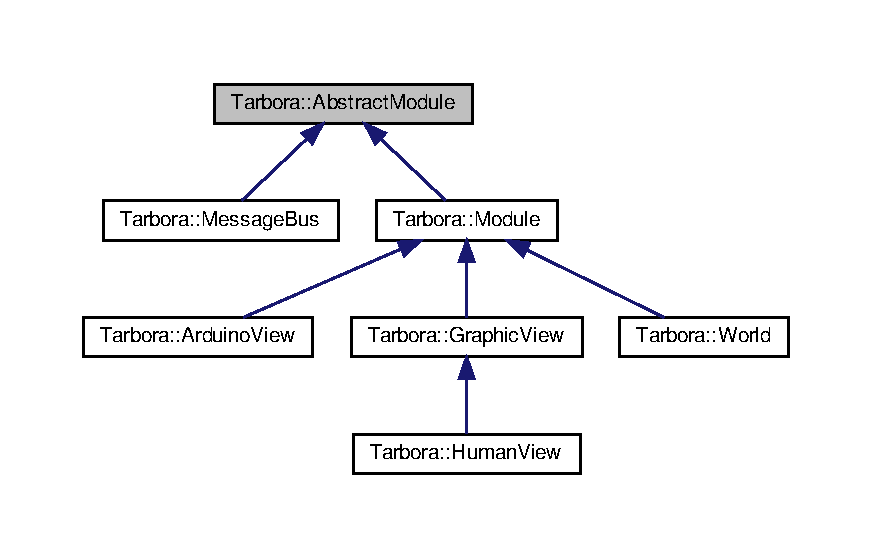
\includegraphics[width=350pt]{classTarbora_1_1AbstractModule__inherit__graph}
\end{center}
\end{figure}
\subsection*{Public Member Functions}
\begin{DoxyCompactItemize}
\item 
virtual void \hyperlink{classTarbora_1_1AbstractModule_acfb70b92b109b5e8ceae997c8629180a}{run} (const std\+::string \&name=\char`\"{}Unamed \hyperlink{classTarbora_1_1Module}{Module}\char`\"{})=0
\begin{DoxyCompactList}\small\item\em Start this module\textquotesingle{}s loop. \end{DoxyCompactList}\item 
void \hyperlink{classTarbora_1_1AbstractModule_ae65c482cc7cca2aae3e24811880c6313}{run\+Thread} (const std\+::string \&name=\char`\"{}Unamed \hyperlink{classTarbora_1_1Module}{Module}\char`\"{})
\begin{DoxyCompactList}\small\item\em Start this module\textquotesingle{}s loop in a new thread. \end{DoxyCompactList}\item 
\mbox{\Hypertarget{classTarbora_1_1AbstractModule_a3b1cc88ec4fc5c1351e5f4abe0e25948}\label{classTarbora_1_1AbstractModule_a3b1cc88ec4fc5c1351e5f4abe0e25948}} 
void \hyperlink{classTarbora_1_1AbstractModule_a3b1cc88ec4fc5c1351e5f4abe0e25948}{close} ()
\begin{DoxyCompactList}\small\item\em Stop this module\textquotesingle{}s loop. \end{DoxyCompactList}\end{DoxyCompactItemize}
\subsection*{Protected Attributes}
\begin{DoxyCompactItemize}
\item 
\mbox{\Hypertarget{classTarbora_1_1AbstractModule_aa13dfaed16573bef7cce22a473616bd5}\label{classTarbora_1_1AbstractModule_aa13dfaed16573bef7cce22a473616bd5}} 
bool {\bfseries using\+\_\+thread\+\_\+}
\end{DoxyCompactItemize}
\subsection*{Static Protected Attributes}
\begin{DoxyCompactItemize}
\item 
\mbox{\Hypertarget{classTarbora_1_1AbstractModule_a66ab779015a191a3188b1f91925e592b}\label{classTarbora_1_1AbstractModule_a66ab779015a191a3188b1f91925e592b}} 
static bool {\bfseries run\+\_\+} = true
\end{DoxyCompactItemize}


\subsection{Detailed Description}
Each of the parts that compose the Engine. 

\subsection{Member Function Documentation}
\mbox{\Hypertarget{classTarbora_1_1AbstractModule_acfb70b92b109b5e8ceae997c8629180a}\label{classTarbora_1_1AbstractModule_acfb70b92b109b5e8ceae997c8629180a}} 
\index{Tarbora\+::\+Abstract\+Module@{Tarbora\+::\+Abstract\+Module}!run@{run}}
\index{run@{run}!Tarbora\+::\+Abstract\+Module@{Tarbora\+::\+Abstract\+Module}}
\subsubsection{\texorpdfstring{run()}{run()}}
{\footnotesize\ttfamily virtual void Tarbora\+::\+Abstract\+Module\+::run (\begin{DoxyParamCaption}\item[{const std\+::string \&}]{name = {\ttfamily \char`\"{}Unamed~\hyperlink{classTarbora_1_1Module}{Module}\char`\"{}} }\end{DoxyParamCaption})\hspace{0.3cm}{\ttfamily [pure virtual]}}



Start this module\textquotesingle{}s loop. 

All modules should stop when Abstract\+Module\+::run\+\_\+ is set to false. 
\begin{DoxyParams}{Parameters}
{\em name} & The name of the module, only used for the profiler. \\
\hline
\end{DoxyParams}


Implemented in \hyperlink{classTarbora_1_1Module_a8c0352045b21b985d3798caa3190c70b}{Tarbora\+::\+Module}.

\mbox{\Hypertarget{classTarbora_1_1AbstractModule_ae65c482cc7cca2aae3e24811880c6313}\label{classTarbora_1_1AbstractModule_ae65c482cc7cca2aae3e24811880c6313}} 
\index{Tarbora\+::\+Abstract\+Module@{Tarbora\+::\+Abstract\+Module}!run\+Thread@{run\+Thread}}
\index{run\+Thread@{run\+Thread}!Tarbora\+::\+Abstract\+Module@{Tarbora\+::\+Abstract\+Module}}
\subsubsection{\texorpdfstring{run\+Thread()}{runThread()}}
{\footnotesize\ttfamily void Tarbora\+::\+Abstract\+Module\+::run\+Thread (\begin{DoxyParamCaption}\item[{const std\+::string \&}]{name = {\ttfamily \char`\"{}Unamed~\hyperlink{classTarbora_1_1Module}{Module}\char`\"{}} }\end{DoxyParamCaption})}



Start this module\textquotesingle{}s loop in a new thread. 


\begin{DoxyParams}{Parameters}
{\em name} & The name of the module, only used for the profiler. \\
\hline
\end{DoxyParams}


The documentation for this class was generated from the following files\+:\begin{DoxyCompactItemize}
\item 
Tarbora/\+Framework/\+Module/Abstract\+Module.\+hpp\item 
Tarbora/\+Framework/\+Module/Abstract\+Module.\+cpp\end{DoxyCompactItemize}

\hypertarget{classTarbora_1_1Message_1_1Actor}{}\section{Tarbora\+:\+:Message\+:\+:Actor Class Reference}
\label{classTarbora_1_1Message_1_1Actor}\index{Tarbora\+::\+Message\+::\+Actor@{Tarbora\+::\+Message\+::\+Actor}}


Inheritance diagram for Tarbora\+:\+:Message\+:\+:Actor\+:
\nopagebreak
\begin{figure}[H]
\begin{center}
\leavevmode
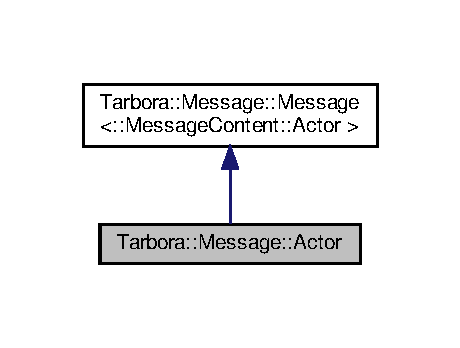
\includegraphics[width=221pt]{classTarbora_1_1Message_1_1Actor__inherit__graph}
\end{center}
\end{figure}


Collaboration diagram for Tarbora\+:\+:Message\+:\+:Actor\+:
\nopagebreak
\begin{figure}[H]
\begin{center}
\leavevmode
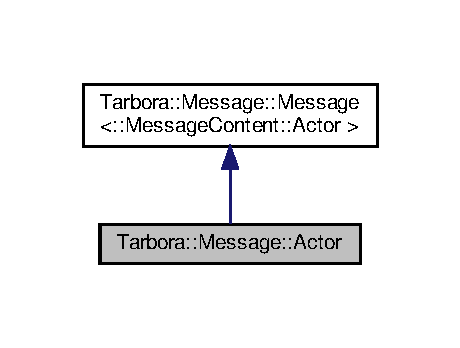
\includegraphics[width=221pt]{classTarbora_1_1Message_1_1Actor__coll__graph}
\end{center}
\end{figure}
\subsection*{Public Member Functions}
\begin{DoxyCompactItemize}
\item 
\mbox{\Hypertarget{classTarbora_1_1Message_1_1Actor_ad87e1dac0017c3c1f10dbcf93642e07b}\label{classTarbora_1_1Message_1_1Actor_ad87e1dac0017c3c1f10dbcf93642e07b}} 
{\bfseries Actor} (const \hyperlink{classTarbora_1_1MessageBody}{Message\+Body} \&m)
\item 
\mbox{\Hypertarget{classTarbora_1_1Message_1_1Actor_a27058490217da23f5398da551d3849a7}\label{classTarbora_1_1Message_1_1Actor_a27058490217da23f5398da551d3849a7}} 
{\bfseries Actor} (const Actor\+Id \&id)
\item 
\mbox{\Hypertarget{classTarbora_1_1Message_1_1Actor_a62c0d69a2bfca11efd8d34998d5e1ac5}\label{classTarbora_1_1Message_1_1Actor_a62c0d69a2bfca11efd8d34998d5e1ac5}} 
const Actor\+Id \& {\bfseries get\+Id} ()
\end{DoxyCompactItemize}
\subsection*{Additional Inherited Members}


The documentation for this class was generated from the following files\+:\begin{DoxyCompactItemize}
\item 
Tarbora/\+Messages/Basic\+Messages.\+hpp\item 
Tarbora/\+Messages/Basic\+Messages.\+cpp\end{DoxyCompactItemize}

\hypertarget{classTarbora_1_1ActorModel}{}\section{Tarbora\+:\+:Actor\+Model Class Reference}
\label{classTarbora_1_1ActorModel}\index{Tarbora\+::\+Actor\+Model@{Tarbora\+::\+Actor\+Model}}


Inheritance diagram for Tarbora\+:\+:Actor\+Model\+:
\nopagebreak
\begin{figure}[H]
\begin{center}
\leavevmode
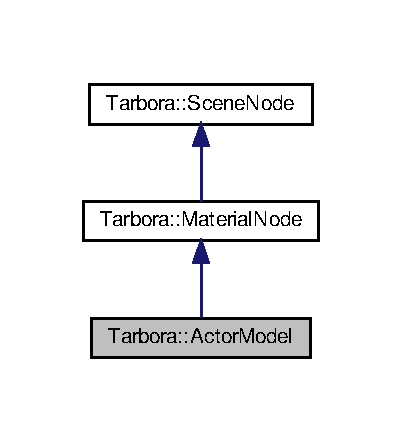
\includegraphics[width=193pt]{classTarbora_1_1ActorModel__inherit__graph}
\end{center}
\end{figure}


Collaboration diagram for Tarbora\+:\+:Actor\+Model\+:
\nopagebreak
\begin{figure}[H]
\begin{center}
\leavevmode
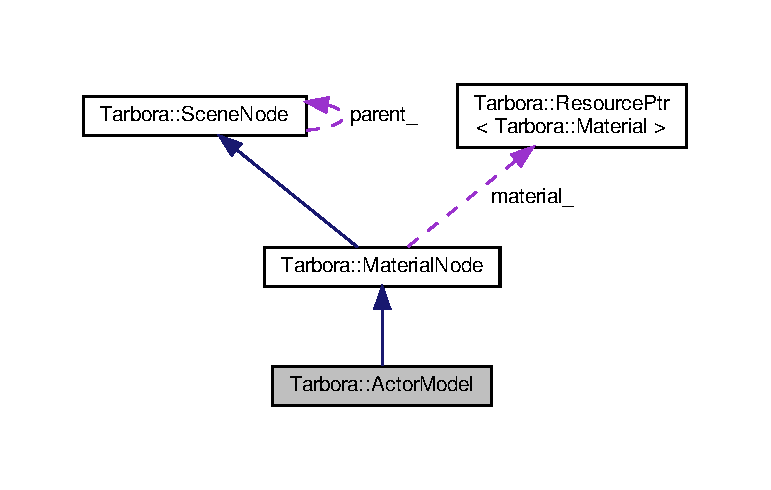
\includegraphics[width=350pt]{classTarbora_1_1ActorModel__coll__graph}
\end{center}
\end{figure}
\subsection*{Public Member Functions}
\begin{DoxyCompactItemize}
\item 
\mbox{\Hypertarget{classTarbora_1_1ActorModel_a1fefe619a840e2bbdf214e5d44962193}\label{classTarbora_1_1ActorModel_a1fefe619a840e2bbdf214e5d44962193}} 
{\bfseries Actor\+Model} (const Actor\+Id \&id, Render\+Pass render\+\_\+pass, const std\+::string \&model, const std\+::string \&material)
\item 
\mbox{\Hypertarget{classTarbora_1_1ActorModel_a444103ab29247d23375fe2a55392fae0}\label{classTarbora_1_1ActorModel_a444103ab29247d23375fe2a55392fae0}} 
std\+::shared\+\_\+ptr$<$ \hyperlink{classTarbora_1_1MeshNode}{Mesh\+Node} $>$ {\bfseries create\+Node} (const Actor\+Id \&id, Render\+Pass render\+\_\+pass, \hyperlink{classTarbora_1_1LuaTable}{Lua\+Table} table)
\item 
\mbox{\Hypertarget{classTarbora_1_1ActorModel_a162b40dc0f465add232c332fd7899610}\label{classTarbora_1_1ActorModel_a162b40dc0f465add232c332fd7899610}} 
std\+::shared\+\_\+ptr$<$ \hyperlink{classTarbora_1_1Camera}{Camera} $>$ {\bfseries create\+Camera} (const Actor\+Id \&id, \hyperlink{classTarbora_1_1LuaTable}{Lua\+Table} table)
\item 
\mbox{\Hypertarget{classTarbora_1_1ActorModel_a7c6a17305abb923b03a190e90b4f856e}\label{classTarbora_1_1ActorModel_a7c6a17305abb923b03a190e90b4f856e}} 
virtual void {\bfseries update} (\hyperlink{classTarbora_1_1Scene}{Scene} $\ast$scene, float delta\+\_\+time) override
\item 
\mbox{\Hypertarget{classTarbora_1_1ActorModel_a896fc0026eeed7a5527846711364cd88}\label{classTarbora_1_1ActorModel_a896fc0026eeed7a5527846711364cd88}} 
virtual std\+::shared\+\_\+ptr$<$ \hyperlink{classTarbora_1_1SceneNode}{Scene\+Node} $>$ {\bfseries get\+Child} (const std\+::string \&name) override
\item 
\mbox{\Hypertarget{classTarbora_1_1ActorModel_ae6ddda6bd0f911223020741eaa0e7694}\label{classTarbora_1_1ActorModel_ae6ddda6bd0f911223020741eaa0e7694}} 
void {\bfseries animate} (const std\+::string \&name, const std\+::string \&file=\char`\"{}\char`\"{})
\item 
\mbox{\Hypertarget{classTarbora_1_1ActorModel_a9c2a219815c5952de9aa1b4cd298b23d}\label{classTarbora_1_1ActorModel_a9c2a219815c5952de9aa1b4cd298b23d}} 
const std\+::string \& {\bfseries get\+Model} ()
\item 
\mbox{\Hypertarget{classTarbora_1_1ActorModel_a2955e28f4e1ab4fcb81affcbcd04cbd5}\label{classTarbora_1_1ActorModel_a2955e28f4e1ab4fcb81affcbcd04cbd5}} 
Render\+Pass {\bfseries get\+Render\+Pass} ()
\end{DoxyCompactItemize}
\subsection*{Friends}
\begin{DoxyCompactItemize}
\item 
\mbox{\Hypertarget{classTarbora_1_1ActorModel_a7899599edce4988a894c8e7431e7bb85}\label{classTarbora_1_1ActorModel_a7899599edce4988a894c8e7431e7bb85}} 
class {\bfseries Animation\+Controller}
\end{DoxyCompactItemize}
\subsection*{Additional Inherited Members}


The documentation for this class was generated from the following files\+:\begin{DoxyCompactItemize}
\item 
Tarbora/\+Views/\+Graphic\+Views/Actor\+Model.\+hpp\item 
Tarbora/\+Views/\+Graphic\+Views/Actor\+Model.\+cpp\end{DoxyCompactItemize}

\hypertarget{classTarbora_1_1ActorMotionState}{}\section{Tarbora\+:\+:Actor\+Motion\+State Class Reference}
\label{classTarbora_1_1ActorMotionState}\index{Tarbora\+::\+Actor\+Motion\+State@{Tarbora\+::\+Actor\+Motion\+State}}


Inheritance diagram for Tarbora\+:\+:Actor\+Motion\+State\+:\nopagebreak
\begin{figure}[H]
\begin{center}
\leavevmode
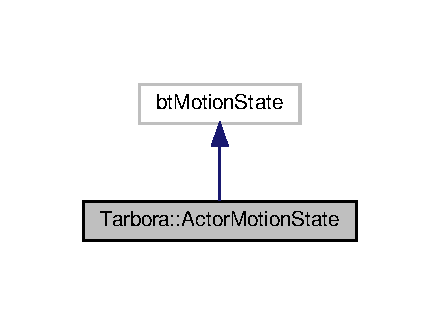
\includegraphics[width=211pt]{classTarbora_1_1ActorMotionState__inherit__graph}
\end{center}
\end{figure}


Collaboration diagram for Tarbora\+:\+:Actor\+Motion\+State\+:\nopagebreak
\begin{figure}[H]
\begin{center}
\leavevmode
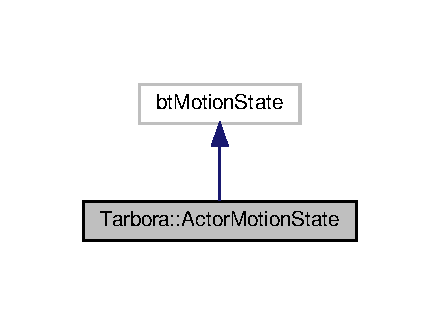
\includegraphics[width=211pt]{classTarbora_1_1ActorMotionState__coll__graph}
\end{center}
\end{figure}
\subsection*{Public Member Functions}
\begin{DoxyCompactItemize}
\item 
\mbox{\Hypertarget{classTarbora_1_1ActorMotionState_a9f0f8dfe3b52a74c0dff5196629f28c9}\label{classTarbora_1_1ActorMotionState_a9f0f8dfe3b52a74c0dff5196629f28c9}} 
{\bfseries Actor\+Motion\+State} (glm\+::mat4 const \&transform)
\item 
\mbox{\Hypertarget{classTarbora_1_1ActorMotionState_a6ca1b1961e95b7469e9dbef6d32f38e4}\label{classTarbora_1_1ActorMotionState_a6ca1b1961e95b7469e9dbef6d32f38e4}} 
virtual void {\bfseries get\+World\+Transform} (bt\+Transform \&transform) const
\item 
\mbox{\Hypertarget{classTarbora_1_1ActorMotionState_a116151bb38d94aede50f35841bb03e6b}\label{classTarbora_1_1ActorMotionState_a116151bb38d94aede50f35841bb03e6b}} 
virtual void {\bfseries set\+World\+Transform} (const bt\+Transform \&transform)
\item 
\mbox{\Hypertarget{classTarbora_1_1ActorMotionState_aebdbbe65dc6e5b8826cc500baf5f0318}\label{classTarbora_1_1ActorMotionState_aebdbbe65dc6e5b8826cc500baf5f0318}} 
void {\bfseries get\+World\+Transform} (glm\+::mat4 \&transform) const
\item 
\mbox{\Hypertarget{classTarbora_1_1ActorMotionState_ac39c57708b091d92a0812f9cda68e7bb}\label{classTarbora_1_1ActorMotionState_ac39c57708b091d92a0812f9cda68e7bb}} 
void {\bfseries set\+World\+Transform} (const glm\+::mat4 \&transform)
\item 
\mbox{\Hypertarget{classTarbora_1_1ActorMotionState_ab79ee121003e3adda3c77c210dadc058}\label{classTarbora_1_1ActorMotionState_ab79ee121003e3adda3c77c210dadc058}} 
glm\+::vec3 {\bfseries get\+Position} ()
\item 
\mbox{\Hypertarget{classTarbora_1_1ActorMotionState_af57e028d47be8d142a01c61c25952eb0}\label{classTarbora_1_1ActorMotionState_af57e028d47be8d142a01c61c25952eb0}} 
glm\+::mat3 {\bfseries get\+Rotation} ()
\end{DoxyCompactItemize}
\subsection*{Public Attributes}
\begin{DoxyCompactItemize}
\item 
\mbox{\Hypertarget{classTarbora_1_1ActorMotionState_a89476c358757187de24d4917f4986b93}\label{classTarbora_1_1ActorMotionState_a89476c358757187de24d4917f4986b93}} 
glm\+::mat4 {\bfseries m\+\_\+\+Transform}
\end{DoxyCompactItemize}


The documentation for this class was generated from the following files\+:\begin{DoxyCompactItemize}
\item 
Tarbora/\+Framework/\+Physics\+Engine/inc/Physics\+Engine.\+hpp\item 
Tarbora/\+Framework/\+Physics\+Engine/src/Physics\+Engine.\+cpp\end{DoxyCompactItemize}

\hypertarget{classTarbora_1_1AnimatedNode}{}\section{Tarbora\+:\+:Animated\+Node Class Reference}
\label{classTarbora_1_1AnimatedNode}\index{Tarbora\+::\+Animated\+Node@{Tarbora\+::\+Animated\+Node}}


Inheritance diagram for Tarbora\+:\+:Animated\+Node\+:
\nopagebreak
\begin{figure}[H]
\begin{center}
\leavevmode
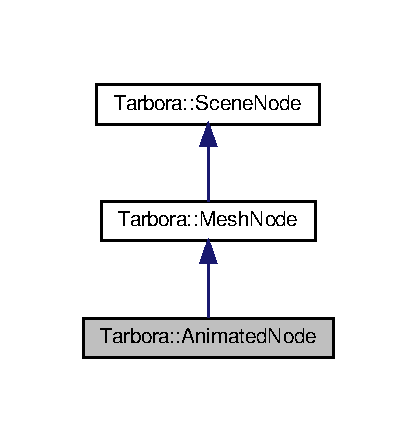
\includegraphics[width=200pt]{classTarbora_1_1AnimatedNode__inherit__graph}
\end{center}
\end{figure}


Collaboration diagram for Tarbora\+:\+:Animated\+Node\+:
\nopagebreak
\begin{figure}[H]
\begin{center}
\leavevmode
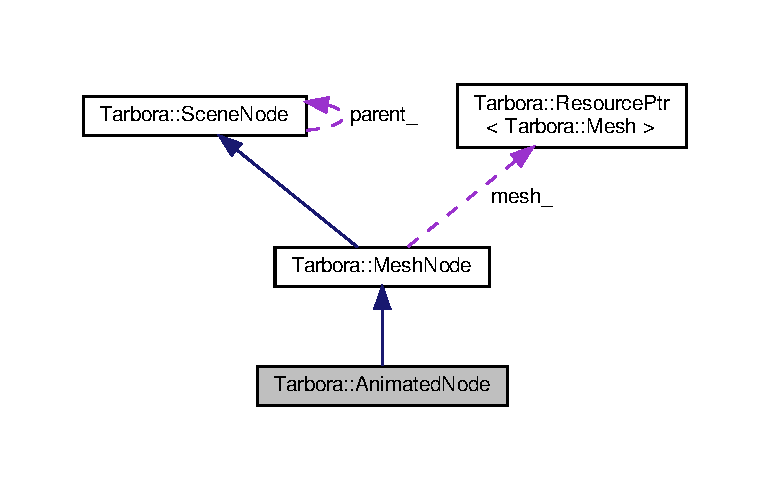
\includegraphics[width=350pt]{classTarbora_1_1AnimatedNode__coll__graph}
\end{center}
\end{figure}
\subsection*{Public Member Functions}
\begin{DoxyCompactItemize}
\item 
\mbox{\Hypertarget{classTarbora_1_1AnimatedNode_a9a53e7180e339f37d11c2a565efa36f1}\label{classTarbora_1_1AnimatedNode_a9a53e7180e339f37d11c2a565efa36f1}} 
{\bfseries Animated\+Node} (const Actor\+Id \&id, const std\+::string \&name, Render\+Pass render\+\_\+pass, const std\+::string \&mesh)
\item 
\mbox{\Hypertarget{classTarbora_1_1AnimatedNode_af6e8caa16b073c2c4e9a74ba9c4385d5}\label{classTarbora_1_1AnimatedNode_af6e8caa16b073c2c4e9a74ba9c4385d5}} 
virtual const std\+::string {\bfseries get\+Node\+Type} ()
\item 
\mbox{\Hypertarget{classTarbora_1_1AnimatedNode_ab2ca2c3bc1ef81c51cc6060f5495ba2a}\label{classTarbora_1_1AnimatedNode_ab2ca2c3bc1ef81c51cc6060f5495ba2a}} 
virtual void {\bfseries draw} (\hyperlink{classTarbora_1_1Scene}{Scene} $\ast$scene, const glm\+::mat4 \&transform)
\item 
\mbox{\Hypertarget{classTarbora_1_1AnimatedNode_a6da3fadd5907f3970b6257ace4755bd4}\label{classTarbora_1_1AnimatedNode_a6da3fadd5907f3970b6257ace4755bd4}} 
void {\bfseries reset\+All} ()
\item 
\mbox{\Hypertarget{classTarbora_1_1AnimatedNode_af273bb9d74d9e41e2d602cd954e36562}\label{classTarbora_1_1AnimatedNode_af273bb9d74d9e41e2d602cd954e36562}} 
void {\bfseries set\+Position\+Animation} (const glm\+::vec3 \&position)
\item 
\mbox{\Hypertarget{classTarbora_1_1AnimatedNode_a6f1e6162f6a50ce39ce65b08cbc8a159}\label{classTarbora_1_1AnimatedNode_a6f1e6162f6a50ce39ce65b08cbc8a159}} 
void {\bfseries set\+Rotation\+Animation} (const glm\+::vec3 \&rotation)
\item 
\mbox{\Hypertarget{classTarbora_1_1AnimatedNode_a09bccc0e9e1e2450eeca7acbb58cc6ad}\label{classTarbora_1_1AnimatedNode_a09bccc0e9e1e2450eeca7acbb58cc6ad}} 
void {\bfseries set\+Rotation\+Animation} (const glm\+::quat \&rotation)
\item 
\mbox{\Hypertarget{classTarbora_1_1AnimatedNode_a2e5a5186a22248d950223b7224b6167c}\label{classTarbora_1_1AnimatedNode_a2e5a5186a22248d950223b7224b6167c}} 
void {\bfseries set\+Scale\+Animation} (const glm\+::vec3 \&scale)
\item 
\mbox{\Hypertarget{classTarbora_1_1AnimatedNode_ab2bc2200bbdacc8bb27573b8da0cdd00}\label{classTarbora_1_1AnimatedNode_ab2bc2200bbdacc8bb27573b8da0cdd00}} 
void {\bfseries set\+Global\+Scale\+Animation} (float scale)
\item 
\mbox{\Hypertarget{classTarbora_1_1AnimatedNode_a6b32e3442bbbd370d73cc61ac6e80514}\label{classTarbora_1_1AnimatedNode_a6b32e3442bbbd370d73cc61ac6e80514}} 
void {\bfseries set\+Uv\+Map\+Animation} (const glm\+::tvec2$<$ unsigned short $>$ \&uv)
\item 
\mbox{\Hypertarget{classTarbora_1_1AnimatedNode_a25054223d38704d2671a9f5214f94702}\label{classTarbora_1_1AnimatedNode_a25054223d38704d2671a9f5214f94702}} 
void {\bfseries set\+Color\+Primary\+Animation} (const glm\+::tvec3$<$ unsigned char $>$ \&color)
\item 
\mbox{\Hypertarget{classTarbora_1_1AnimatedNode_abc723035daccf254fa2e4e590ab8625c}\label{classTarbora_1_1AnimatedNode_abc723035daccf254fa2e4e590ab8625c}} 
void {\bfseries set\+Color\+Secondary\+Animation} (const glm\+::tvec3$<$ unsigned char $>$ \&color)
\item 
\mbox{\Hypertarget{classTarbora_1_1AnimatedNode_a606f8d404bd97a8524e3bd52434b9686}\label{classTarbora_1_1AnimatedNode_a606f8d404bd97a8524e3bd52434b9686}} 
void {\bfseries set\+Color\+Detail\+Animation} (const glm\+::tvec3$<$ unsigned char $>$ \&color)
\item 
\mbox{\Hypertarget{classTarbora_1_1AnimatedNode_a7a36adb6aecddf443a8d91f64b42d16a}\label{classTarbora_1_1AnimatedNode_a7a36adb6aecddf443a8d91f64b42d16a}} 
void {\bfseries set\+Color\+Detail2\+Animation} (const glm\+::tvec3$<$ unsigned char $>$ \&color)
\item 
\mbox{\Hypertarget{classTarbora_1_1AnimatedNode_a3992e83c9d856be4312c2a82818202f7}\label{classTarbora_1_1AnimatedNode_a3992e83c9d856be4312c2a82818202f7}} 
const glm\+::vec3 \& {\bfseries get\+Position\+Animation} ()
\item 
\mbox{\Hypertarget{classTarbora_1_1AnimatedNode_a60ed996f8227702ccc8afaf470629f54}\label{classTarbora_1_1AnimatedNode_a60ed996f8227702ccc8afaf470629f54}} 
const glm\+::quat \& {\bfseries get\+Rotation\+Animation} ()
\item 
\mbox{\Hypertarget{classTarbora_1_1AnimatedNode_a381ebd9c6caadd103e839b3faf6489ba}\label{classTarbora_1_1AnimatedNode_a381ebd9c6caadd103e839b3faf6489ba}} 
const glm\+::vec3 \& {\bfseries get\+Scale\+Animation} ()
\item 
\mbox{\Hypertarget{classTarbora_1_1AnimatedNode_a0fddc54e94bf50c435305043dc328ddc}\label{classTarbora_1_1AnimatedNode_a0fddc54e94bf50c435305043dc328ddc}} 
float {\bfseries get\+Global\+Scale\+Animation} ()
\item 
\mbox{\Hypertarget{classTarbora_1_1AnimatedNode_a184531fec66eb3f9e53c3432942b51d2}\label{classTarbora_1_1AnimatedNode_a184531fec66eb3f9e53c3432942b51d2}} 
const glm\+::tvec2$<$ unsigned short $>$ \& {\bfseries get\+Uv\+Map\+Animation} ()
\item 
\mbox{\Hypertarget{classTarbora_1_1AnimatedNode_a06713d98a7b6cb58aab0b88bca3516fb}\label{classTarbora_1_1AnimatedNode_a06713d98a7b6cb58aab0b88bca3516fb}} 
const glm\+::tvec3$<$ unsigned char $>$ \& {\bfseries get\+Color\+Primary\+Animation} ()
\item 
\mbox{\Hypertarget{classTarbora_1_1AnimatedNode_a5a24c0231010fc0ccc022eb6aed40a70}\label{classTarbora_1_1AnimatedNode_a5a24c0231010fc0ccc022eb6aed40a70}} 
const glm\+::tvec3$<$ unsigned char $>$ \& {\bfseries get\+Color\+Secondary\+Animation} ()
\item 
\mbox{\Hypertarget{classTarbora_1_1AnimatedNode_a2d401e3ab855f9190b1e75c491b7144e}\label{classTarbora_1_1AnimatedNode_a2d401e3ab855f9190b1e75c491b7144e}} 
const glm\+::tvec3$<$ unsigned char $>$ \& {\bfseries get\+Color\+Detail\+Animation} ()
\item 
\mbox{\Hypertarget{classTarbora_1_1AnimatedNode_abbf3c7d7ec39ab9ce0d2ba26c83d4f97}\label{classTarbora_1_1AnimatedNode_abbf3c7d7ec39ab9ce0d2ba26c83d4f97}} 
const glm\+::tvec3$<$ unsigned char $>$ \& {\bfseries get\+Color\+Detail2\+Animation} ()
\item 
\mbox{\Hypertarget{classTarbora_1_1AnimatedNode_a384a1b6cf9e5895aab591230cf95eb1b}\label{classTarbora_1_1AnimatedNode_a384a1b6cf9e5895aab591230cf95eb1b}} 
virtual glm\+::mat4 {\bfseries get\+Local\+Transform} ()
\item 
\mbox{\Hypertarget{classTarbora_1_1AnimatedNode_ab4b9aff67108cbdcae4384dec91e370b}\label{classTarbora_1_1AnimatedNode_ab4b9aff67108cbdcae4384dec91e370b}} 
virtual glm\+::mat4 {\bfseries get\+Deform} ()
\end{DoxyCompactItemize}
\subsection*{Protected Attributes}
\begin{DoxyCompactItemize}
\item 
\mbox{\Hypertarget{classTarbora_1_1AnimatedNode_a02fc79ea76ea1a7b2a5c34c92e215716}\label{classTarbora_1_1AnimatedNode_a02fc79ea76ea1a7b2a5c34c92e215716}} 
glm\+::vec3 {\bfseries position\+\_\+anim\+\_\+}
\item 
\mbox{\Hypertarget{classTarbora_1_1AnimatedNode_ace8df245f00cf87a48a9f25508415589}\label{classTarbora_1_1AnimatedNode_ace8df245f00cf87a48a9f25508415589}} 
glm\+::quat {\bfseries rotation\+\_\+anim\+\_\+}
\item 
\mbox{\Hypertarget{classTarbora_1_1AnimatedNode_a951070a55a9c75da3af2d6ae10f8c3ed}\label{classTarbora_1_1AnimatedNode_a951070a55a9c75da3af2d6ae10f8c3ed}} 
glm\+::vec3 {\bfseries scale\+\_\+anim\+\_\+}
\item 
\mbox{\Hypertarget{classTarbora_1_1AnimatedNode_a7941318652eed31b40cc44c5927c65e8}\label{classTarbora_1_1AnimatedNode_a7941318652eed31b40cc44c5927c65e8}} 
float {\bfseries global\+\_\+scale\+\_\+anim\+\_\+}
\item 
\mbox{\Hypertarget{classTarbora_1_1AnimatedNode_a03c3d13efeb19eee3cb774fafc77f62e}\label{classTarbora_1_1AnimatedNode_a03c3d13efeb19eee3cb774fafc77f62e}} 
glm\+::tvec2$<$ unsigned short $>$ {\bfseries uv\+\_\+map\+\_\+anim\+\_\+}
\item 
\mbox{\Hypertarget{classTarbora_1_1AnimatedNode_a5afaff7507ededc5f6cfb4ffef6b7d41}\label{classTarbora_1_1AnimatedNode_a5afaff7507ededc5f6cfb4ffef6b7d41}} 
glm\+::tvec3$<$ unsigned char $>$ {\bfseries color\+\_\+primary\+\_\+anim\+\_\+}
\item 
\mbox{\Hypertarget{classTarbora_1_1AnimatedNode_a594393a8878b86938f3552c1515cf7f7}\label{classTarbora_1_1AnimatedNode_a594393a8878b86938f3552c1515cf7f7}} 
glm\+::tvec3$<$ unsigned char $>$ {\bfseries color\+\_\+secondary\+\_\+anim\+\_\+}
\item 
\mbox{\Hypertarget{classTarbora_1_1AnimatedNode_a93916433f3bc22b7817a51b9a9ff5161}\label{classTarbora_1_1AnimatedNode_a93916433f3bc22b7817a51b9a9ff5161}} 
glm\+::tvec3$<$ unsigned char $>$ {\bfseries color\+\_\+detail\+\_\+anim\+\_\+}
\item 
\mbox{\Hypertarget{classTarbora_1_1AnimatedNode_a3b2b12634b95c0d9008dda3a1a96e666}\label{classTarbora_1_1AnimatedNode_a3b2b12634b95c0d9008dda3a1a96e666}} 
glm\+::tvec3$<$ unsigned char $>$ {\bfseries color\+\_\+detail2\+\_\+anim\+\_\+}
\end{DoxyCompactItemize}


The documentation for this class was generated from the following files\+:\begin{DoxyCompactItemize}
\item 
Tarbora/\+Views/\+Graphic\+Views/Scene\+Node.\+hpp\item 
Tarbora/\+Views/\+Graphic\+Views/Scene\+Node.\+cpp\end{DoxyCompactItemize}

\hypertarget{structTarbora_1_1Animation}{}\section{Tarbora\+:\+:Animation Struct Reference}
\label{structTarbora_1_1Animation}\index{Tarbora\+::\+Animation@{Tarbora\+::\+Animation}}
\subsection*{Public Member Functions}
\begin{DoxyCompactItemize}
\item 
\mbox{\Hypertarget{structTarbora_1_1Animation_ad126137d30e797c264694cfe200392c4}\label{structTarbora_1_1Animation_ad126137d30e797c264694cfe200392c4}} 
bool {\bfseries update} (float delta\+\_\+time, \hyperlink{classTarbora_1_1ActorModel}{Actor\+Model} $\ast$actor)
\item 
\mbox{\Hypertarget{structTarbora_1_1Animation_a21d9ea91e21a8ebe153aeb3ac5f1b034}\label{structTarbora_1_1Animation_a21d9ea91e21a8ebe153aeb3ac5f1b034}} 
{\footnotesize template$<$class T $>$ }\\T {\bfseries blend\+Property} (T value, T old\+\_\+value, const \hyperlink{structTarbora_1_1Animation}{Animation} $\ast$animation)
\item 
\mbox{\Hypertarget{structTarbora_1_1Animation_ad822c0f4505383d6c3f70f4a24d8b364}\label{structTarbora_1_1Animation_ad822c0f4505383d6c3f70f4a24d8b364}} 
{\footnotesize template$<$$>$ }\\glm\+::quat {\bfseries blend\+Property} (glm\+::quat value, glm\+::quat old\+\_\+value, const \hyperlink{structTarbora_1_1Animation}{Animation} $\ast$animation)
\end{DoxyCompactItemize}
\subsection*{Public Attributes}
\begin{DoxyCompactItemize}
\item 
\mbox{\Hypertarget{structTarbora_1_1Animation_a6a0ed549c9377e507e01019e45b2d904}\label{structTarbora_1_1Animation_a6a0ed549c9377e507e01019e45b2d904}} 
std\+::string {\bfseries name}
\item 
\mbox{\Hypertarget{structTarbora_1_1Animation_a459770a5d20a315344cde15dd0031ecb}\label{structTarbora_1_1Animation_a459770a5d20a315344cde15dd0031ecb}} 
std\+::string {\bfseries file}
\item 
\mbox{\Hypertarget{structTarbora_1_1Animation_a484d6813d70493bf607264eea0408cab}\label{structTarbora_1_1Animation_a484d6813d70493bf607264eea0408cab}} 
Blend\+Mode {\bfseries blend\+\_\+mode}
\item 
\mbox{\Hypertarget{structTarbora_1_1Animation_aeb4c3f740140709df580bc657eb425d5}\label{structTarbora_1_1Animation_aeb4c3f740140709df580bc657eb425d5}} 
float {\bfseries blend\+\_\+factor}
\item 
\mbox{\Hypertarget{structTarbora_1_1Animation_a0d88700240a0dfdf762d8b507d10c56a}\label{structTarbora_1_1Animation_a0d88700240a0dfdf762d8b507d10c56a}} 
float {\bfseries fade\+\_\+in\+\_\+timer}
\item 
\mbox{\Hypertarget{structTarbora_1_1Animation_a85519d8253039980c275ba4c12b1b1cf}\label{structTarbora_1_1Animation_a85519d8253039980c275ba4c12b1b1cf}} 
bool {\bfseries loop}
\item 
\mbox{\Hypertarget{structTarbora_1_1Animation_a6411f6a3a4b59760785e3d138b99fdc0}\label{structTarbora_1_1Animation_a6411f6a3a4b59760785e3d138b99fdc0}} 
float {\bfseries timer} \{0.f\}
\item 
\mbox{\Hypertarget{structTarbora_1_1Animation_a215ea2011d37bfe6d43b78a9dc00a01a}\label{structTarbora_1_1Animation_a215ea2011d37bfe6d43b78a9dc00a01a}} 
float {\bfseries duration} \{0.f\}
\item 
\mbox{\Hypertarget{structTarbora_1_1Animation_a1d255cfd1429471dcf5d322ca34860c6}\label{structTarbora_1_1Animation_a1d255cfd1429471dcf5d322ca34860c6}} 
float {\bfseries fade\+\_\+out\+\_\+timer} \{-\/1.f\}
\end{DoxyCompactItemize}


The documentation for this struct was generated from the following files\+:\begin{DoxyCompactItemize}
\item 
Tarbora/\+Views/\+Graphic\+Views/Animation\+Controller.\+hpp\item 
Tarbora/\+Views/\+Graphic\+Views/Animation\+Controller.\+cpp\end{DoxyCompactItemize}

\hypertarget{classTarbora_1_1AnimationComponent}{}\section{Tarbora\+:\+:Animation\+Component Class Reference}
\label{classTarbora_1_1AnimationComponent}\index{Tarbora\+::\+Animation\+Component@{Tarbora\+::\+Animation\+Component}}


Inheritance diagram for Tarbora\+:\+:Animation\+Component\+:
\nopagebreak
\begin{figure}[H]
\begin{center}
\leavevmode
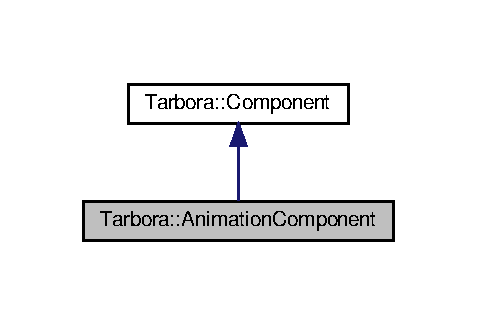
\includegraphics[width=229pt]{classTarbora_1_1AnimationComponent__inherit__graph}
\end{center}
\end{figure}


Collaboration diagram for Tarbora\+:\+:Animation\+Component\+:
\nopagebreak
\begin{figure}[H]
\begin{center}
\leavevmode
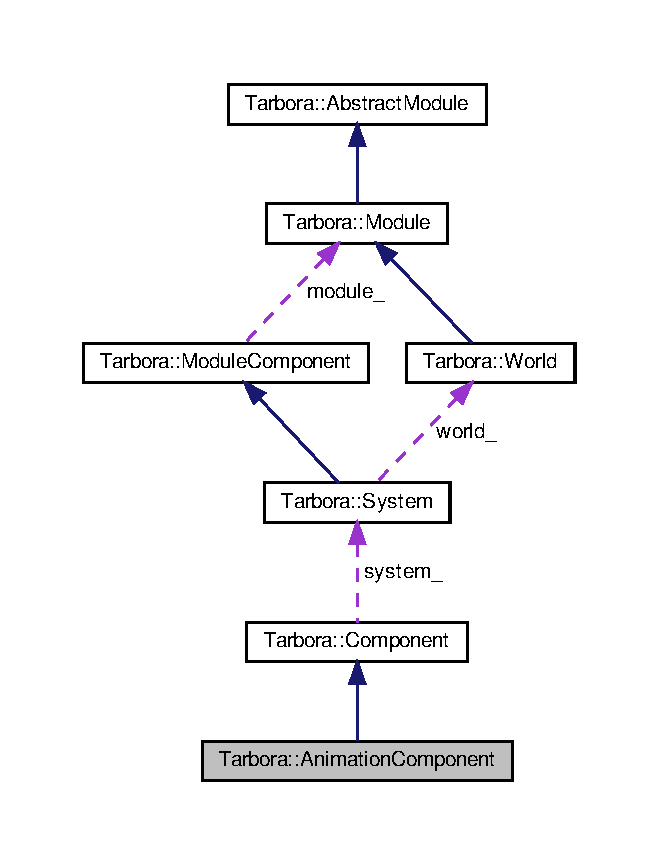
\includegraphics[width=316pt]{classTarbora_1_1AnimationComponent__coll__graph}
\end{center}
\end{figure}
\subsection*{Public Member Functions}
\begin{DoxyCompactItemize}
\item 
\mbox{\Hypertarget{classTarbora_1_1AnimationComponent_a80c77d7fedaca33e0ae0898da08bcf2b}\label{classTarbora_1_1AnimationComponent_a80c77d7fedaca33e0ae0898da08bcf2b}} 
{\bfseries Animation\+Component} (\hyperlink{classTarbora_1_1System}{System} $\ast$s, const Actor\+Id \&id, const \hyperlink{classTarbora_1_1LuaTable}{Lua\+Table} \&table)
\item 
\mbox{\Hypertarget{classTarbora_1_1AnimationComponent_a82fbbb5ad1b752c8cba225796812351e}\label{classTarbora_1_1AnimationComponent_a82fbbb5ad1b752c8cba225796812351e}} 
void {\bfseries set} (const std\+::string \&animation)
\item 
\mbox{\Hypertarget{classTarbora_1_1AnimationComponent_affc9c4991f3387ad6996e17b0bdc6970}\label{classTarbora_1_1AnimationComponent_affc9c4991f3387ad6996e17b0bdc6970}} 
const std\+::string \& {\bfseries get} ()
\end{DoxyCompactItemize}
\subsection*{Additional Inherited Members}


The documentation for this class was generated from the following files\+:\begin{DoxyCompactItemize}
\item 
Tarbora/\+Logic/Animation\+Component.\+hpp\item 
Tarbora/\+Logic/Animation\+Component.\+cpp\end{DoxyCompactItemize}

\hypertarget{classTarbora_1_1AnimationController}{}\section{Tarbora\+:\+:Animation\+Controller Class Reference}
\label{classTarbora_1_1AnimationController}\index{Tarbora\+::\+Animation\+Controller@{Tarbora\+::\+Animation\+Controller}}
\subsection*{Public Member Functions}
\begin{DoxyCompactItemize}
\item 
\mbox{\Hypertarget{classTarbora_1_1AnimationController_a3646c4571530d81d0b0dc58e0aab08fe}\label{classTarbora_1_1AnimationController_a3646c4571530d81d0b0dc58e0aab08fe}} 
{\bfseries Animation\+Controller} (\hyperlink{classTarbora_1_1ActorModel}{Actor\+Model} $\ast$actor, std\+::string animations\+\_\+file)
\item 
\mbox{\Hypertarget{classTarbora_1_1AnimationController_a5e16fba3e32db6e6ac061a54ae9949b1}\label{classTarbora_1_1AnimationController_a5e16fba3e32db6e6ac061a54ae9949b1}} 
void {\bfseries Update} (float delta\+Time)
\item 
\mbox{\Hypertarget{classTarbora_1_1AnimationController_a82ebfc6b041c20700252196c7aefc656}\label{classTarbora_1_1AnimationController_a82ebfc6b041c20700252196c7aefc656}} 
void {\bfseries Set\+Animation} (std\+::string animation\+\_\+name)
\item 
\mbox{\Hypertarget{classTarbora_1_1AnimationController_aa5f632bc3c8cea954f083f52d715ccf1}\label{classTarbora_1_1AnimationController_aa5f632bc3c8cea954f083f52d715ccf1}} 
void {\bfseries Update\+Animation} (float frame)
\end{DoxyCompactItemize}


The documentation for this class was generated from the following files\+:\begin{DoxyCompactItemize}
\item 
Tarbora/\+Views/\+Graphic\+Views/inc/Animation\+Controller.\+hpp\item 
Tarbora/\+Views/\+Graphic\+Views/src/Animation\+Controller.\+cpp\end{DoxyCompactItemize}

\hypertarget{classTarbora_1_1AnimationSystem}{}\section{Tarbora\+:\+:Animation\+System Class Reference}
\label{classTarbora_1_1AnimationSystem}\index{Tarbora\+::\+Animation\+System@{Tarbora\+::\+Animation\+System}}


Inheritance diagram for Tarbora\+:\+:Animation\+System\+:\nopagebreak
\begin{figure}[H]
\begin{center}
\leavevmode
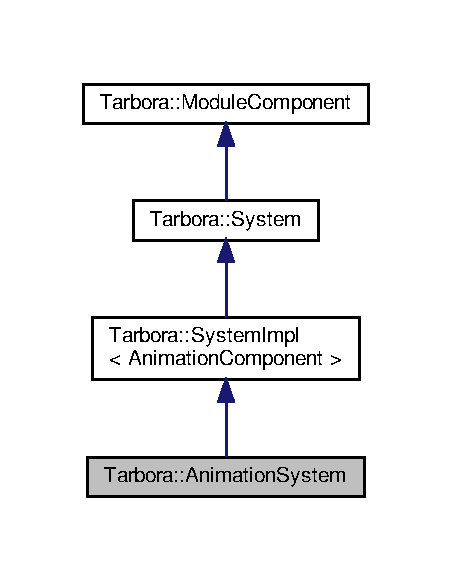
\includegraphics[width=217pt]{classTarbora_1_1AnimationSystem__inherit__graph}
\end{center}
\end{figure}


Collaboration diagram for Tarbora\+:\+:Animation\+System\+:\nopagebreak
\begin{figure}[H]
\begin{center}
\leavevmode
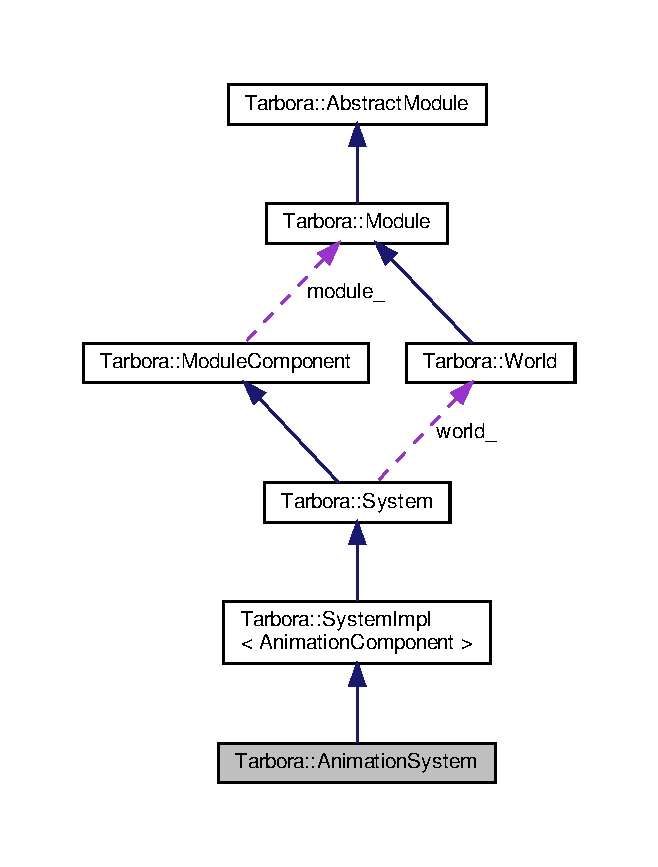
\includegraphics[width=316pt]{classTarbora_1_1AnimationSystem__coll__graph}
\end{center}
\end{figure}
\subsection*{Public Member Functions}
\begin{DoxyCompactItemize}
\item 
\mbox{\Hypertarget{classTarbora_1_1AnimationSystem_a15c1e060a4dffe2fae17adb2b1984500}\label{classTarbora_1_1AnimationSystem_a15c1e060a4dffe2fae17adb2b1984500}} 
{\bfseries Animation\+System} (\hyperlink{classTarbora_1_1World}{World} $\ast$w)
\item 
\mbox{\Hypertarget{classTarbora_1_1AnimationSystem_a883d0cc7a780db4b7713b6c64fb50e13}\label{classTarbora_1_1AnimationSystem_a883d0cc7a780db4b7713b6c64fb50e13}} 
virtual void {\bfseries init} (const Actor\+Id \&id)
\end{DoxyCompactItemize}
\subsection*{Static Public Member Functions}
\begin{DoxyCompactItemize}
\item 
\mbox{\Hypertarget{classTarbora_1_1AnimationSystem_af789b917c68f8b9d5b74ede0eeaae381}\label{classTarbora_1_1AnimationSystem_af789b917c68f8b9d5b74ede0eeaae381}} 
static std\+::string {\bfseries get\+Name} ()
\end{DoxyCompactItemize}
\subsection*{Additional Inherited Members}


The documentation for this class was generated from the following files\+:\begin{DoxyCompactItemize}
\item 
Tarbora/\+Logic/Animation\+Component.\+hpp\item 
Tarbora/\+Logic/Animation\+Component.\+cpp\end{DoxyCompactItemize}

\hypertarget{classTarbora_1_1Message_1_1ApplyPhysics}{}\section{Tarbora\+:\+:Message\+:\+:Apply\+Physics Class Reference}
\label{classTarbora_1_1Message_1_1ApplyPhysics}\index{Tarbora\+::\+Message\+::\+Apply\+Physics@{Tarbora\+::\+Message\+::\+Apply\+Physics}}


Inheritance diagram for Tarbora\+:\+:Message\+:\+:Apply\+Physics\+:
\nopagebreak
\begin{figure}[H]
\begin{center}
\leavevmode
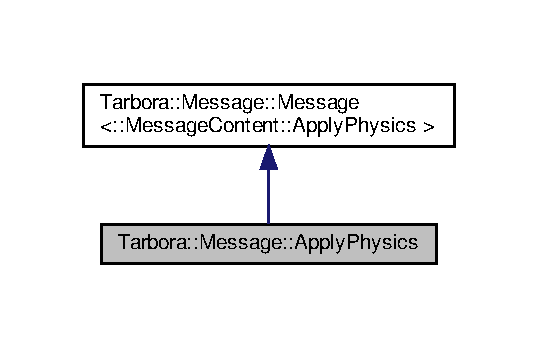
\includegraphics[width=258pt]{classTarbora_1_1Message_1_1ApplyPhysics__inherit__graph}
\end{center}
\end{figure}


Collaboration diagram for Tarbora\+:\+:Message\+:\+:Apply\+Physics\+:
\nopagebreak
\begin{figure}[H]
\begin{center}
\leavevmode
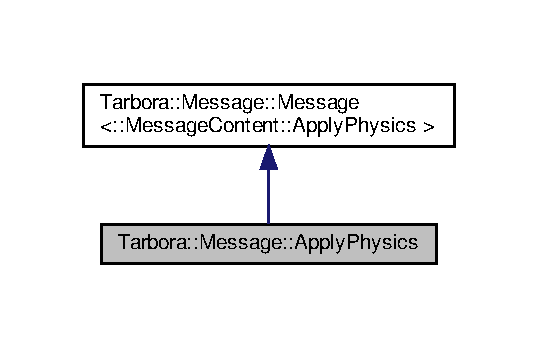
\includegraphics[width=258pt]{classTarbora_1_1Message_1_1ApplyPhysics__coll__graph}
\end{center}
\end{figure}
\subsection*{Public Member Functions}
\begin{DoxyCompactItemize}
\item 
\mbox{\Hypertarget{classTarbora_1_1Message_1_1ApplyPhysics_aaf094749948c404ccbcb22280f25c982}\label{classTarbora_1_1Message_1_1ApplyPhysics_aaf094749948c404ccbcb22280f25c982}} 
{\bfseries Apply\+Physics} (const \hyperlink{classTarbora_1_1MessageBody}{Message\+Body} \&m)
\item 
\mbox{\Hypertarget{classTarbora_1_1Message_1_1ApplyPhysics_a39dfe4cee807aaec0ff7bcac04536adf}\label{classTarbora_1_1Message_1_1ApplyPhysics_a39dfe4cee807aaec0ff7bcac04536adf}} 
{\bfseries Apply\+Physics} (const Actor\+Id \&id, const glm\+::vec3 \&direction)
\item 
\mbox{\Hypertarget{classTarbora_1_1Message_1_1ApplyPhysics_a716a5a031efecf77d7f47db3edf2955d}\label{classTarbora_1_1Message_1_1ApplyPhysics_a716a5a031efecf77d7f47db3edf2955d}} 
const Actor\+Id \& {\bfseries get\+Id} ()
\item 
\mbox{\Hypertarget{classTarbora_1_1Message_1_1ApplyPhysics_a80492a21ec96154ef77229d040de6d0d}\label{classTarbora_1_1Message_1_1ApplyPhysics_a80492a21ec96154ef77229d040de6d0d}} 
glm\+::vec3 {\bfseries get\+Direction} ()
\item 
\mbox{\Hypertarget{classTarbora_1_1Message_1_1ApplyPhysics_a2f7b0de1155f888ae3ad29e28187280e}\label{classTarbora_1_1Message_1_1ApplyPhysics_a2f7b0de1155f888ae3ad29e28187280e}} 
bool {\bfseries has\+Direction} ()
\end{DoxyCompactItemize}
\subsection*{Additional Inherited Members}


The documentation for this class was generated from the following file\+:\begin{DoxyCompactItemize}
\item 
Tarbora/\+Messages/Basic\+Messages.\+hpp\end{DoxyCompactItemize}

\hypertarget{classTarbora_1_1ArduinoView}{}\section{Tarbora\+:\+:Arduino\+View Class Reference}
\label{classTarbora_1_1ArduinoView}\index{Tarbora\+::\+Arduino\+View@{Tarbora\+::\+Arduino\+View}}


Inheritance diagram for Tarbora\+:\+:Arduino\+View\+:\nopagebreak
\begin{figure}[H]
\begin{center}
\leavevmode
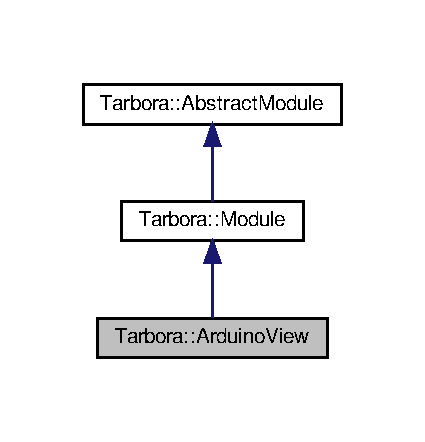
\includegraphics[width=204pt]{classTarbora_1_1ArduinoView__inherit__graph}
\end{center}
\end{figure}


Collaboration diagram for Tarbora\+:\+:Arduino\+View\+:\nopagebreak
\begin{figure}[H]
\begin{center}
\leavevmode
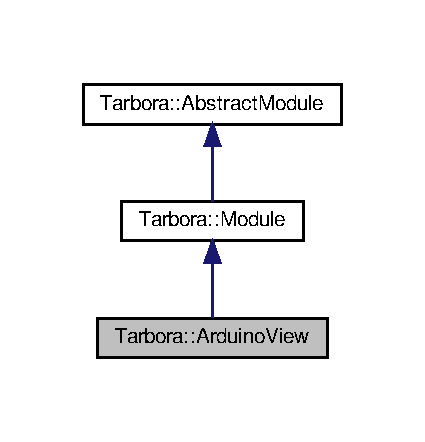
\includegraphics[width=204pt]{classTarbora_1_1ArduinoView__coll__graph}
\end{center}
\end{figure}
\subsection*{Public Member Functions}
\begin{DoxyCompactItemize}
\item 
\mbox{\Hypertarget{classTarbora_1_1ArduinoView_a76e2e6d8fc47da1fa28fe75b80a89449}\label{classTarbora_1_1ArduinoView_a76e2e6d8fc47da1fa28fe75b80a89449}} 
virtual void {\bfseries update} (float delta\+\_\+time) override
\end{DoxyCompactItemize}
\subsection*{Additional Inherited Members}


The documentation for this class was generated from the following files\+:\begin{DoxyCompactItemize}
\item 
Tarbora/\+Views/\+Hardware\+Views/inc/Arduino\+View.\+hpp\item 
Tarbora/\+Views/\+Hardware\+Views/src/Arduino\+View.\+cpp\end{DoxyCompactItemize}

\hypertarget{classTarbora_1_1BoxBody}{}\section{Tarbora\+:\+:Box\+Body Class Reference}
\label{classTarbora_1_1BoxBody}\index{Tarbora\+::\+Box\+Body@{Tarbora\+::\+Box\+Body}}


A physics rigid body representing a cube.  




{\ttfamily \#include $<$Rigid\+Body.\+hpp$>$}



Inheritance diagram for Tarbora\+:\+:Box\+Body\+:\nopagebreak
\begin{figure}[H]
\begin{center}
\leavevmode
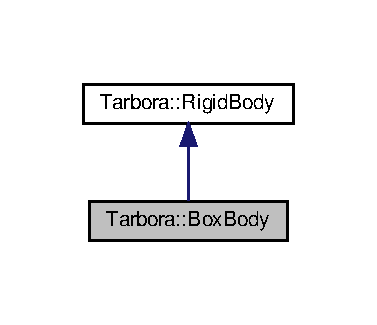
\includegraphics[width=181pt]{classTarbora_1_1BoxBody__inherit__graph}
\end{center}
\end{figure}


Collaboration diagram for Tarbora\+:\+:Box\+Body\+:\nopagebreak
\begin{figure}[H]
\begin{center}
\leavevmode
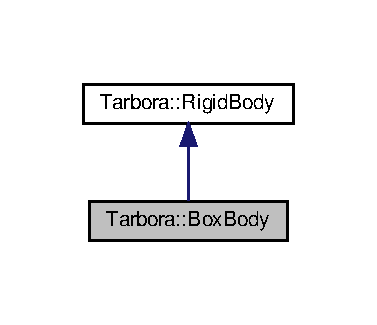
\includegraphics[width=181pt]{classTarbora_1_1BoxBody__coll__graph}
\end{center}
\end{figure}
\subsection*{Public Member Functions}
\begin{DoxyCompactItemize}
\item 
\hyperlink{classTarbora_1_1BoxBody_a4588faa74c221c9f484432bc3b7a0674}{Box\+Body} (glm\+::vec3 \&dimensions)
\begin{DoxyCompactList}\small\item\em Creates a \hyperlink{classTarbora_1_1BoxBody}{Box\+Body}. \end{DoxyCompactList}\item 
\mbox{\Hypertarget{classTarbora_1_1BoxBody_adb0e7074d88a5e14ae8c9abca875ac52}\label{classTarbora_1_1BoxBody_adb0e7074d88a5e14ae8c9abca875ac52}} 
\hyperlink{classTarbora_1_1BoxBody_adb0e7074d88a5e14ae8c9abca875ac52}{$\sim$\+Box\+Body} ()
\begin{DoxyCompactList}\small\item\em Destroys and unregisters this body. \end{DoxyCompactList}\item 
virtual void \hyperlink{classTarbora_1_1BoxBody_a9030e38449087fdf091d9daea5e6efbe}{Register} (unsigned int id, glm\+::mat4 \&transform) override
\begin{DoxyCompactList}\small\item\em Register the rigid body to the Physics Engine. \end{DoxyCompactList}\item 
\mbox{\Hypertarget{classTarbora_1_1BoxBody_a57a94943897a3b90f774935bef82c47c}\label{classTarbora_1_1BoxBody_a57a94943897a3b90f774935bef82c47c}} 
virtual void \hyperlink{classTarbora_1_1BoxBody_a57a94943897a3b90f774935bef82c47c}{Unregister} () override
\begin{DoxyCompactList}\small\item\em Remove the rigid body from the Physics Engine. \end{DoxyCompactList}\item 
\mbox{\Hypertarget{classTarbora_1_1BoxBody_ab5632e04e516e518297a4826c6dd27cb}\label{classTarbora_1_1BoxBody_ab5632e04e516e518297a4826c6dd27cb}} 
virtual void \hyperlink{classTarbora_1_1BoxBody_ab5632e04e516e518297a4826c6dd27cb}{Calc\+Volume} () override
\begin{DoxyCompactList}\small\item\em Calculate the volume when the shape or the size changes. Automatically called by the functions that change those. \end{DoxyCompactList}\item 
void \hyperlink{classTarbora_1_1BoxBody_ae4b822b4acb781e9fdec907e8a92b27b}{Set\+Dimensions} (glm\+::vec3 \&dimensions)
\begin{DoxyCompactList}\small\item\em Set the dimensions of that box, used to calculate the volume and the mass. \end{DoxyCompactList}\item 
\mbox{\Hypertarget{classTarbora_1_1BoxBody_a2c833613435aa7244e39f14460a792c6}\label{classTarbora_1_1BoxBody_a2c833613435aa7244e39f14460a792c6}} 
glm\+::vec3 \& \hyperlink{classTarbora_1_1BoxBody_a2c833613435aa7244e39f14460a792c6}{Get\+Dimensions} ()
\begin{DoxyCompactList}\small\item\em Get the dimensions of that box. \end{DoxyCompactList}\end{DoxyCompactItemize}
\subsection*{Additional Inherited Members}


\subsection{Detailed Description}
A physics rigid body representing a cube. 

\begin{DoxySeeAlso}{See also}
\hyperlink{classTarbora_1_1PhysicsEngine}{Physics\+Engine} 

\hyperlink{classTarbora_1_1RigidBody}{Rigid\+Body} 

\hyperlink{classTarbora_1_1SphereBody}{Sphere\+Body} 
\end{DoxySeeAlso}


\subsection{Constructor \& Destructor Documentation}
\mbox{\Hypertarget{classTarbora_1_1BoxBody_a4588faa74c221c9f484432bc3b7a0674}\label{classTarbora_1_1BoxBody_a4588faa74c221c9f484432bc3b7a0674}} 
\index{Tarbora\+::\+Box\+Body@{Tarbora\+::\+Box\+Body}!Box\+Body@{Box\+Body}}
\index{Box\+Body@{Box\+Body}!Tarbora\+::\+Box\+Body@{Tarbora\+::\+Box\+Body}}
\subsubsection{\texorpdfstring{Box\+Body()}{BoxBody()}}
{\footnotesize\ttfamily Tarbora\+::\+Box\+Body\+::\+Box\+Body (\begin{DoxyParamCaption}\item[{glm\+::vec3 \&}]{dimensions }\end{DoxyParamCaption})}



Creates a \hyperlink{classTarbora_1_1BoxBody}{Box\+Body}. 


\begin{DoxyParams}{Parameters}
{\em dimensions} & A vector representing the dimensions of that box, used to calculate the volume and the mass. \\
\hline
\end{DoxyParams}


\subsection{Member Function Documentation}
\mbox{\Hypertarget{classTarbora_1_1BoxBody_a9030e38449087fdf091d9daea5e6efbe}\label{classTarbora_1_1BoxBody_a9030e38449087fdf091d9daea5e6efbe}} 
\index{Tarbora\+::\+Box\+Body@{Tarbora\+::\+Box\+Body}!Register@{Register}}
\index{Register@{Register}!Tarbora\+::\+Box\+Body@{Tarbora\+::\+Box\+Body}}
\subsubsection{\texorpdfstring{Register()}{Register()}}
{\footnotesize\ttfamily void Tarbora\+::\+Box\+Body\+::\+Register (\begin{DoxyParamCaption}\item[{unsigned int}]{id,  }\item[{glm\+::mat4 \&}]{transform }\end{DoxyParamCaption})\hspace{0.3cm}{\ttfamily [override]}, {\ttfamily [virtual]}}



Register the rigid body to the Physics Engine. 


\begin{DoxyParams}{Parameters}
{\em id} & The id of the actor that owns that rigid body. \\
\hline
{\em transform} & The transform matrix of that actor. \\
\hline
\end{DoxyParams}


Implements \hyperlink{classTarbora_1_1RigidBody_a5f41c214aabe2a7f069a317cb755f0f1}{Tarbora\+::\+Rigid\+Body}.

\mbox{\Hypertarget{classTarbora_1_1BoxBody_ae4b822b4acb781e9fdec907e8a92b27b}\label{classTarbora_1_1BoxBody_ae4b822b4acb781e9fdec907e8a92b27b}} 
\index{Tarbora\+::\+Box\+Body@{Tarbora\+::\+Box\+Body}!Set\+Dimensions@{Set\+Dimensions}}
\index{Set\+Dimensions@{Set\+Dimensions}!Tarbora\+::\+Box\+Body@{Tarbora\+::\+Box\+Body}}
\subsubsection{\texorpdfstring{Set\+Dimensions()}{SetDimensions()}}
{\footnotesize\ttfamily void Tarbora\+::\+Box\+Body\+::\+Set\+Dimensions (\begin{DoxyParamCaption}\item[{glm\+::vec3 \&}]{dimensions }\end{DoxyParamCaption})\hspace{0.3cm}{\ttfamily [inline]}}



Set the dimensions of that box, used to calculate the volume and the mass. 


\begin{DoxyParams}{Parameters}
{\em dimensions} & A vector representing the dimensions of that box. \\
\hline
\end{DoxyParams}


The documentation for this class was generated from the following files\+:\begin{DoxyCompactItemize}
\item 
Tarbora/\+Framework/\+Physics\+Engine/inc/Rigid\+Body.\+hpp\item 
Tarbora/\+Framework/\+Physics\+Engine/src/Rigid\+Body.\+cpp\end{DoxyCompactItemize}

\hypertarget{classTarbora_1_1Camera}{}\section{Tarbora\+:\+:Camera Class Reference}
\label{classTarbora_1_1Camera}\index{Tarbora\+::\+Camera@{Tarbora\+::\+Camera}}


Inheritance diagram for Tarbora\+:\+:Camera\+:\nopagebreak
\begin{figure}[H]
\begin{center}
\leavevmode
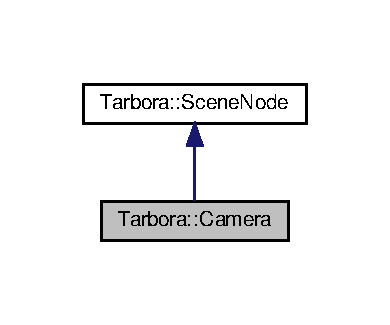
\includegraphics[width=187pt]{classTarbora_1_1Camera__inherit__graph}
\end{center}
\end{figure}


Collaboration diagram for Tarbora\+:\+:Camera\+:\nopagebreak
\begin{figure}[H]
\begin{center}
\leavevmode
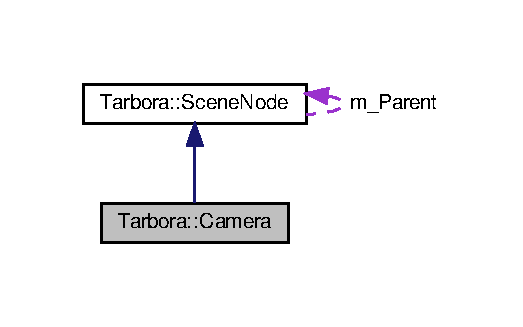
\includegraphics[width=251pt]{classTarbora_1_1Camera__coll__graph}
\end{center}
\end{figure}
\subsection*{Public Member Functions}
\begin{DoxyCompactItemize}
\item 
\mbox{\Hypertarget{classTarbora_1_1Camera_a45153edee036e9ffd270fe4ac4a5067d}\label{classTarbora_1_1Camera_a45153edee036e9ffd270fe4ac4a5067d}} 
{\bfseries Camera} (Actor\+Id actor\+Id, std\+::string name)
\item 
\mbox{\Hypertarget{classTarbora_1_1Camera_a0b29c84c5ac0c00e847c6690bda0ca3a}\label{classTarbora_1_1Camera_a0b29c84c5ac0c00e847c6690bda0ca3a}} 
const glm\+::mat4 {\bfseries Get\+View} ()
\item 
\mbox{\Hypertarget{classTarbora_1_1Camera_a57738b366d754a3657a865b75c23d8fc}\label{classTarbora_1_1Camera_a57738b366d754a3657a865b75c23d8fc}} 
const glm\+::mat4 {\bfseries Get\+View\+Angle} ()
\end{DoxyCompactItemize}
\subsection*{Additional Inherited Members}


The documentation for this class was generated from the following files\+:\begin{DoxyCompactItemize}
\item 
Tarbora/\+Views/\+Graphic\+Views/inc/Scene\+Node.\+hpp\item 
Tarbora/\+Views/\+Graphic\+Views/src/Scene\+Node.\+cpp\end{DoxyCompactItemize}

\hypertarget{classTarbora_1_1CapsuleBody}{}\section{Tarbora\+:\+:Capsule\+Body Class Reference}
\label{classTarbora_1_1CapsuleBody}\index{Tarbora\+::\+Capsule\+Body@{Tarbora\+::\+Capsule\+Body}}


A physics rigid body representing an capsule shape.  




{\ttfamily \#include $<$Rigid\+Body.\+hpp$>$}



Inheritance diagram for Tarbora\+:\+:Capsule\+Body\+:\nopagebreak
\begin{figure}[H]
\begin{center}
\leavevmode
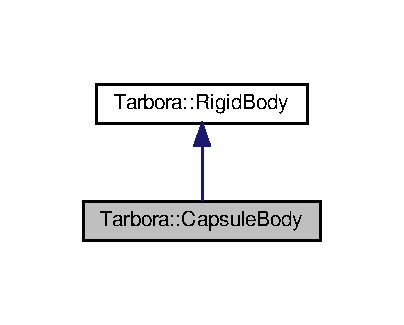
\includegraphics[width=194pt]{classTarbora_1_1CapsuleBody__inherit__graph}
\end{center}
\end{figure}


Collaboration diagram for Tarbora\+:\+:Capsule\+Body\+:\nopagebreak
\begin{figure}[H]
\begin{center}
\leavevmode
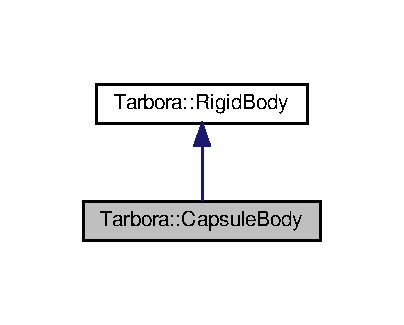
\includegraphics[width=194pt]{classTarbora_1_1CapsuleBody__coll__graph}
\end{center}
\end{figure}
\subsection*{Public Member Functions}
\begin{DoxyCompactItemize}
\item 
\hyperlink{classTarbora_1_1CapsuleBody_ac7427a8fd201d1eb99944d48619e78ed}{Capsule\+Body} (float radius, float height)
\begin{DoxyCompactList}\small\item\em Creates an \hyperlink{classTarbora_1_1CapsuleBody}{Capsule\+Body}. \end{DoxyCompactList}\item 
\mbox{\Hypertarget{classTarbora_1_1CapsuleBody_a70eeff3b16e27269076fef05a42a7de8}\label{classTarbora_1_1CapsuleBody_a70eeff3b16e27269076fef05a42a7de8}} 
\hyperlink{classTarbora_1_1CapsuleBody_a70eeff3b16e27269076fef05a42a7de8}{$\sim$\+Capsule\+Body} ()
\begin{DoxyCompactList}\small\item\em Destroys and unregisters this body. \end{DoxyCompactList}\item 
virtual void \hyperlink{classTarbora_1_1CapsuleBody_a4613a4f0cf0ab92189169d6f3865274e}{register\+Actor} (Actor\+Id \&id, const glm\+::vec3 \&position, const glm\+::quat \&rotation) override
\begin{DoxyCompactList}\small\item\em Register the rigid body to the Physics Engine. \end{DoxyCompactList}\item 
\mbox{\Hypertarget{classTarbora_1_1CapsuleBody_a3cce96469ed469136728ed0ea3004bc0}\label{classTarbora_1_1CapsuleBody_a3cce96469ed469136728ed0ea3004bc0}} 
virtual void \hyperlink{classTarbora_1_1CapsuleBody_a3cce96469ed469136728ed0ea3004bc0}{unregister} () override
\begin{DoxyCompactList}\small\item\em Remove the rigid body from the Physics Engine. \end{DoxyCompactList}\item 
\mbox{\Hypertarget{classTarbora_1_1CapsuleBody_a16af8c987d2a1d6602a317850b0ae17a}\label{classTarbora_1_1CapsuleBody_a16af8c987d2a1d6602a317850b0ae17a}} 
virtual void \hyperlink{classTarbora_1_1CapsuleBody_a16af8c987d2a1d6602a317850b0ae17a}{calc\+Volume} () override
\begin{DoxyCompactList}\small\item\em Calculate the volume when the shape or the size changes. Automatically called by the functions that change those. \end{DoxyCompactList}\item 
void \hyperlink{classTarbora_1_1CapsuleBody_a10ae8b263f437a7d810f727cd7e7e943}{set\+Radius} (float radius)
\begin{DoxyCompactList}\small\item\em Set the radius of that capsule. \end{DoxyCompactList}\item 
\mbox{\Hypertarget{classTarbora_1_1CapsuleBody_a3c4217bfdf918f48a49221e07aee262c}\label{classTarbora_1_1CapsuleBody_a3c4217bfdf918f48a49221e07aee262c}} 
float \hyperlink{classTarbora_1_1CapsuleBody_a3c4217bfdf918f48a49221e07aee262c}{get\+Radius} ()
\begin{DoxyCompactList}\small\item\em Get the radius of that sphere. \end{DoxyCompactList}\item 
void \hyperlink{classTarbora_1_1CapsuleBody_a8ecfb8196d5156649b8e04256e1d63c1}{set\+Height} (float height)
\begin{DoxyCompactList}\small\item\em Set the height of that capsule. \end{DoxyCompactList}\item 
\mbox{\Hypertarget{classTarbora_1_1CapsuleBody_a521b8b538755f1f72c7298a4a291053d}\label{classTarbora_1_1CapsuleBody_a521b8b538755f1f72c7298a4a291053d}} 
float \hyperlink{classTarbora_1_1CapsuleBody_a521b8b538755f1f72c7298a4a291053d}{get\+Height} ()
\begin{DoxyCompactList}\small\item\em Get the height of that sphere. \end{DoxyCompactList}\end{DoxyCompactItemize}
\subsection*{Additional Inherited Members}


\subsection{Detailed Description}
A physics rigid body representing an capsule shape. 

\begin{DoxySeeAlso}{See also}
\hyperlink{classTarbora_1_1PhysicsEngine}{Physics\+Engine} 

\hyperlink{classTarbora_1_1RigidBody}{Rigid\+Body} 

\hyperlink{classTarbora_1_1SphereBody}{Sphere\+Body} 
\end{DoxySeeAlso}


\subsection{Constructor \& Destructor Documentation}
\mbox{\Hypertarget{classTarbora_1_1CapsuleBody_ac7427a8fd201d1eb99944d48619e78ed}\label{classTarbora_1_1CapsuleBody_ac7427a8fd201d1eb99944d48619e78ed}} 
\index{Tarbora\+::\+Capsule\+Body@{Tarbora\+::\+Capsule\+Body}!Capsule\+Body@{Capsule\+Body}}
\index{Capsule\+Body@{Capsule\+Body}!Tarbora\+::\+Capsule\+Body@{Tarbora\+::\+Capsule\+Body}}
\subsubsection{\texorpdfstring{Capsule\+Body()}{CapsuleBody()}}
{\footnotesize\ttfamily Tarbora\+::\+Capsule\+Body\+::\+Capsule\+Body (\begin{DoxyParamCaption}\item[{float}]{radius,  }\item[{float}]{height }\end{DoxyParamCaption})}



Creates an \hyperlink{classTarbora_1_1CapsuleBody}{Capsule\+Body}. 


\begin{DoxyParams}{Parameters}
{\em radius} & The radius of that capsule, used to calculate the volume and the mass. \\
\hline
{\em height} & The height of that capsule, used to calculate the volume and the mass. \\
\hline
\end{DoxyParams}


\subsection{Member Function Documentation}
\mbox{\Hypertarget{classTarbora_1_1CapsuleBody_a4613a4f0cf0ab92189169d6f3865274e}\label{classTarbora_1_1CapsuleBody_a4613a4f0cf0ab92189169d6f3865274e}} 
\index{Tarbora\+::\+Capsule\+Body@{Tarbora\+::\+Capsule\+Body}!register\+Actor@{register\+Actor}}
\index{register\+Actor@{register\+Actor}!Tarbora\+::\+Capsule\+Body@{Tarbora\+::\+Capsule\+Body}}
\subsubsection{\texorpdfstring{register\+Actor()}{registerActor()}}
{\footnotesize\ttfamily void Tarbora\+::\+Capsule\+Body\+::register\+Actor (\begin{DoxyParamCaption}\item[{Actor\+Id \&}]{id,  }\item[{const glm\+::vec3 \&}]{position,  }\item[{const glm\+::quat \&}]{rotation }\end{DoxyParamCaption})\hspace{0.3cm}{\ttfamily [override]}, {\ttfamily [virtual]}}



Register the rigid body to the Physics Engine. 


\begin{DoxyParams}{Parameters}
{\em id} & The id of the actor that owns that rigid body. \\
\hline
{\em position} & The initial position of that actor. \\
\hline
{\em rotation} & The initial rotation of that actor. \\
\hline
\end{DoxyParams}


Implements \hyperlink{classTarbora_1_1RigidBody_acd1c63e93fd607f74f48fb68aa764b29}{Tarbora\+::\+Rigid\+Body}.

\mbox{\Hypertarget{classTarbora_1_1CapsuleBody_a8ecfb8196d5156649b8e04256e1d63c1}\label{classTarbora_1_1CapsuleBody_a8ecfb8196d5156649b8e04256e1d63c1}} 
\index{Tarbora\+::\+Capsule\+Body@{Tarbora\+::\+Capsule\+Body}!set\+Height@{set\+Height}}
\index{set\+Height@{set\+Height}!Tarbora\+::\+Capsule\+Body@{Tarbora\+::\+Capsule\+Body}}
\subsubsection{\texorpdfstring{set\+Height()}{setHeight()}}
{\footnotesize\ttfamily void Tarbora\+::\+Capsule\+Body\+::set\+Height (\begin{DoxyParamCaption}\item[{float}]{height }\end{DoxyParamCaption})\hspace{0.3cm}{\ttfamily [inline]}}



Set the height of that capsule. 


\begin{DoxyParams}{Parameters}
{\em height} & The height of that capsule, used to calculate the volume and the mass. \\
\hline
\end{DoxyParams}
\mbox{\Hypertarget{classTarbora_1_1CapsuleBody_a10ae8b263f437a7d810f727cd7e7e943}\label{classTarbora_1_1CapsuleBody_a10ae8b263f437a7d810f727cd7e7e943}} 
\index{Tarbora\+::\+Capsule\+Body@{Tarbora\+::\+Capsule\+Body}!set\+Radius@{set\+Radius}}
\index{set\+Radius@{set\+Radius}!Tarbora\+::\+Capsule\+Body@{Tarbora\+::\+Capsule\+Body}}
\subsubsection{\texorpdfstring{set\+Radius()}{setRadius()}}
{\footnotesize\ttfamily void Tarbora\+::\+Capsule\+Body\+::set\+Radius (\begin{DoxyParamCaption}\item[{float}]{radius }\end{DoxyParamCaption})\hspace{0.3cm}{\ttfamily [inline]}}



Set the radius of that capsule. 


\begin{DoxyParams}{Parameters}
{\em radius} & The radius of that capsule, used to calculate the volume and the mass. \\
\hline
\end{DoxyParams}


The documentation for this class was generated from the following files\+:\begin{DoxyCompactItemize}
\item 
Tarbora/\+Logic/\+Physics\+Engine/Rigid\+Body.\+hpp\item 
Tarbora/\+Logic/\+Physics\+Engine/Rigid\+Body.\+cpp\end{DoxyCompactItemize}

\hypertarget{classTarbora_1_1Component}{}\section{Tarbora\+:\+:Component Class Reference}
\label{classTarbora_1_1Component}\index{Tarbora\+::\+Component@{Tarbora\+::\+Component}}


Inheritance diagram for Tarbora\+:\+:Component\+:
\nopagebreak
\begin{figure}[H]
\begin{center}
\leavevmode
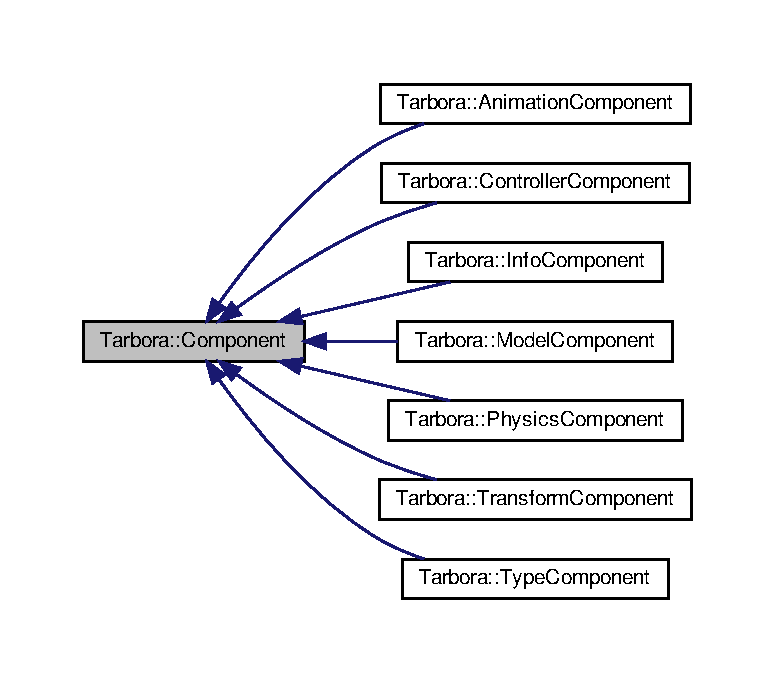
\includegraphics[width=350pt]{classTarbora_1_1Component__inherit__graph}
\end{center}
\end{figure}


Collaboration diagram for Tarbora\+:\+:Component\+:
\nopagebreak
\begin{figure}[H]
\begin{center}
\leavevmode
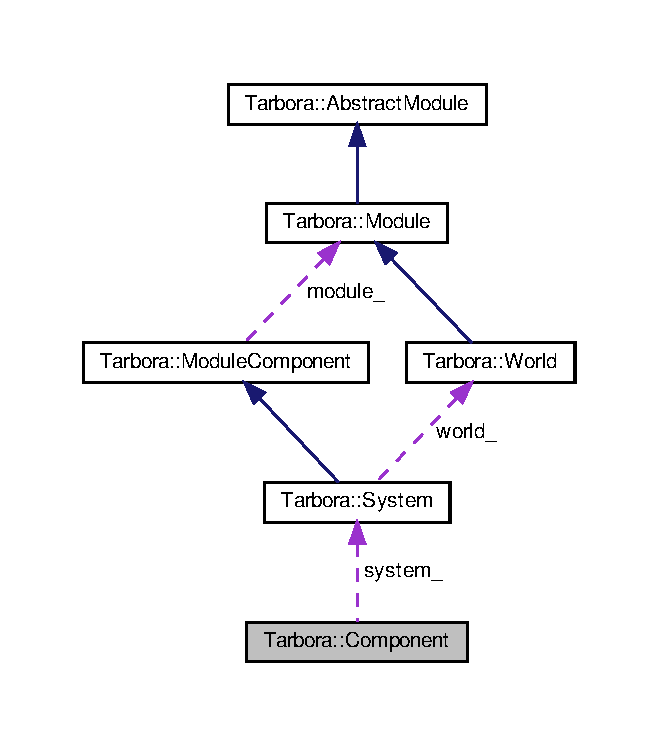
\includegraphics[width=316pt]{classTarbora_1_1Component__coll__graph}
\end{center}
\end{figure}
\subsection*{Public Member Functions}
\begin{DoxyCompactItemize}
\item 
\mbox{\Hypertarget{classTarbora_1_1Component_af131ce04afe7eadb2589afcec5fa52d8}\label{classTarbora_1_1Component_af131ce04afe7eadb2589afcec5fa52d8}} 
{\bfseries Component} (\hyperlink{classTarbora_1_1System}{System} $\ast$s, const Actor\+Id \&id, const \hyperlink{classTarbora_1_1LuaTable}{Lua\+Table} \&table)
\item 
\mbox{\Hypertarget{classTarbora_1_1Component_a9b772f4d99f64b23685a58e7294ab981}\label{classTarbora_1_1Component_a9b772f4d99f64b23685a58e7294ab981}} 
\hyperlink{classTarbora_1_1Component}{Component} $\ast$ {\bfseries get\+Component} (const Actor\+Id \&id, const Component\+Id \&component)
\item 
\mbox{\Hypertarget{classTarbora_1_1Component_abeeb3dba77af922915cbe9bc7d29d646}\label{classTarbora_1_1Component_abeeb3dba77af922915cbe9bc7d29d646}} 
\hyperlink{classTarbora_1_1Component}{Component} $\ast$ {\bfseries get\+Component} (const Component\+Id \&component)
\item 
\mbox{\Hypertarget{classTarbora_1_1Component_a856a0b9e17ccd0336f1a33cf2fd2ac20}\label{classTarbora_1_1Component_a856a0b9e17ccd0336f1a33cf2fd2ac20}} 
void {\bfseries enable} ()
\item 
\mbox{\Hypertarget{classTarbora_1_1Component_a163aa5702b50ede0dddfe1f8620afca5}\label{classTarbora_1_1Component_a163aa5702b50ede0dddfe1f8620afca5}} 
void {\bfseries disable} ()
\item 
\mbox{\Hypertarget{classTarbora_1_1Component_a227a558106b74d4b8b0be7667c7610c5}\label{classTarbora_1_1Component_a227a558106b74d4b8b0be7667c7610c5}} 
void {\bfseries send} (Client\+Id to, Message\+Subject s, \hyperlink{classTarbora_1_1MessageBody}{Message\+Body} b) const
\item 
\mbox{\Hypertarget{classTarbora_1_1Component_a47985733836fce6b3cc5e0f77607d4e8}\label{classTarbora_1_1Component_a47985733836fce6b3cc5e0f77607d4e8}} 
void {\bfseries trigger} (Message\+Subject s, \hyperlink{classTarbora_1_1MessageBody}{Message\+Body} b) const
\item 
\mbox{\Hypertarget{classTarbora_1_1Component_aa3eddb1cf4ba3fb1f0652d0c3aee07b6}\label{classTarbora_1_1Component_aa3eddb1cf4ba3fb1f0652d0c3aee07b6}} 
void {\bfseries trigger\+Local} (Message\+Subject s, \hyperlink{classTarbora_1_1MessageBody}{Message\+Body} b) const
\item 
\mbox{\Hypertarget{classTarbora_1_1Component_ad8232ed039bec74c81fc7589ee34cbf7}\label{classTarbora_1_1Component_ad8232ed039bec74c81fc7589ee34cbf7}} 
bool {\bfseries error} ()
\end{DoxyCompactItemize}
\subsection*{Protected Member Functions}
\begin{DoxyCompactItemize}
\item 
\mbox{\Hypertarget{classTarbora_1_1Component_a644061cabaf91ed54eae79ce616c25b9}\label{classTarbora_1_1Component_a644061cabaf91ed54eae79ce616c25b9}} 
virtual void {\bfseries on\+Enable} ()
\item 
\mbox{\Hypertarget{classTarbora_1_1Component_a62150a85e0eb8f3601d211245ca08a2d}\label{classTarbora_1_1Component_a62150a85e0eb8f3601d211245ca08a2d}} 
virtual void {\bfseries on\+Disable} ()
\end{DoxyCompactItemize}
\subsection*{Protected Attributes}
\begin{DoxyCompactItemize}
\item 
\mbox{\Hypertarget{classTarbora_1_1Component_a19bde335970f5e3af9bc845122f28f3f}\label{classTarbora_1_1Component_a19bde335970f5e3af9bc845122f28f3f}} 
\hyperlink{classTarbora_1_1System}{System} $\ast$ {\bfseries system\+\_\+}
\item 
\mbox{\Hypertarget{classTarbora_1_1Component_a4c2092ce4a44d193308669024867775c}\label{classTarbora_1_1Component_a4c2092ce4a44d193308669024867775c}} 
Actor\+Id {\bfseries owner\+\_\+}
\item 
\mbox{\Hypertarget{classTarbora_1_1Component_ac5b26f24609f28419cf2a2e6065b17c8}\label{classTarbora_1_1Component_ac5b26f24609f28419cf2a2e6065b17c8}} 
bool {\bfseries enabled\+\_\+}
\item 
\mbox{\Hypertarget{classTarbora_1_1Component_a7e022fe62bcf3c3781977ca972383c0d}\label{classTarbora_1_1Component_a7e022fe62bcf3c3781977ca972383c0d}} 
bool {\bfseries error\+\_\+}
\end{DoxyCompactItemize}


The documentation for this class was generated from the following file\+:\begin{DoxyCompactItemize}
\item 
Tarbora/\+Logic/Component.\+hpp\end{DoxyCompactItemize}

\hypertarget{classTarbora_1_1ControllerComponent}{}\section{Tarbora\+:\+:Controller\+Component Class Reference}
\label{classTarbora_1_1ControllerComponent}\index{Tarbora\+::\+Controller\+Component@{Tarbora\+::\+Controller\+Component}}


Inheritance diagram for Tarbora\+:\+:Controller\+Component\+:
\nopagebreak
\begin{figure}[H]
\begin{center}
\leavevmode
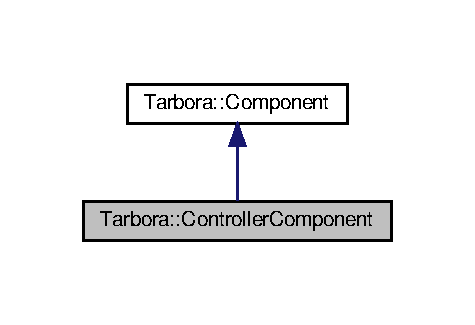
\includegraphics[width=228pt]{classTarbora_1_1ControllerComponent__inherit__graph}
\end{center}
\end{figure}


Collaboration diagram for Tarbora\+:\+:Controller\+Component\+:
\nopagebreak
\begin{figure}[H]
\begin{center}
\leavevmode
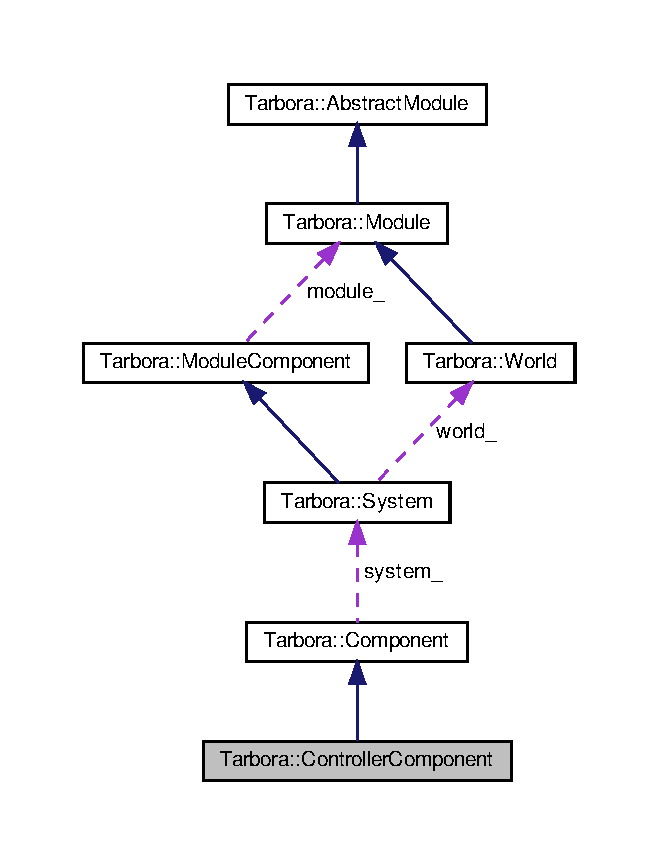
\includegraphics[width=316pt]{classTarbora_1_1ControllerComponent__coll__graph}
\end{center}
\end{figure}
\subsection*{Public Member Functions}
\begin{DoxyCompactItemize}
\item 
\mbox{\Hypertarget{classTarbora_1_1ControllerComponent_a87e3acf975ce4c3950b24b0063b12736}\label{classTarbora_1_1ControllerComponent_a87e3acf975ce4c3950b24b0063b12736}} 
{\bfseries Controller\+Component} (\hyperlink{classTarbora_1_1System}{System} $\ast$s, const Actor\+Id \&id, const \hyperlink{classTarbora_1_1LuaTable}{Lua\+Table} \&table)
\item 
\mbox{\Hypertarget{classTarbora_1_1ControllerComponent_aa344a1b82231c93df1b09ad730928a69}\label{classTarbora_1_1ControllerComponent_aa344a1b82231c93df1b09ad730928a69}} 
void {\bfseries set\+Movement} (const glm\+::vec3 \&direction)
\item 
\mbox{\Hypertarget{classTarbora_1_1ControllerComponent_ab05aa76636b3fe81b19d600d67cedb10}\label{classTarbora_1_1ControllerComponent_ab05aa76636b3fe81b19d600d67cedb10}} 
void {\bfseries set\+Look\+Direction} (const glm\+::vec3 \&direction)
\end{DoxyCompactItemize}
\subsection*{Friends}
\begin{DoxyCompactItemize}
\item 
\mbox{\Hypertarget{classTarbora_1_1ControllerComponent_aa3529c8d40124ce67f4463a28e41118c}\label{classTarbora_1_1ControllerComponent_aa3529c8d40124ce67f4463a28e41118c}} 
class {\bfseries Controller\+System}
\end{DoxyCompactItemize}
\subsection*{Additional Inherited Members}


The documentation for this class was generated from the following files\+:\begin{DoxyCompactItemize}
\item 
Tarbora/\+Logic/Controller\+Component.\+hpp\item 
Tarbora/\+Logic/Controller\+Component.\+cpp\end{DoxyCompactItemize}

\hypertarget{classTarbora_1_1ControllerSystem}{}\section{Tarbora\+:\+:Controller\+System Class Reference}
\label{classTarbora_1_1ControllerSystem}\index{Tarbora\+::\+Controller\+System@{Tarbora\+::\+Controller\+System}}


Inheritance diagram for Tarbora\+:\+:Controller\+System\+:\nopagebreak
\begin{figure}[H]
\begin{center}
\leavevmode
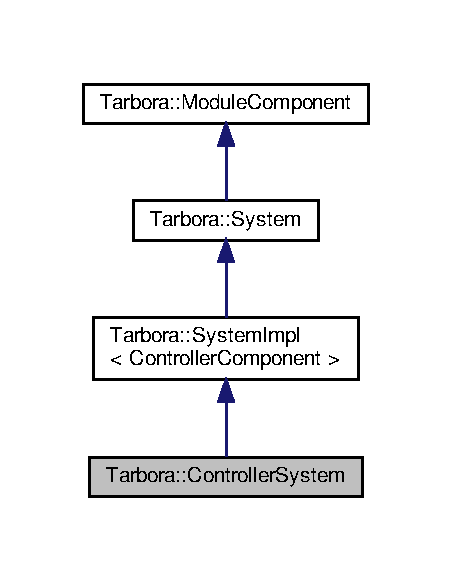
\includegraphics[width=217pt]{classTarbora_1_1ControllerSystem__inherit__graph}
\end{center}
\end{figure}


Collaboration diagram for Tarbora\+:\+:Controller\+System\+:\nopagebreak
\begin{figure}[H]
\begin{center}
\leavevmode
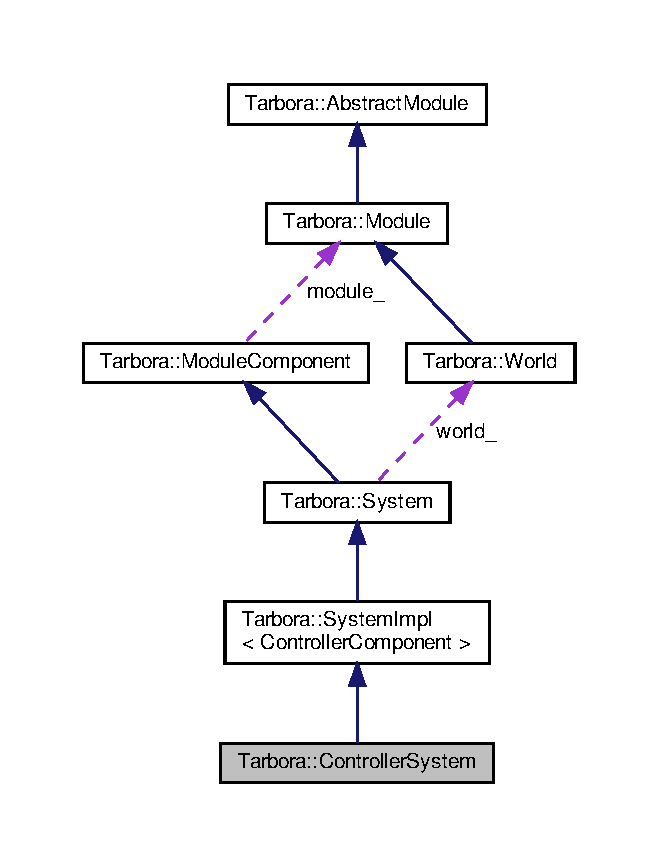
\includegraphics[width=316pt]{classTarbora_1_1ControllerSystem__coll__graph}
\end{center}
\end{figure}
\subsection*{Public Member Functions}
\begin{DoxyCompactItemize}
\item 
\mbox{\Hypertarget{classTarbora_1_1ControllerSystem_af2f2f8df2b467fb113fdcc38c48784e8}\label{classTarbora_1_1ControllerSystem_af2f2f8df2b467fb113fdcc38c48784e8}} 
{\bfseries Controller\+System} (\hyperlink{classTarbora_1_1World}{World} $\ast$w)
\item 
\mbox{\Hypertarget{classTarbora_1_1ControllerSystem_ac117af8c62be21fe5bf9188b32606009}\label{classTarbora_1_1ControllerSystem_ac117af8c62be21fe5bf9188b32606009}} 
virtual void {\bfseries init} (const Actor\+Id \&id)
\item 
\mbox{\Hypertarget{classTarbora_1_1ControllerSystem_a3798b5b50d140e986a6cfc1b4467bc7b}\label{classTarbora_1_1ControllerSystem_a3798b5b50d140e986a6cfc1b4467bc7b}} 
virtual void {\bfseries update} (float delta\+\_\+time)
\end{DoxyCompactItemize}
\subsection*{Static Public Member Functions}
\begin{DoxyCompactItemize}
\item 
\mbox{\Hypertarget{classTarbora_1_1ControllerSystem_adca814b261e48d028367dffab874ed5e}\label{classTarbora_1_1ControllerSystem_adca814b261e48d028367dffab874ed5e}} 
static std\+::string {\bfseries get\+Name} ()
\end{DoxyCompactItemize}
\subsection*{Additional Inherited Members}


The documentation for this class was generated from the following files\+:\begin{DoxyCompactItemize}
\item 
Tarbora/\+Logic/Controller\+Component.\+hpp\item 
Tarbora/\+Logic/Controller\+Component.\+cpp\end{DoxyCompactItemize}

\hypertarget{classTarbora_1_1Message_1_1CreateActor}{}\section{Tarbora\+:\+:Message\+:\+:Create\+Actor Class Reference}
\label{classTarbora_1_1Message_1_1CreateActor}\index{Tarbora\+::\+Message\+::\+Create\+Actor@{Tarbora\+::\+Message\+::\+Create\+Actor}}


Inheritance diagram for Tarbora\+:\+:Message\+:\+:Create\+Actor\+:\nopagebreak
\begin{figure}[H]
\begin{center}
\leavevmode
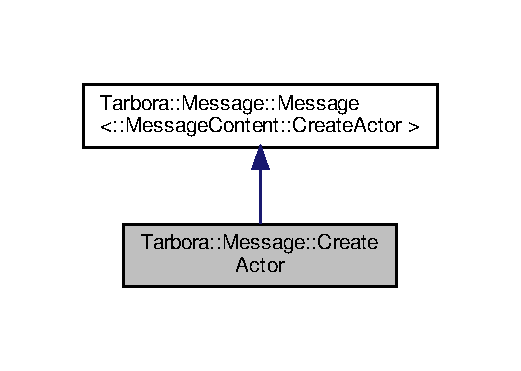
\includegraphics[width=250pt]{classTarbora_1_1Message_1_1CreateActor__inherit__graph}
\end{center}
\end{figure}


Collaboration diagram for Tarbora\+:\+:Message\+:\+:Create\+Actor\+:\nopagebreak
\begin{figure}[H]
\begin{center}
\leavevmode
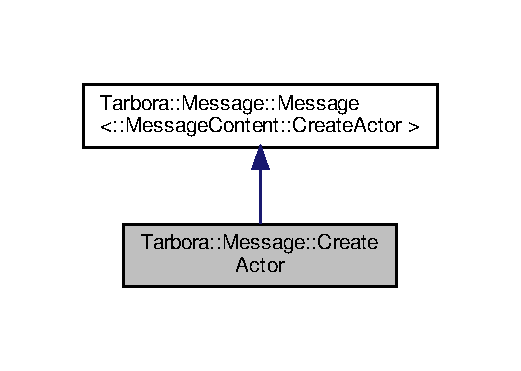
\includegraphics[width=250pt]{classTarbora_1_1Message_1_1CreateActor__coll__graph}
\end{center}
\end{figure}
\subsection*{Public Member Functions}
\begin{DoxyCompactItemize}
\item 
\mbox{\Hypertarget{classTarbora_1_1Message_1_1CreateActor_a501ffd356544e55a1b9fb4e6f7620259}\label{classTarbora_1_1Message_1_1CreateActor_a501ffd356544e55a1b9fb4e6f7620259}} 
{\bfseries Create\+Actor} (const \hyperlink{classTarbora_1_1MessageBody}{Message\+Body} \&m)
\item 
\mbox{\Hypertarget{classTarbora_1_1Message_1_1CreateActor_a21f3d9d4de2508519868d6b7db21e1a5}\label{classTarbora_1_1Message_1_1CreateActor_a21f3d9d4de2508519868d6b7db21e1a5}} 
{\bfseries Create\+Actor} (const Actor\+Id \&id, const std\+::string \&entity, const std\+::string \&variant)
\item 
\mbox{\Hypertarget{classTarbora_1_1Message_1_1CreateActor_a19ba27e4e49e3c3546ece8abedd02649}\label{classTarbora_1_1Message_1_1CreateActor_a19ba27e4e49e3c3546ece8abedd02649}} 
{\bfseries Create\+Actor} (const Actor\+Id \&id, const std\+::string \&entity, const std\+::string \&variant, const glm\+::vec3 \&position)
\item 
\mbox{\Hypertarget{classTarbora_1_1Message_1_1CreateActor_a61b1b77a3ee2eccd9b2938db1a6804ad}\label{classTarbora_1_1Message_1_1CreateActor_a61b1b77a3ee2eccd9b2938db1a6804ad}} 
{\bfseries Create\+Actor} (const Actor\+Id \&id, const std\+::string \&entity, const std\+::string \&variant, const glm\+::quat \&rotation)
\item 
\mbox{\Hypertarget{classTarbora_1_1Message_1_1CreateActor_a8e1d258d129e43403dacf00939cf19ea}\label{classTarbora_1_1Message_1_1CreateActor_a8e1d258d129e43403dacf00939cf19ea}} 
{\bfseries Create\+Actor} (const Actor\+Id \&id, const std\+::string \&entity, const std\+::string \&variant, const glm\+::vec3 \&position, const glm\+::quat \&rotation)
\item 
\mbox{\Hypertarget{classTarbora_1_1Message_1_1CreateActor_a945d190ee49b62ad72ea6a42874d924a}\label{classTarbora_1_1Message_1_1CreateActor_a945d190ee49b62ad72ea6a42874d924a}} 
const Actor\+Id \& {\bfseries get\+Id} ()
\item 
\mbox{\Hypertarget{classTarbora_1_1Message_1_1CreateActor_a8afc9f7695e460c7307154509841c77a}\label{classTarbora_1_1Message_1_1CreateActor_a8afc9f7695e460c7307154509841c77a}} 
const std\+::string \& {\bfseries get\+Entity} ()
\item 
\mbox{\Hypertarget{classTarbora_1_1Message_1_1CreateActor_aa4ae5b20c334a946846bfbbf3dabde96}\label{classTarbora_1_1Message_1_1CreateActor_aa4ae5b20c334a946846bfbbf3dabde96}} 
const std\+::string \& {\bfseries get\+Variant} ()
\item 
\mbox{\Hypertarget{classTarbora_1_1Message_1_1CreateActor_ada9e16bb08abadaf245c4993a8a588dc}\label{classTarbora_1_1Message_1_1CreateActor_ada9e16bb08abadaf245c4993a8a588dc}} 
glm\+::vec3 {\bfseries get\+Position} ()
\item 
\mbox{\Hypertarget{classTarbora_1_1Message_1_1CreateActor_af7068fa52473ad3592038af0f8492905}\label{classTarbora_1_1Message_1_1CreateActor_af7068fa52473ad3592038af0f8492905}} 
glm\+::quat {\bfseries get\+Rotation} ()
\item 
\mbox{\Hypertarget{classTarbora_1_1Message_1_1CreateActor_acf1b3e888fd715357d59e697e0d25caa}\label{classTarbora_1_1Message_1_1CreateActor_acf1b3e888fd715357d59e697e0d25caa}} 
bool {\bfseries has\+Position} ()
\item 
\mbox{\Hypertarget{classTarbora_1_1Message_1_1CreateActor_a073fd44432d7db362801497af7af31d7}\label{classTarbora_1_1Message_1_1CreateActor_a073fd44432d7db362801497af7af31d7}} 
bool {\bfseries has\+Rotation} ()
\end{DoxyCompactItemize}
\subsection*{Additional Inherited Members}


The documentation for this class was generated from the following files\+:\begin{DoxyCompactItemize}
\item 
Tarbora/\+Messages/Basic\+Messages.\+hpp\item 
Tarbora/\+Messages/Basic\+Messages.\+cpp\end{DoxyCompactItemize}

\hypertarget{classTarbora_1_1Message_1_1CreateActorModel}{}\section{Tarbora\+:\+:Message\+:\+:Create\+Actor\+Model Class Reference}
\label{classTarbora_1_1Message_1_1CreateActorModel}\index{Tarbora\+::\+Message\+::\+Create\+Actor\+Model@{Tarbora\+::\+Message\+::\+Create\+Actor\+Model}}


Inheritance diagram for Tarbora\+:\+:Message\+:\+:Create\+Actor\+Model\+:\nopagebreak
\begin{figure}[H]
\begin{center}
\leavevmode
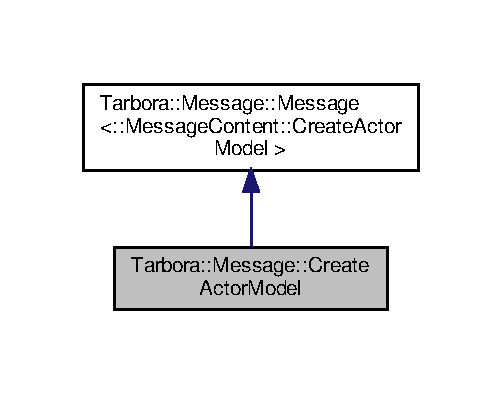
\includegraphics[width=241pt]{classTarbora_1_1Message_1_1CreateActorModel__inherit__graph}
\end{center}
\end{figure}


Collaboration diagram for Tarbora\+:\+:Message\+:\+:Create\+Actor\+Model\+:\nopagebreak
\begin{figure}[H]
\begin{center}
\leavevmode
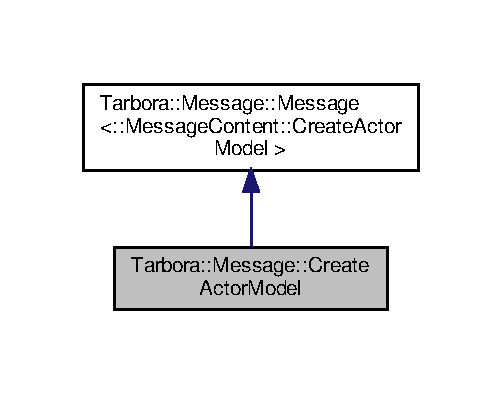
\includegraphics[width=241pt]{classTarbora_1_1Message_1_1CreateActorModel__coll__graph}
\end{center}
\end{figure}
\subsection*{Public Member Functions}
\begin{DoxyCompactItemize}
\item 
\mbox{\Hypertarget{classTarbora_1_1Message_1_1CreateActorModel_aaca323d57bb2307b5a381eb901918c7c}\label{classTarbora_1_1Message_1_1CreateActorModel_aaca323d57bb2307b5a381eb901918c7c}} 
{\bfseries Create\+Actor\+Model} (const \hyperlink{classTarbora_1_1MessageBody}{Message\+Body} \&m)
\item 
\mbox{\Hypertarget{classTarbora_1_1Message_1_1CreateActorModel_a1567478f4fa8904cba8290ba707d67d1}\label{classTarbora_1_1Message_1_1CreateActorModel_a1567478f4fa8904cba8290ba707d67d1}} 
{\bfseries Create\+Actor\+Model} (const Actor\+Id \&id, const std\+::string \&model, const std\+::string \&material, int render\+\_\+pass)
\item 
\mbox{\Hypertarget{classTarbora_1_1Message_1_1CreateActorModel_ad513b7047d839b117131614dfef36981}\label{classTarbora_1_1Message_1_1CreateActorModel_ad513b7047d839b117131614dfef36981}} 
const Actor\+Id \& {\bfseries get\+Id} ()
\item 
\mbox{\Hypertarget{classTarbora_1_1Message_1_1CreateActorModel_a472e819af3b414744a3036a15bc5b5e9}\label{classTarbora_1_1Message_1_1CreateActorModel_a472e819af3b414744a3036a15bc5b5e9}} 
const std\+::string \& {\bfseries get\+Model} ()
\item 
\mbox{\Hypertarget{classTarbora_1_1Message_1_1CreateActorModel_ac7d8f3762505744d6f0ee5f2f2ca9340}\label{classTarbora_1_1Message_1_1CreateActorModel_ac7d8f3762505744d6f0ee5f2f2ca9340}} 
const std\+::string \& {\bfseries get\+Material} ()
\item 
\mbox{\Hypertarget{classTarbora_1_1Message_1_1CreateActorModel_a3654fdadb01c5449c069aa2c02e111c8}\label{classTarbora_1_1Message_1_1CreateActorModel_a3654fdadb01c5449c069aa2c02e111c8}} 
int {\bfseries get\+Render\+Pass} ()
\end{DoxyCompactItemize}
\subsection*{Additional Inherited Members}


The documentation for this class was generated from the following file\+:\begin{DoxyCompactItemize}
\item 
Tarbora/\+Messages/Basic\+Messages.\+hpp\end{DoxyCompactItemize}

\hypertarget{classTarbora_1_1DemoWindow}{}\section{Tarbora\+:\+:Demo\+Window Class Reference}
\label{classTarbora_1_1DemoWindow}\index{Tarbora\+::\+Demo\+Window@{Tarbora\+::\+Demo\+Window}}


Inheritance diagram for Tarbora\+:\+:Demo\+Window\+:
\nopagebreak
\begin{figure}[H]
\begin{center}
\leavevmode
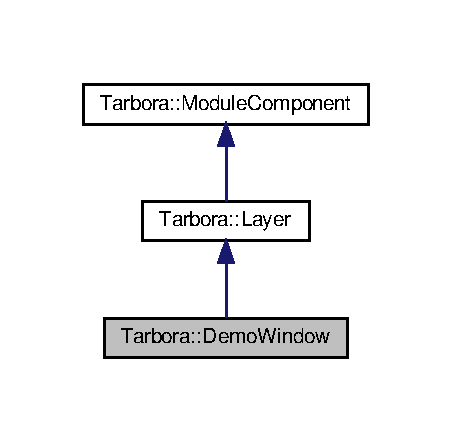
\includegraphics[width=217pt]{classTarbora_1_1DemoWindow__inherit__graph}
\end{center}
\end{figure}


Collaboration diagram for Tarbora\+:\+:Demo\+Window\+:
\nopagebreak
\begin{figure}[H]
\begin{center}
\leavevmode
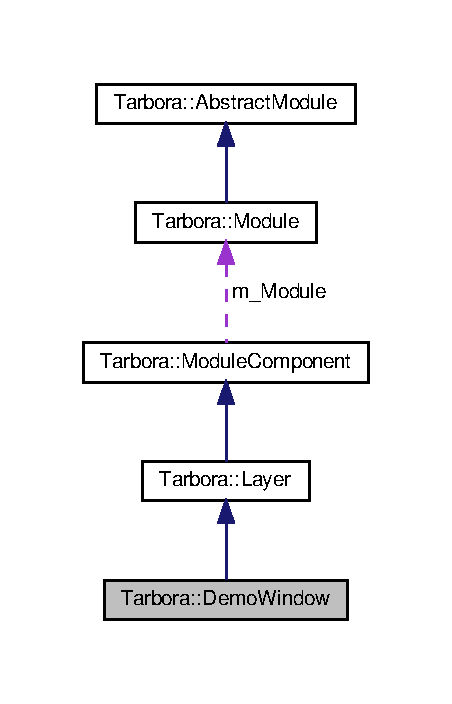
\includegraphics[width=217pt]{classTarbora_1_1DemoWindow__coll__graph}
\end{center}
\end{figure}
\subsection*{Public Member Functions}
\begin{DoxyCompactItemize}
\item 
\mbox{\Hypertarget{classTarbora_1_1DemoWindow_a20c62ad3f1602152c50efcb1e2c3b16d}\label{classTarbora_1_1DemoWindow_a20c62ad3f1602152c50efcb1e2c3b16d}} 
{\bfseries Demo\+Window} (\hyperlink{classTarbora_1_1GraphicView}{Graphic\+View} $\ast$view, bool start\+\_\+active)
\item 
\mbox{\Hypertarget{classTarbora_1_1DemoWindow_a8537497b035002c4adcf3c2ab97069f1}\label{classTarbora_1_1DemoWindow_a8537497b035002c4adcf3c2ab97069f1}} 
void {\bfseries get\+Input} () override
\item 
\mbox{\Hypertarget{classTarbora_1_1DemoWindow_a88b0354686e440a7bd783ccf33dafe6a}\label{classTarbora_1_1DemoWindow_a88b0354686e440a7bd783ccf33dafe6a}} 
void {\bfseries draw} () override
\end{DoxyCompactItemize}
\subsection*{Additional Inherited Members}


The documentation for this class was generated from the following file\+:\begin{DoxyCompactItemize}
\item 
Tarbora/\+Views/\+Graphic\+Views/Demo\+Window.\+hpp\end{DoxyCompactItemize}

\hypertarget{classTarbora_1_1Editor}{}\section{Tarbora\+:\+:Editor Class Reference}
\label{classTarbora_1_1Editor}\index{Tarbora\+::\+Editor@{Tarbora\+::\+Editor}}


Inheritance diagram for Tarbora\+:\+:Editor\+:\nopagebreak
\begin{figure}[H]
\begin{center}
\leavevmode
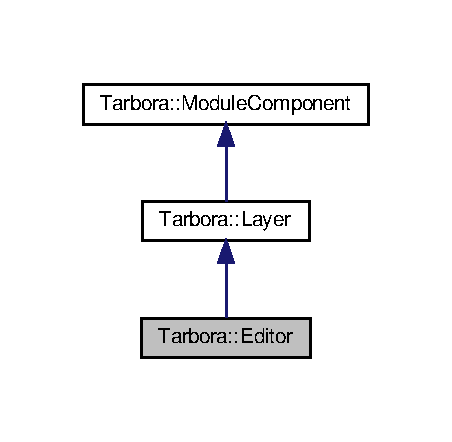
\includegraphics[width=217pt]{classTarbora_1_1Editor__inherit__graph}
\end{center}
\end{figure}


Collaboration diagram for Tarbora\+:\+:Editor\+:\nopagebreak
\begin{figure}[H]
\begin{center}
\leavevmode
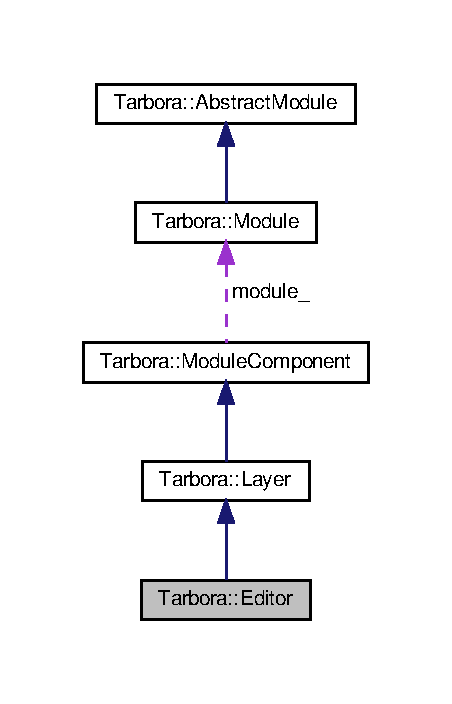
\includegraphics[width=217pt]{classTarbora_1_1Editor__coll__graph}
\end{center}
\end{figure}
\subsection*{Public Member Functions}
\begin{DoxyCompactItemize}
\item 
\mbox{\Hypertarget{classTarbora_1_1Editor_a18df23a4933529187d0be5b5ed888d15}\label{classTarbora_1_1Editor_a18df23a4933529187d0be5b5ed888d15}} 
{\bfseries Editor} (\hyperlink{classTarbora_1_1HumanView}{Human\+View} $\ast$view, bool start\+Active)
\item 
\mbox{\Hypertarget{classTarbora_1_1Editor_abda8f6310f84da26b10e421e16824ca7}\label{classTarbora_1_1Editor_abda8f6310f84da26b10e421e16824ca7}} 
virtual void {\bfseries get\+Input} ()
\item 
\mbox{\Hypertarget{classTarbora_1_1Editor_a12c8f8675b4745e6a303ea1b6132766c}\label{classTarbora_1_1Editor_a12c8f8675b4745e6a303ea1b6132766c}} 
virtual void {\bfseries draw} ()
\end{DoxyCompactItemize}
\subsection*{Public Attributes}
\begin{DoxyCompactItemize}
\item 
\mbox{\Hypertarget{classTarbora_1_1Editor_a044526f8e2770401422709dc275f8bc2}\label{classTarbora_1_1Editor_a044526f8e2770401422709dc275f8bc2}} 
std\+::shared\+\_\+ptr$<$ \hyperlink{classTarbora_1_1ModelEditor}{Model\+Editor} $>$ {\bfseries model\+\_\+editor}
\item 
\mbox{\Hypertarget{classTarbora_1_1Editor_aa69790f697b3a9b5fe4a03573c2bc020}\label{classTarbora_1_1Editor_aa69790f697b3a9b5fe4a03573c2bc020}} 
std\+::shared\+\_\+ptr$<$ \hyperlink{classTarbora_1_1NodeEditor}{Node\+Editor} $>$ {\bfseries node\+\_\+editor}
\end{DoxyCompactItemize}
\subsection*{Additional Inherited Members}


The documentation for this class was generated from the following files\+:\begin{DoxyCompactItemize}
\item 
Tarbora/\+Editor/Editor.\+hpp\item 
Tarbora/\+Editor/Model\+Editor.\+cpp\end{DoxyCompactItemize}

\hypertarget{classTarbora_1_1Message_1_1EndAnimation}{}\section{Tarbora\+:\+:Message\+:\+:End\+Animation Class Reference}
\label{classTarbora_1_1Message_1_1EndAnimation}\index{Tarbora\+::\+Message\+::\+End\+Animation@{Tarbora\+::\+Message\+::\+End\+Animation}}


Inheritance diagram for Tarbora\+:\+:Message\+:\+:End\+Animation\+:
\nopagebreak
\begin{figure}[H]
\begin{center}
\leavevmode
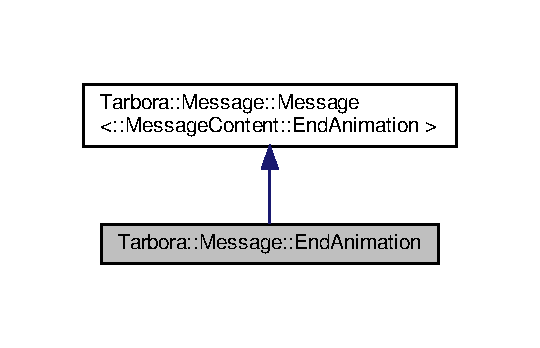
\includegraphics[width=259pt]{classTarbora_1_1Message_1_1EndAnimation__inherit__graph}
\end{center}
\end{figure}


Collaboration diagram for Tarbora\+:\+:Message\+:\+:End\+Animation\+:
\nopagebreak
\begin{figure}[H]
\begin{center}
\leavevmode
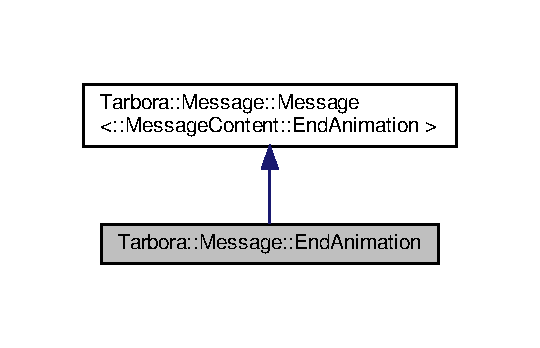
\includegraphics[width=259pt]{classTarbora_1_1Message_1_1EndAnimation__coll__graph}
\end{center}
\end{figure}
\subsection*{Public Member Functions}
\begin{DoxyCompactItemize}
\item 
\mbox{\Hypertarget{classTarbora_1_1Message_1_1EndAnimation_a2ffbb042ca31f55dcc15bd01c540f8a4}\label{classTarbora_1_1Message_1_1EndAnimation_a2ffbb042ca31f55dcc15bd01c540f8a4}} 
{\bfseries End\+Animation} (const \hyperlink{classTarbora_1_1MessageBody}{Message\+Body} \&m)
\item 
\mbox{\Hypertarget{classTarbora_1_1Message_1_1EndAnimation_a4f3cbe8ddbdad7e08a90a03b69b13f50}\label{classTarbora_1_1Message_1_1EndAnimation_a4f3cbe8ddbdad7e08a90a03b69b13f50}} 
{\bfseries End\+Animation} (const Actor\+Id \&id, const std\+::string animation)
\item 
\mbox{\Hypertarget{classTarbora_1_1Message_1_1EndAnimation_a93d25f07aacf24391432931fdabd33a9}\label{classTarbora_1_1Message_1_1EndAnimation_a93d25f07aacf24391432931fdabd33a9}} 
{\bfseries End\+Animation} (const Actor\+Id \&id, const std\+::string animation, int stop\+\_\+mode)
\item 
\mbox{\Hypertarget{classTarbora_1_1Message_1_1EndAnimation_a029d4e1e00cec0517e57346153aaa598}\label{classTarbora_1_1Message_1_1EndAnimation_a029d4e1e00cec0517e57346153aaa598}} 
void {\bfseries set\+Fade\+Out\+Timer} (float timer)
\item 
\mbox{\Hypertarget{classTarbora_1_1Message_1_1EndAnimation_af914e3f0edbfffa24feab22490c6e593}\label{classTarbora_1_1Message_1_1EndAnimation_af914e3f0edbfffa24feab22490c6e593}} 
const Actor\+Id \& {\bfseries get\+Id} ()
\item 
\mbox{\Hypertarget{classTarbora_1_1Message_1_1EndAnimation_a5d43a4c9fc97db59d4e17aab37862ba0}\label{classTarbora_1_1Message_1_1EndAnimation_a5d43a4c9fc97db59d4e17aab37862ba0}} 
const std\+::string \& {\bfseries get\+Animation} ()
\item 
\mbox{\Hypertarget{classTarbora_1_1Message_1_1EndAnimation_a01176b41bbbd479cd724cae3e1d778a7}\label{classTarbora_1_1Message_1_1EndAnimation_a01176b41bbbd479cd724cae3e1d778a7}} 
int {\bfseries get\+Stop\+Mode} ()
\item 
\mbox{\Hypertarget{classTarbora_1_1Message_1_1EndAnimation_a87a9343fc6a89bbd6861274283bfb6b0}\label{classTarbora_1_1Message_1_1EndAnimation_a87a9343fc6a89bbd6861274283bfb6b0}} 
float {\bfseries get\+Fade\+Out\+Timer} ()
\end{DoxyCompactItemize}
\subsection*{Additional Inherited Members}


The documentation for this class was generated from the following file\+:\begin{DoxyCompactItemize}
\item 
Tarbora/\+Messages/Basic\+Messages.\+hpp\end{DoxyCompactItemize}

\hypertarget{classTarbora_1_1GameLayer}{}\section{Tarbora\+:\+:Game\+Layer Class Reference}
\label{classTarbora_1_1GameLayer}\index{Tarbora\+::\+Game\+Layer@{Tarbora\+::\+Game\+Layer}}


Inheritance diagram for Tarbora\+:\+:Game\+Layer\+:\nopagebreak
\begin{figure}[H]
\begin{center}
\leavevmode
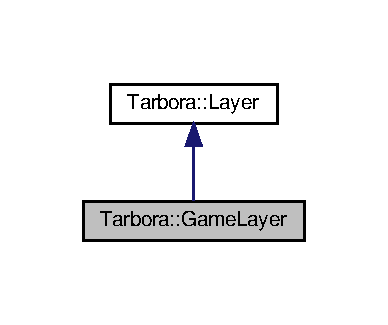
\includegraphics[width=186pt]{classTarbora_1_1GameLayer__inherit__graph}
\end{center}
\end{figure}


Collaboration diagram for Tarbora\+:\+:Game\+Layer\+:\nopagebreak
\begin{figure}[H]
\begin{center}
\leavevmode
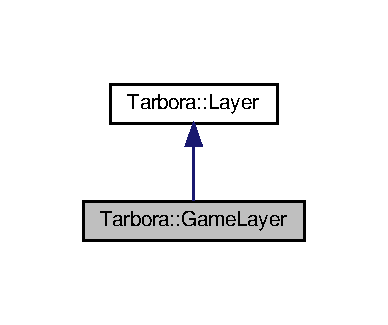
\includegraphics[width=186pt]{classTarbora_1_1GameLayer__coll__graph}
\end{center}
\end{figure}
\subsection*{Public Member Functions}
\begin{DoxyCompactItemize}
\item 
\mbox{\Hypertarget{classTarbora_1_1GameLayer_a3847c040b2c15631e725e8c6ce5ad45b}\label{classTarbora_1_1GameLayer_a3847c040b2c15631e725e8c6ce5ad45b}} 
{\bfseries Game\+Layer} (bool start\+\_\+active=true)
\item 
\mbox{\Hypertarget{classTarbora_1_1GameLayer_a8721890fc92132ba29840cd5a6660cb0}\label{classTarbora_1_1GameLayer_a8721890fc92132ba29840cd5a6660cb0}} 
virtual bool {\bfseries On\+Event} (\hyperlink{structTarbora_1_1Event}{Event} $\ast$e) override
\item 
\mbox{\Hypertarget{classTarbora_1_1GameLayer_a0e9a1674da8efb1c22e38afd38db8712}\label{classTarbora_1_1GameLayer_a0e9a1674da8efb1c22e38afd38db8712}} 
void {\bfseries Update} (float delta\+Time) override
\item 
\mbox{\Hypertarget{classTarbora_1_1GameLayer_a4f511121ff4d7a0b3b93e62c047b3a7e}\label{classTarbora_1_1GameLayer_a4f511121ff4d7a0b3b93e62c047b3a7e}} 
void {\bfseries Draw} () override
\item 
\mbox{\Hypertarget{classTarbora_1_1GameLayer_acc5698563557cb438eb3cc10ef6fef43}\label{classTarbora_1_1GameLayer_acc5698563557cb438eb3cc10ef6fef43}} 
Skybox\+Ptr {\bfseries Get\+Skybox} () const
\item 
\mbox{\Hypertarget{classTarbora_1_1GameLayer_a9a20a0c5d3a1bde8ebb1560771787513}\label{classTarbora_1_1GameLayer_a9a20a0c5d3a1bde8ebb1560771787513}} 
void {\bfseries Set\+Target\+Id} (Actor\+Id id)
\item 
\mbox{\Hypertarget{classTarbora_1_1GameLayer_a18d2cdf99a18fa88bf2c91f8093d9921}\label{classTarbora_1_1GameLayer_a18d2cdf99a18fa88bf2c91f8093d9921}} 
Actor\+Id {\bfseries Get\+Target\+Id} () const
\end{DoxyCompactItemize}


The documentation for this class was generated from the following file\+:\begin{DoxyCompactItemize}
\item 
Tarbora/\+Game\+View/inc/Game\+Layer.\+hpp\end{DoxyCompactItemize}

\hypertarget{classTarbora_1_1GraphicsEngine}{}\section{Tarbora\+:\+:Graphics\+Engine Class Reference}
\label{classTarbora_1_1GraphicsEngine}\index{Tarbora\+::\+Graphics\+Engine@{Tarbora\+::\+Graphics\+Engine}}
\subsection*{Public Member Functions}
\begin{DoxyCompactItemize}
\item 
\mbox{\Hypertarget{classTarbora_1_1GraphicsEngine_a790ece88a0d85e7cffdaa93072701f86}\label{classTarbora_1_1GraphicsEngine_a790ece88a0d85e7cffdaa93072701f86}} 
{\bfseries Graphics\+Engine} (\hyperlink{classTarbora_1_1Module}{Module} $\ast$module, const std\+::string \&settings\+\_\+file)
\item 
\mbox{\Hypertarget{classTarbora_1_1GraphicsEngine_a8a00110a43890767bc2f00f0fe855f9b}\label{classTarbora_1_1GraphicsEngine_a8a00110a43890767bc2f00f0fe855f9b}} 
void {\bfseries before\+Draw} ()
\item 
\mbox{\Hypertarget{classTarbora_1_1GraphicsEngine_a0e929d09863ced274d20980268453869}\label{classTarbora_1_1GraphicsEngine_a0e929d09863ced274d20980268453869}} 
void {\bfseries after\+Draw} ()
\item 
\mbox{\Hypertarget{classTarbora_1_1GraphicsEngine_a8f59fcb64bcb9aba4fec1acec076eb84}\label{classTarbora_1_1GraphicsEngine_a8f59fcb64bcb9aba4fec1acec076eb84}} 
std\+::shared\+\_\+ptr$<$ \hyperlink{classTarbora_1_1Window}{Window} $>$ {\bfseries get\+Window} ()
\item 
\mbox{\Hypertarget{classTarbora_1_1GraphicsEngine_a42a15fe1c1a89ec929b837be6594b5f9}\label{classTarbora_1_1GraphicsEngine_a42a15fe1c1a89ec929b837be6594b5f9}} 
std\+::shared\+\_\+ptr$<$ \hyperlink{classTarbora_1_1RenderQueue}{Render\+Queue} $>$ {\bfseries get\+Render\+Queue} ()
\item 
\mbox{\Hypertarget{classTarbora_1_1GraphicsEngine_ad02c346769f3cef4778f969cf96ab3f4}\label{classTarbora_1_1GraphicsEngine_ad02c346769f3cef4778f969cf96ab3f4}} 
std\+::shared\+\_\+ptr$<$ \hyperlink{classTarbora_1_1Input}{Input} $>$ {\bfseries get\+Input\+Manager} ()
\item 
\mbox{\Hypertarget{classTarbora_1_1GraphicsEngine_af11e3691a81a82743499b9f5b9a6f096}\label{classTarbora_1_1GraphicsEngine_af11e3691a81a82743499b9f5b9a6f096}} 
\hyperlink{classTarbora_1_1Module}{Module} $\ast$ {\bfseries get\+Module} ()
\end{DoxyCompactItemize}


The documentation for this class was generated from the following files\+:\begin{DoxyCompactItemize}
\item 
Tarbora/\+Views/\+Graphic\+Views/\+Graphics\+Engine/Graphics\+Engine.\+hpp\item 
Tarbora/\+Views/\+Graphic\+Views/\+Graphics\+Engine/Graphics\+Engine.\+cpp\end{DoxyCompactItemize}

\hypertarget{classTarbora_1_1GraphicView}{}\section{Tarbora\+:\+:Graphic\+View Class Reference}
\label{classTarbora_1_1GraphicView}\index{Tarbora\+::\+Graphic\+View@{Tarbora\+::\+Graphic\+View}}


Inheritance diagram for Tarbora\+:\+:Graphic\+View\+:\nopagebreak
\begin{figure}[H]
\begin{center}
\leavevmode
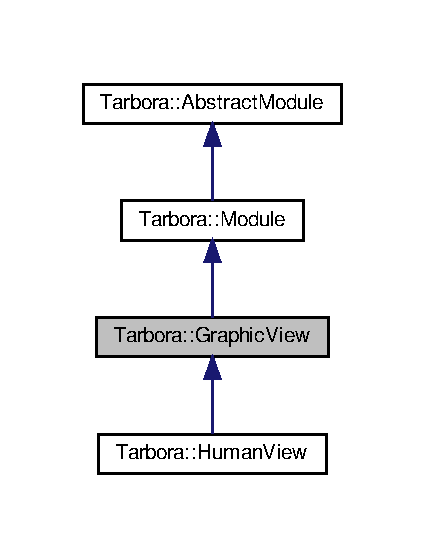
\includegraphics[width=204pt]{classTarbora_1_1GraphicView__inherit__graph}
\end{center}
\end{figure}


Collaboration diagram for Tarbora\+:\+:Graphic\+View\+:\nopagebreak
\begin{figure}[H]
\begin{center}
\leavevmode
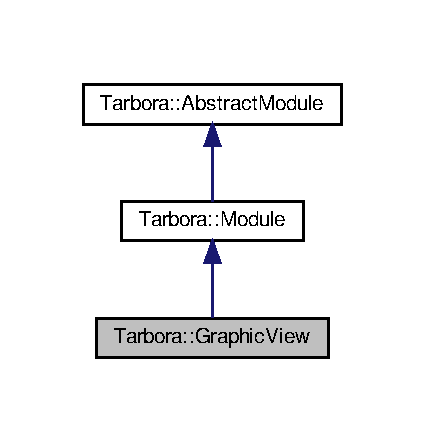
\includegraphics[width=204pt]{classTarbora_1_1GraphicView__coll__graph}
\end{center}
\end{figure}
\subsection*{Public Member Functions}
\begin{DoxyCompactItemize}
\item 
\mbox{\Hypertarget{classTarbora_1_1GraphicView_aae376fc7aaccdad026f7c841f6577fa5}\label{classTarbora_1_1GraphicView_aae376fc7aaccdad026f7c841f6577fa5}} 
{\bfseries Graphic\+View} (const Client\+Id \&client\+\_\+id, const std\+::string \&settings\+\_\+file)
\item 
\mbox{\Hypertarget{classTarbora_1_1GraphicView_ad070d4538da994ad77f8fbfc5bd39763}\label{classTarbora_1_1GraphicView_ad070d4538da994ad77f8fbfc5bd39763}} 
std\+::shared\+\_\+ptr$<$ \hyperlink{classTarbora_1_1GraphicsEngine}{Graphics\+Engine} $>$ {\bfseries get\+Graphics\+Engine} ()
\end{DoxyCompactItemize}
\subsection*{Additional Inherited Members}


The documentation for this class was generated from the following file\+:\begin{DoxyCompactItemize}
\item 
Tarbora/\+Views/\+Graphic\+Views/Graphic\+View.\+hpp\end{DoxyCompactItemize}

\hypertarget{classTarbora_1_1Gui}{}\section{Tarbora\+:\+:Gui Class Reference}
\label{classTarbora_1_1Gui}\index{Tarbora\+::\+Gui@{Tarbora\+::\+Gui}}
\subsection*{Public Member Functions}
\begin{DoxyCompactItemize}
\item 
\mbox{\Hypertarget{classTarbora_1_1Gui_a0a10aa5be9231d8aaef71240b6a8f627}\label{classTarbora_1_1Gui_a0a10aa5be9231d8aaef71240b6a8f627}} 
{\bfseries Gui} (\hyperlink{classTarbora_1_1GraphicView}{Graphic\+View} $\ast$m\+\_\+\+View)
\item 
\mbox{\Hypertarget{classTarbora_1_1Gui_ad54c6113521ed94d15dac59236b75eba}\label{classTarbora_1_1Gui_ad54c6113521ed94d15dac59236b75eba}} 
void {\bfseries Before\+Draw} ()
\item 
\mbox{\Hypertarget{classTarbora_1_1Gui_ada60edc7d56f37a97a966be65c64c74c}\label{classTarbora_1_1Gui_ada60edc7d56f37a97a966be65c64c74c}} 
void {\bfseries After\+Draw} ()
\end{DoxyCompactItemize}


The documentation for this class was generated from the following files\+:\begin{DoxyCompactItemize}
\item 
Tarbora/\+Views/\+Graphics\+Engine/inc/Gui.\+hpp\item 
Tarbora/\+Views/\+Graphics\+Engine/src/Gui.\+cpp\end{DoxyCompactItemize}

\hypertarget{classTarbora_1_1HumanView}{}\section{Tarbora\+:\+:Human\+View Class Reference}
\label{classTarbora_1_1HumanView}\index{Tarbora\+::\+Human\+View@{Tarbora\+::\+Human\+View}}


Inheritance diagram for Tarbora\+:\+:Human\+View\+:\nopagebreak
\begin{figure}[H]
\begin{center}
\leavevmode
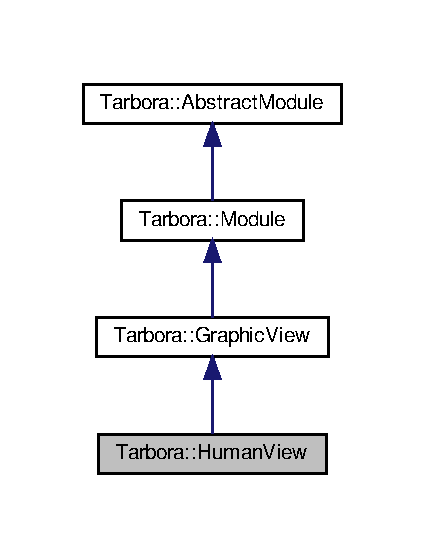
\includegraphics[width=189pt]{classTarbora_1_1HumanView__inherit__graph}
\end{center}
\end{figure}


Collaboration diagram for Tarbora\+:\+:Human\+View\+:\nopagebreak
\begin{figure}[H]
\begin{center}
\leavevmode
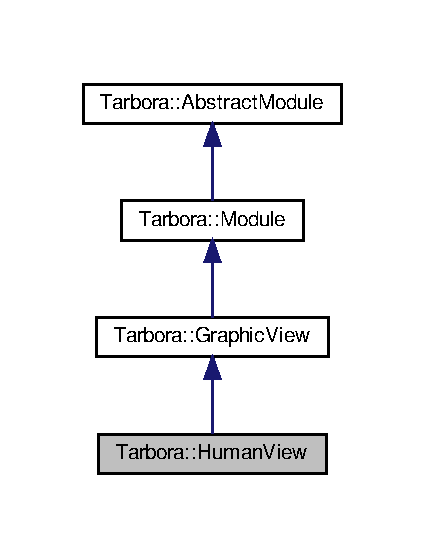
\includegraphics[width=189pt]{classTarbora_1_1HumanView__coll__graph}
\end{center}
\end{figure}
\subsection*{Public Member Functions}
\begin{DoxyCompactItemize}
\item 
\mbox{\Hypertarget{classTarbora_1_1HumanView_aa8cb78e48fc80415f510c1c6f602b9ad}\label{classTarbora_1_1HumanView_aa8cb78e48fc80415f510c1c6f602b9ad}} 
{\bfseries Human\+View} (Actor\+Id id)
\item 
\mbox{\Hypertarget{classTarbora_1_1HumanView_a06d793557524a02d65a6a6b71bfecb14}\label{classTarbora_1_1HumanView_a06d793557524a02d65a6a6b71bfecb14}} 
virtual void {\bfseries Update} (float elapsed\+\_\+time) override
\item 
\mbox{\Hypertarget{classTarbora_1_1HumanView_a0b7e7db0f511c36bac18c51a7e897731}\label{classTarbora_1_1HumanView_a0b7e7db0f511c36bac18c51a7e897731}} 
virtual void {\bfseries Draw} () override
\item 
\mbox{\Hypertarget{classTarbora_1_1HumanView_ab6b2d5d60456394ec63b26f6d7165999}\label{classTarbora_1_1HumanView_ab6b2d5d60456394ec63b26f6d7165999}} 
virtual Actor\+Id {\bfseries Get\+Target\+Id} () const override
\item 
\mbox{\Hypertarget{classTarbora_1_1HumanView_ab28ff0f3d95224b13bb7244183737d1c}\label{classTarbora_1_1HumanView_ab28ff0f3d95224b13bb7244183737d1c}} 
virtual Game\+View\+Type {\bfseries Get\+Type} () const override
\item 
\mbox{\Hypertarget{classTarbora_1_1HumanView_a4e759e449f1d866a693b9397b9c42c42}\label{classTarbora_1_1HumanView_a4e759e449f1d866a693b9397b9c42c42}} 
virtual void {\bfseries Push\+Layer} (std\+::shared\+\_\+ptr$<$ \hyperlink{classTarbora_1_1Layer}{Layer} $>$ layer)
\item 
\mbox{\Hypertarget{classTarbora_1_1HumanView_a766f8e93c1e7477f87f300e833deb08d}\label{classTarbora_1_1HumanView_a766f8e93c1e7477f87f300e833deb08d}} 
virtual void {\bfseries Remove\+Layer} (std\+::shared\+\_\+ptr$<$ \hyperlink{classTarbora_1_1Layer}{Layer} $>$ layer)
\end{DoxyCompactItemize}
\subsection*{Protected Attributes}
\begin{DoxyCompactItemize}
\item 
\mbox{\Hypertarget{classTarbora_1_1HumanView_a3f61b24596499e6249136efd22a2b818}\label{classTarbora_1_1HumanView_a3f61b24596499e6249136efd22a2b818}} 
std\+::shared\+\_\+ptr$<$ \hyperlink{classTarbora_1_1GameLayer}{Game\+Layer} $>$ {\bfseries m\+\_\+\+Game\+Layer}
\item 
\mbox{\Hypertarget{classTarbora_1_1HumanView_a09f3664c6d9e79bc83054fd3df4bfa2e}\label{classTarbora_1_1HumanView_a09f3664c6d9e79bc83054fd3df4bfa2e}} 
Layer\+List {\bfseries m\+\_\+\+Layers}
\item 
\mbox{\Hypertarget{classTarbora_1_1HumanView_a1f31d17eebef84fd84ef6ff1d38b1c12}\label{classTarbora_1_1HumanView_a1f31d17eebef84fd84ef6ff1d38b1c12}} 
unsigned int {\bfseries Evt\+Key\+Press\+Id}
\item 
\mbox{\Hypertarget{classTarbora_1_1HumanView_ad2ddebb6ba7685ea70fc5982bd81c04a}\label{classTarbora_1_1HumanView_ad2ddebb6ba7685ea70fc5982bd81c04a}} 
unsigned int {\bfseries Evt\+Key\+Release\+Id}
\item 
\mbox{\Hypertarget{classTarbora_1_1HumanView_a428fde63f13aa68167d54afea96e77fe}\label{classTarbora_1_1HumanView_a428fde63f13aa68167d54afea96e77fe}} 
unsigned int {\bfseries Evt\+Button\+Press\+Id}
\item 
\mbox{\Hypertarget{classTarbora_1_1HumanView_a0277cc15f329ce840c431ee079ec06be}\label{classTarbora_1_1HumanView_a0277cc15f329ce840c431ee079ec06be}} 
unsigned int {\bfseries Evt\+Button\+Release\+Id}
\item 
\mbox{\Hypertarget{classTarbora_1_1HumanView_ae0c4f8670e4a27c1699b94a281b58bbf}\label{classTarbora_1_1HumanView_ae0c4f8670e4a27c1699b94a281b58bbf}} 
unsigned int {\bfseries Evt\+Mouse\+Move\+Id}
\item 
\mbox{\Hypertarget{classTarbora_1_1HumanView_aa870c7ef3d3bccaba17d160c45eadbdc}\label{classTarbora_1_1HumanView_aa870c7ef3d3bccaba17d160c45eadbdc}} 
unsigned int {\bfseries Evt\+Mouse\+Scroll\+Id}
\end{DoxyCompactItemize}


The documentation for this class was generated from the following files\+:\begin{DoxyCompactItemize}
\item 
Tarbora/\+Game\+View/inc/Human\+View.\+hpp\item 
Tarbora/\+Game\+View/src/Human\+View.\+cpp\end{DoxyCompactItemize}

\hypertarget{classTarbora_1_1InfoComponent}{}\section{Tarbora\+:\+:Info\+Component Class Reference}
\label{classTarbora_1_1InfoComponent}\index{Tarbora\+::\+Info\+Component@{Tarbora\+::\+Info\+Component}}


Inheritance diagram for Tarbora\+:\+:Info\+Component\+:\nopagebreak
\begin{figure}[H]
\begin{center}
\leavevmode
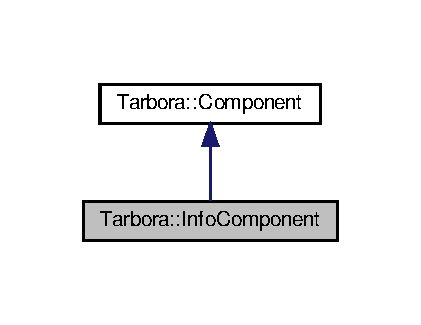
\includegraphics[width=202pt]{classTarbora_1_1InfoComponent__inherit__graph}
\end{center}
\end{figure}


Collaboration diagram for Tarbora\+:\+:Info\+Component\+:\nopagebreak
\begin{figure}[H]
\begin{center}
\leavevmode
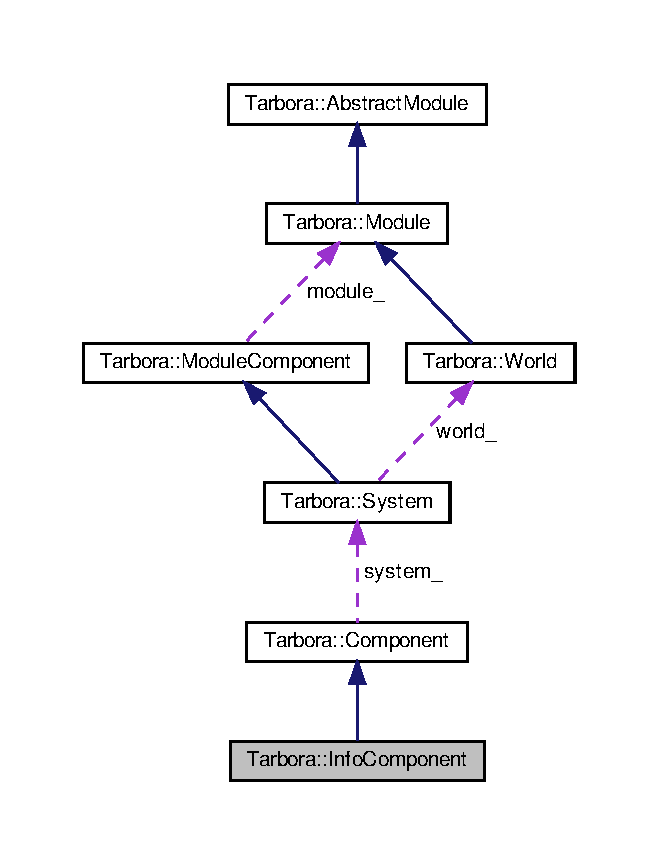
\includegraphics[width=316pt]{classTarbora_1_1InfoComponent__coll__graph}
\end{center}
\end{figure}
\subsection*{Public Member Functions}
\begin{DoxyCompactItemize}
\item 
\mbox{\Hypertarget{classTarbora_1_1InfoComponent_a02d7b59bac3005f9d64bf23ca9b355e6}\label{classTarbora_1_1InfoComponent_a02d7b59bac3005f9d64bf23ca9b355e6}} 
{\bfseries Info\+Component} (\hyperlink{classTarbora_1_1System}{System} $\ast$s, const Actor\+Id \&id, const \hyperlink{classTarbora_1_1LuaTable}{Lua\+Table} \&table)
\item 
\mbox{\Hypertarget{classTarbora_1_1InfoComponent_ac97874d9cab2a24cfc92a7d847614bd0}\label{classTarbora_1_1InfoComponent_ac97874d9cab2a24cfc92a7d847614bd0}} 
const std\+::string \& {\bfseries get\+Entity} ()
\item 
\mbox{\Hypertarget{classTarbora_1_1InfoComponent_a1aaab6d0d64bd6b5712a6ab887e4dc37}\label{classTarbora_1_1InfoComponent_a1aaab6d0d64bd6b5712a6ab887e4dc37}} 
const std\+::string \& {\bfseries get\+Variant} ()
\end{DoxyCompactItemize}
\subsection*{Additional Inherited Members}


The documentation for this class was generated from the following file\+:\begin{DoxyCompactItemize}
\item 
Tarbora/\+Logic/Info\+Component.\+hpp\end{DoxyCompactItemize}

\hypertarget{classTarbora_1_1InfoSystem}{}\section{Tarbora\+:\+:Info\+System Class Reference}
\label{classTarbora_1_1InfoSystem}\index{Tarbora\+::\+Info\+System@{Tarbora\+::\+Info\+System}}


Inheritance diagram for Tarbora\+:\+:Info\+System\+:\nopagebreak
\begin{figure}[H]
\begin{center}
\leavevmode
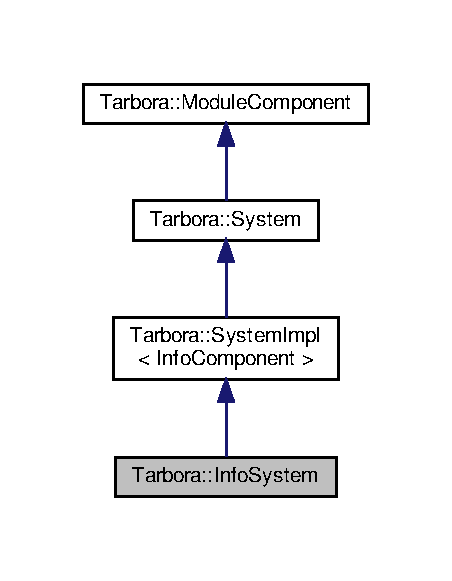
\includegraphics[width=217pt]{classTarbora_1_1InfoSystem__inherit__graph}
\end{center}
\end{figure}


Collaboration diagram for Tarbora\+:\+:Info\+System\+:\nopagebreak
\begin{figure}[H]
\begin{center}
\leavevmode
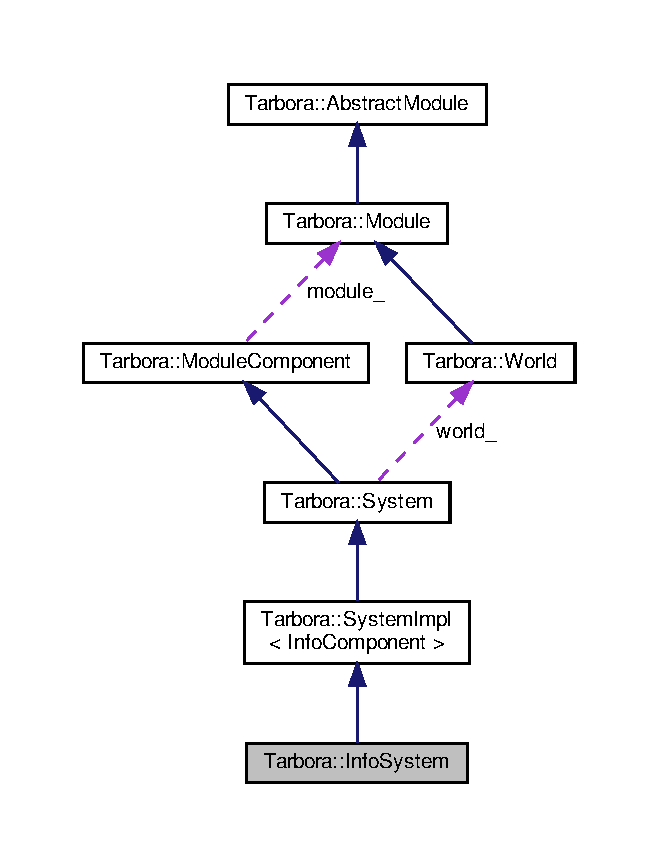
\includegraphics[width=316pt]{classTarbora_1_1InfoSystem__coll__graph}
\end{center}
\end{figure}
\subsection*{Public Member Functions}
\begin{DoxyCompactItemize}
\item 
\mbox{\Hypertarget{classTarbora_1_1InfoSystem_aa51ed7d2c8080dcaec3ab3f885bb20da}\label{classTarbora_1_1InfoSystem_aa51ed7d2c8080dcaec3ab3f885bb20da}} 
{\bfseries Info\+System} (\hyperlink{classTarbora_1_1World}{World} $\ast$w)
\end{DoxyCompactItemize}
\subsection*{Static Public Member Functions}
\begin{DoxyCompactItemize}
\item 
\mbox{\Hypertarget{classTarbora_1_1InfoSystem_a12d888ad9d36d89e2d54b25540a6dbae}\label{classTarbora_1_1InfoSystem_a12d888ad9d36d89e2d54b25540a6dbae}} 
static std\+::string {\bfseries get\+Name} ()
\end{DoxyCompactItemize}
\subsection*{Additional Inherited Members}


The documentation for this class was generated from the following file\+:\begin{DoxyCompactItemize}
\item 
Tarbora/\+Logic/Info\+Component.\+hpp\end{DoxyCompactItemize}

\hypertarget{classTarbora_1_1Input}{}\section{Tarbora\+:\+:Input Class Reference}
\label{classTarbora_1_1Input}\index{Tarbora\+::\+Input@{Tarbora\+::\+Input}}
\subsection*{Public Types}
\begin{DoxyCompactItemize}
\item 
\mbox{\Hypertarget{classTarbora_1_1Input_ada5f47dd8b178a810ba4f50f3797fe4a}\label{classTarbora_1_1Input_ada5f47dd8b178a810ba4f50f3797fe4a}} 
enum {\bfseries State} \{ {\bfseries U\+N\+C\+H\+A\+N\+G\+ED}, 
{\bfseries UP}, 
{\bfseries D\+O\+WN}
 \}
\end{DoxyCompactItemize}
\subsection*{Public Member Functions}
\begin{DoxyCompactItemize}
\item 
\mbox{\Hypertarget{classTarbora_1_1Input_a55a9e2f2a9975190ba1a4988a160b565}\label{classTarbora_1_1Input_a55a9e2f2a9975190ba1a4988a160b565}} 
{\bfseries Input} (\hyperlink{classTarbora_1_1GraphicsEngine}{Graphics\+Engine} $\ast$graphics\+Engine)
\item 
\mbox{\Hypertarget{classTarbora_1_1Input_ac6a1c81cb6cd595c416249d4487a8435}\label{classTarbora_1_1Input_ac6a1c81cb6cd595c416249d4487a8435}} 
bool {\bfseries get\+Key} (int keycode)
\item 
\mbox{\Hypertarget{classTarbora_1_1Input_a69f64f63c65110a9ee1ba2c3cda9a51b}\label{classTarbora_1_1Input_a69f64f63c65110a9ee1ba2c3cda9a51b}} 
bool {\bfseries get\+Key\+Down} (int keycode)
\item 
\mbox{\Hypertarget{classTarbora_1_1Input_a5cb01354fffe3ffde262870965e4f1ab}\label{classTarbora_1_1Input_a5cb01354fffe3ffde262870965e4f1ab}} 
bool {\bfseries get\+Key\+Up} (int keycode)
\item 
\mbox{\Hypertarget{classTarbora_1_1Input_a1f563b437cf29d3d690fae48a5f58d2f}\label{classTarbora_1_1Input_a1f563b437cf29d3d690fae48a5f58d2f}} 
State {\bfseries get\+Key\+State} (int keycode)
\item 
\mbox{\Hypertarget{classTarbora_1_1Input_a01201a11a22db928da24da9aea7c2c43}\label{classTarbora_1_1Input_a01201a11a22db928da24da9aea7c2c43}} 
void {\bfseries set\+Key\+State} (int keycode, State state)
\item 
\mbox{\Hypertarget{classTarbora_1_1Input_af000902d489f55f74d3fd207cbb6098a}\label{classTarbora_1_1Input_af000902d489f55f74d3fd207cbb6098a}} 
bool {\bfseries get\+Button} (int button)
\item 
\mbox{\Hypertarget{classTarbora_1_1Input_a98a069825636b97e00e78cfb56023b3e}\label{classTarbora_1_1Input_a98a069825636b97e00e78cfb56023b3e}} 
bool {\bfseries get\+Button\+Down} (int button)
\item 
\mbox{\Hypertarget{classTarbora_1_1Input_a46ec433c57de113534709f0da77b75a8}\label{classTarbora_1_1Input_a46ec433c57de113534709f0da77b75a8}} 
bool {\bfseries get\+Button\+Up} (int button)
\item 
\mbox{\Hypertarget{classTarbora_1_1Input_a19310257065fe20b019474ae783ed8e5}\label{classTarbora_1_1Input_a19310257065fe20b019474ae783ed8e5}} 
State {\bfseries get\+Button\+State} (int button)
\item 
\mbox{\Hypertarget{classTarbora_1_1Input_a22c4a063b5598a1612148ad1fd1f42dc}\label{classTarbora_1_1Input_a22c4a063b5598a1612148ad1fd1f42dc}} 
void {\bfseries set\+Button\+State} (int button, State state)
\item 
\mbox{\Hypertarget{classTarbora_1_1Input_ad102366d6acc777674c6b999bf473d26}\label{classTarbora_1_1Input_ad102366d6acc777674c6b999bf473d26}} 
glm\+::vec2 {\bfseries get\+Mouse\+Position} ()
\item 
\mbox{\Hypertarget{classTarbora_1_1Input_a7088612cd145e5e6ca7532756ef3e277}\label{classTarbora_1_1Input_a7088612cd145e5e6ca7532756ef3e277}} 
glm\+::vec2 {\bfseries get\+Mouse\+Delta} ()
\end{DoxyCompactItemize}


The documentation for this class was generated from the following files\+:\begin{DoxyCompactItemize}
\item 
Tarbora/\+Views/\+Graphic\+Views/\+Graphics\+Engine/Input.\+hpp\item 
Tarbora/\+Views/\+Graphic\+Views/\+Graphics\+Engine/Input.\+cpp\end{DoxyCompactItemize}

\hypertarget{classTarbora_1_1Layer}{}\section{Tarbora\+:\+:Layer Class Reference}
\label{classTarbora_1_1Layer}\index{Tarbora\+::\+Layer@{Tarbora\+::\+Layer}}


Inheritance diagram for Tarbora\+:\+:Layer\+:\nopagebreak
\begin{figure}[H]
\begin{center}
\leavevmode
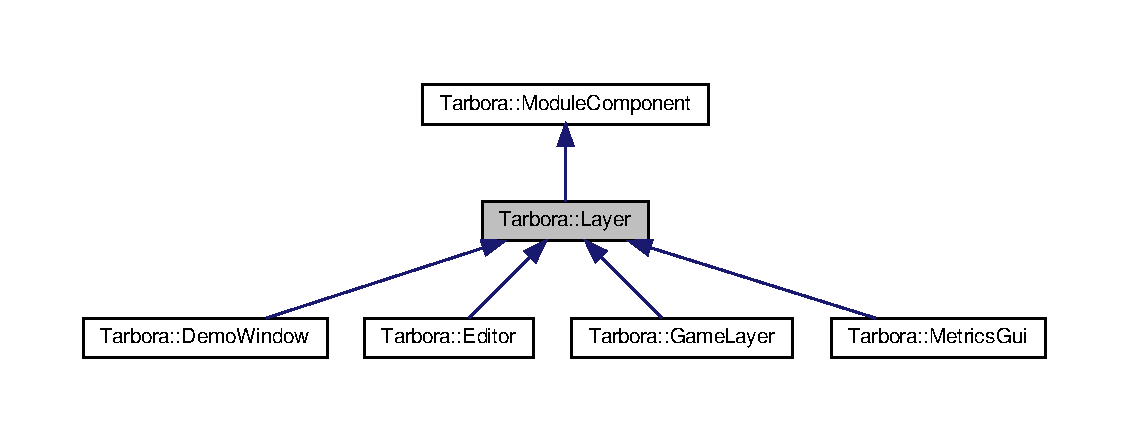
\includegraphics[width=350pt]{classTarbora_1_1Layer__inherit__graph}
\end{center}
\end{figure}


Collaboration diagram for Tarbora\+:\+:Layer\+:\nopagebreak
\begin{figure}[H]
\begin{center}
\leavevmode
\includegraphics[width=217pt]{classTarbora_1_1Layer__coll__graph}
\end{center}
\end{figure}
\subsection*{Public Member Functions}
\begin{DoxyCompactItemize}
\item 
\mbox{\Hypertarget{classTarbora_1_1Layer_a58106508db0aafaec0d5e9bbcf79e24f}\label{classTarbora_1_1Layer_a58106508db0aafaec0d5e9bbcf79e24f}} 
{\bfseries Layer} (\hyperlink{classTarbora_1_1GraphicView}{Graphic\+View} $\ast$view, bool start\+\_\+active=true)
\item 
\mbox{\Hypertarget{classTarbora_1_1Layer_aab6d82e0e2048dc50be2dc3d545c0e7f}\label{classTarbora_1_1Layer_aab6d82e0e2048dc50be2dc3d545c0e7f}} 
virtual void {\bfseries on\+Activate} ()
\item 
\mbox{\Hypertarget{classTarbora_1_1Layer_aaa4c828f3c6fb7ff42e5667805f650c0}\label{classTarbora_1_1Layer_aaa4c828f3c6fb7ff42e5667805f650c0}} 
virtual void {\bfseries on\+Deactivate} ()
\item 
\mbox{\Hypertarget{classTarbora_1_1Layer_a6f06c6331635d6f29b6b711fecafc617}\label{classTarbora_1_1Layer_a6f06c6331635d6f29b6b711fecafc617}} 
virtual void {\bfseries get\+Input} ()
\item 
\mbox{\Hypertarget{classTarbora_1_1Layer_aa840eefc7b9a7fc08f6ca7ba14e219de}\label{classTarbora_1_1Layer_aa840eefc7b9a7fc08f6ca7ba14e219de}} 
virtual void {\bfseries update} (float delta\+\_\+time)
\item 
\mbox{\Hypertarget{classTarbora_1_1Layer_a0744dccca287ad0100f688eba65c9d3f}\label{classTarbora_1_1Layer_a0744dccca287ad0100f688eba65c9d3f}} 
virtual void {\bfseries draw} ()
\item 
\mbox{\Hypertarget{classTarbora_1_1Layer_a246f85b37366ddf34b446331fe7a3447}\label{classTarbora_1_1Layer_a246f85b37366ddf34b446331fe7a3447}} 
virtual bool {\bfseries on\+Message} (const \hyperlink{classTarbora_1_1MessageBody}{Message\+Body} \&m)
\item 
\mbox{\Hypertarget{classTarbora_1_1Layer_a4fc2a9f5064bbd6776bd1ae8398aa734}\label{classTarbora_1_1Layer_a4fc2a9f5064bbd6776bd1ae8398aa734}} 
void {\bfseries set\+Active} (bool active)
\item 
\mbox{\Hypertarget{classTarbora_1_1Layer_a606bb2b75b38acf75e5f4caabceedb97}\label{classTarbora_1_1Layer_a606bb2b75b38acf75e5f4caabceedb97}} 
bool {\bfseries is\+Active} () const
\item 
\mbox{\Hypertarget{classTarbora_1_1Layer_a6f787d1153bdbaf8066e2745d2faf86a}\label{classTarbora_1_1Layer_a6f787d1153bdbaf8066e2745d2faf86a}} 
std\+::shared\+\_\+ptr$<$ \hyperlink{classTarbora_1_1Input}{Input} $>$ {\bfseries get\+Input\+Manager} ()
\end{DoxyCompactItemize}
\subsection*{Protected Attributes}
\begin{DoxyCompactItemize}
\item 
\mbox{\Hypertarget{classTarbora_1_1Layer_a4d7fdc234d3b929bff31b80013355ddb}\label{classTarbora_1_1Layer_a4d7fdc234d3b929bff31b80013355ddb}} 
bool {\bfseries active\+\_\+}
\item 
\mbox{\Hypertarget{classTarbora_1_1Layer_a0c24802fe48c762c865fea4fa6357e04}\label{classTarbora_1_1Layer_a0c24802fe48c762c865fea4fa6357e04}} 
bool {\bfseries event\+\_\+blocking\+\_\+}
\end{DoxyCompactItemize}
\subsection*{Additional Inherited Members}


The documentation for this class was generated from the following file\+:\begin{DoxyCompactItemize}
\item 
Tarbora/\+Views/\+Graphic\+Views/Layer.\+hpp\end{DoxyCompactItemize}

\hypertarget{classTarbora_1_1Logger}{}\section{Tarbora\+:\+:Logger Class Reference}
\label{classTarbora_1_1Logger}\index{Tarbora\+::\+Logger@{Tarbora\+::\+Logger}}
\subsection*{Public Types}
\begin{DoxyCompactItemize}
\item 
\mbox{\Hypertarget{classTarbora_1_1Logger_a0596faea258f2da51ad7ca3abd806be3}\label{classTarbora_1_1Logger_a0596faea258f2da51ad7ca3abd806be3}} 
enum {\bfseries Log\+Level} \{ {\bfseries D\+E\+B\+UG} =0, 
{\bfseries I\+N\+FO}, 
{\bfseries W\+A\+RN}, 
{\bfseries E\+RR}
 \}
\end{DoxyCompactItemize}
\subsection*{Static Public Member Functions}
\begin{DoxyCompactItemize}
\item 
static bool \hyperlink{classTarbora_1_1Logger_abb526de5b2ecd2bda6ec4883de07bec8}{Init} (F\+I\+LE $\ast$stream)
\begin{DoxyCompactList}\small\item\em Initialize the logger to an open stream. \end{DoxyCompactList}\item 
static bool \hyperlink{classTarbora_1_1Logger_a625b88289ed91c3059320a9573e16103}{Init} (std\+::string file\+\_\+path)
\begin{DoxyCompactList}\small\item\em Initialize the logger to a file. \end{DoxyCompactList}\item 
\mbox{\Hypertarget{classTarbora_1_1Logger_add4c310a2ab7b0daa730e477853d6c8f}\label{classTarbora_1_1Logger_add4c310a2ab7b0daa730e477853d6c8f}} 
static void \hyperlink{classTarbora_1_1Logger_add4c310a2ab7b0daa730e477853d6c8f}{Close} ()
\begin{DoxyCompactList}\small\item\em Close the logger. \end{DoxyCompactList}\item 
static void \hyperlink{classTarbora_1_1Logger_af2a11244236bad59fce9cc6a1360af29}{Set\+Level} (Log\+Level level)
\begin{DoxyCompactList}\small\item\em Set the log level. \end{DoxyCompactList}\item 
static void \hyperlink{classTarbora_1_1Logger_aa32641fca455178d88f3b1c8b2f552ab}{Log} (Log\+Level level, const char $\ast$text,...)
\begin{DoxyCompactList}\small\item\em Log a message. \end{DoxyCompactList}\end{DoxyCompactItemize}


\subsection{Member Function Documentation}
\mbox{\Hypertarget{classTarbora_1_1Logger_abb526de5b2ecd2bda6ec4883de07bec8}\label{classTarbora_1_1Logger_abb526de5b2ecd2bda6ec4883de07bec8}} 
\index{Tarbora\+::\+Logger@{Tarbora\+::\+Logger}!Init@{Init}}
\index{Init@{Init}!Tarbora\+::\+Logger@{Tarbora\+::\+Logger}}
\subsubsection{\texorpdfstring{Init()}{Init()}\hspace{0.1cm}{\footnotesize\ttfamily [1/2]}}
{\footnotesize\ttfamily bool Tarbora\+::\+Logger\+::\+Init (\begin{DoxyParamCaption}\item[{F\+I\+LE $\ast$}]{stream }\end{DoxyParamCaption})\hspace{0.3cm}{\ttfamily [static]}}



Initialize the logger to an open stream. 


\begin{DoxyParams}{Parameters}
{\em stream} & The stream (file or console) where the logger will print. \\
\hline
\end{DoxyParams}
\mbox{\Hypertarget{classTarbora_1_1Logger_a625b88289ed91c3059320a9573e16103}\label{classTarbora_1_1Logger_a625b88289ed91c3059320a9573e16103}} 
\index{Tarbora\+::\+Logger@{Tarbora\+::\+Logger}!Init@{Init}}
\index{Init@{Init}!Tarbora\+::\+Logger@{Tarbora\+::\+Logger}}
\subsubsection{\texorpdfstring{Init()}{Init()}\hspace{0.1cm}{\footnotesize\ttfamily [2/2]}}
{\footnotesize\ttfamily bool Tarbora\+::\+Logger\+::\+Init (\begin{DoxyParamCaption}\item[{std\+::string}]{file\+\_\+path }\end{DoxyParamCaption})\hspace{0.3cm}{\ttfamily [static]}}



Initialize the logger to a file. 


\begin{DoxyParams}{Parameters}
{\em file\+\_\+path} & The name of the file where the logger will print. \\
\hline
\end{DoxyParams}
\mbox{\Hypertarget{classTarbora_1_1Logger_aa32641fca455178d88f3b1c8b2f552ab}\label{classTarbora_1_1Logger_aa32641fca455178d88f3b1c8b2f552ab}} 
\index{Tarbora\+::\+Logger@{Tarbora\+::\+Logger}!Log@{Log}}
\index{Log@{Log}!Tarbora\+::\+Logger@{Tarbora\+::\+Logger}}
\subsubsection{\texorpdfstring{Log()}{Log()}}
{\footnotesize\ttfamily void Tarbora\+::\+Logger\+::\+Log (\begin{DoxyParamCaption}\item[{Log\+Level}]{level,  }\item[{const char $\ast$}]{text,  }\item[{}]{... }\end{DoxyParamCaption})\hspace{0.3cm}{\ttfamily [static]}}



Log a message. 


\begin{DoxyParams}{Parameters}
{\em level} & The log level of the message. \\
\hline
{\em text} & The message itself, formatted as a printf. \\
\hline
{\em ...} & The extra params of the printf.\\
\hline
\end{DoxyParams}
It can be called through the macros\+: 
\begin{DoxyCode}
LOG\_DEBUG(TEXT, ...)
LOG\_INFO(TEXT, ...)
LOG\_WARN(TEXT, ...)
LOG\_ERR(TEXT, ...)
\end{DoxyCode}
 \mbox{\Hypertarget{classTarbora_1_1Logger_af2a11244236bad59fce9cc6a1360af29}\label{classTarbora_1_1Logger_af2a11244236bad59fce9cc6a1360af29}} 
\index{Tarbora\+::\+Logger@{Tarbora\+::\+Logger}!Set\+Level@{Set\+Level}}
\index{Set\+Level@{Set\+Level}!Tarbora\+::\+Logger@{Tarbora\+::\+Logger}}
\subsubsection{\texorpdfstring{Set\+Level()}{SetLevel()}}
{\footnotesize\ttfamily void Tarbora\+::\+Logger\+::\+Set\+Level (\begin{DoxyParamCaption}\item[{Log\+Level}]{level }\end{DoxyParamCaption})\hspace{0.3cm}{\ttfamily [static]}}



Set the log level. 


\begin{DoxyParams}{Parameters}
{\em level} & Levels lower than that will be ignored.\\
\hline
\end{DoxyParams}
It can be called through a macro\+: 
\begin{DoxyCode}
LOG\_LEVEL(LEVEL)
\end{DoxyCode}
 

The documentation for this class was generated from the following files\+:\begin{DoxyCompactItemize}
\item 
Tarbora/\+Framework/\+Utility/inc/Logger.\+hpp\item 
Tarbora/\+Framework/\+Utility/src/Logger.\+cpp\end{DoxyCompactItemize}

\hypertarget{classTarbora_1_1Message_1_1LookAt}{}\section{Tarbora\+:\+:Message\+:\+:Look\+At Class Reference}
\label{classTarbora_1_1Message_1_1LookAt}\index{Tarbora\+::\+Message\+::\+Look\+At@{Tarbora\+::\+Message\+::\+Look\+At}}


Inheritance diagram for Tarbora\+:\+:Message\+:\+:Look\+At\+:\nopagebreak
\begin{figure}[H]
\begin{center}
\leavevmode
\includegraphics[width=229pt]{classTarbora_1_1Message_1_1LookAt__inherit__graph}
\end{center}
\end{figure}


Collaboration diagram for Tarbora\+:\+:Message\+:\+:Look\+At\+:\nopagebreak
\begin{figure}[H]
\begin{center}
\leavevmode
\includegraphics[width=229pt]{classTarbora_1_1Message_1_1LookAt__coll__graph}
\end{center}
\end{figure}
\subsection*{Public Member Functions}
\begin{DoxyCompactItemize}
\item 
\mbox{\Hypertarget{classTarbora_1_1Message_1_1LookAt_a3d775594bc15f9ea91ed3e460f2f0c1e}\label{classTarbora_1_1Message_1_1LookAt_a3d775594bc15f9ea91ed3e460f2f0c1e}} 
{\bfseries Look\+At} (const \hyperlink{classTarbora_1_1MessageBody}{Message\+Body} \&m)
\item 
\mbox{\Hypertarget{classTarbora_1_1Message_1_1LookAt_a489b1d86d421f5fc041891452dbc5b05}\label{classTarbora_1_1Message_1_1LookAt_a489b1d86d421f5fc041891452dbc5b05}} 
{\bfseries Look\+At} (const Actor\+Id \&id, const glm\+::vec3 \&direction)
\item 
\mbox{\Hypertarget{classTarbora_1_1Message_1_1LookAt_a317eee28d4aae9c94e1a8a524d17d8f2}\label{classTarbora_1_1Message_1_1LookAt_a317eee28d4aae9c94e1a8a524d17d8f2}} 
{\bfseries Look\+At} (const Actor\+Id \&id, const Actor\+Id \&target)
\item 
\mbox{\Hypertarget{classTarbora_1_1Message_1_1LookAt_a27d66789fb1ef6fdb120c06ac6224f55}\label{classTarbora_1_1Message_1_1LookAt_a27d66789fb1ef6fdb120c06ac6224f55}} 
{\bfseries Look\+At} (const Actor\+Id \&id, const Actor\+Id \&target, float distance)
\item 
\mbox{\Hypertarget{classTarbora_1_1Message_1_1LookAt_a1fd337a8fd3b3e28148b8e4c2a45e6d7}\label{classTarbora_1_1Message_1_1LookAt_a1fd337a8fd3b3e28148b8e4c2a45e6d7}} 
const Actor\+Id \& {\bfseries get\+Id} ()
\item 
\mbox{\Hypertarget{classTarbora_1_1Message_1_1LookAt_a4b591d43b26663009acf4c3df1f71512}\label{classTarbora_1_1Message_1_1LookAt_a4b591d43b26663009acf4c3df1f71512}} 
const Actor\+Id \& {\bfseries get\+Target} ()
\item 
\mbox{\Hypertarget{classTarbora_1_1Message_1_1LookAt_ae60b2a2635757c25fe6c9131aba223ce}\label{classTarbora_1_1Message_1_1LookAt_ae60b2a2635757c25fe6c9131aba223ce}} 
float {\bfseries get\+Distance} ()
\item 
\mbox{\Hypertarget{classTarbora_1_1Message_1_1LookAt_a8bbb04658266cd4219d81280997de332}\label{classTarbora_1_1Message_1_1LookAt_a8bbb04658266cd4219d81280997de332}} 
glm\+::vec3 {\bfseries get\+Direction} ()
\item 
\mbox{\Hypertarget{classTarbora_1_1Message_1_1LookAt_ad7bf541789ffe467b18cd403d74a4bb4}\label{classTarbora_1_1Message_1_1LookAt_ad7bf541789ffe467b18cd403d74a4bb4}} 
bool {\bfseries has\+Direction} ()
\end{DoxyCompactItemize}
\subsection*{Additional Inherited Members}


The documentation for this class was generated from the following file\+:\begin{DoxyCompactItemize}
\item 
Tarbora/\+Messages/Basic\+Messages.\+hpp\end{DoxyCompactItemize}

\hypertarget{classTarbora_1_1LuaFunction}{}\section{Tarbora\+:\+:Lua\+Function$<$ T $>$ Class Template Reference}
\label{classTarbora_1_1LuaFunction}\index{Tarbora\+::\+Lua\+Function$<$ T $>$@{Tarbora\+::\+Lua\+Function$<$ T $>$}}
\subsection*{Public Member Functions}
\begin{DoxyCompactItemize}
\item 
\mbox{\Hypertarget{classTarbora_1_1LuaFunction_a2d570c5008fff45a2c6b3219690959a3}\label{classTarbora_1_1LuaFunction_a2d570c5008fff45a2c6b3219690959a3}} 
{\bfseries Lua\+Function} (sol\+::state $\ast$state, const sol\+::protected\+\_\+function \&function, const std\+::string \&name, bool silent)
\item 
\mbox{\Hypertarget{classTarbora_1_1LuaFunction_a7915f7c679987d5f5645cb259ff6cc60}\label{classTarbora_1_1LuaFunction_a7915f7c679987d5f5645cb259ff6cc60}} 
bool {\bfseries valid} () const
\item 
\mbox{\Hypertarget{classTarbora_1_1LuaFunction_af2d444cf8d3d32bec3ed038c90901c9a}\label{classTarbora_1_1LuaFunction_af2d444cf8d3d32bec3ed038c90901c9a}} 
{\footnotesize template$<$class... Args$>$ }\\T {\bfseries operator()} (Args \&\&... args)
\item 
\mbox{\Hypertarget{classTarbora_1_1LuaFunction_ab32291caf4a74910113389ff6c6e5aab}\label{classTarbora_1_1LuaFunction_ab32291caf4a74910113389ff6c6e5aab}} 
{\footnotesize template$<$$>$ }\\void {\bfseries operator()} (Args \&\&... args)
\end{DoxyCompactItemize}


The documentation for this class was generated from the following file\+:\begin{DoxyCompactItemize}
\item 
Tarbora/\+Framework/\+Resource\+Manager/Lua.\+hpp\end{DoxyCompactItemize}

\hypertarget{classTarbora_1_1LuaFunction_3_01std_1_1vector_3_01T_01_4_01_4}{}\section{Tarbora\+:\+:Lua\+Function$<$ std\+:\+:vector$<$ T $>$ $>$ Class Template Reference}
\label{classTarbora_1_1LuaFunction_3_01std_1_1vector_3_01T_01_4_01_4}\index{Tarbora\+::\+Lua\+Function$<$ std\+::vector$<$ T $>$ $>$@{Tarbora\+::\+Lua\+Function$<$ std\+::vector$<$ T $>$ $>$}}
\subsection*{Public Member Functions}
\begin{DoxyCompactItemize}
\item 
\mbox{\Hypertarget{classTarbora_1_1LuaFunction_3_01std_1_1vector_3_01T_01_4_01_4_ab83581d0db66993d733ba6df2f0b550a}\label{classTarbora_1_1LuaFunction_3_01std_1_1vector_3_01T_01_4_01_4_ab83581d0db66993d733ba6df2f0b550a}} 
{\bfseries Lua\+Function} (sol\+::state $\ast$state, const sol\+::protected\+\_\+function \&function, const std\+::string \&name, bool silent)
\item 
\mbox{\Hypertarget{classTarbora_1_1LuaFunction_3_01std_1_1vector_3_01T_01_4_01_4_aa0bb340fcd4e0598acfd1f98a534cb96}\label{classTarbora_1_1LuaFunction_3_01std_1_1vector_3_01T_01_4_01_4_aa0bb340fcd4e0598acfd1f98a534cb96}} 
bool {\bfseries valid} () const
\item 
\mbox{\Hypertarget{classTarbora_1_1LuaFunction_3_01std_1_1vector_3_01T_01_4_01_4_a200134fef7b06174b2c1cd3037292686}\label{classTarbora_1_1LuaFunction_3_01std_1_1vector_3_01T_01_4_01_4_a200134fef7b06174b2c1cd3037292686}} 
{\footnotesize template$<$class... Args$>$ }\\std\+::vector$<$ T $>$ {\bfseries operator()} (Args \&\&... args)
\end{DoxyCompactItemize}


The documentation for this class was generated from the following file\+:\begin{DoxyCompactItemize}
\item 
Tarbora/\+Framework/\+Resource\+Manager/Lua.\+hpp\end{DoxyCompactItemize}

\hypertarget{classTarbora_1_1LuaIterator}{}\section{Tarbora\+:\+:Lua\+Iterator Class Reference}
\label{classTarbora_1_1LuaIterator}\index{Tarbora\+::\+Lua\+Iterator@{Tarbora\+::\+Lua\+Iterator}}
\subsection*{Public Member Functions}
\begin{DoxyCompactItemize}
\item 
\mbox{\Hypertarget{classTarbora_1_1LuaIterator_a9557b508d714575cfa42cbec839f507b}\label{classTarbora_1_1LuaIterator_a9557b508d714575cfa42cbec839f507b}} 
{\bfseries Lua\+Iterator} (const \hyperlink{classTarbora_1_1LuaTable}{Lua\+Table} $\ast$table, const sol\+::table $\ast$t, bool end=false)
\item 
\mbox{\Hypertarget{classTarbora_1_1LuaIterator_afcf16cc172823b77ac5e77d6d2a213e7}\label{classTarbora_1_1LuaIterator_afcf16cc172823b77ac5e77d6d2a213e7}} 
std\+::pair$<$ \hyperlink{classTarbora_1_1LuaObject}{Lua\+Object}, \hyperlink{classTarbora_1_1LuaObject}{Lua\+Object} $>$ {\bfseries operator$\ast$} ()
\item 
\mbox{\Hypertarget{classTarbora_1_1LuaIterator_a8a90eeebdc757b70927df71931559efa}\label{classTarbora_1_1LuaIterator_a8a90eeebdc757b70927df71931559efa}} 
bool {\bfseries operator==} (const \hyperlink{classTarbora_1_1LuaIterator}{Lua\+Iterator} \&other) const
\item 
\mbox{\Hypertarget{classTarbora_1_1LuaIterator_a05885289797a7a4d49448cd89990f370}\label{classTarbora_1_1LuaIterator_a05885289797a7a4d49448cd89990f370}} 
bool {\bfseries operator!=} (const \hyperlink{classTarbora_1_1LuaIterator}{Lua\+Iterator} \&other) const
\item 
\mbox{\Hypertarget{classTarbora_1_1LuaIterator_a78e0a6b45dcb465720e19eef13c0e667}\label{classTarbora_1_1LuaIterator_a78e0a6b45dcb465720e19eef13c0e667}} 
\hyperlink{classTarbora_1_1LuaIterator}{Lua\+Iterator} \& {\bfseries operator++} ()
\end{DoxyCompactItemize}


The documentation for this class was generated from the following file\+:\begin{DoxyCompactItemize}
\item 
Tarbora/\+Framework/\+Resource\+Manager/Lua.\+hpp\end{DoxyCompactItemize}

\hypertarget{classTarbora_1_1LuaLoader}{}\section{Tarbora\+:\+:Lua\+Loader Class Reference}
\label{classTarbora_1_1LuaLoader}\index{Tarbora\+::\+Lua\+Loader@{Tarbora\+::\+Lua\+Loader}}


Inheritance diagram for Tarbora\+:\+:Lua\+Loader\+:\nopagebreak
\begin{figure}[H]
\begin{center}
\leavevmode
\includegraphics[width=181pt]{classTarbora_1_1LuaLoader__inherit__graph}
\end{center}
\end{figure}


Collaboration diagram for Tarbora\+:\+:Lua\+Loader\+:\nopagebreak
\begin{figure}[H]
\begin{center}
\leavevmode
\includegraphics[width=181pt]{classTarbora_1_1LuaLoader__coll__graph}
\end{center}
\end{figure}
\subsection*{Friends}
\begin{DoxyCompactItemize}
\item 
\mbox{\Hypertarget{classTarbora_1_1LuaLoader_a54c1252abc87a78a301e6b6984470408}\label{classTarbora_1_1LuaLoader_a54c1252abc87a78a301e6b6984470408}} 
class {\bfseries Resource\+Manager}
\end{DoxyCompactItemize}


The documentation for this class was generated from the following file\+:\begin{DoxyCompactItemize}
\item 
Tarbora/\+Framework/\+Resource\+Manager/Lua.\+hpp\end{DoxyCompactItemize}

\hypertarget{classTarbora_1_1LuaObject}{}\section{Tarbora\+:\+:Lua\+Object Class Reference}
\label{classTarbora_1_1LuaObject}\index{Tarbora\+::\+Lua\+Object@{Tarbora\+::\+Lua\+Object}}
\subsection*{Public Member Functions}
\begin{DoxyCompactItemize}
\item 
\mbox{\Hypertarget{classTarbora_1_1LuaObject_a7d2994ebac8b53f5a13e7e8598052258}\label{classTarbora_1_1LuaObject_a7d2994ebac8b53f5a13e7e8598052258}} 
{\bfseries Lua\+Object} (sol\+::state $\ast$state, const sol\+\_\+object \&obj, const std\+::string \&name)
\item 
\mbox{\Hypertarget{classTarbora_1_1LuaObject_a4cfaccca4154cfa60447d3a4b7511819}\label{classTarbora_1_1LuaObject_a4cfaccca4154cfa60447d3a4b7511819}} 
{\footnotesize template$<$class T $>$ }\\T {\bfseries get\+As} (const T \&def, bool silent=false)
\item 
\mbox{\Hypertarget{classTarbora_1_1LuaObject_a37572225ce07b19d0af2424bc8fe9888}\label{classTarbora_1_1LuaObject_a37572225ce07b19d0af2424bc8fe9888}} 
{\footnotesize template$<$class T $>$ }\\T {\bfseries get\+As} (bool silent=false)
\item 
\mbox{\Hypertarget{classTarbora_1_1LuaObject_aa8c603f310becd90164522c9aa8f8969}\label{classTarbora_1_1LuaObject_aa8c603f310becd90164522c9aa8f8969}} 
{\footnotesize template$<$class T $>$ }\\bool {\bfseries is} () const
\item 
\mbox{\Hypertarget{classTarbora_1_1LuaObject_a5d3c5e80246a596d099f101bf42a1987}\label{classTarbora_1_1LuaObject_a5d3c5e80246a596d099f101bf42a1987}} 
bool {\bfseries valid} () const
\end{DoxyCompactItemize}


The documentation for this class was generated from the following file\+:\begin{DoxyCompactItemize}
\item 
Tarbora/\+Framework/\+Resource\+Manager/Lua.\+hpp\end{DoxyCompactItemize}

\hypertarget{classTarbora_1_1LuaScript}{}\section{Tarbora\+:\+:Lua\+Script Class Reference}
\label{classTarbora_1_1LuaScript}\index{Tarbora\+::\+Lua\+Script@{Tarbora\+::\+Lua\+Script}}


Inheritance diagram for Tarbora\+:\+:Lua\+Script\+:
\nopagebreak
\begin{figure}[H]
\begin{center}
\leavevmode
\includegraphics[width=178pt]{classTarbora_1_1LuaScript__inherit__graph}
\end{center}
\end{figure}


Collaboration diagram for Tarbora\+:\+:Lua\+Script\+:
\nopagebreak
\begin{figure}[H]
\begin{center}
\leavevmode
\includegraphics[width=178pt]{classTarbora_1_1LuaScript__coll__graph}
\end{center}
\end{figure}
\subsection*{Public Member Functions}
\begin{DoxyCompactItemize}
\item 
\mbox{\Hypertarget{classTarbora_1_1LuaScript_ab25138ead841fabca8b091b85abb0d1a}\label{classTarbora_1_1LuaScript_ab25138ead841fabca8b091b85abb0d1a}} 
{\bfseries Lua\+Script} (const std\+::string \&name, bool is\+\_\+file=true)
\item 
\mbox{\Hypertarget{classTarbora_1_1LuaScript_af65e0535bb6c265a3434ad037c6bdd84}\label{classTarbora_1_1LuaScript_af65e0535bb6c265a3434ad037c6bdd84}} 
\hyperlink{classTarbora_1_1LuaTable}{Lua\+Table} {\bfseries create\+Table} (const std\+::string \&name)
\item 
\mbox{\Hypertarget{classTarbora_1_1LuaScript_a8ef0c9f2edb2b723fd13d7a3a62a0584}\label{classTarbora_1_1LuaScript_a8ef0c9f2edb2b723fd13d7a3a62a0584}} 
\hyperlink{classTarbora_1_1LuaTable}{Lua\+Table} {\bfseries create\+Table} (unsigned int \&index)
\item 
\mbox{\Hypertarget{classTarbora_1_1LuaScript_ade1fdcb5ddfee421445f591518db6df4}\label{classTarbora_1_1LuaScript_ade1fdcb5ddfee421445f591518db6df4}} 
{\footnotesize template$<$class T $>$ }\\\hyperlink{classTarbora_1_1LuaTable}{Lua\+Table} \& {\bfseries set} (const std\+::string \&name, const T \&value)
\item 
\mbox{\Hypertarget{classTarbora_1_1LuaScript_a4a1e48b299d2a3e17ff55453a3bf44e3}\label{classTarbora_1_1LuaScript_a4a1e48b299d2a3e17ff55453a3bf44e3}} 
{\footnotesize template$<$class T $>$ }\\\hyperlink{classTarbora_1_1LuaTable}{Lua\+Table} \& {\bfseries set} (unsigned int index, const T \&value)
\item 
\mbox{\Hypertarget{classTarbora_1_1LuaScript_a142cb52d81b9fc2fbaa0dd0f3d99374d}\label{classTarbora_1_1LuaScript_a142cb52d81b9fc2fbaa0dd0f3d99374d}} 
{\footnotesize template$<$class T  = Lua\+Table$>$ }\\T {\bfseries get} (const std\+::string \&name, const T \&def, bool silent=false)
\item 
\mbox{\Hypertarget{classTarbora_1_1LuaScript_a69bffecb88cc2b695990fa7fe29575ed}\label{classTarbora_1_1LuaScript_a69bffecb88cc2b695990fa7fe29575ed}} 
{\footnotesize template$<$class T  = Lua\+Table$>$ }\\T {\bfseries get} (const std\+::string \&name, bool silent=false)
\item 
\mbox{\Hypertarget{classTarbora_1_1LuaScript_ab65fb78ea22ec1753e457604d36ba856}\label{classTarbora_1_1LuaScript_ab65fb78ea22ec1753e457604d36ba856}} 
{\footnotesize template$<$class T  = Lua\+Table$>$ }\\T {\bfseries get} (unsigned int index, const T \&def, bool silent=false)
\item 
\mbox{\Hypertarget{classTarbora_1_1LuaScript_ad38a80bcfed6517c8095949914e3b8ae}\label{classTarbora_1_1LuaScript_ad38a80bcfed6517c8095949914e3b8ae}} 
{\footnotesize template$<$class T  = Lua\+Table$>$ }\\T {\bfseries get} (unsigned int index, bool silent=false)
\end{DoxyCompactItemize}
\subsection*{Friends}
\begin{DoxyCompactItemize}
\item 
\mbox{\Hypertarget{classTarbora_1_1LuaScript_a85fe40632bd02db35186675155d41ca8}\label{classTarbora_1_1LuaScript_a85fe40632bd02db35186675155d41ca8}} 
class {\bfseries Lua\+Loader}
\end{DoxyCompactItemize}
\subsection*{Additional Inherited Members}


The documentation for this class was generated from the following file\+:\begin{DoxyCompactItemize}
\item 
Tarbora/\+Framework/\+Resource\+Manager/Lua.\+hpp\end{DoxyCompactItemize}

\hypertarget{classTarbora_1_1LuaTable}{}\section{Tarbora\+:\+:Lua\+Table Class Reference}
\label{classTarbora_1_1LuaTable}\index{Tarbora\+::\+Lua\+Table@{Tarbora\+::\+Lua\+Table}}
\subsection*{Public Member Functions}
\begin{DoxyCompactItemize}
\item 
\mbox{\Hypertarget{classTarbora_1_1LuaTable_a508b4529449f2f8c8ed976a1ef1bc8b9}\label{classTarbora_1_1LuaTable_a508b4529449f2f8c8ed976a1ef1bc8b9}} 
{\bfseries Lua\+Table} (sol\+::state $\ast$state, const sol\+::table \&table, const std\+::string \&name)
\item 
\mbox{\Hypertarget{classTarbora_1_1LuaTable_a7638247cb398732d3903281b7376e6d4}\label{classTarbora_1_1LuaTable_a7638247cb398732d3903281b7376e6d4}} 
\hyperlink{classTarbora_1_1LuaTable}{Lua\+Table} {\bfseries create\+Table} (const std\+::string \&name)
\item 
\mbox{\Hypertarget{classTarbora_1_1LuaTable_a0b7336dc8adaa3bb6c612d9016d1b819}\label{classTarbora_1_1LuaTable_a0b7336dc8adaa3bb6c612d9016d1b819}} 
\hyperlink{classTarbora_1_1LuaTable}{Lua\+Table} {\bfseries create\+Table} (unsigned int \&index)
\item 
\mbox{\Hypertarget{classTarbora_1_1LuaTable_ae29b708a1e279d01907d00e345427d29}\label{classTarbora_1_1LuaTable_ae29b708a1e279d01907d00e345427d29}} 
{\footnotesize template$<$class T $>$ }\\\hyperlink{classTarbora_1_1LuaTable}{Lua\+Table} \& {\bfseries set} (const std\+::string \&name, const T \&value)
\item 
\mbox{\Hypertarget{classTarbora_1_1LuaTable_a53e1aeabdbe8c4dbda146a6b7cf00ae6}\label{classTarbora_1_1LuaTable_a53e1aeabdbe8c4dbda146a6b7cf00ae6}} 
{\footnotesize template$<$class T $>$ }\\\hyperlink{classTarbora_1_1LuaTable}{Lua\+Table} \& {\bfseries set} (unsigned int index, const T \&value)
\item 
\mbox{\Hypertarget{classTarbora_1_1LuaTable_a819ba7315f8ab6263f1a1a8ecca32f06}\label{classTarbora_1_1LuaTable_a819ba7315f8ab6263f1a1a8ecca32f06}} 
{\footnotesize template$<$class T  = Lua\+Table$>$ }\\T {\bfseries get} (const std\+::string \&name, T def, bool silent=false) const
\item 
\mbox{\Hypertarget{classTarbora_1_1LuaTable_a531f6b4692cde60e436f4222e3ec3668}\label{classTarbora_1_1LuaTable_a531f6b4692cde60e436f4222e3ec3668}} 
{\footnotesize template$<$class T  = Lua\+Table$>$ }\\T {\bfseries get} (const std\+::string \&name, bool silent=false) const
\item 
\mbox{\Hypertarget{classTarbora_1_1LuaTable_ad6c80d6b38d57874882d2664c554a3aa}\label{classTarbora_1_1LuaTable_ad6c80d6b38d57874882d2664c554a3aa}} 
{\footnotesize template$<$class T  = Lua\+Table$>$ }\\T {\bfseries get} (unsigned int index, T def, bool silent=false) const
\item 
\mbox{\Hypertarget{classTarbora_1_1LuaTable_ac8097267a2f037d51bba72cd1691a0e4}\label{classTarbora_1_1LuaTable_ac8097267a2f037d51bba72cd1691a0e4}} 
{\footnotesize template$<$class T  = Lua\+Table$>$ }\\T {\bfseries get} (unsigned int index, bool silent=false) const
\item 
\mbox{\Hypertarget{classTarbora_1_1LuaTable_a2229b6ffc7fd396e2d8d0ec353953d94}\label{classTarbora_1_1LuaTable_a2229b6ffc7fd396e2d8d0ec353953d94}} 
\hyperlink{classTarbora_1_1LuaIterator}{Lua\+Iterator} {\bfseries begin} () const
\item 
\mbox{\Hypertarget{classTarbora_1_1LuaTable_aa4f79bd0a74e1ecbeac996c1248bdde1}\label{classTarbora_1_1LuaTable_aa4f79bd0a74e1ecbeac996c1248bdde1}} 
\hyperlink{classTarbora_1_1LuaIterator}{Lua\+Iterator} {\bfseries end} () const
\item 
\mbox{\Hypertarget{classTarbora_1_1LuaTable_a75eb2d387286bb13f75a0ca78b9895fb}\label{classTarbora_1_1LuaTable_a75eb2d387286bb13f75a0ca78b9895fb}} 
bool {\bfseries valid} () const
\item 
\mbox{\Hypertarget{classTarbora_1_1LuaTable_a03bfb593ff73dba39e1f26cf46f54e97}\label{classTarbora_1_1LuaTable_a03bfb593ff73dba39e1f26cf46f54e97}} 
unsigned int {\bfseries size} () const
\end{DoxyCompactItemize}
\subsection*{Public Attributes}
\begin{DoxyCompactItemize}
\item 
\mbox{\Hypertarget{classTarbora_1_1LuaTable_a8c7a129bedd6c382ac722eb665e5afa6}\label{classTarbora_1_1LuaTable_a8c7a129bedd6c382ac722eb665e5afa6}} 
sol\+::state $\ast$ {\bfseries lua\+\_\+}
\item 
\mbox{\Hypertarget{classTarbora_1_1LuaTable_a655083e5da3c3651f3ccffc6312495a2}\label{classTarbora_1_1LuaTable_a655083e5da3c3651f3ccffc6312495a2}} 
sol\+::table {\bfseries table\+\_\+}
\item 
\mbox{\Hypertarget{classTarbora_1_1LuaTable_ad807375aa0f2ac749e7250f57a590018}\label{classTarbora_1_1LuaTable_ad807375aa0f2ac749e7250f57a590018}} 
std\+::string {\bfseries name\+\_\+}
\end{DoxyCompactItemize}


The documentation for this class was generated from the following file\+:\begin{DoxyCompactItemize}
\item 
Tarbora/\+Framework/\+Resource\+Manager/Lua.\+hpp\end{DoxyCompactItemize}

\hypertarget{classTarbora_1_1LuaType}{}\section{Tarbora\+:\+:Lua\+Type$<$ T $>$ Class Template Reference}
\label{classTarbora_1_1LuaType}\index{Tarbora\+::\+Lua\+Type$<$ T $>$@{Tarbora\+::\+Lua\+Type$<$ T $>$}}
\subsection*{Public Member Functions}
\begin{DoxyCompactItemize}
\item 
\mbox{\Hypertarget{classTarbora_1_1LuaType_ad56fb3feb285a0f32b358a64581ea954}\label{classTarbora_1_1LuaType_ad56fb3feb285a0f32b358a64581ea954}} 
{\footnotesize template$<$$>$ }\\const std\+::string {\bfseries get\+Error\+Name} ()
\item 
\mbox{\Hypertarget{classTarbora_1_1LuaType_a166d9fe18e3ac5d1abebe492b6047fcc}\label{classTarbora_1_1LuaType_a166d9fe18e3ac5d1abebe492b6047fcc}} 
{\footnotesize template$<$$>$ }\\const std\+::string {\bfseries get\+Error\+Name} ()
\item 
\mbox{\Hypertarget{classTarbora_1_1LuaType_a272136ce5811d144da6d26802795ad55}\label{classTarbora_1_1LuaType_a272136ce5811d144da6d26802795ad55}} 
{\footnotesize template$<$$>$ }\\const std\+::string {\bfseries get\+Error\+Name} ()
\item 
\mbox{\Hypertarget{classTarbora_1_1LuaType_a6cd412aa4b3ab678f65e0e78c8ebd6e1}\label{classTarbora_1_1LuaType_a6cd412aa4b3ab678f65e0e78c8ebd6e1}} 
{\footnotesize template$<$$>$ }\\const std\+::string {\bfseries get\+Default} ()
\item 
\mbox{\Hypertarget{classTarbora_1_1LuaType_aa29f8fb65a8df75a45138842849a2927}\label{classTarbora_1_1LuaType_aa29f8fb65a8df75a45138842849a2927}} 
{\footnotesize template$<$$>$ }\\const std\+::string {\bfseries get\+Error\+Name} ()
\item 
\mbox{\Hypertarget{classTarbora_1_1LuaType_ae5d7f8c582b33c5470b66d40c281e634}\label{classTarbora_1_1LuaType_ae5d7f8c582b33c5470b66d40c281e634}} 
{\footnotesize template$<$$>$ }\\const \hyperlink{classTarbora_1_1LuaTable}{Lua\+Table} {\bfseries get\+Default} ()
\item 
\mbox{\Hypertarget{classTarbora_1_1LuaType_a93dc235d28f8a9bc98b5aa3abc18f7d6}\label{classTarbora_1_1LuaType_a93dc235d28f8a9bc98b5aa3abc18f7d6}} 
{\footnotesize template$<$$>$ }\\const std\+::string {\bfseries get\+Error\+Name} ()
\item 
\mbox{\Hypertarget{classTarbora_1_1LuaType_a9cb4312e3c088f9c198afe0431bdf91b}\label{classTarbora_1_1LuaType_a9cb4312e3c088f9c198afe0431bdf91b}} 
{\footnotesize template$<$$>$ }\\const \hyperlink{classTarbora_1_1LuaObject}{Lua\+Object} {\bfseries get\+Default} ()
\item 
\mbox{\Hypertarget{classTarbora_1_1LuaType_ab0d36289f699e9c5fd00fc590e63c4b7}\label{classTarbora_1_1LuaType_ab0d36289f699e9c5fd00fc590e63c4b7}} 
{\footnotesize template$<$$>$ }\\const std\+::string {\bfseries get\+Error\+Name} ()
\item 
\mbox{\Hypertarget{classTarbora_1_1LuaType_a00280d5363e782cbcdec8df80c393b1f}\label{classTarbora_1_1LuaType_a00280d5363e782cbcdec8df80c393b1f}} 
{\footnotesize template$<$$>$ }\\const glm\+::vec3 {\bfseries get\+Default} ()
\item 
\mbox{\Hypertarget{classTarbora_1_1LuaType_a5101f7840b8ad1e7459de81d53e022bb}\label{classTarbora_1_1LuaType_a5101f7840b8ad1e7459de81d53e022bb}} 
{\footnotesize template$<$$>$ }\\const std\+::string {\bfseries get\+Error\+Name} ()
\item 
\mbox{\Hypertarget{classTarbora_1_1LuaType_a015e9f8383e2d1d9bc18efaae3b17ad1}\label{classTarbora_1_1LuaType_a015e9f8383e2d1d9bc18efaae3b17ad1}} 
{\footnotesize template$<$$>$ }\\const glm\+::vec4 {\bfseries get\+Default} ()
\item 
\mbox{\Hypertarget{classTarbora_1_1LuaType_a36a192d8a6877fcafc37ef734de0057c}\label{classTarbora_1_1LuaType_a36a192d8a6877fcafc37ef734de0057c}} 
{\footnotesize template$<$$>$ }\\const std\+::string {\bfseries get\+Error\+Name} ()
\item 
\mbox{\Hypertarget{classTarbora_1_1LuaType_a4ac9bd43de4f587f871cbe340b2081ac}\label{classTarbora_1_1LuaType_a4ac9bd43de4f587f871cbe340b2081ac}} 
{\footnotesize template$<$$>$ }\\const glm\+::mat3 {\bfseries get\+Default} ()
\item 
\mbox{\Hypertarget{classTarbora_1_1LuaType_a752298ee2bb89fef45a1fba23cfa7f14}\label{classTarbora_1_1LuaType_a752298ee2bb89fef45a1fba23cfa7f14}} 
{\footnotesize template$<$$>$ }\\const std\+::string {\bfseries get\+Error\+Name} ()
\item 
\mbox{\Hypertarget{classTarbora_1_1LuaType_a08a065e61c06f3825f970008297e0782}\label{classTarbora_1_1LuaType_a08a065e61c06f3825f970008297e0782}} 
{\footnotesize template$<$$>$ }\\const glm\+::mat4 {\bfseries get\+Default} ()
\item 
\mbox{\Hypertarget{classTarbora_1_1LuaType_aa5130b088aa9e55367c86ce56db32be1}\label{classTarbora_1_1LuaType_aa5130b088aa9e55367c86ce56db32be1}} 
{\footnotesize template$<$$>$ }\\const std\+::string {\bfseries get\+Error\+Name} ()
\item 
\mbox{\Hypertarget{classTarbora_1_1LuaType_a04c55f7dbce07142f46c91f3f90c6263}\label{classTarbora_1_1LuaType_a04c55f7dbce07142f46c91f3f90c6263}} 
{\footnotesize template$<$$>$ }\\\hyperlink{classTarbora_1_1LuaTable}{Lua\+Table} \& {\bfseries set} (\hyperlink{classTarbora_1_1LuaTable}{Lua\+Table} $\ast$table, const std\+::string \&name, const \hyperlink{classTarbora_1_1LuaTable}{Lua\+Table} \&value)
\item 
\mbox{\Hypertarget{classTarbora_1_1LuaType_ad9fc2a5ee83e47f79d721e333e29dc4f}\label{classTarbora_1_1LuaType_ad9fc2a5ee83e47f79d721e333e29dc4f}} 
{\footnotesize template$<$$>$ }\\\hyperlink{classTarbora_1_1LuaTable}{Lua\+Table} \& {\bfseries set} (\hyperlink{classTarbora_1_1LuaTable}{Lua\+Table} $\ast$table, unsigned int index, const \hyperlink{classTarbora_1_1LuaTable}{Lua\+Table} \&value)
\item 
\mbox{\Hypertarget{classTarbora_1_1LuaType_a56d5f7984ebbafdcef2e07ae331207dd}\label{classTarbora_1_1LuaType_a56d5f7984ebbafdcef2e07ae331207dd}} 
{\footnotesize template$<$$>$ }\\bool {\bfseries is} (const sol\+\_\+object \&object)
\item 
\mbox{\Hypertarget{classTarbora_1_1LuaType_ac6ff9579a820e0a0f3229303927f6a35}\label{classTarbora_1_1LuaType_ac6ff9579a820e0a0f3229303927f6a35}} 
{\footnotesize template$<$$>$ }\\\hyperlink{classTarbora_1_1LuaTable}{Lua\+Table} {\bfseries as} (sol\+::state $\ast$state, const sol\+\_\+object \&object, const std\+::string \&name, const \hyperlink{classTarbora_1_1LuaTable}{Lua\+Table} \&def, bool silent)
\item 
\mbox{\Hypertarget{classTarbora_1_1LuaType_a714457bde95f53440ff58a53a3414b1d}\label{classTarbora_1_1LuaType_a714457bde95f53440ff58a53a3414b1d}} 
{\footnotesize template$<$$>$ }\\\hyperlink{classTarbora_1_1LuaTable}{Lua\+Table} \& {\bfseries set} (\hyperlink{classTarbora_1_1LuaTable}{Lua\+Table} $\ast$table, const std\+::string \&name, const glm\+::vec3 \&value)
\item 
\mbox{\Hypertarget{classTarbora_1_1LuaType_abb45a2d31f9542a033643f9229d8079b}\label{classTarbora_1_1LuaType_abb45a2d31f9542a033643f9229d8079b}} 
{\footnotesize template$<$$>$ }\\\hyperlink{classTarbora_1_1LuaTable}{Lua\+Table} \& {\bfseries set} (\hyperlink{classTarbora_1_1LuaTable}{Lua\+Table} $\ast$table, unsigned int index, const glm\+::vec3 \&value)
\item 
\mbox{\Hypertarget{classTarbora_1_1LuaType_af0a134157eecd8644a03d1aaa1fe8e1d}\label{classTarbora_1_1LuaType_af0a134157eecd8644a03d1aaa1fe8e1d}} 
{\footnotesize template$<$$>$ }\\\hyperlink{classTarbora_1_1LuaTable}{Lua\+Table} \& {\bfseries set} (\hyperlink{classTarbora_1_1LuaTable}{Lua\+Table} $\ast$table, const std\+::string \&name, const glm\+::vec4 \&value)
\item 
\mbox{\Hypertarget{classTarbora_1_1LuaType_a68a57817faa802554f4d8b409f9941be}\label{classTarbora_1_1LuaType_a68a57817faa802554f4d8b409f9941be}} 
{\footnotesize template$<$$>$ }\\\hyperlink{classTarbora_1_1LuaTable}{Lua\+Table} \& {\bfseries set} (\hyperlink{classTarbora_1_1LuaTable}{Lua\+Table} $\ast$table, unsigned int index, const glm\+::vec4 \&value)
\item 
\mbox{\Hypertarget{classTarbora_1_1LuaType_a870f2c458feb5998b6719339507e2c30}\label{classTarbora_1_1LuaType_a870f2c458feb5998b6719339507e2c30}} 
{\footnotesize template$<$$>$ }\\bool {\bfseries is} (const sol\+\_\+object \&object)
\item 
\mbox{\Hypertarget{classTarbora_1_1LuaType_af81504f5cff83d2689e6e6262677e89c}\label{classTarbora_1_1LuaType_af81504f5cff83d2689e6e6262677e89c}} 
{\footnotesize template$<$$>$ }\\bool {\bfseries is} (const sol\+\_\+object \&object)
\item 
\mbox{\Hypertarget{classTarbora_1_1LuaType_a9be3fc39caf5a883d7bed8107fbae700}\label{classTarbora_1_1LuaType_a9be3fc39caf5a883d7bed8107fbae700}} 
{\footnotesize template$<$$>$ }\\glm\+::vec3 {\bfseries as} (sol\+::state $\ast$state, const sol\+\_\+object \&object, const std\+::string \&name, const glm\+::vec3 \&def, bool silent)
\item 
\mbox{\Hypertarget{classTarbora_1_1LuaType_a866559a1ec5eb246b4fd59ec0788c9be}\label{classTarbora_1_1LuaType_a866559a1ec5eb246b4fd59ec0788c9be}} 
{\footnotesize template$<$$>$ }\\glm\+::vec4 {\bfseries as} (sol\+::state $\ast$state, const sol\+\_\+object \&object, const std\+::string \&name, const glm\+::vec4 \&def, bool silent)
\item 
\mbox{\Hypertarget{classTarbora_1_1LuaType_a0dce7a3267a752ec6d38771bf3020a1b}\label{classTarbora_1_1LuaType_a0dce7a3267a752ec6d38771bf3020a1b}} 
{\footnotesize template$<$$>$ }\\\hyperlink{classTarbora_1_1LuaObject}{Lua\+Object} {\bfseries as} (sol\+::state $\ast$state, const sol\+\_\+object \&object, const std\+::string \&name, const \hyperlink{classTarbora_1_1LuaObject}{Lua\+Object} \&def, bool silent)
\end{DoxyCompactItemize}
\subsection*{Static Public Member Functions}
\begin{DoxyCompactItemize}
\item 
\mbox{\Hypertarget{classTarbora_1_1LuaType_aa5081f9b96de2736200f8b7a1e9545de}\label{classTarbora_1_1LuaType_aa5081f9b96de2736200f8b7a1e9545de}} 
static const T {\bfseries get\+Default} ()
\item 
\mbox{\Hypertarget{classTarbora_1_1LuaType_a33c85d575ec78aaf917696e1a8b4b327}\label{classTarbora_1_1LuaType_a33c85d575ec78aaf917696e1a8b4b327}} 
static const std\+::string {\bfseries get\+Error\+Name} ()
\item 
\mbox{\Hypertarget{classTarbora_1_1LuaType_a61fbffc81a8182973f3024e1738de596}\label{classTarbora_1_1LuaType_a61fbffc81a8182973f3024e1738de596}} 
static \hyperlink{classTarbora_1_1LuaTable}{Lua\+Table} \& {\bfseries set} (\hyperlink{classTarbora_1_1LuaTable}{Lua\+Table} $\ast$table, const std\+::string \&name, const T \&value)
\item 
\mbox{\Hypertarget{classTarbora_1_1LuaType_a1522305eca3d1e5b7c29120bf7fee0de}\label{classTarbora_1_1LuaType_a1522305eca3d1e5b7c29120bf7fee0de}} 
static \hyperlink{classTarbora_1_1LuaTable}{Lua\+Table} \& {\bfseries set} (\hyperlink{classTarbora_1_1LuaTable}{Lua\+Table} $\ast$table, unsigned int index, const T \&value)
\item 
\mbox{\Hypertarget{classTarbora_1_1LuaType_aa9ee81c6fa63b2638721c2ed26e8dcdc}\label{classTarbora_1_1LuaType_aa9ee81c6fa63b2638721c2ed26e8dcdc}} 
static T {\bfseries get} (const \hyperlink{classTarbora_1_1LuaTable}{Lua\+Table} $\ast$table, const std\+::string \&name, const T \&def, bool silent)
\item 
\mbox{\Hypertarget{classTarbora_1_1LuaType_a7bca4759ba99ad3d32c1c3aacd8160db}\label{classTarbora_1_1LuaType_a7bca4759ba99ad3d32c1c3aacd8160db}} 
static T {\bfseries get} (const \hyperlink{classTarbora_1_1LuaTable}{Lua\+Table} $\ast$table, unsigned int index, const T \&def, bool silent)
\item 
\mbox{\Hypertarget{classTarbora_1_1LuaType_adfb80d9bdea5bf859e0a25b8f2711fad}\label{classTarbora_1_1LuaType_adfb80d9bdea5bf859e0a25b8f2711fad}} 
static bool {\bfseries is} (const sol\+\_\+object \&object)
\item 
\mbox{\Hypertarget{classTarbora_1_1LuaType_a971b18d34164ea216daf750a14752007}\label{classTarbora_1_1LuaType_a971b18d34164ea216daf750a14752007}} 
static T {\bfseries as} (sol\+::state $\ast$state, const sol\+\_\+object \&object, const std\+::string \&name, const T \&def, bool silent)
\end{DoxyCompactItemize}


The documentation for this class was generated from the following file\+:\begin{DoxyCompactItemize}
\item 
Tarbora/\+Framework/\+Resource\+Manager/Lua.\+hpp\end{DoxyCompactItemize}

\hypertarget{classTarbora_1_1LuaType_3_01LuaFunction_3_01T_01_4_01_4}{}\section{Tarbora\+:\+:Lua\+Type$<$ Lua\+Function$<$ T $>$ $>$ Class Template Reference}
\label{classTarbora_1_1LuaType_3_01LuaFunction_3_01T_01_4_01_4}\index{Tarbora\+::\+Lua\+Type$<$ Lua\+Function$<$ T $>$ $>$@{Tarbora\+::\+Lua\+Type$<$ Lua\+Function$<$ T $>$ $>$}}
\subsection*{Public Member Functions}
\begin{DoxyCompactItemize}
\item 
\mbox{\Hypertarget{classTarbora_1_1LuaType_3_01LuaFunction_3_01T_01_4_01_4_a5fc66ae00896b6093ae4440fdbe0467e}\label{classTarbora_1_1LuaType_3_01LuaFunction_3_01T_01_4_01_4_a5fc66ae00896b6093ae4440fdbe0467e}} 
\hyperlink{classTarbora_1_1LuaTable}{Lua\+Table} \& {\bfseries set} (\hyperlink{classTarbora_1_1LuaTable}{Lua\+Table} $\ast$table, const std\+::string \&name, const \hyperlink{classTarbora_1_1LuaFunction}{Lua\+Function}$<$ T $>$ \&value)
\item 
\mbox{\Hypertarget{classTarbora_1_1LuaType_3_01LuaFunction_3_01T_01_4_01_4_aab0763a170629596dc655f30b62a3d42}\label{classTarbora_1_1LuaType_3_01LuaFunction_3_01T_01_4_01_4_aab0763a170629596dc655f30b62a3d42}} 
\hyperlink{classTarbora_1_1LuaTable}{Lua\+Table} \& {\bfseries set} (\hyperlink{classTarbora_1_1LuaTable}{Lua\+Table} $\ast$table, unsigned int index, const \hyperlink{classTarbora_1_1LuaFunction}{Lua\+Function}$<$ T $>$ \&value)
\end{DoxyCompactItemize}
\subsection*{Static Public Member Functions}
\begin{DoxyCompactItemize}
\item 
\mbox{\Hypertarget{classTarbora_1_1LuaType_3_01LuaFunction_3_01T_01_4_01_4_a35d47501cfde0ab7ee29d8f98e830a58}\label{classTarbora_1_1LuaType_3_01LuaFunction_3_01T_01_4_01_4_a35d47501cfde0ab7ee29d8f98e830a58}} 
static const \hyperlink{classTarbora_1_1LuaFunction}{Lua\+Function}$<$ T $>$ {\bfseries get\+Default} ()
\item 
\mbox{\Hypertarget{classTarbora_1_1LuaType_3_01LuaFunction_3_01T_01_4_01_4_a555a8479850443b09954f4cc1e558b1a}\label{classTarbora_1_1LuaType_3_01LuaFunction_3_01T_01_4_01_4_a555a8479850443b09954f4cc1e558b1a}} 
static const std\+::string {\bfseries get\+Error\+Name} ()
\item 
\mbox{\Hypertarget{classTarbora_1_1LuaType_3_01LuaFunction_3_01T_01_4_01_4_a95058d7995342cde9658d037fceed660}\label{classTarbora_1_1LuaType_3_01LuaFunction_3_01T_01_4_01_4_a95058d7995342cde9658d037fceed660}} 
static \hyperlink{classTarbora_1_1LuaFunction}{Lua\+Function}$<$ T $>$ {\bfseries get} (const \hyperlink{classTarbora_1_1LuaTable}{Lua\+Table} $\ast$table, const std\+::string \&name, const \hyperlink{classTarbora_1_1LuaFunction}{Lua\+Function}$<$ T $>$ \&def, bool silent)
\item 
\mbox{\Hypertarget{classTarbora_1_1LuaType_3_01LuaFunction_3_01T_01_4_01_4_a011964f5c77b7b1da24deb4024d612be}\label{classTarbora_1_1LuaType_3_01LuaFunction_3_01T_01_4_01_4_a011964f5c77b7b1da24deb4024d612be}} 
static \hyperlink{classTarbora_1_1LuaFunction}{Lua\+Function}$<$ T $>$ {\bfseries get} (const \hyperlink{classTarbora_1_1LuaTable}{Lua\+Table} $\ast$table, unsigned int index, const \hyperlink{classTarbora_1_1LuaFunction}{Lua\+Function}$<$ T $>$ \&def, bool silent)
\item 
\mbox{\Hypertarget{classTarbora_1_1LuaType_3_01LuaFunction_3_01T_01_4_01_4_a97820cc9cd26d0b5cb2849ca813d66ca}\label{classTarbora_1_1LuaType_3_01LuaFunction_3_01T_01_4_01_4_a97820cc9cd26d0b5cb2849ca813d66ca}} 
static bool {\bfseries is} (const sol\+\_\+object \&object)
\item 
\mbox{\Hypertarget{classTarbora_1_1LuaType_3_01LuaFunction_3_01T_01_4_01_4_ac1b0445aa83315da78cf59bad0c596af}\label{classTarbora_1_1LuaType_3_01LuaFunction_3_01T_01_4_01_4_ac1b0445aa83315da78cf59bad0c596af}} 
static \hyperlink{classTarbora_1_1LuaFunction}{Lua\+Function}$<$ T $>$ {\bfseries as} (sol\+::state $\ast$state, const sol\+\_\+object \&object, const std\+::string \&name, const \hyperlink{classTarbora_1_1LuaFunction}{Lua\+Function}$<$ T $>$ \&def, bool silent)
\end{DoxyCompactItemize}


The documentation for this class was generated from the following file\+:\begin{DoxyCompactItemize}
\item 
Tarbora/\+Framework/\+Resource\+Manager/Lua.\+hpp\end{DoxyCompactItemize}

\hypertarget{classTarbora_1_1LuaType_3_01std_1_1vector_3_01T_01_4_01_4}{}\section{Tarbora\+:\+:Lua\+Type$<$ std\+:\+:vector$<$ T $>$ $>$ Class Template Reference}
\label{classTarbora_1_1LuaType_3_01std_1_1vector_3_01T_01_4_01_4}\index{Tarbora\+::\+Lua\+Type$<$ std\+::vector$<$ T $>$ $>$@{Tarbora\+::\+Lua\+Type$<$ std\+::vector$<$ T $>$ $>$}}
\subsection*{Public Member Functions}
\begin{DoxyCompactItemize}
\item 
\mbox{\Hypertarget{classTarbora_1_1LuaType_3_01std_1_1vector_3_01T_01_4_01_4_aed8cffad5e34dd4ed1a6350de852312a}\label{classTarbora_1_1LuaType_3_01std_1_1vector_3_01T_01_4_01_4_aed8cffad5e34dd4ed1a6350de852312a}} 
\hyperlink{classTarbora_1_1LuaTable}{Lua\+Table} \& {\bfseries set} (\hyperlink{classTarbora_1_1LuaTable}{Lua\+Table} $\ast$table, const std\+::string \&name, const std\+::vector$<$ T $>$ \&value)
\item 
\mbox{\Hypertarget{classTarbora_1_1LuaType_3_01std_1_1vector_3_01T_01_4_01_4_a1e459f1e4656d001dc08fdf47343e978}\label{classTarbora_1_1LuaType_3_01std_1_1vector_3_01T_01_4_01_4_a1e459f1e4656d001dc08fdf47343e978}} 
\hyperlink{classTarbora_1_1LuaTable}{Lua\+Table} \& {\bfseries set} (\hyperlink{classTarbora_1_1LuaTable}{Lua\+Table} $\ast$table, unsigned int index, const std\+::vector$<$ T $>$ \&value)
\end{DoxyCompactItemize}
\subsection*{Static Public Member Functions}
\begin{DoxyCompactItemize}
\item 
\mbox{\Hypertarget{classTarbora_1_1LuaType_3_01std_1_1vector_3_01T_01_4_01_4_af801001a3d1bc549c667669bbf29090b}\label{classTarbora_1_1LuaType_3_01std_1_1vector_3_01T_01_4_01_4_af801001a3d1bc549c667669bbf29090b}} 
static const std\+::vector$<$ T $>$ {\bfseries get\+Default} ()
\item 
\mbox{\Hypertarget{classTarbora_1_1LuaType_3_01std_1_1vector_3_01T_01_4_01_4_a0cd540653868e72fddc0374a76afb235}\label{classTarbora_1_1LuaType_3_01std_1_1vector_3_01T_01_4_01_4_a0cd540653868e72fddc0374a76afb235}} 
static const std\+::string {\bfseries get\+Error\+Name} ()
\item 
\mbox{\Hypertarget{classTarbora_1_1LuaType_3_01std_1_1vector_3_01T_01_4_01_4_ae37b78820fe3c8d436170a15f6ecae02}\label{classTarbora_1_1LuaType_3_01std_1_1vector_3_01T_01_4_01_4_ae37b78820fe3c8d436170a15f6ecae02}} 
static std\+::vector$<$ T $>$ {\bfseries get} (const \hyperlink{classTarbora_1_1LuaTable}{Lua\+Table} $\ast$table, const std\+::string \&name, const std\+::vector$<$ T $>$ \&def, bool silent)
\item 
\mbox{\Hypertarget{classTarbora_1_1LuaType_3_01std_1_1vector_3_01T_01_4_01_4_a5c3e55776968284a37ed6f3817fb4eba}\label{classTarbora_1_1LuaType_3_01std_1_1vector_3_01T_01_4_01_4_a5c3e55776968284a37ed6f3817fb4eba}} 
static std\+::vector$<$ T $>$ {\bfseries get} (const \hyperlink{classTarbora_1_1LuaTable}{Lua\+Table} $\ast$table, unsigned int index, const std\+::vector$<$ T $>$ \&def, bool silent)
\item 
\mbox{\Hypertarget{classTarbora_1_1LuaType_3_01std_1_1vector_3_01T_01_4_01_4_a9b7fb9a9928ba08630d8f163b02c2c0e}\label{classTarbora_1_1LuaType_3_01std_1_1vector_3_01T_01_4_01_4_a9b7fb9a9928ba08630d8f163b02c2c0e}} 
static bool {\bfseries is} (const sol\+\_\+object \&object)
\item 
\mbox{\Hypertarget{classTarbora_1_1LuaType_3_01std_1_1vector_3_01T_01_4_01_4_a15a4a211bf533674e9f63f913194e59c}\label{classTarbora_1_1LuaType_3_01std_1_1vector_3_01T_01_4_01_4_a15a4a211bf533674e9f63f913194e59c}} 
static std\+::vector$<$ T $>$ {\bfseries as} (sol\+::state $\ast$state, const sol\+\_\+object \&object, const std\+::string \&name, const std\+::vector$<$ T $>$ \&def, bool silent)
\end{DoxyCompactItemize}


The documentation for this class was generated from the following file\+:\begin{DoxyCompactItemize}
\item 
Tarbora/\+Framework/\+Resource\+Manager/Lua.\+hpp\end{DoxyCompactItemize}

\hypertarget{classTarbora_1_1Material}{}\section{Tarbora\+:\+:Material Class Reference}
\label{classTarbora_1_1Material}\index{Tarbora\+::\+Material@{Tarbora\+::\+Material}}


Inheritance diagram for Tarbora\+:\+:Material\+:
\nopagebreak
\begin{figure}[H]
\begin{center}
\leavevmode
\includegraphics[width=178pt]{classTarbora_1_1Material__inherit__graph}
\end{center}
\end{figure}


Collaboration diagram for Tarbora\+:\+:Material\+:
\nopagebreak
\begin{figure}[H]
\begin{center}
\leavevmode
\includegraphics[width=178pt]{classTarbora_1_1Material__coll__graph}
\end{center}
\end{figure}
\subsection*{Public Member Functions}
\begin{DoxyCompactItemize}
\item 
\mbox{\Hypertarget{classTarbora_1_1Material_a0213f53bfa2f50ea3e889bc3126b7ef3}\label{classTarbora_1_1Material_a0213f53bfa2f50ea3e889bc3126b7ef3}} 
void {\bfseries bind} (const glm\+::mat4 \&projection, const glm\+::mat4 \&view) const
\item 
\mbox{\Hypertarget{classTarbora_1_1Material_ac05f6ce6587b9d0fb7f0cbdaf5ad6947}\label{classTarbora_1_1Material_ac05f6ce6587b9d0fb7f0cbdaf5ad6947}} 
\hyperlink{classTarbora_1_1ResourcePtr}{Resource\+Ptr}$<$ \hyperlink{classTarbora_1_1Texture}{Texture} $>$ {\bfseries get\+Albedo} () const
\item 
\mbox{\Hypertarget{classTarbora_1_1Material_a819f176609d10d9656eea6a4408b5e14}\label{classTarbora_1_1Material_a819f176609d10d9656eea6a4408b5e14}} 
\hyperlink{classTarbora_1_1ResourcePtr}{Resource\+Ptr}$<$ \hyperlink{classTarbora_1_1Texture}{Texture} $>$ {\bfseries get\+Specular} () const
\item 
\mbox{\Hypertarget{classTarbora_1_1Material_aaa315c32155b479faf68b5c863fffc4a}\label{classTarbora_1_1Material_aaa315c32155b479faf68b5c863fffc4a}} 
\hyperlink{classTarbora_1_1ResourcePtr}{Resource\+Ptr}$<$ \hyperlink{classTarbora_1_1Texture}{Texture} $>$ {\bfseries get\+Color\+Tint} () const
\item 
\mbox{\Hypertarget{classTarbora_1_1Material_a475e8a592a05c066d51ce6036892632c}\label{classTarbora_1_1Material_a475e8a592a05c066d51ce6036892632c}} 
\hyperlink{classTarbora_1_1ResourcePtr}{Resource\+Ptr}$<$ \hyperlink{classTarbora_1_1Shader}{Shader} $>$ {\bfseries get\+Shader} () const
\item 
\mbox{\Hypertarget{classTarbora_1_1Material_a9154fd913cb8fca43d255f179a16774b}\label{classTarbora_1_1Material_a9154fd913cb8fca43d255f179a16774b}} 
const Material\+Id \& {\bfseries get\+Id} () const
\end{DoxyCompactItemize}
\subsection*{Friends}
\begin{DoxyCompactItemize}
\item 
\mbox{\Hypertarget{classTarbora_1_1Material_a87679ccfa9db36081c479686a6e33e77}\label{classTarbora_1_1Material_a87679ccfa9db36081c479686a6e33e77}} 
class {\bfseries Material\+Resource\+Loader}
\end{DoxyCompactItemize}
\subsection*{Additional Inherited Members}


The documentation for this class was generated from the following files\+:\begin{DoxyCompactItemize}
\item 
Tarbora/\+Views/\+Graphic\+Views/\+Graphics\+Engine/Material.\+hpp\item 
Tarbora/\+Views/\+Graphic\+Views/\+Graphics\+Engine/Material.\+cpp\end{DoxyCompactItemize}

\hypertarget{classTarbora_1_1MaterialNode}{}\section{Tarbora\+:\+:Material\+Node Class Reference}
\label{classTarbora_1_1MaterialNode}\index{Tarbora\+::\+Material\+Node@{Tarbora\+::\+Material\+Node}}


Inheritance diagram for Tarbora\+:\+:Material\+Node\+:\nopagebreak
\begin{figure}[H]
\begin{center}
\leavevmode
\includegraphics[width=292pt]{classTarbora_1_1MaterialNode__inherit__graph}
\end{center}
\end{figure}


Collaboration diagram for Tarbora\+:\+:Material\+Node\+:\nopagebreak
\begin{figure}[H]
\begin{center}
\leavevmode
\includegraphics[width=350pt]{classTarbora_1_1MaterialNode__coll__graph}
\end{center}
\end{figure}
\subsection*{Public Member Functions}
\begin{DoxyCompactItemize}
\item 
\mbox{\Hypertarget{classTarbora_1_1MaterialNode_a1e1fa10626850624e034d6ff2998ae25}\label{classTarbora_1_1MaterialNode_a1e1fa10626850624e034d6ff2998ae25}} 
{\bfseries Material\+Node} (const Actor\+Id \&id, const std\+::string \&name, const std\+::string \&material)
\item 
\mbox{\Hypertarget{classTarbora_1_1MaterialNode_a2fdff51603afd7a8f143b43f6ac44a83}\label{classTarbora_1_1MaterialNode_a2fdff51603afd7a8f143b43f6ac44a83}} 
virtual const std\+::string {\bfseries get\+Node\+Type} ()
\item 
\mbox{\Hypertarget{classTarbora_1_1MaterialNode_abb529ca3cba4c4701d2408cfd951a0bd}\label{classTarbora_1_1MaterialNode_abb529ca3cba4c4701d2408cfd951a0bd}} 
virtual void {\bfseries draw} (\hyperlink{classTarbora_1_1Scene}{Scene} $\ast$scene, const glm\+::mat4 \&transform)
\item 
\mbox{\Hypertarget{classTarbora_1_1MaterialNode_a18f420780044fc1b8ccbc88831713590}\label{classTarbora_1_1MaterialNode_a18f420780044fc1b8ccbc88831713590}} 
virtual void {\bfseries after\+Draw} (\hyperlink{classTarbora_1_1Scene}{Scene} $\ast$scene)
\item 
\mbox{\Hypertarget{classTarbora_1_1MaterialNode_abd98982aff234982d98687d5e95a2de4}\label{classTarbora_1_1MaterialNode_abd98982aff234982d98687d5e95a2de4}} 
const std\+::string \& {\bfseries get\+Material} ()
\end{DoxyCompactItemize}
\subsection*{Protected Attributes}
\begin{DoxyCompactItemize}
\item 
\mbox{\Hypertarget{classTarbora_1_1MaterialNode_aea611cfa751354cba50f9ed434d138db}\label{classTarbora_1_1MaterialNode_aea611cfa751354cba50f9ed434d138db}} 
\hyperlink{classTarbora_1_1ResourcePtr}{Resource\+Ptr}$<$ \hyperlink{classTarbora_1_1Material}{Material} $>$ {\bfseries material\+\_\+}
\item 
\mbox{\Hypertarget{classTarbora_1_1MaterialNode_a02a5eee099049757bbcd9fdd3fc139c9}\label{classTarbora_1_1MaterialNode_a02a5eee099049757bbcd9fdd3fc139c9}} 
std\+::string {\bfseries material\+\_\+name\+\_\+}
\end{DoxyCompactItemize}


The documentation for this class was generated from the following files\+:\begin{DoxyCompactItemize}
\item 
Tarbora/\+Views/\+Graphic\+Views/Scene\+Node.\+hpp\item 
Tarbora/\+Views/\+Graphic\+Views/Scene\+Node.\+cpp\end{DoxyCompactItemize}

\hypertarget{classTarbora_1_1Mesh}{}\section{Tarbora\+:\+:Mesh Class Reference}
\label{classTarbora_1_1Mesh}\index{Tarbora\+::\+Mesh@{Tarbora\+::\+Mesh}}


Inheritance diagram for Tarbora\+:\+:Mesh\+:
\nopagebreak
\begin{figure}[H]
\begin{center}
\leavevmode
\includegraphics[width=308pt]{classTarbora_1_1Mesh__inherit__graph}
\end{center}
\end{figure}


Collaboration diagram for Tarbora\+:\+:Mesh\+:
\nopagebreak
\begin{figure}[H]
\begin{center}
\leavevmode
\includegraphics[width=308pt]{classTarbora_1_1Mesh__coll__graph}
\end{center}
\end{figure}
\subsection*{Friends}
\begin{DoxyCompactItemize}
\item 
\mbox{\Hypertarget{classTarbora_1_1Mesh_a27c9226be711b1d4d1e81ab76c541bf2}\label{classTarbora_1_1Mesh_a27c9226be711b1d4d1e81ab76c541bf2}} 
class {\bfseries Mesh\+Resource\+Loader}
\end{DoxyCompactItemize}
\subsection*{Additional Inherited Members}


The documentation for this class was generated from the following file\+:\begin{DoxyCompactItemize}
\item 
Tarbora/\+Views/\+Graphic\+Views/\+Graphics\+Engine/Mesh.\+hpp\end{DoxyCompactItemize}

\hypertarget{classTarbora_1_1MeshInternal}{}\section{Tarbora\+:\+:Mesh\+Internal Class Reference}
\label{classTarbora_1_1MeshInternal}\index{Tarbora\+::\+Mesh\+Internal@{Tarbora\+::\+Mesh\+Internal}}


Inheritance diagram for Tarbora\+:\+:Mesh\+Internal\+:\nopagebreak
\begin{figure}[H]
\begin{center}
\leavevmode
\includegraphics[width=192pt]{classTarbora_1_1MeshInternal__inherit__graph}
\end{center}
\end{figure}
\subsection*{Public Member Functions}
\begin{DoxyCompactItemize}
\item 
\mbox{\Hypertarget{classTarbora_1_1MeshInternal_ac8e4729cafca29f2c4a9b5fe66450521}\label{classTarbora_1_1MeshInternal_ac8e4729cafca29f2c4a9b5fe66450521}} 
{\bfseries Mesh\+Internal} (const std\+::vector$<$ float $>$ \&data, unsigned int vertices)
\item 
\mbox{\Hypertarget{classTarbora_1_1MeshInternal_a908f6cf466f05abf42b48b0188fd8e69}\label{classTarbora_1_1MeshInternal_a908f6cf466f05abf42b48b0188fd8e69}} 
void {\bfseries bind} ()
\item 
\mbox{\Hypertarget{classTarbora_1_1MeshInternal_a1fb14a869b44cb50a9e018c248b117ec}\label{classTarbora_1_1MeshInternal_a1fb14a869b44cb50a9e018c248b117ec}} 
void {\bfseries draw} ()
\item 
\mbox{\Hypertarget{classTarbora_1_1MeshInternal_a0e35f9d473c5057aca6abf446dea0844}\label{classTarbora_1_1MeshInternal_a0e35f9d473c5057aca6abf446dea0844}} 
void {\bfseries add\+Instance} (const \hyperlink{structTarbora_1_1RenderElementData}{Render\+Element\+Data} \&data)
\item 
\mbox{\Hypertarget{classTarbora_1_1MeshInternal_aa75884c036e18012c159cc1b494fa2f1}\label{classTarbora_1_1MeshInternal_aa75884c036e18012c159cc1b494fa2f1}} 
void {\bfseries draw\+Instanced} ()
\item 
\mbox{\Hypertarget{classTarbora_1_1MeshInternal_a096d8136fe0beafc264e8d569f4b4d9b}\label{classTarbora_1_1MeshInternal_a096d8136fe0beafc264e8d569f4b4d9b}} 
const Mesh\+Id \& {\bfseries get\+Id} ()
\item 
\mbox{\Hypertarget{classTarbora_1_1MeshInternal_a40730404ec626f4471d098a3def8280b}\label{classTarbora_1_1MeshInternal_a40730404ec626f4471d098a3def8280b}} 
int {\bfseries get\+Vertices} () const
\end{DoxyCompactItemize}


The documentation for this class was generated from the following files\+:\begin{DoxyCompactItemize}
\item 
Tarbora/\+Views/\+Graphic\+Views/\+Graphics\+Engine/Mesh\+Internal.\+hpp\item 
Tarbora/\+Views/\+Graphic\+Views/\+Graphics\+Engine/Mesh\+Internal.\+cpp\end{DoxyCompactItemize}

\hypertarget{classTarbora_1_1MeshNode}{}\section{Tarbora\+:\+:Mesh\+Node Class Reference}
\label{classTarbora_1_1MeshNode}\index{Tarbora\+::\+Mesh\+Node@{Tarbora\+::\+Mesh\+Node}}


Inheritance diagram for Tarbora\+:\+:Mesh\+Node\+:\nopagebreak
\begin{figure}[H]
\begin{center}
\leavevmode
\includegraphics[width=187pt]{classTarbora_1_1MeshNode__inherit__graph}
\end{center}
\end{figure}


Collaboration diagram for Tarbora\+:\+:Mesh\+Node\+:\nopagebreak
\begin{figure}[H]
\begin{center}
\leavevmode
\includegraphics[width=251pt]{classTarbora_1_1MeshNode__coll__graph}
\end{center}
\end{figure}
\subsection*{Public Member Functions}
\begin{DoxyCompactItemize}
\item 
\mbox{\Hypertarget{classTarbora_1_1MeshNode_ac8707ba03bcbd43176f5d8a01cb8a814}\label{classTarbora_1_1MeshNode_ac8707ba03bcbd43176f5d8a01cb8a814}} 
{\bfseries Mesh\+Node} (Actor\+Id actor\+Id, std\+::string name, std\+::string mesh)
\item 
\mbox{\Hypertarget{classTarbora_1_1MeshNode_af6e0518f98fc972ceac872669c837d77}\label{classTarbora_1_1MeshNode_af6e0518f98fc972ceac872669c837d77}} 
virtual void {\bfseries Draw} (\hyperlink{classTarbora_1_1Scene}{Scene} $\ast$scene, glm\+::mat4 \&parent\+Transform)
\item 
\mbox{\Hypertarget{classTarbora_1_1MeshNode_a310d0e5d46197b54bf4f63ea47876ec2}\label{classTarbora_1_1MeshNode_a310d0e5d46197b54bf4f63ea47876ec2}} 
void {\bfseries Set\+UV} (glm\+::vec3 \&size, glm\+::vec2 \&uv)
\item 
\mbox{\Hypertarget{classTarbora_1_1MeshNode_a6a26713b3770d23ed5228d70910e794d}\label{classTarbora_1_1MeshNode_a6a26713b3770d23ed5228d70910e794d}} 
void {\bfseries Scale} (glm\+::vec3 \&scale)
\item 
\mbox{\Hypertarget{classTarbora_1_1MeshNode_a82ef441ebd8407dc3c11e0933189a41b}\label{classTarbora_1_1MeshNode_a82ef441ebd8407dc3c11e0933189a41b}} 
void {\bfseries Scale} (float s)
\end{DoxyCompactItemize}
\subsection*{Protected Attributes}
\begin{DoxyCompactItemize}
\item 
\mbox{\Hypertarget{classTarbora_1_1MeshNode_a31ccba7c83a72dd07ff7ee06bbc93328}\label{classTarbora_1_1MeshNode_a31ccba7c83a72dd07ff7ee06bbc93328}} 
std\+::shared\+\_\+ptr$<$ \hyperlink{classTarbora_1_1Mesh}{Mesh} $>$ {\bfseries m\+\_\+\+Mesh}
\item 
\mbox{\Hypertarget{classTarbora_1_1MeshNode_a5b8cf7a8a35ebcc8a6047f42ca8d1730}\label{classTarbora_1_1MeshNode_a5b8cf7a8a35ebcc8a6047f42ca8d1730}} 
glm\+::mat4 {\bfseries m\+\_\+\+Scale}
\item 
\mbox{\Hypertarget{classTarbora_1_1MeshNode_ac8b90dda0514d71ffddf36243063203b}\label{classTarbora_1_1MeshNode_ac8b90dda0514d71ffddf36243063203b}} 
glm\+::vec2 {\bfseries m\+\_\+\+Uv}
\item 
\mbox{\Hypertarget{classTarbora_1_1MeshNode_a8964635446ab4a46e509b07a3de41e0c}\label{classTarbora_1_1MeshNode_a8964635446ab4a46e509b07a3de41e0c}} 
glm\+::vec3 {\bfseries m\+\_\+\+Tex\+Size}
\end{DoxyCompactItemize}


The documentation for this class was generated from the following files\+:\begin{DoxyCompactItemize}
\item 
Tarbora/\+Game\+View/inc/Scene\+Node.\+hpp\item 
Tarbora/\+Game\+View/src/Scene\+Node.\+cpp\end{DoxyCompactItemize}

\hypertarget{classTarbora_1_1Message_1_1Message}{}\section{Tarbora\+:\+:Message\+:\+:Message$<$ T $>$ Class Template Reference}
\label{classTarbora_1_1Message_1_1Message}\index{Tarbora\+::\+Message\+::\+Message$<$ T $>$@{Tarbora\+::\+Message\+::\+Message$<$ T $>$}}


Collaboration diagram for Tarbora\+:\+:Message\+:\+:Message$<$ T $>$\+:\nopagebreak
\begin{figure}[H]
\begin{center}
\leavevmode
\includegraphics[width=245pt]{classTarbora_1_1Message_1_1Message__coll__graph}
\end{center}
\end{figure}
\subsection*{Public Member Functions}
\begin{DoxyCompactItemize}
\item 
\mbox{\Hypertarget{classTarbora_1_1Message_1_1Message_a0c17b7278a56bc8793de569e5fc386b2}\label{classTarbora_1_1Message_1_1Message_a0c17b7278a56bc8793de569e5fc386b2}} 
{\bfseries Message} (const \hyperlink{classTarbora_1_1MessageBody}{Message\+Body} \&m)
\item 
\mbox{\Hypertarget{classTarbora_1_1Message_1_1Message_ae78ff052422996d5f310ca6253c2b0a5}\label{classTarbora_1_1Message_1_1Message_ae78ff052422996d5f310ca6253c2b0a5}} 
{\bfseries operator Message\+Body} ()
\end{DoxyCompactItemize}
\subsection*{Protected Attributes}
\begin{DoxyCompactItemize}
\item 
\mbox{\Hypertarget{classTarbora_1_1Message_1_1Message_a31c0ef53411e867f140c66676673c2ab}\label{classTarbora_1_1Message_1_1Message_a31c0ef53411e867f140c66676673c2ab}} 
T {\bfseries message\+\_\+}
\end{DoxyCompactItemize}


The documentation for this class was generated from the following file\+:\begin{DoxyCompactItemize}
\item 
Tarbora/\+Messages/Basic\+Messages.\+hpp\end{DoxyCompactItemize}

\hypertarget{classTarbora_1_1MessageBody}{}\section{Tarbora\+:\+:Message\+Body Class Reference}
\label{classTarbora_1_1MessageBody}\index{Tarbora\+::\+Message\+Body@{Tarbora\+::\+Message\+Body}}


Inheritance diagram for Tarbora\+:\+:Message\+Body\+:
\nopagebreak
\begin{figure}[H]
\begin{center}
\leavevmode
\includegraphics[width=350pt]{classTarbora_1_1MessageBody__inherit__graph}
\end{center}
\end{figure}
\subsection*{Public Member Functions}
\begin{DoxyCompactItemize}
\item 
\mbox{\Hypertarget{classTarbora_1_1MessageBody_a4eb35d5c93039753ace8af2dac1a2078}\label{classTarbora_1_1MessageBody_a4eb35d5c93039753ace8af2dac1a2078}} 
{\bfseries Message\+Body} (std\+::string body)
\item 
\mbox{\Hypertarget{classTarbora_1_1MessageBody_a467839c6f4ef43a6f287282b1335f7ba}\label{classTarbora_1_1MessageBody_a467839c6f4ef43a6f287282b1335f7ba}} 
std\+::string {\bfseries Get\+Content\+Str} () const
\item 
\mbox{\Hypertarget{classTarbora_1_1MessageBody_af5d09e2631a506c48277daf9dc071c29}\label{classTarbora_1_1MessageBody_af5d09e2631a506c48277daf9dc071c29}} 
{\footnotesize template$<$class T $>$ }\\T {\bfseries Get\+Content} () const
\end{DoxyCompactItemize}
\subsection*{Protected Attributes}
\begin{DoxyCompactItemize}
\item 
\mbox{\Hypertarget{classTarbora_1_1MessageBody_a306d1c445f275b4b7097e3d66aff420d}\label{classTarbora_1_1MessageBody_a306d1c445f275b4b7097e3d66aff420d}} 
std\+::string {\bfseries m\+\_\+\+Body}
\end{DoxyCompactItemize}


The documentation for this class was generated from the following file\+:\begin{DoxyCompactItemize}
\item 
Tarbora/\+Framework/Message\+Manager.\+hpp\end{DoxyCompactItemize}

\hypertarget{classTarbora_1_1MessageClient}{}\section{Tarbora\+:\+:Message\+Client Class Reference}
\label{classTarbora_1_1MessageClient}\index{Tarbora\+::\+Message\+Client@{Tarbora\+::\+Message\+Client}}
\subsection*{Public Member Functions}
\begin{DoxyCompactItemize}
\item 
\mbox{\Hypertarget{classTarbora_1_1MessageClient_a7bd80a6ee4ea1ba03052b4a2804d4ef5}\label{classTarbora_1_1MessageClient_a7bd80a6ee4ea1ba03052b4a2804d4ef5}} 
{\bfseries Message\+Client} (const Client\+Id \&id)
\item 
\mbox{\Hypertarget{classTarbora_1_1MessageClient_a89b17761f726fb42d3efbb36bbbf9498}\label{classTarbora_1_1MessageClient_a89b17761f726fb42d3efbb36bbbf9498}} 
void {\bfseries connect} ()
\item 
\mbox{\Hypertarget{classTarbora_1_1MessageClient_acf6e8e3acb25ffb5b93fee46e7be1274}\label{classTarbora_1_1MessageClient_acf6e8e3acb25ffb5b93fee46e7be1274}} 
void {\bfseries disconnect} ()
\item 
\mbox{\Hypertarget{classTarbora_1_1MessageClient_ae7e2c3b8eafd7120a982874e063b28a1}\label{classTarbora_1_1MessageClient_ae7e2c3b8eafd7120a982874e063b28a1}} 
bool {\bfseries get\+Message} (\hyperlink{classTarbora_1_1Message_1_1Message}{Message\+::\+Message} $\ast$message)
\item 
\mbox{\Hypertarget{classTarbora_1_1MessageClient_a4b33031bc1d16ccb22109e92c0795424}\label{classTarbora_1_1MessageClient_a4b33031bc1d16ccb22109e92c0795424}} 
void {\bfseries send} (const \hyperlink{classTarbora_1_1Message_1_1Message}{Message\+::\+Message} \&message)
\item 
\mbox{\Hypertarget{classTarbora_1_1MessageClient_a701a47885bf3deadd9a8437e353e53f9}\label{classTarbora_1_1MessageClient_a701a47885bf3deadd9a8437e353e53f9}} 
void {\bfseries receive} (const \hyperlink{classTarbora_1_1Message_1_1Message}{Message\+::\+Message} \&message)
\item 
\mbox{\Hypertarget{classTarbora_1_1MessageClient_ae0d0b75ce74ba317ff07aca007e9b48b}\label{classTarbora_1_1MessageClient_ae0d0b75ce74ba317ff07aca007e9b48b}} 
void {\bfseries subscribe} (const Message\+Subject \&s)
\item 
\mbox{\Hypertarget{classTarbora_1_1MessageClient_acd172722445ec4a80f6fdffe903eb983}\label{classTarbora_1_1MessageClient_acd172722445ec4a80f6fdffe903eb983}} 
void {\bfseries desubscribe} (const Message\+Subject \&s)
\item 
\mbox{\Hypertarget{classTarbora_1_1MessageClient_acf5431afba593f4f40516edc803a2244}\label{classTarbora_1_1MessageClient_acf5431afba593f4f40516edc803a2244}} 
void {\bfseries set\+Debug\+Name} (std\+::string)
\end{DoxyCompactItemize}


The documentation for this class was generated from the following files\+:\begin{DoxyCompactItemize}
\item 
Tarbora/\+Framework/\+Message\+Manager/Message\+Client.\+hpp\item 
Tarbora/\+Framework/\+Message\+Manager/Message\+Client.\+cpp\end{DoxyCompactItemize}

\hypertarget{classTarbora_1_1MessageManager}{}\section{Tarbora\+:\+:Message\+Manager Class Reference}
\label{classTarbora_1_1MessageManager}\index{Tarbora\+::\+Message\+Manager@{Tarbora\+::\+Message\+Manager}}
\subsection*{Public Member Functions}
\begin{DoxyCompactItemize}
\item 
\mbox{\Hypertarget{classTarbora_1_1MessageManager_a60882d282e9f0f16bbd8e8f902c75cd7}\label{classTarbora_1_1MessageManager_a60882d282e9f0f16bbd8e8f902c75cd7}} 
{\bfseries Message\+Manager} (\hyperlink{classTarbora_1_1Module}{Module} $\ast$m, Client\+Id id, std\+::string server\+Address)
\item 
\mbox{\Hypertarget{classTarbora_1_1MessageManager_a307b77a226b9fb2789c033379f09f552}\label{classTarbora_1_1MessageManager_a307b77a226b9fb2789c033379f09f552}} 
void {\bfseries Read\+Messages} ()
\item 
\mbox{\Hypertarget{classTarbora_1_1MessageManager_ad510bd7abdbf7acd820a97e374427c0e}\label{classTarbora_1_1MessageManager_ad510bd7abdbf7acd820a97e374427c0e}} 
Subscriptor\+Id {\bfseries Subscribe} (Message\+Subject s, Message\+Fn func)
\item 
\mbox{\Hypertarget{classTarbora_1_1MessageManager_a1156155d0af199887f0fde14f67b2d65}\label{classTarbora_1_1MessageManager_a1156155d0af199887f0fde14f67b2d65}} 
void {\bfseries Desubscribe} (Message\+Subject s, Subscriptor\+Id id)
\item 
\mbox{\Hypertarget{classTarbora_1_1MessageManager_a912ddfffc02c1897f5b5d140001d19bd}\label{classTarbora_1_1MessageManager_a912ddfffc02c1897f5b5d140001d19bd}} 
void {\bfseries Trigger} (Message\+Subject s, \hyperlink{classTarbora_1_1MessageBody}{Message\+Body} b)
\item 
\mbox{\Hypertarget{classTarbora_1_1MessageManager_a15c12212b5a1076251fa73dad955be20}\label{classTarbora_1_1MessageManager_a15c12212b5a1076251fa73dad955be20}} 
void {\bfseries Send} (Client\+Id to, Message\+Subject s, \hyperlink{classTarbora_1_1MessageBody}{Message\+Body} b)
\end{DoxyCompactItemize}


The documentation for this class was generated from the following files\+:\begin{DoxyCompactItemize}
\item 
Tarbora/\+Framework/Message\+Manager.\+hpp\item 
Tarbora/\+Framework/Message\+Manager.\+cpp\end{DoxyCompactItemize}

\hypertarget{classTarbora_1_1MetricsGui}{}\section{Tarbora\+:\+:Metrics\+Gui Class Reference}
\label{classTarbora_1_1MetricsGui}\index{Tarbora\+::\+Metrics\+Gui@{Tarbora\+::\+Metrics\+Gui}}


Inheritance diagram for Tarbora\+:\+:Metrics\+Gui\+:
\nopagebreak
\begin{figure}[H]
\begin{center}
\leavevmode
\includegraphics[width=217pt]{classTarbora_1_1MetricsGui__inherit__graph}
\end{center}
\end{figure}


Collaboration diagram for Tarbora\+:\+:Metrics\+Gui\+:
\nopagebreak
\begin{figure}[H]
\begin{center}
\leavevmode
\includegraphics[width=217pt]{classTarbora_1_1MetricsGui__coll__graph}
\end{center}
\end{figure}
\subsection*{Public Member Functions}
\begin{DoxyCompactItemize}
\item 
\mbox{\Hypertarget{classTarbora_1_1MetricsGui_ac765e76dddb13b5caa1fb0037467ee45}\label{classTarbora_1_1MetricsGui_ac765e76dddb13b5caa1fb0037467ee45}} 
{\bfseries Metrics\+Gui} (\hyperlink{classTarbora_1_1GraphicView}{Graphic\+View} $\ast$view, bool start\+\_\+active)
\item 
\mbox{\Hypertarget{classTarbora_1_1MetricsGui_ad6a6876d813c1e21bfc97650f231c31c}\label{classTarbora_1_1MetricsGui_ad6a6876d813c1e21bfc97650f231c31c}} 
void {\bfseries Get\+Input} () override
\item 
\mbox{\Hypertarget{classTarbora_1_1MetricsGui_a71334b518e12a241695254e9730cb80c}\label{classTarbora_1_1MetricsGui_a71334b518e12a241695254e9730cb80c}} 
void {\bfseries Update} (float elapsed\+\_\+time) override
\item 
\mbox{\Hypertarget{classTarbora_1_1MetricsGui_a0e5d4cdc94adc28092c3ead54a9269aa}\label{classTarbora_1_1MetricsGui_a0e5d4cdc94adc28092c3ead54a9269aa}} 
void {\bfseries Draw} () override
\item 
\mbox{\Hypertarget{classTarbora_1_1MetricsGui_a0d223b951f0f9086d4cda21a5b45bd3d}\label{classTarbora_1_1MetricsGui_a0d223b951f0f9086d4cda21a5b45bd3d}} 
void {\bfseries Set\+Time} (float elapsed\+\_\+time)
\end{DoxyCompactItemize}
\subsection*{Additional Inherited Members}


The documentation for this class was generated from the following file\+:\begin{DoxyCompactItemize}
\item 
Tarbora/\+Views/\+Graphic\+Views/inc/Metrics\+Gui.\+hpp\end{DoxyCompactItemize}

\hypertarget{classTarbora_1_1ModelComponent}{}\section{Tarbora\+:\+:Model\+Component Class Reference}
\label{classTarbora_1_1ModelComponent}\index{Tarbora\+::\+Model\+Component@{Tarbora\+::\+Model\+Component}}


Inheritance diagram for Tarbora\+:\+:Model\+Component\+:\nopagebreak
\begin{figure}[H]
\begin{center}
\leavevmode
\includegraphics[width=212pt]{classTarbora_1_1ModelComponent__inherit__graph}
\end{center}
\end{figure}


Collaboration diagram for Tarbora\+:\+:Model\+Component\+:\nopagebreak
\begin{figure}[H]
\begin{center}
\leavevmode
\includegraphics[width=212pt]{classTarbora_1_1ModelComponent__coll__graph}
\end{center}
\end{figure}
\subsection*{Public Member Functions}
\begin{DoxyCompactItemize}
\item 
\mbox{\Hypertarget{classTarbora_1_1ModelComponent_a49da0c2e62fcdba8bfb83c307eb5a129}\label{classTarbora_1_1ModelComponent_a49da0c2e62fcdba8bfb83c307eb5a129}} 
bool {\bfseries Init} (Json\+Ptr resource, raw\+\_\+json data)
\item 
\mbox{\Hypertarget{classTarbora_1_1ModelComponent_a07ca563963e5de22474c828b8b281e4c}\label{classTarbora_1_1ModelComponent_a07ca563963e5de22474c828b8b281e4c}} 
void {\bfseries After\+Init} ()
\item 
\mbox{\Hypertarget{classTarbora_1_1ModelComponent_a620916de39913b9a6a96707c88c4a167}\label{classTarbora_1_1ModelComponent_a620916de39913b9a6a96707c88c4a167}} 
Component\+Id {\bfseries Get\+Id} () const
\item 
\mbox{\Hypertarget{classTarbora_1_1ModelComponent_aa06e79e4424e91754e11b987a0adb7ea}\label{classTarbora_1_1ModelComponent_aa06e79e4424e91754e11b987a0adb7ea}} 
void {\bfseries Set\+Render\+Pass} (int render\+Pass)
\item 
\mbox{\Hypertarget{classTarbora_1_1ModelComponent_a8bcf3f0c6735a5363bba7610aca2fea2}\label{classTarbora_1_1ModelComponent_a8bcf3f0c6735a5363bba7610aca2fea2}} 
void {\bfseries Set\+Model} (std\+::string model)
\item 
\mbox{\Hypertarget{classTarbora_1_1ModelComponent_a9ab30aa1419e11c091d81c9ea8b2db82}\label{classTarbora_1_1ModelComponent_a9ab30aa1419e11c091d81c9ea8b2db82}} 
void {\bfseries Set\+Texture} (std\+::string texture)
\item 
\mbox{\Hypertarget{classTarbora_1_1ModelComponent_a0860357c8a6b95923504b66f5bb449a7}\label{classTarbora_1_1ModelComponent_a0860357c8a6b95923504b66f5bb449a7}} 
void {\bfseries Set\+Shader} (std\+::string shader)
\item 
\mbox{\Hypertarget{classTarbora_1_1ModelComponent_af2d425ad1c24eb830dabe9cbd1d892ee}\label{classTarbora_1_1ModelComponent_af2d425ad1c24eb830dabe9cbd1d892ee}} 
int {\bfseries Get\+Render\+Pass} ()
\item 
\mbox{\Hypertarget{classTarbora_1_1ModelComponent_ae250b64d2857b56ac008928c66fa0e81}\label{classTarbora_1_1ModelComponent_ae250b64d2857b56ac008928c66fa0e81}} 
std\+::string {\bfseries Get\+Model} ()
\item 
\mbox{\Hypertarget{classTarbora_1_1ModelComponent_ab2ec5e0e4c51ca686c4d134f5908f48c}\label{classTarbora_1_1ModelComponent_ab2ec5e0e4c51ca686c4d134f5908f48c}} 
std\+::string {\bfseries Get\+Texture} ()
\item 
\mbox{\Hypertarget{classTarbora_1_1ModelComponent_a7349644d6856612ad67dff4439fc3d40}\label{classTarbora_1_1ModelComponent_a7349644d6856612ad67dff4439fc3d40}} 
std\+::string {\bfseries Get\+Shader} ()
\end{DoxyCompactItemize}
\subsection*{Static Public Member Functions}
\begin{DoxyCompactItemize}
\item 
\mbox{\Hypertarget{classTarbora_1_1ModelComponent_ad1ca161fc8a28d0dfd3da1d6a1ddca08}\label{classTarbora_1_1ModelComponent_ad1ca161fc8a28d0dfd3da1d6a1ddca08}} 
static Actor\+Component\+Ptr {\bfseries Creator} ()
\end{DoxyCompactItemize}
\subsection*{Additional Inherited Members}


The documentation for this class was generated from the following files\+:\begin{DoxyCompactItemize}
\item 
Tarbora/\+Game\+Logic/inc/Components.\+hpp\item 
Tarbora/\+Game\+Logic/src/Components.\+cpp\end{DoxyCompactItemize}

\hypertarget{classTarbora_1_1ModelEditor}{}\section{Tarbora\+:\+:Model\+Editor Class Reference}
\label{classTarbora_1_1ModelEditor}\index{Tarbora\+::\+Model\+Editor@{Tarbora\+::\+Model\+Editor}}
\subsection*{Public Member Functions}
\begin{DoxyCompactItemize}
\item 
\mbox{\Hypertarget{classTarbora_1_1ModelEditor_a0bad3df9d7e52ad056a503c72fb7ccf3}\label{classTarbora_1_1ModelEditor_a0bad3df9d7e52ad056a503c72fb7ccf3}} 
{\bfseries Model\+Editor} (\hyperlink{classTarbora_1_1Editor}{Editor} $\ast$editor, std\+::shared\+\_\+ptr$<$ \hyperlink{classTarbora_1_1Scene}{Scene} $>$ scene)
\item 
\mbox{\Hypertarget{classTarbora_1_1ModelEditor_aad0f5e1ce9fc759ddd2b2fb203828537}\label{classTarbora_1_1ModelEditor_aad0f5e1ce9fc759ddd2b2fb203828537}} 
void {\bfseries set\+Target} (const Actor\+Id \&id)
\item 
\mbox{\Hypertarget{classTarbora_1_1ModelEditor_af2ce4ce4d0e5630355e811bd9d14e665}\label{classTarbora_1_1ModelEditor_af2ce4ce4d0e5630355e811bd9d14e665}} 
void {\bfseries draw} (bool $\ast$active)
\item 
\mbox{\Hypertarget{classTarbora_1_1ModelEditor_a535675c639598625c9fac9b7b7a7927d}\label{classTarbora_1_1ModelEditor_a535675c639598625c9fac9b7b7a7927d}} 
void {\bfseries node\+Inspector} (std\+::shared\+\_\+ptr$<$ \hyperlink{classTarbora_1_1SceneNode}{Scene\+Node} $>$ node)
\end{DoxyCompactItemize}


The documentation for this class was generated from the following files\+:\begin{DoxyCompactItemize}
\item 
Tarbora/\+Editor/Editor.\+hpp\item 
Tarbora/\+Editor/Model\+Editor.\+cpp\end{DoxyCompactItemize}

\hypertarget{classTarbora_1_1ModelSaver}{}\section{Tarbora\+:\+:Model\+Saver Class Reference}
\label{classTarbora_1_1ModelSaver}\index{Tarbora\+::\+Model\+Saver@{Tarbora\+::\+Model\+Saver}}
\subsection*{Public Member Functions}
\begin{DoxyCompactItemize}
\item 
\mbox{\Hypertarget{classTarbora_1_1ModelSaver_a112b8149e1bf569a62f4c7fbd74c283d}\label{classTarbora_1_1ModelSaver_a112b8149e1bf569a62f4c7fbd74c283d}} 
{\bfseries Model\+Saver} (const std\+::string \&file, std\+::shared\+\_\+ptr$<$ \hyperlink{classTarbora_1_1ActorModel}{Actor\+Model} $>$ model)
\end{DoxyCompactItemize}


The documentation for this class was generated from the following files\+:\begin{DoxyCompactItemize}
\item 
Tarbora/\+Editor/Editor.\+hpp\item 
Tarbora/\+Editor/Model\+Editor.\+cpp\end{DoxyCompactItemize}

\hypertarget{classTarbora_1_1ModelSystem}{}\section{Tarbora\+:\+:Model\+System Class Reference}
\label{classTarbora_1_1ModelSystem}\index{Tarbora\+::\+Model\+System@{Tarbora\+::\+Model\+System}}


Inheritance diagram for Tarbora\+:\+:Model\+System\+:
\nopagebreak
\begin{figure}[H]
\begin{center}
\leavevmode
\includegraphics[width=217pt]{classTarbora_1_1ModelSystem__inherit__graph}
\end{center}
\end{figure}


Collaboration diagram for Tarbora\+:\+:Model\+System\+:
\nopagebreak
\begin{figure}[H]
\begin{center}
\leavevmode
\includegraphics[width=316pt]{classTarbora_1_1ModelSystem__coll__graph}
\end{center}
\end{figure}
\subsection*{Public Member Functions}
\begin{DoxyCompactItemize}
\item 
\mbox{\Hypertarget{classTarbora_1_1ModelSystem_a086930e214d0377513654cf7d3f62c74}\label{classTarbora_1_1ModelSystem_a086930e214d0377513654cf7d3f62c74}} 
{\bfseries Model\+System} (\hyperlink{classTarbora_1_1World}{World} $\ast$w)
\item 
\mbox{\Hypertarget{classTarbora_1_1ModelSystem_a159b197bea623e2da1af73d9d8ccc619}\label{classTarbora_1_1ModelSystem_a159b197bea623e2da1af73d9d8ccc619}} 
virtual void {\bfseries init} (const Actor\+Id \&id)
\end{DoxyCompactItemize}
\subsection*{Static Public Member Functions}
\begin{DoxyCompactItemize}
\item 
\mbox{\Hypertarget{classTarbora_1_1ModelSystem_a6401e917f9195df0a0ea7860ad4ac815}\label{classTarbora_1_1ModelSystem_a6401e917f9195df0a0ea7860ad4ac815}} 
static std\+::string {\bfseries get\+Name} ()
\end{DoxyCompactItemize}
\subsection*{Additional Inherited Members}


The documentation for this class was generated from the following files\+:\begin{DoxyCompactItemize}
\item 
Tarbora/\+Logic/Model\+Component.\+hpp\item 
Tarbora/\+Logic/Model\+Component.\+cpp\end{DoxyCompactItemize}

\hypertarget{classTarbora_1_1Module}{}\section{Tarbora\+:\+:Module Class Reference}
\label{classTarbora_1_1Module}\index{Tarbora\+::\+Module@{Tarbora\+::\+Module}}


Inheritance diagram for Tarbora\+:\+:Module\+:
\nopagebreak
\begin{figure}[H]
\begin{center}
\leavevmode
\includegraphics[width=350pt]{classTarbora_1_1Module__inherit__graph}
\end{center}
\end{figure}


Collaboration diagram for Tarbora\+:\+:Module\+:
\nopagebreak
\begin{figure}[H]
\begin{center}
\leavevmode
\includegraphics[width=204pt]{classTarbora_1_1Module__coll__graph}
\end{center}
\end{figure}
\subsection*{Public Member Functions}
\begin{DoxyCompactItemize}
\item 
\mbox{\Hypertarget{classTarbora_1_1Module_a6d35f53c3259f4a55e1d66d17fc08e3e}\label{classTarbora_1_1Module_a6d35f53c3259f4a55e1d66d17fc08e3e}} 
{\bfseries Module} (Client\+Id id, const std\+::string server\+Address)
\item 
virtual void \hyperlink{classTarbora_1_1Module_a62a1e7435f81e085354cbe603a023aee}{Run} () override
\begin{DoxyCompactList}\small\item\em Start this module\textquotesingle{}s loop. \end{DoxyCompactList}\item 
\mbox{\Hypertarget{classTarbora_1_1Module_a92c5bea564ff0e9fd6bd6cf8509eb8fc}\label{classTarbora_1_1Module_a92c5bea564ff0e9fd6bd6cf8509eb8fc}} 
virtual void {\bfseries Get\+Input} ()
\item 
\mbox{\Hypertarget{classTarbora_1_1Module_a8097596a5bae0353c9b25dd670bb4d76}\label{classTarbora_1_1Module_a8097596a5bae0353c9b25dd670bb4d76}} 
virtual void {\bfseries Update} (float elapsed\+Time)=0
\item 
\mbox{\Hypertarget{classTarbora_1_1Module_a2ee3849b4577b1ae705f9511d185588f}\label{classTarbora_1_1Module_a2ee3849b4577b1ae705f9511d185588f}} 
virtual void {\bfseries Draw} ()
\item 
\mbox{\Hypertarget{classTarbora_1_1Module_aca2361d57f02594db6c14749ae5af588}\label{classTarbora_1_1Module_aca2361d57f02594db6c14749ae5af588}} 
std\+::shared\+\_\+ptr$<$ \hyperlink{classTarbora_1_1MessageManager}{Message\+Manager} $>$ {\bfseries Get\+Message\+Manager} () const
\end{DoxyCompactItemize}
\subsection*{Additional Inherited Members}


\subsection{Member Function Documentation}
\mbox{\Hypertarget{classTarbora_1_1Module_a62a1e7435f81e085354cbe603a023aee}\label{classTarbora_1_1Module_a62a1e7435f81e085354cbe603a023aee}} 
\index{Tarbora\+::\+Module@{Tarbora\+::\+Module}!Run@{Run}}
\index{Run@{Run}!Tarbora\+::\+Module@{Tarbora\+::\+Module}}
\subsubsection{\texorpdfstring{Run()}{Run()}}
{\footnotesize\ttfamily void Tarbora\+::\+Module\+::\+Run (\begin{DoxyParamCaption}{ }\end{DoxyParamCaption})\hspace{0.3cm}{\ttfamily [override]}, {\ttfamily [virtual]}}



Start this module\textquotesingle{}s loop. 

It should stop when Abstract\+Module\+::m\+\_\+\+Run is set to false. 

Implements \hyperlink{classTarbora_1_1AbstractModule_abc4de331276ff78b18efafe14498bf21}{Tarbora\+::\+Abstract\+Module}.



The documentation for this class was generated from the following files\+:\begin{DoxyCompactItemize}
\item 
Tarbora/\+Framework/Module.\+hpp\item 
Tarbora/\+Framework/Module.\+cpp\end{DoxyCompactItemize}

\hypertarget{classTarbora_1_1ModuleComponent}{}\section{Tarbora\+:\+:Module\+Component Class Reference}
\label{classTarbora_1_1ModuleComponent}\index{Tarbora\+::\+Module\+Component@{Tarbora\+::\+Module\+Component}}


Inheritance diagram for Tarbora\+:\+:Module\+Component\+:
\nopagebreak
\begin{figure}[H]
\begin{center}
\leavevmode
\includegraphics[width=350pt]{classTarbora_1_1ModuleComponent__inherit__graph}
\end{center}
\end{figure}


Collaboration diagram for Tarbora\+:\+:Module\+Component\+:
\nopagebreak
\begin{figure}[H]
\begin{center}
\leavevmode
\includegraphics[width=217pt]{classTarbora_1_1ModuleComponent__coll__graph}
\end{center}
\end{figure}
\subsection*{Public Member Functions}
\begin{DoxyCompactItemize}
\item 
\mbox{\Hypertarget{classTarbora_1_1ModuleComponent_abf895d50857190a19b6879aeecc21668}\label{classTarbora_1_1ModuleComponent_abf895d50857190a19b6879aeecc21668}} 
{\bfseries Module\+Component} (\hyperlink{classTarbora_1_1Module}{Module} $\ast$m)
\item 
\mbox{\Hypertarget{classTarbora_1_1ModuleComponent_a21c1768227e452b900ff45f41e6844ba}\label{classTarbora_1_1ModuleComponent_a21c1768227e452b900ff45f41e6844ba}} 
virtual void {\bfseries Update} (float elapsed\+Time)
\item 
\mbox{\Hypertarget{classTarbora_1_1ModuleComponent_a3e0caf8fa0129287828d3b3815988b61}\label{classTarbora_1_1ModuleComponent_a3e0caf8fa0129287828d3b3815988b61}} 
virtual void {\bfseries Draw} ()
\item 
\mbox{\Hypertarget{classTarbora_1_1ModuleComponent_aae3c80099a0f7c93e63fe742a0afae24}\label{classTarbora_1_1ModuleComponent_aae3c80099a0f7c93e63fe742a0afae24}} 
void {\bfseries Subscribe} (Message\+Subject s, Message\+Fn callback)
\item 
\mbox{\Hypertarget{classTarbora_1_1ModuleComponent_a1a46dcc87cd8915d3c6bd797979e3e53}\label{classTarbora_1_1ModuleComponent_a1a46dcc87cd8915d3c6bd797979e3e53}} 
void {\bfseries Desubscribe} (Message\+Subject s)
\item 
\mbox{\Hypertarget{classTarbora_1_1ModuleComponent_a2c56f125eb1969a5cb622f71382aed43}\label{classTarbora_1_1ModuleComponent_a2c56f125eb1969a5cb622f71382aed43}} 
void {\bfseries Send} (Client\+Id to, Message\+Subject s, \hyperlink{classTarbora_1_1MessageBody}{Message\+Body} b) const
\item 
\mbox{\Hypertarget{classTarbora_1_1ModuleComponent_ac2696ead558efb5461f82dea87852220}\label{classTarbora_1_1ModuleComponent_ac2696ead558efb5461f82dea87852220}} 
void {\bfseries Trigger} (Message\+Subject s, \hyperlink{classTarbora_1_1MessageBody}{Message\+Body} b) const
\end{DoxyCompactItemize}
\subsection*{Protected Attributes}
\begin{DoxyCompactItemize}
\item 
\mbox{\Hypertarget{classTarbora_1_1ModuleComponent_a909cc309bfeaa4fcef1b671f450cd7a7}\label{classTarbora_1_1ModuleComponent_a909cc309bfeaa4fcef1b671f450cd7a7}} 
\hyperlink{classTarbora_1_1Module}{Module} $\ast$ {\bfseries m\+\_\+\+Module}
\end{DoxyCompactItemize}


The documentation for this class was generated from the following files\+:\begin{DoxyCompactItemize}
\item 
Tarbora/\+Framework/Module\+Component.\+hpp\item 
Tarbora/\+Framework/Module\+Component.\+cpp\end{DoxyCompactItemize}

\hypertarget{classTarbora_1_1Message_1_1MoveActor}{}\section{Tarbora\+:\+:Message\+:\+:Move\+Actor Class Reference}
\label{classTarbora_1_1Message_1_1MoveActor}\index{Tarbora\+::\+Message\+::\+Move\+Actor@{Tarbora\+::\+Message\+::\+Move\+Actor}}


Inheritance diagram for Tarbora\+:\+:Message\+:\+:Move\+Actor\+:\nopagebreak
\begin{figure}[H]
\begin{center}
\leavevmode
\includegraphics[width=245pt]{classTarbora_1_1Message_1_1MoveActor__inherit__graph}
\end{center}
\end{figure}


Collaboration diagram for Tarbora\+:\+:Message\+:\+:Move\+Actor\+:\nopagebreak
\begin{figure}[H]
\begin{center}
\leavevmode
\includegraphics[width=245pt]{classTarbora_1_1Message_1_1MoveActor__coll__graph}
\end{center}
\end{figure}
\subsection*{Public Member Functions}
\begin{DoxyCompactItemize}
\item 
\mbox{\Hypertarget{classTarbora_1_1Message_1_1MoveActor_a14e8f8d723286934389855c82ae6ee7a}\label{classTarbora_1_1Message_1_1MoveActor_a14e8f8d723286934389855c82ae6ee7a}} 
{\bfseries Move\+Actor} (const \hyperlink{classTarbora_1_1MessageBody}{Message\+Body} \&m)
\item 
\mbox{\Hypertarget{classTarbora_1_1Message_1_1MoveActor_a338a61b352652f1f0c85ae4118056906}\label{classTarbora_1_1Message_1_1MoveActor_a338a61b352652f1f0c85ae4118056906}} 
{\bfseries Move\+Actor} (const Actor\+Id \&id, const glm\+::vec3 \&position)
\item 
\mbox{\Hypertarget{classTarbora_1_1Message_1_1MoveActor_a13192ca87c10346a03a2792a6b378bc4}\label{classTarbora_1_1Message_1_1MoveActor_a13192ca87c10346a03a2792a6b378bc4}} 
{\bfseries Move\+Actor} (const Actor\+Id \&id, const glm\+::quat \&rotation)
\item 
\mbox{\Hypertarget{classTarbora_1_1Message_1_1MoveActor_a52edb9bb6caf0d16300ef57c215a870e}\label{classTarbora_1_1Message_1_1MoveActor_a52edb9bb6caf0d16300ef57c215a870e}} 
{\bfseries Move\+Actor} (const Actor\+Id \&id, const glm\+::vec3 \&position, const glm\+::quat \&rotation)
\item 
\mbox{\Hypertarget{classTarbora_1_1Message_1_1MoveActor_ad34ea8474eeb3266681f80702a103adb}\label{classTarbora_1_1Message_1_1MoveActor_ad34ea8474eeb3266681f80702a103adb}} 
const Actor\+Id \& {\bfseries get\+Id} ()
\item 
\mbox{\Hypertarget{classTarbora_1_1Message_1_1MoveActor_aa9ffc8bd09c0fcfc0252182b10e33fef}\label{classTarbora_1_1Message_1_1MoveActor_aa9ffc8bd09c0fcfc0252182b10e33fef}} 
glm\+::vec3 {\bfseries get\+Position} ()
\item 
\mbox{\Hypertarget{classTarbora_1_1Message_1_1MoveActor_af15c1a65bacd113e7e35fcd310af5ad3}\label{classTarbora_1_1Message_1_1MoveActor_af15c1a65bacd113e7e35fcd310af5ad3}} 
glm\+::quat {\bfseries get\+Rotation} ()
\item 
\mbox{\Hypertarget{classTarbora_1_1Message_1_1MoveActor_a45cdd013afbae99a1ed655207dfd6fe5}\label{classTarbora_1_1Message_1_1MoveActor_a45cdd013afbae99a1ed655207dfd6fe5}} 
bool {\bfseries has\+Position} ()
\item 
\mbox{\Hypertarget{classTarbora_1_1Message_1_1MoveActor_a5692b23e0b980c0df6791700b0b02a58}\label{classTarbora_1_1Message_1_1MoveActor_a5692b23e0b980c0df6791700b0b02a58}} 
bool {\bfseries has\+Rotation} ()
\end{DoxyCompactItemize}
\subsection*{Additional Inherited Members}


The documentation for this class was generated from the following file\+:\begin{DoxyCompactItemize}
\item 
Tarbora/\+Messages/Basic\+Messages.\+hpp\end{DoxyCompactItemize}

\hypertarget{classTarbora_1_1Message_1_1MoveNode}{}\section{Tarbora\+:\+:Message\+:\+:Move\+Node Class Reference}
\label{classTarbora_1_1Message_1_1MoveNode}\index{Tarbora\+::\+Message\+::\+Move\+Node@{Tarbora\+::\+Message\+::\+Move\+Node}}


Inheritance diagram for Tarbora\+:\+:Message\+:\+:Move\+Node\+:\nopagebreak
\begin{figure}[H]
\begin{center}
\leavevmode
\includegraphics[width=245pt]{classTarbora_1_1Message_1_1MoveNode__inherit__graph}
\end{center}
\end{figure}


Collaboration diagram for Tarbora\+:\+:Message\+:\+:Move\+Node\+:\nopagebreak
\begin{figure}[H]
\begin{center}
\leavevmode
\includegraphics[width=245pt]{classTarbora_1_1Message_1_1MoveNode__coll__graph}
\end{center}
\end{figure}
\subsection*{Public Member Functions}
\begin{DoxyCompactItemize}
\item 
\mbox{\Hypertarget{classTarbora_1_1Message_1_1MoveNode_a840ff52dfb031e3dc72b5a946c02de46}\label{classTarbora_1_1Message_1_1MoveNode_a840ff52dfb031e3dc72b5a946c02de46}} 
{\bfseries Move\+Node} (const \hyperlink{classTarbora_1_1MessageBody}{Message\+Body} \&m)
\item 
\mbox{\Hypertarget{classTarbora_1_1Message_1_1MoveNode_aa89ec1e3142329f46b81b6f0259193be}\label{classTarbora_1_1Message_1_1MoveNode_aa89ec1e3142329f46b81b6f0259193be}} 
{\bfseries Move\+Node} (const Actor\+Id \&id, const std\+::string \&name, const glm\+::vec3 \&position)
\item 
\mbox{\Hypertarget{classTarbora_1_1Message_1_1MoveNode_a7a46dd9b7280c1623e13cb98e6a2720e}\label{classTarbora_1_1Message_1_1MoveNode_a7a46dd9b7280c1623e13cb98e6a2720e}} 
{\bfseries Move\+Node} (const Actor\+Id \&id, const std\+::string \&name, const glm\+::quat \&rotation)
\item 
\mbox{\Hypertarget{classTarbora_1_1Message_1_1MoveNode_a8076b46ff39a2193e5ad6d6c3a63d742}\label{classTarbora_1_1Message_1_1MoveNode_a8076b46ff39a2193e5ad6d6c3a63d742}} 
{\bfseries Move\+Node} (const Actor\+Id \&id, const std\+::string \&name, const glm\+::vec3 \&position, const glm\+::quat \&rotation)
\item 
\mbox{\Hypertarget{classTarbora_1_1Message_1_1MoveNode_afa0b1e4ea6610b7d888c54d322936f5c}\label{classTarbora_1_1Message_1_1MoveNode_afa0b1e4ea6610b7d888c54d322936f5c}} 
const Actor\+Id \& {\bfseries get\+Id} ()
\item 
\mbox{\Hypertarget{classTarbora_1_1Message_1_1MoveNode_ab43c4a8f46d66e216f6d52777902a6a2}\label{classTarbora_1_1Message_1_1MoveNode_ab43c4a8f46d66e216f6d52777902a6a2}} 
const std\+::string \& {\bfseries get\+Name} ()
\item 
\mbox{\Hypertarget{classTarbora_1_1Message_1_1MoveNode_ab2378e0083404a81db224e7f338efdb9}\label{classTarbora_1_1Message_1_1MoveNode_ab2378e0083404a81db224e7f338efdb9}} 
glm\+::vec3 {\bfseries get\+Position} ()
\item 
\mbox{\Hypertarget{classTarbora_1_1Message_1_1MoveNode_a0333ae263ec1f2ee6fda1e04a682d1b6}\label{classTarbora_1_1Message_1_1MoveNode_a0333ae263ec1f2ee6fda1e04a682d1b6}} 
glm\+::quat {\bfseries get\+Rotation} ()
\item 
\mbox{\Hypertarget{classTarbora_1_1Message_1_1MoveNode_a7e6bd50bec6c1e166652c65a00dc9fdf}\label{classTarbora_1_1Message_1_1MoveNode_a7e6bd50bec6c1e166652c65a00dc9fdf}} 
bool {\bfseries has\+Position} ()
\item 
\mbox{\Hypertarget{classTarbora_1_1Message_1_1MoveNode_a7c7fc0cc078ab1512896434a08ff14cb}\label{classTarbora_1_1Message_1_1MoveNode_a7c7fc0cc078ab1512896434a08ff14cb}} 
bool {\bfseries has\+Rotation} ()
\end{DoxyCompactItemize}
\subsection*{Additional Inherited Members}


The documentation for this class was generated from the following file\+:\begin{DoxyCompactItemize}
\item 
Tarbora/\+Messages/Basic\+Messages.\+hpp\end{DoxyCompactItemize}

\hypertarget{classTarbora_1_1Message_1_1Node}{}\section{Tarbora\+:\+:Message\+:\+:Node Class Reference}
\label{classTarbora_1_1Message_1_1Node}\index{Tarbora\+::\+Message\+::\+Node@{Tarbora\+::\+Message\+::\+Node}}


Inheritance diagram for Tarbora\+:\+:Message\+:\+:Node\+:
\nopagebreak
\begin{figure}[H]
\begin{center}
\leavevmode
\includegraphics[width=221pt]{classTarbora_1_1Message_1_1Node__inherit__graph}
\end{center}
\end{figure}


Collaboration diagram for Tarbora\+:\+:Message\+:\+:Node\+:
\nopagebreak
\begin{figure}[H]
\begin{center}
\leavevmode
\includegraphics[width=221pt]{classTarbora_1_1Message_1_1Node__coll__graph}
\end{center}
\end{figure}
\subsection*{Public Member Functions}
\begin{DoxyCompactItemize}
\item 
\mbox{\Hypertarget{classTarbora_1_1Message_1_1Node_aee394097c9e4ebf44d8a922d8671013b}\label{classTarbora_1_1Message_1_1Node_aee394097c9e4ebf44d8a922d8671013b}} 
{\bfseries Node} (const \hyperlink{classTarbora_1_1MessageBody}{Message\+Body} \&m)
\item 
\mbox{\Hypertarget{classTarbora_1_1Message_1_1Node_afb7d0daa78b6b57db7db8874ebc0aa8a}\label{classTarbora_1_1Message_1_1Node_afb7d0daa78b6b57db7db8874ebc0aa8a}} 
{\bfseries Node} (const Actor\+Id \&id, const std\+::string \&name)
\item 
\mbox{\Hypertarget{classTarbora_1_1Message_1_1Node_abc1f4a30c1e6c5c17e0661d6a50ca9b0}\label{classTarbora_1_1Message_1_1Node_abc1f4a30c1e6c5c17e0661d6a50ca9b0}} 
const Actor\+Id \& {\bfseries get\+Id} ()
\item 
\mbox{\Hypertarget{classTarbora_1_1Message_1_1Node_a6adccabd53a7e80dd8c7912af7d8523d}\label{classTarbora_1_1Message_1_1Node_a6adccabd53a7e80dd8c7912af7d8523d}} 
const std\+::string \& {\bfseries get\+Name} ()
\end{DoxyCompactItemize}
\subsection*{Additional Inherited Members}


The documentation for this class was generated from the following files\+:\begin{DoxyCompactItemize}
\item 
Tarbora/\+Messages/Basic\+Messages.\+hpp\item 
Tarbora/\+Messages/Basic\+Messages.\+cpp\end{DoxyCompactItemize}

\hypertarget{classTarbora_1_1NodeEditor}{}\section{Tarbora\+:\+:Node\+Editor Class Reference}
\label{classTarbora_1_1NodeEditor}\index{Tarbora\+::\+Node\+Editor@{Tarbora\+::\+Node\+Editor}}
\subsection*{Public Member Functions}
\begin{DoxyCompactItemize}
\item 
\mbox{\Hypertarget{classTarbora_1_1NodeEditor_a033499555046f05215af8c49613cad91}\label{classTarbora_1_1NodeEditor_a033499555046f05215af8c49613cad91}} 
{\bfseries Node\+Editor} (\hyperlink{classTarbora_1_1Editor}{Editor} $\ast$editor)
\item 
\mbox{\Hypertarget{classTarbora_1_1NodeEditor_a552bc410505fdd42c3a9c3e5b57f3ea6}\label{classTarbora_1_1NodeEditor_a552bc410505fdd42c3a9c3e5b57f3ea6}} 
void {\bfseries set\+Target} (const std\+::string \&name, std\+::shared\+\_\+ptr$<$ \hyperlink{classTarbora_1_1SceneNode}{Scene\+Node} $>$ node)
\item 
\mbox{\Hypertarget{classTarbora_1_1NodeEditor_ac7f07b963a9e2c0553ed31e66faa5f47}\label{classTarbora_1_1NodeEditor_ac7f07b963a9e2c0553ed31e66faa5f47}} 
void {\bfseries draw} (bool $\ast$active)
\end{DoxyCompactItemize}


The documentation for this class was generated from the following files\+:\begin{DoxyCompactItemize}
\item 
Tarbora/\+Editor/Editor.\+hpp\item 
Tarbora/\+Editor/Model\+Editor.\+cpp\end{DoxyCompactItemize}

\hypertarget{classTarbora_1_1PhysicsComponent}{}\section{Tarbora\+:\+:Physics\+Component Class Reference}
\label{classTarbora_1_1PhysicsComponent}\index{Tarbora\+::\+Physics\+Component@{Tarbora\+::\+Physics\+Component}}


Inheritance diagram for Tarbora\+:\+:Physics\+Component\+:\nopagebreak
\begin{figure}[H]
\begin{center}
\leavevmode
\includegraphics[width=221pt]{classTarbora_1_1PhysicsComponent__inherit__graph}
\end{center}
\end{figure}


Collaboration diagram for Tarbora\+:\+:Physics\+Component\+:\nopagebreak
\begin{figure}[H]
\begin{center}
\leavevmode
\includegraphics[width=221pt]{classTarbora_1_1PhysicsComponent__coll__graph}
\end{center}
\end{figure}
\subsection*{Public Member Functions}
\begin{DoxyCompactItemize}
\item 
\mbox{\Hypertarget{classTarbora_1_1PhysicsComponent_a6f091a08748045941ac8b7f64c7bf787}\label{classTarbora_1_1PhysicsComponent_a6f091a08748045941ac8b7f64c7bf787}} 
Component\+Id {\bfseries Get\+Id} () const
\item 
\mbox{\Hypertarget{classTarbora_1_1PhysicsComponent_aa3449fb88e5737316433a6c04565dcf3}\label{classTarbora_1_1PhysicsComponent_aa3449fb88e5737316433a6c04565dcf3}} 
bool {\bfseries Init} (Json\+Ptr resource, raw\+\_\+json data)
\item 
\mbox{\Hypertarget{classTarbora_1_1PhysicsComponent_ab6d6e87ef073850de24193ed144e9588}\label{classTarbora_1_1PhysicsComponent_ab6d6e87ef073850de24193ed144e9588}} 
void {\bfseries After\+Init} ()
\item 
\mbox{\Hypertarget{classTarbora_1_1PhysicsComponent_a103b68beca09b42ccc6b01cff6e153bc}\label{classTarbora_1_1PhysicsComponent_a103b68beca09b42ccc6b01cff6e153bc}} 
virtual void {\bfseries Update} (float delta\+Time) override
\end{DoxyCompactItemize}
\subsection*{Static Public Member Functions}
\begin{DoxyCompactItemize}
\item 
\mbox{\Hypertarget{classTarbora_1_1PhysicsComponent_a7b8571964b570d2c41e81320abf86653}\label{classTarbora_1_1PhysicsComponent_a7b8571964b570d2c41e81320abf86653}} 
static Actor\+Component\+Ptr {\bfseries Creator} ()
\end{DoxyCompactItemize}
\subsection*{Additional Inherited Members}


The documentation for this class was generated from the following files\+:\begin{DoxyCompactItemize}
\item 
Tarbora/\+Game\+Logic/inc/Physics\+Component.\+hpp\item 
Tarbora/\+Game\+Logic/src/Physics\+Component.\+cpp\end{DoxyCompactItemize}

\hypertarget{classTarbora_1_1PhysicsEngine}{}\section{Tarbora\+:\+:Physics\+Engine Class Reference}
\label{classTarbora_1_1PhysicsEngine}\index{Tarbora\+::\+Physics\+Engine@{Tarbora\+::\+Physics\+Engine}}


The system that manages the movement and the collisions of all the actors.  




{\ttfamily \#include $<$Physics\+Engine.\+hpp$>$}

\subsection*{Static Public Member Functions}
\begin{DoxyCompactItemize}
\item 
static bool \hyperlink{classTarbora_1_1PhysicsEngine_a7ec00bd287d1366ce059f2821b023634}{Init} ()
\begin{DoxyCompactList}\small\item\em Start the Physics Engine. \end{DoxyCompactList}\item 
\mbox{\Hypertarget{classTarbora_1_1PhysicsEngine_ae7c68706207e34b87dabf53fbf6886d1}\label{classTarbora_1_1PhysicsEngine_ae7c68706207e34b87dabf53fbf6886d1}} 
static void \hyperlink{classTarbora_1_1PhysicsEngine_ae7c68706207e34b87dabf53fbf6886d1}{Close} ()
\begin{DoxyCompactList}\small\item\em Stop the Physics Engine. \end{DoxyCompactList}\item 
\mbox{\Hypertarget{classTarbora_1_1PhysicsEngine_aecd7f940778147cff721cf877fefe046}\label{classTarbora_1_1PhysicsEngine_aecd7f940778147cff721cf877fefe046}} 
static void \hyperlink{classTarbora_1_1PhysicsEngine_aecd7f940778147cff721cf877fefe046}{Update} (float delta\+Time)
\begin{DoxyCompactList}\small\item\em Update the Physics Engine. \end{DoxyCompactList}\item 
static bt\+Rigid\+Body $\ast$ \hyperlink{classTarbora_1_1PhysicsEngine_ab20c015fd1b1aa9d8dd8e0c10a9ef249}{Add\+Sphere} (unsigned int id, float radius, float mass, float friction, float restitution, glm\+::mat4 \&transform)
\begin{DoxyCompactList}\small\item\em Register an sphere shaped rigid body. \end{DoxyCompactList}\item 
static bt\+Rigid\+Body $\ast$ \hyperlink{classTarbora_1_1PhysicsEngine_a4ec40e1a3ab05c7fe1e0216534484750}{Add\+Box} (unsigned int id, glm\+::vec3 \&dimensions, float mass, float friction, float restitution, glm\+::mat4 \&transform)
\begin{DoxyCompactList}\small\item\em Register a cube shaped rigid body. \end{DoxyCompactList}\item 
static void \hyperlink{classTarbora_1_1PhysicsEngine_a4debfab1c812e22ccd4f65b0b7e9cea7}{Remove\+Object} (bt\+Collision\+Object $\ast$object)
\begin{DoxyCompactList}\small\item\em Destroy and unregister a rigid body. \end{DoxyCompactList}\item 
static void \hyperlink{classTarbora_1_1PhysicsEngine_a83b98f62953485af3b5e04d6bf4adba9}{Apply\+Force} (bt\+Rigid\+Body $\ast$body, float newtons, const glm\+::vec3 \&direction)
\begin{DoxyCompactList}\small\item\em Apply a force on the center of the object. \end{DoxyCompactList}\item 
static void \hyperlink{classTarbora_1_1PhysicsEngine_a7bfaabd962f0825536195708d4442a3d}{Apply\+Torque} (bt\+Rigid\+Body $\ast$body, float magnitude, const glm\+::vec3 \&direction)
\begin{DoxyCompactList}\small\item\em Apply a torque to the object. A force that will make the object rotate. \end{DoxyCompactList}\item 
static void \hyperlink{classTarbora_1_1PhysicsEngine_a1c4650ee51cd6094b6faa141206a6403}{Set\+Velocity} (bt\+Rigid\+Body $\ast$body, const glm\+::vec3 \&velocity)
\begin{DoxyCompactList}\small\item\em Set a constant velocity to the object. \end{DoxyCompactList}\item 
\mbox{\Hypertarget{classTarbora_1_1PhysicsEngine_aca13d6e0e807662cd096fe899c5b8776}\label{classTarbora_1_1PhysicsEngine_aca13d6e0e807662cd096fe899c5b8776}} 
static void \hyperlink{classTarbora_1_1PhysicsEngine_aca13d6e0e807662cd096fe899c5b8776}{Stop} (bt\+Rigid\+Body $\ast$body)
\begin{DoxyCompactList}\small\item\em Set the object velocity to zero. \end{DoxyCompactList}\end{DoxyCompactItemize}


\subsection{Detailed Description}
The system that manages the movement and the collisions of all the actors. 

\begin{DoxySeeAlso}{See also}
\hyperlink{classTarbora_1_1RigidBody}{Rigid\+Body} 

\hyperlink{classTarbora_1_1ActorMotionState}{Actor\+Motion\+State} 
\end{DoxySeeAlso}


\subsection{Member Function Documentation}
\mbox{\Hypertarget{classTarbora_1_1PhysicsEngine_a4ec40e1a3ab05c7fe1e0216534484750}\label{classTarbora_1_1PhysicsEngine_a4ec40e1a3ab05c7fe1e0216534484750}} 
\index{Tarbora\+::\+Physics\+Engine@{Tarbora\+::\+Physics\+Engine}!Add\+Box@{Add\+Box}}
\index{Add\+Box@{Add\+Box}!Tarbora\+::\+Physics\+Engine@{Tarbora\+::\+Physics\+Engine}}
\subsubsection{\texorpdfstring{Add\+Box()}{AddBox()}}
{\footnotesize\ttfamily bt\+Rigid\+Body $\ast$ Tarbora\+::\+Physics\+Engine\+::\+Add\+Box (\begin{DoxyParamCaption}\item[{unsigned int}]{id,  }\item[{glm\+::vec3 \&}]{dimensions,  }\item[{float}]{mass,  }\item[{float}]{friction,  }\item[{float}]{restitution,  }\item[{glm\+::mat4 \&}]{transform }\end{DoxyParamCaption})\hspace{0.3cm}{\ttfamily [static]}}



Register a cube shaped rigid body. 


\begin{DoxyParams}{Parameters}
{\em id} & The id of the actor that owns that rigid body. \\
\hline
{\em dimensions} & A vector representing the dimensions of that box, used to calculate the volume and the mass. \\
\hline
{\em mass} & The mass (\char`\"{}weight\char`\"{}) of the box. \\
\hline
{\em friction} & See \hyperlink{classTarbora_1_1RigidBody}{Rigid\+Body} Set\+Friction \\
\hline
{\em restitution} & See \hyperlink{classTarbora_1_1RigidBody}{Rigid\+Body} Set\+Restitution \\
\hline
{\em transform} & The transform matrix of the actor. \\
\hline
\end{DoxyParams}
\begin{DoxyReturn}{Returns}
A Bullet3\textquotesingle{}s rigid body. 
\end{DoxyReturn}
\mbox{\Hypertarget{classTarbora_1_1PhysicsEngine_ab20c015fd1b1aa9d8dd8e0c10a9ef249}\label{classTarbora_1_1PhysicsEngine_ab20c015fd1b1aa9d8dd8e0c10a9ef249}} 
\index{Tarbora\+::\+Physics\+Engine@{Tarbora\+::\+Physics\+Engine}!Add\+Sphere@{Add\+Sphere}}
\index{Add\+Sphere@{Add\+Sphere}!Tarbora\+::\+Physics\+Engine@{Tarbora\+::\+Physics\+Engine}}
\subsubsection{\texorpdfstring{Add\+Sphere()}{AddSphere()}}
{\footnotesize\ttfamily bt\+Rigid\+Body $\ast$ Tarbora\+::\+Physics\+Engine\+::\+Add\+Sphere (\begin{DoxyParamCaption}\item[{unsigned int}]{id,  }\item[{float}]{radius,  }\item[{float}]{mass,  }\item[{float}]{friction,  }\item[{float}]{restitution,  }\item[{glm\+::mat4 \&}]{transform }\end{DoxyParamCaption})\hspace{0.3cm}{\ttfamily [static]}}



Register an sphere shaped rigid body. 


\begin{DoxyParams}{Parameters}
{\em id} & The id of the actor that owns that rigid body. \\
\hline
{\em radius} & The radius of the sphere. \\
\hline
{\em mass} & The mass (\char`\"{}weight\char`\"{}) of the sphere. \\
\hline
{\em friction} & See \hyperlink{classTarbora_1_1RigidBody}{Rigid\+Body} Set\+Friction \\
\hline
{\em restitution} & See \hyperlink{classTarbora_1_1RigidBody}{Rigid\+Body} Set\+Restitution \\
\hline
{\em transform} & The transform matrix of the actor. \\
\hline
\end{DoxyParams}
\begin{DoxyReturn}{Returns}
A Bullet3\textquotesingle{}s rigid body. 
\end{DoxyReturn}
\mbox{\Hypertarget{classTarbora_1_1PhysicsEngine_a83b98f62953485af3b5e04d6bf4adba9}\label{classTarbora_1_1PhysicsEngine_a83b98f62953485af3b5e04d6bf4adba9}} 
\index{Tarbora\+::\+Physics\+Engine@{Tarbora\+::\+Physics\+Engine}!Apply\+Force@{Apply\+Force}}
\index{Apply\+Force@{Apply\+Force}!Tarbora\+::\+Physics\+Engine@{Tarbora\+::\+Physics\+Engine}}
\subsubsection{\texorpdfstring{Apply\+Force()}{ApplyForce()}}
{\footnotesize\ttfamily void Tarbora\+::\+Physics\+Engine\+::\+Apply\+Force (\begin{DoxyParamCaption}\item[{bt\+Rigid\+Body $\ast$}]{body,  }\item[{float}]{newtons,  }\item[{const glm\+::vec3 \&}]{direction }\end{DoxyParamCaption})\hspace{0.3cm}{\ttfamily [static]}}



Apply a force on the center of the object. 


\begin{DoxyParams}{Parameters}
{\em newtons} & The strenght of that force. \\
\hline
{\em direction} & A normalized vector representing the direction of the force. \\
\hline
\end{DoxyParams}
\mbox{\Hypertarget{classTarbora_1_1PhysicsEngine_a7bfaabd962f0825536195708d4442a3d}\label{classTarbora_1_1PhysicsEngine_a7bfaabd962f0825536195708d4442a3d}} 
\index{Tarbora\+::\+Physics\+Engine@{Tarbora\+::\+Physics\+Engine}!Apply\+Torque@{Apply\+Torque}}
\index{Apply\+Torque@{Apply\+Torque}!Tarbora\+::\+Physics\+Engine@{Tarbora\+::\+Physics\+Engine}}
\subsubsection{\texorpdfstring{Apply\+Torque()}{ApplyTorque()}}
{\footnotesize\ttfamily void Tarbora\+::\+Physics\+Engine\+::\+Apply\+Torque (\begin{DoxyParamCaption}\item[{bt\+Rigid\+Body $\ast$}]{body,  }\item[{float}]{magnitude,  }\item[{const glm\+::vec3 \&}]{direction }\end{DoxyParamCaption})\hspace{0.3cm}{\ttfamily [static]}}



Apply a torque to the object. A force that will make the object rotate. 


\begin{DoxyParams}{Parameters}
{\em magnitude} & The strenght of that force. \\
\hline
{\em direction} & A normalized vector representing the direction of the force. \\
\hline
\end{DoxyParams}
\mbox{\Hypertarget{classTarbora_1_1PhysicsEngine_a7ec00bd287d1366ce059f2821b023634}\label{classTarbora_1_1PhysicsEngine_a7ec00bd287d1366ce059f2821b023634}} 
\index{Tarbora\+::\+Physics\+Engine@{Tarbora\+::\+Physics\+Engine}!Init@{Init}}
\index{Init@{Init}!Tarbora\+::\+Physics\+Engine@{Tarbora\+::\+Physics\+Engine}}
\subsubsection{\texorpdfstring{Init()}{Init()}}
{\footnotesize\ttfamily bool Tarbora\+::\+Physics\+Engine\+::\+Init (\begin{DoxyParamCaption}{ }\end{DoxyParamCaption})\hspace{0.3cm}{\ttfamily [static]}}



Start the Physics Engine. 

It must be called on startup. \mbox{\Hypertarget{classTarbora_1_1PhysicsEngine_a4debfab1c812e22ccd4f65b0b7e9cea7}\label{classTarbora_1_1PhysicsEngine_a4debfab1c812e22ccd4f65b0b7e9cea7}} 
\index{Tarbora\+::\+Physics\+Engine@{Tarbora\+::\+Physics\+Engine}!Remove\+Object@{Remove\+Object}}
\index{Remove\+Object@{Remove\+Object}!Tarbora\+::\+Physics\+Engine@{Tarbora\+::\+Physics\+Engine}}
\subsubsection{\texorpdfstring{Remove\+Object()}{RemoveObject()}}
{\footnotesize\ttfamily void Tarbora\+::\+Physics\+Engine\+::\+Remove\+Object (\begin{DoxyParamCaption}\item[{bt\+Collision\+Object $\ast$}]{object }\end{DoxyParamCaption})\hspace{0.3cm}{\ttfamily [static]}}



Destroy and unregister a rigid body. 


\begin{DoxyParams}{Parameters}
{\em object} & A pointer to the object to destroy. \\
\hline
\end{DoxyParams}
\mbox{\Hypertarget{classTarbora_1_1PhysicsEngine_a1c4650ee51cd6094b6faa141206a6403}\label{classTarbora_1_1PhysicsEngine_a1c4650ee51cd6094b6faa141206a6403}} 
\index{Tarbora\+::\+Physics\+Engine@{Tarbora\+::\+Physics\+Engine}!Set\+Velocity@{Set\+Velocity}}
\index{Set\+Velocity@{Set\+Velocity}!Tarbora\+::\+Physics\+Engine@{Tarbora\+::\+Physics\+Engine}}
\subsubsection{\texorpdfstring{Set\+Velocity()}{SetVelocity()}}
{\footnotesize\ttfamily void Tarbora\+::\+Physics\+Engine\+::\+Set\+Velocity (\begin{DoxyParamCaption}\item[{bt\+Rigid\+Body $\ast$}]{body,  }\item[{const glm\+::vec3 \&}]{velocity }\end{DoxyParamCaption})\hspace{0.3cm}{\ttfamily [static]}}



Set a constant velocity to the object. 


\begin{DoxyParams}{Parameters}
{\em velocity} & A vector representing the speed in each of the directions (x, y and z). \\
\hline
\end{DoxyParams}


The documentation for this class was generated from the following files\+:\begin{DoxyCompactItemize}
\item 
Tarbora/\+Framework/\+Physics\+Engine/inc/Physics\+Engine.\+hpp\item 
Tarbora/\+Framework/\+Physics\+Engine/src/Physics\+Engine.\+cpp\end{DoxyCompactItemize}

\hypertarget{classTarbora_1_1PhysicsSystem}{}\section{Tarbora\+:\+:Physics\+System Class Reference}
\label{classTarbora_1_1PhysicsSystem}\index{Tarbora\+::\+Physics\+System@{Tarbora\+::\+Physics\+System}}


Inheritance diagram for Tarbora\+:\+:Physics\+System\+:
\nopagebreak
\begin{figure}[H]
\begin{center}
\leavevmode
\includegraphics[width=217pt]{classTarbora_1_1PhysicsSystem__inherit__graph}
\end{center}
\end{figure}


Collaboration diagram for Tarbora\+:\+:Physics\+System\+:
\nopagebreak
\begin{figure}[H]
\begin{center}
\leavevmode
\includegraphics[width=316pt]{classTarbora_1_1PhysicsSystem__coll__graph}
\end{center}
\end{figure}
\subsection*{Public Member Functions}
\begin{DoxyCompactItemize}
\item 
\mbox{\Hypertarget{classTarbora_1_1PhysicsSystem_adcffe4eadcb8ea852099ebb661075ec2}\label{classTarbora_1_1PhysicsSystem_adcffe4eadcb8ea852099ebb661075ec2}} 
{\bfseries Physics\+System} (\hyperlink{classTarbora_1_1World}{World} $\ast$w)
\item 
\mbox{\Hypertarget{classTarbora_1_1PhysicsSystem_a1b5ac1c67c926fca91b2d84b5b61c226}\label{classTarbora_1_1PhysicsSystem_a1b5ac1c67c926fca91b2d84b5b61c226}} 
virtual void {\bfseries init} (const Actor\+Id \&id)
\item 
\mbox{\Hypertarget{classTarbora_1_1PhysicsSystem_a218a82658b50a4282fd0cfd38397a9ed}\label{classTarbora_1_1PhysicsSystem_a218a82658b50a4282fd0cfd38397a9ed}} 
virtual void {\bfseries update} (float delta\+\_\+time)
\end{DoxyCompactItemize}
\subsection*{Static Public Member Functions}
\begin{DoxyCompactItemize}
\item 
\mbox{\Hypertarget{classTarbora_1_1PhysicsSystem_a58892489b0127fb0948ecae955477724}\label{classTarbora_1_1PhysicsSystem_a58892489b0127fb0948ecae955477724}} 
static std\+::string {\bfseries get\+Name} ()
\end{DoxyCompactItemize}
\subsection*{Additional Inherited Members}


The documentation for this class was generated from the following files\+:\begin{DoxyCompactItemize}
\item 
Tarbora/\+Logic/Physics\+Component.\+hpp\item 
Tarbora/\+Logic/Physics\+Component.\+cpp\end{DoxyCompactItemize}

\hypertarget{structTarbora_1_1RayCastResult}{}\section{Tarbora\+:\+:Ray\+Cast\+Result Struct Reference}
\label{structTarbora_1_1RayCastResult}\index{Tarbora\+::\+Ray\+Cast\+Result@{Tarbora\+::\+Ray\+Cast\+Result}}
\subsection*{Public Member Functions}
\begin{DoxyCompactItemize}
\item 
\mbox{\Hypertarget{structTarbora_1_1RayCastResult_a674498bc9942459b0eb005bcce7779d4}\label{structTarbora_1_1RayCastResult_a674498bc9942459b0eb005bcce7779d4}} 
{\bfseries Ray\+Cast\+Result} (unsigned int hit\+\_\+id, glm\+::vec3 hit\+\_\+position, glm\+::vec3 hit\+\_\+normal, float distance)
\end{DoxyCompactItemize}
\subsection*{Public Attributes}
\begin{DoxyCompactItemize}
\item 
\mbox{\Hypertarget{structTarbora_1_1RayCastResult_a608cfb023836681d1adc3205ef7ad3de}\label{structTarbora_1_1RayCastResult_a608cfb023836681d1adc3205ef7ad3de}} 
unsigned int {\bfseries m\+\_\+\+Hit\+Id}
\item 
\mbox{\Hypertarget{structTarbora_1_1RayCastResult_aae56ef47d4a2bba64627453315db4456}\label{structTarbora_1_1RayCastResult_aae56ef47d4a2bba64627453315db4456}} 
glm\+::vec3 {\bfseries m\+\_\+\+Hit\+Position}
\item 
\mbox{\Hypertarget{structTarbora_1_1RayCastResult_a66f525e0574bf2f041e2a579654e7e1a}\label{structTarbora_1_1RayCastResult_a66f525e0574bf2f041e2a579654e7e1a}} 
glm\+::vec3 {\bfseries m\+\_\+\+Hit\+Normal}
\item 
\mbox{\Hypertarget{structTarbora_1_1RayCastResult_af39905775d038faa1e6236dfac4e3622}\label{structTarbora_1_1RayCastResult_af39905775d038faa1e6236dfac4e3622}} 
float {\bfseries m\+\_\+\+Distance}
\end{DoxyCompactItemize}


The documentation for this struct was generated from the following file\+:\begin{DoxyCompactItemize}
\item 
Tarbora/\+Framework/\+Physics\+Engine/inc/Physics\+Engine.\+hpp\end{DoxyCompactItemize}

\hypertarget{structTarbora_1_1RenderElementData}{}\section{Tarbora\+:\+:Render\+Element\+Data Struct Reference}
\label{structTarbora_1_1RenderElementData}\index{Tarbora\+::\+Render\+Element\+Data@{Tarbora\+::\+Render\+Element\+Data}}
\subsection*{Public Attributes}
\begin{DoxyCompactItemize}
\item 
\mbox{\Hypertarget{structTarbora_1_1RenderElementData_af6851788b28279b172c40265caeade79}\label{structTarbora_1_1RenderElementData_af6851788b28279b172c40265caeade79}} 
glm\+::mat4 {\bfseries transform}
\item 
\mbox{\Hypertarget{structTarbora_1_1RenderElementData_a8f8a9501c235224fc620900b357032a3}\label{structTarbora_1_1RenderElementData_a8f8a9501c235224fc620900b357032a3}} 
glm\+::tvec2$<$ unsigned short $>$ {\bfseries uv\+\_\+map}
\item 
\mbox{\Hypertarget{structTarbora_1_1RenderElementData_a13ad1880a9e724df27fca96dfe1adbd4}\label{structTarbora_1_1RenderElementData_a13ad1880a9e724df27fca96dfe1adbd4}} 
glm\+::vec3 {\bfseries mesh\+\_\+size}
\item 
\mbox{\Hypertarget{structTarbora_1_1RenderElementData_aa24a753da2f142bf9b530c449bd8b6c7}\label{structTarbora_1_1RenderElementData_aa24a753da2f142bf9b530c449bd8b6c7}} 
glm\+::vec3 {\bfseries texture\+\_\+size}
\item 
\mbox{\Hypertarget{structTarbora_1_1RenderElementData_a5f4e9a6a9a7a27741acd55c0803e30c0}\label{structTarbora_1_1RenderElementData_a5f4e9a6a9a7a27741acd55c0803e30c0}} 
glm\+::tvec3$<$ unsigned char $>$ {\bfseries color\+\_\+primary}
\item 
\mbox{\Hypertarget{structTarbora_1_1RenderElementData_a643a94ab7496a7167cd189655e8b5bbc}\label{structTarbora_1_1RenderElementData_a643a94ab7496a7167cd189655e8b5bbc}} 
glm\+::tvec3$<$ unsigned char $>$ {\bfseries color\+\_\+secondary}
\item 
\mbox{\Hypertarget{structTarbora_1_1RenderElementData_a3048ab5a8b69bbd0b8fb5e757d015991}\label{structTarbora_1_1RenderElementData_a3048ab5a8b69bbd0b8fb5e757d015991}} 
glm\+::tvec3$<$ unsigned char $>$ {\bfseries color\+\_\+detail}
\item 
\mbox{\Hypertarget{structTarbora_1_1RenderElementData_a8936a0972098b2320fb9b9700b661811}\label{structTarbora_1_1RenderElementData_a8936a0972098b2320fb9b9700b661811}} 
glm\+::tvec3$<$ unsigned char $>$ {\bfseries color\+\_\+detail2}
\end{DoxyCompactItemize}


The documentation for this struct was generated from the following file\+:\begin{DoxyCompactItemize}
\item 
Tarbora/\+Views/\+Graphic\+Views/\+Graphics\+Engine/Mesh\+Internal.\+hpp\end{DoxyCompactItemize}

\hypertarget{classTarbora_1_1Renderer}{}\section{Tarbora\+:\+:Renderer Class Reference}
\label{classTarbora_1_1Renderer}\index{Tarbora\+::\+Renderer@{Tarbora\+::\+Renderer}}
\subsection*{Public Member Functions}
\begin{DoxyCompactItemize}
\item 
\mbox{\Hypertarget{classTarbora_1_1Renderer_a29506f41efa278db8b669e210ed2581c}\label{classTarbora_1_1Renderer_a29506f41efa278db8b669e210ed2581c}} 
void {\bfseries init} (int width, int height)
\item 
\mbox{\Hypertarget{classTarbora_1_1Renderer_a2310020440f65d8f63dba5489c1e2708}\label{classTarbora_1_1Renderer_a2310020440f65d8f63dba5489c1e2708}} 
void {\bfseries geometry\+Pass} ()
\item 
\mbox{\Hypertarget{classTarbora_1_1Renderer_af2c2f997c48eef597bf85f44f5a3c336}\label{classTarbora_1_1Renderer_af2c2f997c48eef597bf85f44f5a3c336}} 
void {\bfseries occlusion\+Pass} ()
\item 
\mbox{\Hypertarget{classTarbora_1_1Renderer_a6633815ba3aacbe52a22fff5a379215c}\label{classTarbora_1_1Renderer_a6633815ba3aacbe52a22fff5a379215c}} 
void {\bfseries lighting\+Pass} ()
\item 
\mbox{\Hypertarget{classTarbora_1_1Renderer_a558712318911bf9317027ae4dd67b7d8}\label{classTarbora_1_1Renderer_a558712318911bf9317027ae4dd67b7d8}} 
void {\bfseries scene\+Pass} ()
\item 
\mbox{\Hypertarget{classTarbora_1_1Renderer_af953e14785d313d69b6cf2cec5db1caa}\label{classTarbora_1_1Renderer_af953e14785d313d69b6cf2cec5db1caa}} 
void {\bfseries postprocess} ()
\item 
\mbox{\Hypertarget{classTarbora_1_1Renderer_a606cd2080268c69c9351be92edc1bfd9}\label{classTarbora_1_1Renderer_a606cd2080268c69c9351be92edc1bfd9}} 
void {\bfseries sky} ()
\item 
\mbox{\Hypertarget{classTarbora_1_1Renderer_aba30e0b537de875b55563026c5bbc477}\label{classTarbora_1_1Renderer_aba30e0b537de875b55563026c5bbc477}} 
void {\bfseries clean\+Sky} ()
\item 
\mbox{\Hypertarget{classTarbora_1_1Renderer_af6db576c64c2307c0bde3d2f2fa37335}\label{classTarbora_1_1Renderer_af6db576c64c2307c0bde3d2f2fa37335}} 
void {\bfseries set\+Face\+Culling} (bool value)
\item 
\mbox{\Hypertarget{classTarbora_1_1Renderer_acfd82fbd8d6f3122c40f62e7d6af5aa6}\label{classTarbora_1_1Renderer_acfd82fbd8d6f3122c40f62e7d6af5aa6}} 
void {\bfseries set\+Postprocess\+Shader} (const std\+::string \&shader)
\item 
\mbox{\Hypertarget{classTarbora_1_1Renderer_a7ee6cbe4d810fabc69afddf5aa018ea5}\label{classTarbora_1_1Renderer_a7ee6cbe4d810fabc69afddf5aa018ea5}} 
void {\bfseries set\+Projection\+Matrix} (const glm\+::mat4 \&m)
\item 
\mbox{\Hypertarget{classTarbora_1_1Renderer_a52ef995206977fa5d8fd955bc7698850}\label{classTarbora_1_1Renderer_a52ef995206977fa5d8fd955bc7698850}} 
void {\bfseries set\+View\+Matrix} (const glm\+::mat4 \&m)
\end{DoxyCompactItemize}


The documentation for this class was generated from the following files\+:\begin{DoxyCompactItemize}
\item 
Tarbora/\+Views/\+Graphic\+Views/\+Graphics\+Engine/Renderer.\+hpp\item 
Tarbora/\+Views/\+Graphic\+Views/\+Graphics\+Engine/Renderer.\+cpp\end{DoxyCompactItemize}

\hypertarget{classTarbora_1_1RenderQueue}{}\section{Tarbora\+:\+:Render\+Queue Class Reference}
\label{classTarbora_1_1RenderQueue}\index{Tarbora\+::\+Render\+Queue@{Tarbora\+::\+Render\+Queue}}
\subsection*{Public Member Functions}
\begin{DoxyCompactItemize}
\item 
\mbox{\Hypertarget{classTarbora_1_1RenderQueue_af7c03190dc5846f4859662238535f3f9}\label{classTarbora_1_1RenderQueue_af7c03190dc5846f4859662238535f3f9}} 
{\bfseries Render\+Queue} (std\+::shared\+\_\+ptr$<$ \hyperlink{classTarbora_1_1Renderer}{Renderer} $>$ renderer)
\item 
\mbox{\Hypertarget{classTarbora_1_1RenderQueue_a5e2a17364f5676c7f192a3a6f3fd3891}\label{classTarbora_1_1RenderQueue_a5e2a17364f5676c7f192a3a6f3fd3891}} 
void {\bfseries draw\+Mesh} (Render\+Pass render\+\_\+pass, \hyperlink{classTarbora_1_1ResourcePtr}{Resource\+Ptr}$<$ \hyperlink{classTarbora_1_1Mesh}{Mesh} $>$ mesh, const glm\+::mat4 \&transform, const glm\+::tvec2$<$ unsigned short $>$ \&uv, const glm\+::vec3 \&mesh\+\_\+size, const glm\+::vec3 \&texture\+\_\+size, const glm\+::tvec3$<$ unsigned char $>$ \&primary, const glm\+::tvec3$<$ unsigned char $>$ \&secondary, const glm\+::tvec3$<$ unsigned char $>$ \&detail, const glm\+::tvec3$<$ unsigned char $>$ \&detail2)
\item 
\mbox{\Hypertarget{classTarbora_1_1RenderQueue_a04c3d762239288fa41881011fca4844f}\label{classTarbora_1_1RenderQueue_a04c3d762239288fa41881011fca4844f}} 
void {\bfseries draw} ()
\item 
\mbox{\Hypertarget{classTarbora_1_1RenderQueue_aaa8306d72b9805e0fd8b050c8200970d}\label{classTarbora_1_1RenderQueue_aaa8306d72b9805e0fd8b050c8200970d}} 
void {\bfseries push\+Material} (\hyperlink{classTarbora_1_1ResourcePtr}{Resource\+Ptr}$<$ \hyperlink{classTarbora_1_1Material}{Material} $>$ material)
\item 
\mbox{\Hypertarget{classTarbora_1_1RenderQueue_ab62a6bff424b7f44a20319197579a4d1}\label{classTarbora_1_1RenderQueue_ab62a6bff424b7f44a20319197579a4d1}} 
\hyperlink{classTarbora_1_1ResourcePtr}{Resource\+Ptr}$<$ \hyperlink{classTarbora_1_1Material}{Material} $>$ {\bfseries get\+Active\+Material} ()
\item 
\mbox{\Hypertarget{classTarbora_1_1RenderQueue_a1d5f7081996e241f6d680ff0f72b2a91}\label{classTarbora_1_1RenderQueue_a1d5f7081996e241f6d680ff0f72b2a91}} 
void {\bfseries pop\+Material} ()
\item 
\mbox{\Hypertarget{classTarbora_1_1RenderQueue_a38f7ecb8298eb82da788887c24345ae7}\label{classTarbora_1_1RenderQueue_a38f7ecb8298eb82da788887c24345ae7}} 
void {\bfseries set\+Projection\+Matrix} (const glm\+::mat4 \&m)
\item 
\mbox{\Hypertarget{classTarbora_1_1RenderQueue_a525f21465a92dd64cbadfb0de0fe9422}\label{classTarbora_1_1RenderQueue_a525f21465a92dd64cbadfb0de0fe9422}} 
void {\bfseries set\+View\+Matrix} (const glm\+::mat4 \&m)
\end{DoxyCompactItemize}


The documentation for this class was generated from the following files\+:\begin{DoxyCompactItemize}
\item 
Tarbora/\+Views/\+Graphic\+Views/\+Graphics\+Engine/Render\+Queue.\+hpp\item 
Tarbora/\+Views/\+Graphic\+Views/\+Graphics\+Engine/Render\+Queue.\+cpp\end{DoxyCompactItemize}

\hypertarget{classTarbora_1_1Resource}{}\section{Tarbora\+:\+:Resource Class Reference}
\label{classTarbora_1_1Resource}\index{Tarbora\+::\+Resource@{Tarbora\+::\+Resource}}


An abstract resource.  




{\ttfamily \#include $<$Resource.\+hpp$>$}



Inheritance diagram for Tarbora\+:\+:Resource\+:\nopagebreak
\begin{figure}[H]
\begin{center}
\leavevmode
\includegraphics[width=350pt]{classTarbora_1_1Resource__inherit__graph}
\end{center}
\end{figure}
\subsection*{Public Member Functions}
\begin{DoxyCompactItemize}
\item 
\mbox{\Hypertarget{classTarbora_1_1Resource_a4483e47dbcd9f291bce9671983437ee3}\label{classTarbora_1_1Resource_a4483e47dbcd9f291bce9671983437ee3}} 
std\+::string \hyperlink{classTarbora_1_1Resource_a4483e47dbcd9f291bce9671983437ee3}{Get\+Name} () const
\begin{DoxyCompactList}\small\item\em Returns the filename of the resource. \end{DoxyCompactList}\end{DoxyCompactItemize}
\subsection*{Protected Member Functions}
\begin{DoxyCompactItemize}
\item 
\mbox{\Hypertarget{classTarbora_1_1Resource_adea9c80b8f7452ed0cd195ac5d352b0b}\label{classTarbora_1_1Resource_adea9c80b8f7452ed0cd195ac5d352b0b}} 
{\bfseries Resource} (const std\+::string name)
\end{DoxyCompactItemize}
\subsection*{Protected Attributes}
\begin{DoxyCompactItemize}
\item 
\mbox{\Hypertarget{classTarbora_1_1Resource_ac66c4d8338373309735cfab7e8f13d97}\label{classTarbora_1_1Resource_ac66c4d8338373309735cfab7e8f13d97}} 
std\+::string \hyperlink{classTarbora_1_1Resource_ac66c4d8338373309735cfab7e8f13d97}{m\+\_\+\+Name}
\begin{DoxyCompactList}\small\item\em The filename of the resource. \end{DoxyCompactList}\end{DoxyCompactItemize}
\subsection*{Friends}
\begin{DoxyCompactItemize}
\item 
\mbox{\Hypertarget{classTarbora_1_1Resource_a685a33b83a13f36aceea3ff940994ac9}\label{classTarbora_1_1Resource_a685a33b83a13f36aceea3ff940994ac9}} 
class {\bfseries Resource\+Loader}
\end{DoxyCompactItemize}


\subsection{Detailed Description}
An abstract resource. 

This resource will be shared between all the classes that use it, and loaded only once (probably in startup or level load).

If you want to implement your own resource, inherit from this class. Make sure your constructor calls the \hyperlink{classTarbora_1_1Resource}{Resource} constructor with the filename of the resource.

A resource constructor should be private, as it should only be created inside a \hyperlink{classTarbora_1_1ResourceLoader}{Resource\+Loader}.

\begin{DoxySeeAlso}{See also}
\hyperlink{classTarbora_1_1ResourceLoader}{Resource\+Loader} 

\hyperlink{classTarbora_1_1Json}{Json} 

\hyperlink{classTarbora_1_1Text}{Text} 
\end{DoxySeeAlso}


The documentation for this class was generated from the following file\+:\begin{DoxyCompactItemize}
\item 
Tarbora/\+Framework/\+Resource\+Manager/inc/Resource.\+hpp\end{DoxyCompactItemize}

\hypertarget{classTarbora_1_1ResourceManager}{}\section{Tarbora\+:\+:Resource\+Manager Class Reference}
\label{classTarbora_1_1ResourceManager}\index{Tarbora\+::\+Resource\+Manager@{Tarbora\+::\+Resource\+Manager}}


Load resources and make them available to all the systems.  




{\ttfamily \#include $<$Resource\+Manager.\+hpp$>$}



Collaboration diagram for Tarbora\+:\+:Resource\+Manager\+:
\nopagebreak
\begin{figure}[H]
\begin{center}
\leavevmode
\includegraphics[width=215pt]{classTarbora_1_1ResourceManager__coll__graph}
\end{center}
\end{figure}
\subsection*{Static Public Member Functions}
\begin{DoxyCompactItemize}
\item 
static void \hyperlink{classTarbora_1_1ResourceManager_a92a90cbe0795350a30b45ba1f6e14a7f}{Init} (\hyperlink{classTarbora_1_1Module}{Module} $\ast$m, const std\+::string resource\+Folder\+Path)
\begin{DoxyCompactList}\small\item\em Start the \hyperlink{classTarbora_1_1ResourceManager}{Resource\+Manager}. \end{DoxyCompactList}\item 
\mbox{\Hypertarget{classTarbora_1_1ResourceManager_ad4a1c0a551c5a788aaa18688ca7f7592}\label{classTarbora_1_1ResourceManager_ad4a1c0a551c5a788aaa18688ca7f7592}} 
static void {\bfseries Close} ()
\item 
static void \hyperlink{classTarbora_1_1ResourceManager_a531683525f49833ac4b06916cd8a2bc8}{Register\+Loader} (Loader\+Ptr loader)
\begin{DoxyCompactList}\small\item\em Register a {\itshape Resource\+Loader}. \end{DoxyCompactList}\item 
static Resource\+Ptr \hyperlink{classTarbora_1_1ResourceManager_a755c3216ac424ec13d28fa84b0814e0b}{Get\+Resource} (const std\+::string resource)
\begin{DoxyCompactList}\small\item\em Get a \hyperlink{classTarbora_1_1Resource}{Resource} by name. \end{DoxyCompactList}\item 
static void \hyperlink{classTarbora_1_1ResourceManager_a7267c1da4dc124b41f34b6c870fdb10e}{Free\+Resource} (Resource\+Ptr resource)
\begin{DoxyCompactList}\small\item\em Destroy a \hyperlink{classTarbora_1_1Resource}{Resource}. \end{DoxyCompactList}\item 
\mbox{\Hypertarget{classTarbora_1_1ResourceManager_aaef7ce514df5baa069b870aa69d9626e}\label{classTarbora_1_1ResourceManager_aaef7ce514df5baa069b870aa69d9626e}} 
static void \hyperlink{classTarbora_1_1ResourceManager_aaef7ce514df5baa069b870aa69d9626e}{Flush} (void)
\begin{DoxyCompactList}\small\item\em Destroy all the Resources. \end{DoxyCompactList}\item 
\mbox{\Hypertarget{classTarbora_1_1ResourceManager_a302419fdf0455a322394fcd7fb754593}\label{classTarbora_1_1ResourceManager_a302419fdf0455a322394fcd7fb754593}} 
static std\+::string \hyperlink{classTarbora_1_1ResourceManager_a302419fdf0455a322394fcd7fb754593}{Get\+Resource\+Folder} ()
\begin{DoxyCompactList}\small\item\em Get the path to folder where all the resource files are be located at. \end{DoxyCompactList}\end{DoxyCompactItemize}
\subsection*{Static Public Attributes}
\begin{DoxyCompactItemize}
\item 
\mbox{\Hypertarget{classTarbora_1_1ResourceManager_a5c0cc274d57c723fab4621216eb45a84}\label{classTarbora_1_1ResourceManager_a5c0cc274d57c723fab4621216eb45a84}} 
static \hyperlink{classTarbora_1_1Module}{Module} $\ast$ {\bfseries m\+\_\+\+Module}
\end{DoxyCompactItemize}


\subsection{Detailed Description}
Load resources and make them available to all the systems. 

See an example of usage in \hyperlink{classTarbora_1_1Json}{Json}. \begin{DoxySeeAlso}{See also}
\hyperlink{classTarbora_1_1Resource}{Resource} 
\end{DoxySeeAlso}


\subsection{Member Function Documentation}
\mbox{\Hypertarget{classTarbora_1_1ResourceManager_a7267c1da4dc124b41f34b6c870fdb10e}\label{classTarbora_1_1ResourceManager_a7267c1da4dc124b41f34b6c870fdb10e}} 
\index{Tarbora\+::\+Resource\+Manager@{Tarbora\+::\+Resource\+Manager}!Free\+Resource@{Free\+Resource}}
\index{Free\+Resource@{Free\+Resource}!Tarbora\+::\+Resource\+Manager@{Tarbora\+::\+Resource\+Manager}}
\subsubsection{\texorpdfstring{Free\+Resource()}{FreeResource()}}
{\footnotesize\ttfamily void Tarbora\+::\+Resource\+Manager\+::\+Free\+Resource (\begin{DoxyParamCaption}\item[{Resource\+Ptr}]{resource }\end{DoxyParamCaption})\hspace{0.3cm}{\ttfamily [static]}}



Destroy a \hyperlink{classTarbora_1_1Resource}{Resource}. 


\begin{DoxyParams}{Parameters}
{\em resource} & The file name of the resource to destroy. \\
\hline
\end{DoxyParams}
\mbox{\Hypertarget{classTarbora_1_1ResourceManager_a755c3216ac424ec13d28fa84b0814e0b}\label{classTarbora_1_1ResourceManager_a755c3216ac424ec13d28fa84b0814e0b}} 
\index{Tarbora\+::\+Resource\+Manager@{Tarbora\+::\+Resource\+Manager}!Get\+Resource@{Get\+Resource}}
\index{Get\+Resource@{Get\+Resource}!Tarbora\+::\+Resource\+Manager@{Tarbora\+::\+Resource\+Manager}}
\subsubsection{\texorpdfstring{Get\+Resource()}{GetResource()}}
{\footnotesize\ttfamily Resource\+Ptr Tarbora\+::\+Resource\+Manager\+::\+Get\+Resource (\begin{DoxyParamCaption}\item[{const std\+::string}]{resource }\end{DoxyParamCaption})\hspace{0.3cm}{\ttfamily [static]}}



Get a \hyperlink{classTarbora_1_1Resource}{Resource} by name. 


\begin{DoxyParams}{Parameters}
{\em resource} & The file name of the resource. \\
\hline
\end{DoxyParams}
\begin{DoxyReturn}{Returns}
A pointer to a \hyperlink{classTarbora_1_1Resource}{Resource}.
\end{DoxyReturn}
The returned \hyperlink{classTarbora_1_1Resource}{Resource} must be casted to the required type, so a macro is provided to make Get easier, as it typecasts the result\+: 
\begin{DoxyCode}
GET\_RESOURCE(TYPE, NAME)
\end{DoxyCode}


If the \hyperlink{classTarbora_1_1Resource}{Resource} isn\textquotesingle{}t loaded yet, \hyperlink{classTarbora_1_1ResourceManager_a755c3216ac424ec13d28fa84b0814e0b}{Get\+Resource} automatically finds the appropiate {\itshape Resource\+Loader} (see \hyperlink{classTarbora_1_1Resource}{Resource}) and loads it. \mbox{\Hypertarget{classTarbora_1_1ResourceManager_a92a90cbe0795350a30b45ba1f6e14a7f}\label{classTarbora_1_1ResourceManager_a92a90cbe0795350a30b45ba1f6e14a7f}} 
\index{Tarbora\+::\+Resource\+Manager@{Tarbora\+::\+Resource\+Manager}!Init@{Init}}
\index{Init@{Init}!Tarbora\+::\+Resource\+Manager@{Tarbora\+::\+Resource\+Manager}}
\subsubsection{\texorpdfstring{Init()}{Init()}}
{\footnotesize\ttfamily void Tarbora\+::\+Resource\+Manager\+::\+Init (\begin{DoxyParamCaption}\item[{\hyperlink{classTarbora_1_1Module}{Module} $\ast$}]{m,  }\item[{const std\+::string}]{resource\+Folder\+Path }\end{DoxyParamCaption})\hspace{0.3cm}{\ttfamily [static]}}



Start the \hyperlink{classTarbora_1_1ResourceManager}{Resource\+Manager}. 


\begin{DoxyParams}{Parameters}
{\em resource\+Folder\+Path} & The path to folder where all the resource files are be located at. It must be called on startup, before initializing any system that uses resources. \\
\hline
\end{DoxyParams}
\mbox{\Hypertarget{classTarbora_1_1ResourceManager_a531683525f49833ac4b06916cd8a2bc8}\label{classTarbora_1_1ResourceManager_a531683525f49833ac4b06916cd8a2bc8}} 
\index{Tarbora\+::\+Resource\+Manager@{Tarbora\+::\+Resource\+Manager}!Register\+Loader@{Register\+Loader}}
\index{Register\+Loader@{Register\+Loader}!Tarbora\+::\+Resource\+Manager@{Tarbora\+::\+Resource\+Manager}}
\subsubsection{\texorpdfstring{Register\+Loader()}{RegisterLoader()}}
{\footnotesize\ttfamily void Tarbora\+::\+Resource\+Manager\+::\+Register\+Loader (\begin{DoxyParamCaption}\item[{Loader\+Ptr}]{loader }\end{DoxyParamCaption})\hspace{0.3cm}{\ttfamily [static]}}



Register a {\itshape Resource\+Loader}. 


\begin{DoxyParams}{Parameters}
{\em loader} & A pointer to the loader. See \hyperlink{classTarbora_1_1Resource}{Resource}. \\
\hline
\end{DoxyParams}


The documentation for this class was generated from the following files\+:\begin{DoxyCompactItemize}
\item 
Tarbora/\+Framework/\+Resource\+Manager/inc/Resource\+Manager.\+hpp\item 
Tarbora/\+Framework/\+Resource\+Manager/src/Resource\+Manager.\+cpp\end{DoxyCompactItemize}

\hypertarget{classTarbora_1_1ResourcePtr}{}\section{Tarbora\+:\+:Resource\+Ptr$<$ T $>$ Class Template Reference}
\label{classTarbora_1_1ResourcePtr}\index{Tarbora\+::\+Resource\+Ptr$<$ T $>$@{Tarbora\+::\+Resource\+Ptr$<$ T $>$}}
\subsection*{Public Member Functions}
\begin{DoxyCompactItemize}
\item 
\mbox{\Hypertarget{classTarbora_1_1ResourcePtr_a919aa53a998157893d108ec2ada9760c}\label{classTarbora_1_1ResourcePtr_a919aa53a998157893d108ec2ada9760c}} 
{\bfseries Resource\+Ptr} (const std\+::string \&name, const std\+::string \&fallback\+\_\+name=\char`\"{}\char`\"{})
\item 
\mbox{\Hypertarget{classTarbora_1_1ResourcePtr_a353b2547d9d4076e8a6832f057162cee}\label{classTarbora_1_1ResourcePtr_a353b2547d9d4076e8a6832f057162cee}} 
const std\+::string \& {\bfseries get\+Name} () const
\item 
\mbox{\Hypertarget{classTarbora_1_1ResourcePtr_a535e5fdc30454b68d381fd8f85f6ff46}\label{classTarbora_1_1ResourcePtr_a535e5fdc30454b68d381fd8f85f6ff46}} 
void {\bfseries set\+Initial\+Config} (const std\+::function$<$ void(std\+::shared\+\_\+ptr$<$ T $>$)$>$ \&fn)
\item 
\mbox{\Hypertarget{classTarbora_1_1ResourcePtr_aa7749a1dc3d7ce82eb8a7376ef414112}\label{classTarbora_1_1ResourcePtr_aa7749a1dc3d7ce82eb8a7376ef414112}} 
bool {\bfseries operator==} (std\+::nullptr\+\_\+t) const
\item 
\mbox{\Hypertarget{classTarbora_1_1ResourcePtr_a7b7d255e86f4d6215458e30505ac2458}\label{classTarbora_1_1ResourcePtr_a7b7d255e86f4d6215458e30505ac2458}} 
bool {\bfseries operator!=} (std\+::nullptr\+\_\+t) const
\item 
\mbox{\Hypertarget{classTarbora_1_1ResourcePtr_a505d23b4f28e13c378507a0417720ec0}\label{classTarbora_1_1ResourcePtr_a505d23b4f28e13c378507a0417720ec0}} 
bool {\bfseries operator==} (const \hyperlink{classTarbora_1_1ResourcePtr}{Resource\+Ptr}$<$ T $>$ \&resource) const
\item 
\mbox{\Hypertarget{classTarbora_1_1ResourcePtr_a7b9984dc9b099fe54417249b8396b460}\label{classTarbora_1_1ResourcePtr_a7b9984dc9b099fe54417249b8396b460}} 
bool {\bfseries operator!=} (const \hyperlink{classTarbora_1_1ResourcePtr}{Resource\+Ptr}$<$ T $>$ \&resource) const
\item 
\mbox{\Hypertarget{classTarbora_1_1ResourcePtr_aaf25911bc397a4c42c82fd4044d7f542}\label{classTarbora_1_1ResourcePtr_aaf25911bc397a4c42c82fd4044d7f542}} 
bool {\bfseries operator$>$} (const \hyperlink{classTarbora_1_1ResourcePtr}{Resource\+Ptr}$<$ T $>$ \&resource) const
\item 
\mbox{\Hypertarget{classTarbora_1_1ResourcePtr_a749a490d6652b2fa23355be278206fd6}\label{classTarbora_1_1ResourcePtr_a749a490d6652b2fa23355be278206fd6}} 
\hyperlink{classTarbora_1_1ResourcePtr}{Resource\+Ptr}$<$ T $>$ \& {\bfseries operator=} (const \hyperlink{classTarbora_1_1ResourcePtr}{Resource\+Ptr}$<$ T $>$ \&resource)
\item 
\mbox{\Hypertarget{classTarbora_1_1ResourcePtr_aebd7979705d3f4c6a666edcaa80287c9}\label{classTarbora_1_1ResourcePtr_aebd7979705d3f4c6a666edcaa80287c9}} 
std\+::shared\+\_\+ptr$<$ T $>$ {\bfseries operator-\/$>$} () const
\item 
\mbox{\Hypertarget{classTarbora_1_1ResourcePtr_a5d04bd33cf42b9a6ae4ecc39a2ea6613}\label{classTarbora_1_1ResourcePtr_a5d04bd33cf42b9a6ae4ecc39a2ea6613}} 
T \& {\bfseries operator$\ast$} () const
\end{DoxyCompactItemize}


The documentation for this class was generated from the following file\+:\begin{DoxyCompactItemize}
\item 
Tarbora/\+Framework/\+Resource\+Manager/Resource.\+hpp\end{DoxyCompactItemize}

\hypertarget{classTarbora_1_1ResourcePtrHash}{}\section{Tarbora\+:\+:Resource\+Ptr\+Hash Class Reference}
\label{classTarbora_1_1ResourcePtrHash}\index{Tarbora\+::\+Resource\+Ptr\+Hash@{Tarbora\+::\+Resource\+Ptr\+Hash}}
\subsection*{Public Member Functions}
\begin{DoxyCompactItemize}
\item 
\mbox{\Hypertarget{classTarbora_1_1ResourcePtrHash_a5f1993d36b65699875680a0940602a16}\label{classTarbora_1_1ResourcePtrHash_a5f1993d36b65699875680a0940602a16}} 
{\footnotesize template$<$class T $>$ }\\std\+::size\+\_\+t {\bfseries operator()} (const \hyperlink{classTarbora_1_1ResourcePtr}{Resource\+Ptr}$<$ T $>$ \&p) const
\end{DoxyCompactItemize}


The documentation for this class was generated from the following file\+:\begin{DoxyCompactItemize}
\item 
Tarbora/\+Framework/\+Resource\+Manager/Resource.\+hpp\end{DoxyCompactItemize}

\hypertarget{classTarbora_1_1RigidBody}{}\section{Tarbora\+:\+:Rigid\+Body Class Reference}
\label{classTarbora_1_1RigidBody}\index{Tarbora\+::\+Rigid\+Body@{Tarbora\+::\+Rigid\+Body}}


An abstract physics rigid body.  




{\ttfamily \#include $<$Rigid\+Body.\+hpp$>$}



Inheritance diagram for Tarbora\+:\+:Rigid\+Body\+:\nopagebreak
\begin{figure}[H]
\begin{center}
\leavevmode
\includegraphics[width=350pt]{classTarbora_1_1RigidBody__inherit__graph}
\end{center}
\end{figure}
\subsection*{Public Member Functions}
\begin{DoxyCompactItemize}
\item 
virtual void \hyperlink{classTarbora_1_1RigidBody_acd1c63e93fd607f74f48fb68aa764b29}{register\+Actor} (Actor\+Id \&id, const glm\+::vec3 \&position, const glm\+::quat \&rotation)=0
\begin{DoxyCompactList}\small\item\em Register the rigid body to the Physics Engine. \end{DoxyCompactList}\item 
\mbox{\Hypertarget{classTarbora_1_1RigidBody_a7bd0fc405871ebaf67fe6eb2b7d8ef73}\label{classTarbora_1_1RigidBody_a7bd0fc405871ebaf67fe6eb2b7d8ef73}} 
virtual void \hyperlink{classTarbora_1_1RigidBody_a7bd0fc405871ebaf67fe6eb2b7d8ef73}{unregister} ()=0
\begin{DoxyCompactList}\small\item\em Remove the rigid body from the Physics Engine. \end{DoxyCompactList}\item 
void \hyperlink{classTarbora_1_1RigidBody_a4ef35440e9a86d070ec05f507b1a3e26}{set\+Properties} (float friction, float density, float resitution)
\begin{DoxyCompactList}\small\item\em Set all the properties that define a physics object. \end{DoxyCompactList}\item 
void \hyperlink{classTarbora_1_1RigidBody_ada1b1247d514beb54c11a5baa4a065cf}{set\+Friction} (float friction)
\begin{DoxyCompactList}\small\item\em Set the friction property. \end{DoxyCompactList}\item 
void \hyperlink{classTarbora_1_1RigidBody_af6eb6a7aaf2eba4d1375ba40ca89bcdd}{set\+Density} (float density)
\begin{DoxyCompactList}\small\item\em Set the density property. \end{DoxyCompactList}\item 
void \hyperlink{classTarbora_1_1RigidBody_a52dd135d02cb25601ed62bb94a895fb8}{set\+Restitution} (float restitution)
\begin{DoxyCompactList}\small\item\em Set the resitution property. \end{DoxyCompactList}\item 
\mbox{\Hypertarget{classTarbora_1_1RigidBody_af0c50f3394ca1bf3f83ddcee2e30396d}\label{classTarbora_1_1RigidBody_af0c50f3394ca1bf3f83ddcee2e30396d}} 
float \hyperlink{classTarbora_1_1RigidBody_af0c50f3394ca1bf3f83ddcee2e30396d}{get\+Friction} ()
\begin{DoxyCompactList}\small\item\em Get the friction property. \end{DoxyCompactList}\item 
\mbox{\Hypertarget{classTarbora_1_1RigidBody_a247809c524822d19753753b4f0b1ea44}\label{classTarbora_1_1RigidBody_a247809c524822d19753753b4f0b1ea44}} 
float \hyperlink{classTarbora_1_1RigidBody_a247809c524822d19753753b4f0b1ea44}{get\+Density} ()
\begin{DoxyCompactList}\small\item\em Get the density property. \end{DoxyCompactList}\item 
\mbox{\Hypertarget{classTarbora_1_1RigidBody_a62fd5b9616c9089c4e1835a333ba8058}\label{classTarbora_1_1RigidBody_a62fd5b9616c9089c4e1835a333ba8058}} 
float \hyperlink{classTarbora_1_1RigidBody_a62fd5b9616c9089c4e1835a333ba8058}{get\+Restitution} ()
\begin{DoxyCompactList}\small\item\em Get the resitution property. \end{DoxyCompactList}\item 
float \hyperlink{classTarbora_1_1RigidBody_ae989466abcaf66c6b4dab5e865619a15}{get\+Volume} ()
\begin{DoxyCompactList}\small\item\em Get the volume of the physics object. \end{DoxyCompactList}\item 
\mbox{\Hypertarget{classTarbora_1_1RigidBody_a13fc84c59cb7f027cbf69a464218c76e}\label{classTarbora_1_1RigidBody_a13fc84c59cb7f027cbf69a464218c76e}} 
float \hyperlink{classTarbora_1_1RigidBody_a13fc84c59cb7f027cbf69a464218c76e}{get\+Mass} ()
\begin{DoxyCompactList}\small\item\em Get the mass of the object. \end{DoxyCompactList}\item 
\mbox{\Hypertarget{classTarbora_1_1RigidBody_accab5fc63ffca7f3ad4389a35bb11298}\label{classTarbora_1_1RigidBody_accab5fc63ffca7f3ad4389a35bb11298}} 
void \hyperlink{classTarbora_1_1RigidBody_accab5fc63ffca7f3ad4389a35bb11298}{set\+Transform} (const glm\+::vec3 \&position, const glm\+::quat \&rotation)
\begin{DoxyCompactList}\small\item\em Change the position and rotation of the object. \end{DoxyCompactList}\item 
\mbox{\Hypertarget{classTarbora_1_1RigidBody_adcaae2853b343b788c253e0b4ba79be3}\label{classTarbora_1_1RigidBody_adcaae2853b343b788c253e0b4ba79be3}} 
const glm\+::vec3 \& {\bfseries get\+Position} ()
\item 
\mbox{\Hypertarget{classTarbora_1_1RigidBody_ab1a71add64c48d6566ea28e0f2a6c8ea}\label{classTarbora_1_1RigidBody_ab1a71add64c48d6566ea28e0f2a6c8ea}} 
const glm\+::quat \& {\bfseries get\+Rotation} ()
\item 
void \hyperlink{classTarbora_1_1RigidBody_a814a768747705b5a0c8fc81fca1ab1bc}{apply\+Impulse} (const glm\+::vec3 \&direction)
\begin{DoxyCompactList}\small\item\em Apply an impulse on the center of the object. \end{DoxyCompactList}\item 
void \hyperlink{classTarbora_1_1RigidBody_afb1e923b3c9d499af761f51405b6bce2}{apply\+Force} (const glm\+::vec3 \&direction)
\begin{DoxyCompactList}\small\item\em Apply a force on the center of the object. \end{DoxyCompactList}\item 
void \hyperlink{classTarbora_1_1RigidBody_ab1f757870850021535f28674bce9eb20}{apply\+Torque} (const glm\+::vec3 \&direction)
\begin{DoxyCompactList}\small\item\em Apply a torque to the object. A force that will make the object rotate. \end{DoxyCompactList}\item 
void \hyperlink{classTarbora_1_1RigidBody_aa7191b36165f8c612630ad9ba05707a6}{set\+Velocity} (const glm\+::vec3 \&velocity)
\begin{DoxyCompactList}\small\item\em Set a constant velocity to the object. \end{DoxyCompactList}\item 
void \hyperlink{classTarbora_1_1RigidBody_a895d8b8c01ee5c813d7f9d9df5dc08cd}{set\+Angular\+Velocity} (const glm\+::vec3 \&velocity)
\begin{DoxyCompactList}\small\item\em Set a constant angular velocity to the object. \end{DoxyCompactList}\item 
\mbox{\Hypertarget{classTarbora_1_1RigidBody_a73a0ee3f89b0d221da433d0a3b102a63}\label{classTarbora_1_1RigidBody_a73a0ee3f89b0d221da433d0a3b102a63}} 
void \hyperlink{classTarbora_1_1RigidBody_a73a0ee3f89b0d221da433d0a3b102a63}{stop} ()
\begin{DoxyCompactList}\small\item\em Set the object\textquotesingle{}s velocity to zero. \end{DoxyCompactList}\item 
void \hyperlink{classTarbora_1_1RigidBody_a2cc6295e8f2a6c9eaf88c037ee32aa4f}{set\+Angular\+Factor} (const glm\+::vec3 \&direction)
\begin{DoxyCompactList}\small\item\em Set the angular factor of the body. \end{DoxyCompactList}\item 
void \hyperlink{classTarbora_1_1RigidBody_ae1ccef4eb62dd20d709e28ff012bff84}{set\+Linear\+Damping} (float damping)
\begin{DoxyCompactList}\small\item\em Set the linear damping of the body. This will slow down the movement of the body. \end{DoxyCompactList}\item 
std\+::shared\+\_\+ptr$<$ \hyperlink{structTarbora_1_1RayCastResult}{Ray\+Cast\+Result} $>$ \hyperlink{classTarbora_1_1RigidBody_ab0ea04e6929334288ba061767c9ad141}{ray\+Cast} (const glm\+::vec3 \&origin, const glm\+::quat \&direction, float distance)
\begin{DoxyCompactList}\small\item\em Perform a Raycast from the body. \end{DoxyCompactList}\end{DoxyCompactItemize}
\subsection*{Protected Member Functions}
\begin{DoxyCompactItemize}
\item 
\mbox{\Hypertarget{classTarbora_1_1RigidBody_a5d97acef2ff4067bd2261dd1a05badad}\label{classTarbora_1_1RigidBody_a5d97acef2ff4067bd2261dd1a05badad}} 
virtual void \hyperlink{classTarbora_1_1RigidBody_a5d97acef2ff4067bd2261dd1a05badad}{calc\+Volume} ()=0
\begin{DoxyCompactList}\small\item\em Calculate the volume when the shape or the size changes. Automatically called by the functions that change those. \end{DoxyCompactList}\item 
\mbox{\Hypertarget{classTarbora_1_1RigidBody_afa38ef0ea477b4ad94dae47d36b4bb5f}\label{classTarbora_1_1RigidBody_afa38ef0ea477b4ad94dae47d36b4bb5f}} 
void \hyperlink{classTarbora_1_1RigidBody_afa38ef0ea477b4ad94dae47d36b4bb5f}{calc\+Mass} ()
\begin{DoxyCompactList}\small\item\em Calculate the mass when the volume changes. Automatically called by Calc\+Volume. \end{DoxyCompactList}\end{DoxyCompactItemize}
\subsection*{Protected Attributes}
\begin{DoxyCompactItemize}
\item 
\mbox{\Hypertarget{classTarbora_1_1RigidBody_a2ce3f561d2aeaab0e2efc613675c670f}\label{classTarbora_1_1RigidBody_a2ce3f561d2aeaab0e2efc613675c670f}} 
float {\bfseries friction\+\_\+}
\item 
\mbox{\Hypertarget{classTarbora_1_1RigidBody_a9835a8aa577d42210e3eef8c54733d3e}\label{classTarbora_1_1RigidBody_a9835a8aa577d42210e3eef8c54733d3e}} 
float {\bfseries density\+\_\+}
\item 
\mbox{\Hypertarget{classTarbora_1_1RigidBody_a3e5ff1ecb93eca1a459188d07f4b40e4}\label{classTarbora_1_1RigidBody_a3e5ff1ecb93eca1a459188d07f4b40e4}} 
float {\bfseries restitution\+\_\+}
\item 
\mbox{\Hypertarget{classTarbora_1_1RigidBody_a545c30e0443c98139522be2c7ce8caf8}\label{classTarbora_1_1RigidBody_a545c30e0443c98139522be2c7ce8caf8}} 
float {\bfseries volume\+\_\+}
\item 
\mbox{\Hypertarget{classTarbora_1_1RigidBody_aab7639b1d7546bff208728a2d494e359}\label{classTarbora_1_1RigidBody_aab7639b1d7546bff208728a2d494e359}} 
float {\bfseries mass\+\_\+}
\item 
\mbox{\Hypertarget{classTarbora_1_1RigidBody_a29c0718af663f9a80d4111e1050658c3}\label{classTarbora_1_1RigidBody_a29c0718af663f9a80d4111e1050658c3}} 
bt\+Rigid\+Body $\ast$ {\bfseries body\+\_\+}
\end{DoxyCompactItemize}


\subsection{Detailed Description}
An abstract physics rigid body. 

\begin{DoxySeeAlso}{See also}
\hyperlink{classTarbora_1_1PhysicsEngine}{Physics\+Engine} 
\end{DoxySeeAlso}


\subsection{Member Function Documentation}
\mbox{\Hypertarget{classTarbora_1_1RigidBody_afb1e923b3c9d499af761f51405b6bce2}\label{classTarbora_1_1RigidBody_afb1e923b3c9d499af761f51405b6bce2}} 
\index{Tarbora\+::\+Rigid\+Body@{Tarbora\+::\+Rigid\+Body}!apply\+Force@{apply\+Force}}
\index{apply\+Force@{apply\+Force}!Tarbora\+::\+Rigid\+Body@{Tarbora\+::\+Rigid\+Body}}
\subsubsection{\texorpdfstring{apply\+Force()}{applyForce()}}
{\footnotesize\ttfamily void Tarbora\+::\+Rigid\+Body\+::apply\+Force (\begin{DoxyParamCaption}\item[{const glm\+::vec3 \&}]{direction }\end{DoxyParamCaption})}



Apply a force on the center of the object. 


\begin{DoxyParams}{Parameters}
{\em direction} & A vector representing the direction of the force. \\
\hline
\end{DoxyParams}
\mbox{\Hypertarget{classTarbora_1_1RigidBody_a814a768747705b5a0c8fc81fca1ab1bc}\label{classTarbora_1_1RigidBody_a814a768747705b5a0c8fc81fca1ab1bc}} 
\index{Tarbora\+::\+Rigid\+Body@{Tarbora\+::\+Rigid\+Body}!apply\+Impulse@{apply\+Impulse}}
\index{apply\+Impulse@{apply\+Impulse}!Tarbora\+::\+Rigid\+Body@{Tarbora\+::\+Rigid\+Body}}
\subsubsection{\texorpdfstring{apply\+Impulse()}{applyImpulse()}}
{\footnotesize\ttfamily void Tarbora\+::\+Rigid\+Body\+::apply\+Impulse (\begin{DoxyParamCaption}\item[{const glm\+::vec3 \&}]{direction }\end{DoxyParamCaption})}



Apply an impulse on the center of the object. 


\begin{DoxyParams}{Parameters}
{\em direction} & A vector representing the direction of the impulse. \\
\hline
\end{DoxyParams}
\mbox{\Hypertarget{classTarbora_1_1RigidBody_ab1f757870850021535f28674bce9eb20}\label{classTarbora_1_1RigidBody_ab1f757870850021535f28674bce9eb20}} 
\index{Tarbora\+::\+Rigid\+Body@{Tarbora\+::\+Rigid\+Body}!apply\+Torque@{apply\+Torque}}
\index{apply\+Torque@{apply\+Torque}!Tarbora\+::\+Rigid\+Body@{Tarbora\+::\+Rigid\+Body}}
\subsubsection{\texorpdfstring{apply\+Torque()}{applyTorque()}}
{\footnotesize\ttfamily void Tarbora\+::\+Rigid\+Body\+::apply\+Torque (\begin{DoxyParamCaption}\item[{const glm\+::vec3 \&}]{direction }\end{DoxyParamCaption})}



Apply a torque to the object. A force that will make the object rotate. 


\begin{DoxyParams}{Parameters}
{\em direction} & A vector representing the direction of the force. \\
\hline
\end{DoxyParams}
\mbox{\Hypertarget{classTarbora_1_1RigidBody_ae989466abcaf66c6b4dab5e865619a15}\label{classTarbora_1_1RigidBody_ae989466abcaf66c6b4dab5e865619a15}} 
\index{Tarbora\+::\+Rigid\+Body@{Tarbora\+::\+Rigid\+Body}!get\+Volume@{get\+Volume}}
\index{get\+Volume@{get\+Volume}!Tarbora\+::\+Rigid\+Body@{Tarbora\+::\+Rigid\+Body}}
\subsubsection{\texorpdfstring{get\+Volume()}{getVolume()}}
{\footnotesize\ttfamily float Tarbora\+::\+Rigid\+Body\+::get\+Volume (\begin{DoxyParamCaption}{ }\end{DoxyParamCaption})\hspace{0.3cm}{\ttfamily [inline]}}



Get the volume of the physics object. 

This may be a bit different (usually smaller) than the size of the rendered model. \mbox{\Hypertarget{classTarbora_1_1RigidBody_ab0ea04e6929334288ba061767c9ad141}\label{classTarbora_1_1RigidBody_ab0ea04e6929334288ba061767c9ad141}} 
\index{Tarbora\+::\+Rigid\+Body@{Tarbora\+::\+Rigid\+Body}!ray\+Cast@{ray\+Cast}}
\index{ray\+Cast@{ray\+Cast}!Tarbora\+::\+Rigid\+Body@{Tarbora\+::\+Rigid\+Body}}
\subsubsection{\texorpdfstring{ray\+Cast()}{rayCast()}}
{\footnotesize\ttfamily std\+::shared\+\_\+ptr$<$ \hyperlink{structTarbora_1_1RayCastResult}{Ray\+Cast\+Result} $>$ Tarbora\+::\+Rigid\+Body\+::ray\+Cast (\begin{DoxyParamCaption}\item[{const glm\+::vec3 \&}]{origin,  }\item[{const glm\+::quat \&}]{direction,  }\item[{float}]{distance }\end{DoxyParamCaption})}



Perform a Raycast from the body. 


\begin{DoxyParams}{Parameters}
{\em origin} & The relative position from the center of the body from where the raycast is shoot. \\
\hline
{\em direction} & The relative direction of the raycast, a quaternion. \\
\hline
{\em distance} & The maximum reach of the raycast. \\
\hline
\end{DoxyParams}
\begin{DoxyReturn}{Returns}
See \hyperlink{structTarbora_1_1RayCastResult}{Ray\+Cast\+Result}. 
\end{DoxyReturn}
\mbox{\Hypertarget{classTarbora_1_1RigidBody_acd1c63e93fd607f74f48fb68aa764b29}\label{classTarbora_1_1RigidBody_acd1c63e93fd607f74f48fb68aa764b29}} 
\index{Tarbora\+::\+Rigid\+Body@{Tarbora\+::\+Rigid\+Body}!register\+Actor@{register\+Actor}}
\index{register\+Actor@{register\+Actor}!Tarbora\+::\+Rigid\+Body@{Tarbora\+::\+Rigid\+Body}}
\subsubsection{\texorpdfstring{register\+Actor()}{registerActor()}}
{\footnotesize\ttfamily virtual void Tarbora\+::\+Rigid\+Body\+::register\+Actor (\begin{DoxyParamCaption}\item[{Actor\+Id \&}]{id,  }\item[{const glm\+::vec3 \&}]{position,  }\item[{const glm\+::quat \&}]{rotation }\end{DoxyParamCaption})\hspace{0.3cm}{\ttfamily [pure virtual]}}



Register the rigid body to the Physics Engine. 


\begin{DoxyParams}{Parameters}
{\em id} & The id of the actor that owns that rigid body. \\
\hline
{\em position} & The initial position of that actor. \\
\hline
{\em rotation} & The initial rotation of that actor. \\
\hline
\end{DoxyParams}


Implemented in \hyperlink{classTarbora_1_1BoxBody_a25941ea2802421df525ff0b7d0bd22f1}{Tarbora\+::\+Box\+Body}, \hyperlink{classTarbora_1_1CapsuleBody_a4613a4f0cf0ab92189169d6f3865274e}{Tarbora\+::\+Capsule\+Body}, and \hyperlink{classTarbora_1_1SphereBody_aa4a13d5e547bac9cb9fa30405517de2c}{Tarbora\+::\+Sphere\+Body}.

\mbox{\Hypertarget{classTarbora_1_1RigidBody_a2cc6295e8f2a6c9eaf88c037ee32aa4f}\label{classTarbora_1_1RigidBody_a2cc6295e8f2a6c9eaf88c037ee32aa4f}} 
\index{Tarbora\+::\+Rigid\+Body@{Tarbora\+::\+Rigid\+Body}!set\+Angular\+Factor@{set\+Angular\+Factor}}
\index{set\+Angular\+Factor@{set\+Angular\+Factor}!Tarbora\+::\+Rigid\+Body@{Tarbora\+::\+Rigid\+Body}}
\subsubsection{\texorpdfstring{set\+Angular\+Factor()}{setAngularFactor()}}
{\footnotesize\ttfamily void Tarbora\+::\+Rigid\+Body\+::set\+Angular\+Factor (\begin{DoxyParamCaption}\item[{const glm\+::vec3 \&}]{direction }\end{DoxyParamCaption})}



Set the angular factor of the body. 


\begin{DoxyParams}{Parameters}
{\em direction} & The multiplier to the rotation in each of the axis. Set to 0 to forbid the rotation in that axis, set to 1 to leave it untouched. \\
\hline
\end{DoxyParams}
\mbox{\Hypertarget{classTarbora_1_1RigidBody_a895d8b8c01ee5c813d7f9d9df5dc08cd}\label{classTarbora_1_1RigidBody_a895d8b8c01ee5c813d7f9d9df5dc08cd}} 
\index{Tarbora\+::\+Rigid\+Body@{Tarbora\+::\+Rigid\+Body}!set\+Angular\+Velocity@{set\+Angular\+Velocity}}
\index{set\+Angular\+Velocity@{set\+Angular\+Velocity}!Tarbora\+::\+Rigid\+Body@{Tarbora\+::\+Rigid\+Body}}
\subsubsection{\texorpdfstring{set\+Angular\+Velocity()}{setAngularVelocity()}}
{\footnotesize\ttfamily void Tarbora\+::\+Rigid\+Body\+::set\+Angular\+Velocity (\begin{DoxyParamCaption}\item[{const glm\+::vec3 \&}]{velocity }\end{DoxyParamCaption})}



Set a constant angular velocity to the object. 


\begin{DoxyParams}{Parameters}
{\em velocity} & A vector representing the rotation speed in each of the roation axis (x, y and z). \\
\hline
\end{DoxyParams}
\mbox{\Hypertarget{classTarbora_1_1RigidBody_af6eb6a7aaf2eba4d1375ba40ca89bcdd}\label{classTarbora_1_1RigidBody_af6eb6a7aaf2eba4d1375ba40ca89bcdd}} 
\index{Tarbora\+::\+Rigid\+Body@{Tarbora\+::\+Rigid\+Body}!set\+Density@{set\+Density}}
\index{set\+Density@{set\+Density}!Tarbora\+::\+Rigid\+Body@{Tarbora\+::\+Rigid\+Body}}
\subsubsection{\texorpdfstring{set\+Density()}{setDensity()}}
{\footnotesize\ttfamily void Tarbora\+::\+Rigid\+Body\+::set\+Density (\begin{DoxyParamCaption}\item[{float}]{density }\end{DoxyParamCaption})\hspace{0.3cm}{\ttfamily [inline]}}



Set the density property. 

Used to calculate the mass (\char`\"{}weight\char`\"{}) of the object, based on its volume (\char`\"{}size and shape\char`\"{}). \mbox{\Hypertarget{classTarbora_1_1RigidBody_ada1b1247d514beb54c11a5baa4a065cf}\label{classTarbora_1_1RigidBody_ada1b1247d514beb54c11a5baa4a065cf}} 
\index{Tarbora\+::\+Rigid\+Body@{Tarbora\+::\+Rigid\+Body}!set\+Friction@{set\+Friction}}
\index{set\+Friction@{set\+Friction}!Tarbora\+::\+Rigid\+Body@{Tarbora\+::\+Rigid\+Body}}
\subsubsection{\texorpdfstring{set\+Friction()}{setFriction()}}
{\footnotesize\ttfamily void Tarbora\+::\+Rigid\+Body\+::set\+Friction (\begin{DoxyParamCaption}\item[{float}]{friction }\end{DoxyParamCaption})\hspace{0.3cm}{\ttfamily [inline]}}



Set the friction property. 

This is a per object coeficient. Usually from 0 (like ice) to 1 (like rubber), but can be more. \mbox{\Hypertarget{classTarbora_1_1RigidBody_ae1ccef4eb62dd20d709e28ff012bff84}\label{classTarbora_1_1RigidBody_ae1ccef4eb62dd20d709e28ff012bff84}} 
\index{Tarbora\+::\+Rigid\+Body@{Tarbora\+::\+Rigid\+Body}!set\+Linear\+Damping@{set\+Linear\+Damping}}
\index{set\+Linear\+Damping@{set\+Linear\+Damping}!Tarbora\+::\+Rigid\+Body@{Tarbora\+::\+Rigid\+Body}}
\subsubsection{\texorpdfstring{set\+Linear\+Damping()}{setLinearDamping()}}
{\footnotesize\ttfamily void Tarbora\+::\+Rigid\+Body\+::set\+Linear\+Damping (\begin{DoxyParamCaption}\item[{float}]{damping }\end{DoxyParamCaption})}



Set the linear damping of the body. This will slow down the movement of the body. 


\begin{DoxyParams}{Parameters}
{\em damping} & The multiplier to the movement in each of the axis. Set to 0 to forbid the movement in that axis, set to 1 to leave it untouched. \\
\hline
\end{DoxyParams}
\mbox{\Hypertarget{classTarbora_1_1RigidBody_a4ef35440e9a86d070ec05f507b1a3e26}\label{classTarbora_1_1RigidBody_a4ef35440e9a86d070ec05f507b1a3e26}} 
\index{Tarbora\+::\+Rigid\+Body@{Tarbora\+::\+Rigid\+Body}!set\+Properties@{set\+Properties}}
\index{set\+Properties@{set\+Properties}!Tarbora\+::\+Rigid\+Body@{Tarbora\+::\+Rigid\+Body}}
\subsubsection{\texorpdfstring{set\+Properties()}{setProperties()}}
{\footnotesize\ttfamily void Tarbora\+::\+Rigid\+Body\+::set\+Properties (\begin{DoxyParamCaption}\item[{float}]{friction,  }\item[{float}]{density,  }\item[{float}]{resitution }\end{DoxyParamCaption})}



Set all the properties that define a physics object. 


\begin{DoxyParams}{Parameters}
{\em friction} & See Set\+Friction \\
\hline
{\em density} & See Set\+Density \\
\hline
{\em resitution} & See Set\+Restitution \\
\hline
\end{DoxyParams}
\mbox{\Hypertarget{classTarbora_1_1RigidBody_a52dd135d02cb25601ed62bb94a895fb8}\label{classTarbora_1_1RigidBody_a52dd135d02cb25601ed62bb94a895fb8}} 
\index{Tarbora\+::\+Rigid\+Body@{Tarbora\+::\+Rigid\+Body}!set\+Restitution@{set\+Restitution}}
\index{set\+Restitution@{set\+Restitution}!Tarbora\+::\+Rigid\+Body@{Tarbora\+::\+Rigid\+Body}}
\subsubsection{\texorpdfstring{set\+Restitution()}{setRestitution()}}
{\footnotesize\ttfamily void Tarbora\+::\+Rigid\+Body\+::set\+Restitution (\begin{DoxyParamCaption}\item[{float}]{restitution }\end{DoxyParamCaption})\hspace{0.3cm}{\ttfamily [inline]}}



Set the resitution property. 

This is a per object coeficient that determines the \char`\"{}bounciness\char`\"{} of the object. Usually from 0 (like play dough) to 1 (like a bouncing ball), but can be more. \mbox{\Hypertarget{classTarbora_1_1RigidBody_aa7191b36165f8c612630ad9ba05707a6}\label{classTarbora_1_1RigidBody_aa7191b36165f8c612630ad9ba05707a6}} 
\index{Tarbora\+::\+Rigid\+Body@{Tarbora\+::\+Rigid\+Body}!set\+Velocity@{set\+Velocity}}
\index{set\+Velocity@{set\+Velocity}!Tarbora\+::\+Rigid\+Body@{Tarbora\+::\+Rigid\+Body}}
\subsubsection{\texorpdfstring{set\+Velocity()}{setVelocity()}}
{\footnotesize\ttfamily void Tarbora\+::\+Rigid\+Body\+::set\+Velocity (\begin{DoxyParamCaption}\item[{const glm\+::vec3 \&}]{velocity }\end{DoxyParamCaption})}



Set a constant velocity to the object. 


\begin{DoxyParams}{Parameters}
{\em velocity} & A vector representing the speed in each of the axis (x, y and z). \\
\hline
\end{DoxyParams}


The documentation for this class was generated from the following files\+:\begin{DoxyCompactItemize}
\item 
Tarbora/\+Logic/\+Physics\+Engine/Rigid\+Body.\+hpp\item 
Tarbora/\+Logic/\+Physics\+Engine/Rigid\+Body.\+cpp\end{DoxyCompactItemize}

\hypertarget{classTarbora_1_1RootNode}{}\section{Tarbora\+:\+:Root\+Node Class Reference}
\label{classTarbora_1_1RootNode}\index{Tarbora\+::\+Root\+Node@{Tarbora\+::\+Root\+Node}}


Inheritance diagram for Tarbora\+:\+:Root\+Node\+:
\nopagebreak
\begin{figure}[H]
\begin{center}
\leavevmode
\includegraphics[width=187pt]{classTarbora_1_1RootNode__inherit__graph}
\end{center}
\end{figure}


Collaboration diagram for Tarbora\+:\+:Root\+Node\+:
\nopagebreak
\begin{figure}[H]
\begin{center}
\leavevmode
\includegraphics[width=241pt]{classTarbora_1_1RootNode__coll__graph}
\end{center}
\end{figure}
\subsection*{Public Member Functions}
\begin{DoxyCompactItemize}
\item 
\mbox{\Hypertarget{classTarbora_1_1RootNode_aa95de585421b6eb9d0b7b1232856f9cf}\label{classTarbora_1_1RootNode_aa95de585421b6eb9d0b7b1232856f9cf}} 
virtual const std\+::string {\bfseries get\+Node\+Type} ()
\item 
\mbox{\Hypertarget{classTarbora_1_1RootNode_a77cc379a7cd2203da35004a2747d6f4d}\label{classTarbora_1_1RootNode_a77cc379a7cd2203da35004a2747d6f4d}} 
virtual bool {\bfseries is\+Visible} (\hyperlink{classTarbora_1_1Scene}{Scene} $\ast$scene) const
\end{DoxyCompactItemize}
\subsection*{Additional Inherited Members}


The documentation for this class was generated from the following file\+:\begin{DoxyCompactItemize}
\item 
Tarbora/\+Views/\+Graphic\+Views/Scene\+Node.\+hpp\end{DoxyCompactItemize}

\hypertarget{classTarbora_1_1Scene}{}\section{Tarbora\+:\+:Scene Class Reference}
\label{classTarbora_1_1Scene}\index{Tarbora\+::\+Scene@{Tarbora\+::\+Scene}}


Collaboration diagram for Tarbora\+:\+:Scene\+:
\nopagebreak
\begin{figure}[H]
\begin{center}
\leavevmode
\includegraphics[width=204pt]{classTarbora_1_1Scene__coll__graph}
\end{center}
\end{figure}
\subsection*{Public Member Functions}
\begin{DoxyCompactItemize}
\item 
\mbox{\Hypertarget{classTarbora_1_1Scene_ad0827922d820d7b7e0a83a97d08c3cc3}\label{classTarbora_1_1Scene_ad0827922d820d7b7e0a83a97d08c3cc3}} 
{\bfseries Scene} (\hyperlink{classTarbora_1_1HumanView}{Human\+View} $\ast$view)
\item 
\mbox{\Hypertarget{classTarbora_1_1Scene_a88eefc7ab1d64edc2ea99a84588dbdd6}\label{classTarbora_1_1Scene_a88eefc7ab1d64edc2ea99a84588dbdd6}} 
void {\bfseries update} (float delta\+\_\+time)
\item 
\mbox{\Hypertarget{classTarbora_1_1Scene_a79c20e3cbe4d6c12eac1eddd32cda9f1}\label{classTarbora_1_1Scene_a79c20e3cbe4d6c12eac1eddd32cda9f1}} 
void {\bfseries draw} ()
\item 
\mbox{\Hypertarget{classTarbora_1_1Scene_a1626f74cc58cfca1966d636a3be49796}\label{classTarbora_1_1Scene_a1626f74cc58cfca1966d636a3be49796}} 
std\+::shared\+\_\+ptr$<$ \hyperlink{classTarbora_1_1ActorModel}{Actor\+Model} $>$ {\bfseries create\+Actor\+Model} (const Actor\+Id \&id, Render\+Pass render\+\_\+pass, const std\+::string \&model, const std\+::string \&material)
\item 
\mbox{\Hypertarget{classTarbora_1_1Scene_a79d0e96e0547666cc40350a1a419a7b3}\label{classTarbora_1_1Scene_a79d0e96e0547666cc40350a1a419a7b3}} 
std\+::shared\+\_\+ptr$<$ \hyperlink{classTarbora_1_1Skybox}{Skybox} $>$ {\bfseries create\+Skybox} (const std\+::string \&material)
\item 
\mbox{\Hypertarget{classTarbora_1_1Scene_adbd6a6424d853aa1d3a7898552216b75}\label{classTarbora_1_1Scene_adbd6a6424d853aa1d3a7898552216b75}} 
std\+::shared\+\_\+ptr$<$ \hyperlink{classTarbora_1_1Skybox}{Skybox} $>$ {\bfseries get\+Skybox} ()
\item 
\mbox{\Hypertarget{classTarbora_1_1Scene_a4288785a9f9bee8150daebbb89ab4694}\label{classTarbora_1_1Scene_a4288785a9f9bee8150daebbb89ab4694}} 
void {\bfseries add\+Actor} (std\+::shared\+\_\+ptr$<$ \hyperlink{classTarbora_1_1SceneNode}{Scene\+Node} $>$ actor)
\item 
\mbox{\Hypertarget{classTarbora_1_1Scene_a5d76292d0b47e1557550c802b943c1a6}\label{classTarbora_1_1Scene_a5d76292d0b47e1557550c802b943c1a6}} 
std\+::shared\+\_\+ptr$<$ \hyperlink{classTarbora_1_1SceneNode}{Scene\+Node} $>$ {\bfseries get\+Actor} (const Actor\+Id \&id)
\item 
\mbox{\Hypertarget{classTarbora_1_1Scene_ab77e1789b4ec63ddfb92ea27e1a3226d}\label{classTarbora_1_1Scene_ab77e1789b4ec63ddfb92ea27e1a3226d}} 
bool {\bfseries remove\+Actor} (const Actor\+Id \&id)
\item 
\mbox{\Hypertarget{classTarbora_1_1Scene_acd947aa93300b30329f3b6bd3c42f55e}\label{classTarbora_1_1Scene_acd947aa93300b30329f3b6bd3c42f55e}} 
std\+::shared\+\_\+ptr$<$ \hyperlink{classTarbora_1_1Camera}{Camera} $>$ {\bfseries create\+Camera} (const Actor\+Id \&id)
\item 
\mbox{\Hypertarget{classTarbora_1_1Scene_ab03594b675d2de8285c1ce778abb406c}\label{classTarbora_1_1Scene_ab03594b675d2de8285c1ce778abb406c}} 
void {\bfseries set\+Camera} (std\+::shared\+\_\+ptr$<$ \hyperlink{classTarbora_1_1Camera}{Camera} $>$ camera)
\item 
\mbox{\Hypertarget{classTarbora_1_1Scene_a987535c22647c79b1e0c1b0113651b1a}\label{classTarbora_1_1Scene_a987535c22647c79b1e0c1b0113651b1a}} 
void {\bfseries set\+Camera} (const Actor\+Id \&id, const std\+::string \&node\+\_\+name)
\item 
\mbox{\Hypertarget{classTarbora_1_1Scene_a380d02299c24b970a66b726adba2bf78}\label{classTarbora_1_1Scene_a380d02299c24b970a66b726adba2bf78}} 
std\+::shared\+\_\+ptr$<$ \hyperlink{classTarbora_1_1Camera}{Camera} $>$ {\bfseries get\+Camera} ()
\item 
\mbox{\Hypertarget{classTarbora_1_1Scene_af222e7b73eadae7e752f77d02e311f02}\label{classTarbora_1_1Scene_af222e7b73eadae7e752f77d02e311f02}} 
std\+::shared\+\_\+ptr$<$ \hyperlink{classTarbora_1_1GraphicsEngine}{Graphics\+Engine} $>$ {\bfseries get\+Graphics\+Engine} ()
\item 
\mbox{\Hypertarget{classTarbora_1_1Scene_a09ca9ea3b41f24d7f4827c5f35f1a065}\label{classTarbora_1_1Scene_a09ca9ea3b41f24d7f4827c5f35f1a065}} 
std\+::shared\+\_\+ptr$<$ \hyperlink{classTarbora_1_1RenderQueue}{Render\+Queue} $>$ {\bfseries get\+Render\+Queue} ()
\end{DoxyCompactItemize}
\subsection*{Protected Attributes}
\begin{DoxyCompactItemize}
\item 
\mbox{\Hypertarget{classTarbora_1_1Scene_ae76617d855f3ef6b95412bdad93c5f89}\label{classTarbora_1_1Scene_ae76617d855f3ef6b95412bdad93c5f89}} 
std\+::shared\+\_\+ptr$<$ \hyperlink{classTarbora_1_1RootNode}{Root\+Node} $>$ {\bfseries root\+\_\+}
\item 
\mbox{\Hypertarget{classTarbora_1_1Scene_ab687079dca1351a5698ae5ce34832376}\label{classTarbora_1_1Scene_ab687079dca1351a5698ae5ce34832376}} 
std\+::shared\+\_\+ptr$<$ \hyperlink{classTarbora_1_1Skybox}{Skybox} $>$ {\bfseries skybox\+\_\+}
\item 
\mbox{\Hypertarget{classTarbora_1_1Scene_af69e7fd6e7afa3ae20a195e0a25ef3b7}\label{classTarbora_1_1Scene_af69e7fd6e7afa3ae20a195e0a25ef3b7}} 
std\+::shared\+\_\+ptr$<$ \hyperlink{classTarbora_1_1Camera}{Camera} $>$ {\bfseries camera\+\_\+}
\item 
\mbox{\Hypertarget{classTarbora_1_1Scene_a0d1a30a13a228211dafe95f6d8bfb6d0}\label{classTarbora_1_1Scene_a0d1a30a13a228211dafe95f6d8bfb6d0}} 
std\+::map$<$ Actor\+Id, std\+::shared\+\_\+ptr$<$ \hyperlink{classTarbora_1_1SceneNode}{Scene\+Node} $>$ $>$ {\bfseries actor\+\_\+map\+\_\+}
\item 
\mbox{\Hypertarget{classTarbora_1_1Scene_a24f2d6838057adb5e3c99f69663ea832}\label{classTarbora_1_1Scene_a24f2d6838057adb5e3c99f69663ea832}} 
glm\+::mat4 {\bfseries projection\+\_\+}
\item 
\mbox{\Hypertarget{classTarbora_1_1Scene_a8fc51d6ff67ffa8c9e1e0a3fc55c68bf}\label{classTarbora_1_1Scene_a8fc51d6ff67ffa8c9e1e0a3fc55c68bf}} 
\hyperlink{classTarbora_1_1GraphicView}{Graphic\+View} $\ast$ {\bfseries view\+\_\+}
\end{DoxyCompactItemize}


The documentation for this class was generated from the following files\+:\begin{DoxyCompactItemize}
\item 
Tarbora/\+Views/\+Graphic\+Views/Scene.\+hpp\item 
Tarbora/\+Views/\+Graphic\+Views/Scene.\+cpp\end{DoxyCompactItemize}

\hypertarget{classTarbora_1_1SceneManager}{}\section{Tarbora\+:\+:Scene\+Manager Class Reference}
\label{classTarbora_1_1SceneManager}\index{Tarbora\+::\+Scene\+Manager@{Tarbora\+::\+Scene\+Manager}}


Inheritance diagram for Tarbora\+:\+:Scene\+Manager\+:\nopagebreak
\begin{figure}[H]
\begin{center}
\leavevmode
\includegraphics[width=204pt]{classTarbora_1_1SceneManager__inherit__graph}
\end{center}
\end{figure}


Collaboration diagram for Tarbora\+:\+:Scene\+Manager\+:\nopagebreak
\begin{figure}[H]
\begin{center}
\leavevmode
\includegraphics[width=204pt]{classTarbora_1_1SceneManager__coll__graph}
\end{center}
\end{figure}
\subsection*{Public Member Functions}
\begin{DoxyCompactItemize}
\item 
\mbox{\Hypertarget{classTarbora_1_1SceneManager_a558b907267cd288421c0aebaa6d13d6f}\label{classTarbora_1_1SceneManager_a558b907267cd288421c0aebaa6d13d6f}} 
void {\bfseries load} (const std\+::string \&level)
\item 
\mbox{\Hypertarget{classTarbora_1_1SceneManager_a6f7a03cf4124791e1fb42b55a9a014a2}\label{classTarbora_1_1SceneManager_a6f7a03cf4124791e1fb42b55a9a014a2}} 
virtual void {\bfseries update} (float delta\+\_\+time) override
\item 
\mbox{\Hypertarget{classTarbora_1_1SceneManager_af5e17574c3ede36a0c3f410c1e176e2c}\label{classTarbora_1_1SceneManager_af5e17574c3ede36a0c3f410c1e176e2c}} 
void {\bfseries load\+Actor} (\hyperlink{classTarbora_1_1LuaTable}{Lua\+Table} table)
\end{DoxyCompactItemize}
\subsection*{Additional Inherited Members}


The documentation for this class was generated from the following files\+:\begin{DoxyCompactItemize}
\item 
Tarbora/\+Views/\+Scene\+Manager/Scene\+Manager.\+hpp\item 
Tarbora/\+Views/\+Scene\+Manager/Scene\+Manager.\+cpp\end{DoxyCompactItemize}

\hypertarget{classTarbora_1_1SceneNode}{}\section{Tarbora\+:\+:Scene\+Node Class Reference}
\label{classTarbora_1_1SceneNode}\index{Tarbora\+::\+Scene\+Node@{Tarbora\+::\+Scene\+Node}}


Inheritance diagram for Tarbora\+:\+:Scene\+Node\+:
\nopagebreak
\begin{figure}[H]
\begin{center}
\leavevmode
\includegraphics[width=350pt]{classTarbora_1_1SceneNode__inherit__graph}
\end{center}
\end{figure}


Collaboration diagram for Tarbora\+:\+:Scene\+Node\+:
\nopagebreak
\begin{figure}[H]
\begin{center}
\leavevmode
\includegraphics[width=241pt]{classTarbora_1_1SceneNode__coll__graph}
\end{center}
\end{figure}
\subsection*{Public Member Functions}
\begin{DoxyCompactItemize}
\item 
\mbox{\Hypertarget{classTarbora_1_1SceneNode_a525d466d830ecdccc16173b3d0f9029e}\label{classTarbora_1_1SceneNode_a525d466d830ecdccc16173b3d0f9029e}} 
{\bfseries Scene\+Node} (const Actor\+Id \&id, const std\+::string \&name)
\item 
\mbox{\Hypertarget{classTarbora_1_1SceneNode_a22e6aa370851aa4fe1ba409511c0bff1}\label{classTarbora_1_1SceneNode_a22e6aa370851aa4fe1ba409511c0bff1}} 
virtual const std\+::string {\bfseries get\+Node\+Type} ()
\item 
\mbox{\Hypertarget{classTarbora_1_1SceneNode_a4b3a843a9bcfcbbefd518a7a6f018c28}\label{classTarbora_1_1SceneNode_a4b3a843a9bcfcbbefd518a7a6f018c28}} 
virtual void {\bfseries update} (\hyperlink{classTarbora_1_1Scene}{Scene} $\ast$scene, float delta\+\_\+time)
\item 
\mbox{\Hypertarget{classTarbora_1_1SceneNode_aaf186e7334c6bd39b4d7c05e27760310}\label{classTarbora_1_1SceneNode_aaf186e7334c6bd39b4d7c05e27760310}} 
virtual void {\bfseries draw\+Children} (\hyperlink{classTarbora_1_1Scene}{Scene} $\ast$scene, const glm\+::mat4 \&parent\+\_\+transform)
\item 
\mbox{\Hypertarget{classTarbora_1_1SceneNode_a1243ef3f82739b2420753eac8bf4ac71}\label{classTarbora_1_1SceneNode_a1243ef3f82739b2420753eac8bf4ac71}} 
virtual void {\bfseries draw} (\hyperlink{classTarbora_1_1Scene}{Scene} $\ast$scene, const glm\+::mat4 \&transform)
\item 
\mbox{\Hypertarget{classTarbora_1_1SceneNode_af3e0f513ce4f490dc385dc00d7c61a2c}\label{classTarbora_1_1SceneNode_af3e0f513ce4f490dc385dc00d7c61a2c}} 
virtual void {\bfseries after\+Draw} (\hyperlink{classTarbora_1_1Scene}{Scene} $\ast$scene)
\item 
\mbox{\Hypertarget{classTarbora_1_1SceneNode_aca1275aac5f57efcb246bc49664c6381}\label{classTarbora_1_1SceneNode_aca1275aac5f57efcb246bc49664c6381}} 
bool {\bfseries add\+Child} (std\+::shared\+\_\+ptr$<$ \hyperlink{classTarbora_1_1SceneNode}{Scene\+Node} $>$ child)
\item 
\mbox{\Hypertarget{classTarbora_1_1SceneNode_a803d63c178c7a18e201c94abf523cb32}\label{classTarbora_1_1SceneNode_a803d63c178c7a18e201c94abf523cb32}} 
virtual std\+::shared\+\_\+ptr$<$ \hyperlink{classTarbora_1_1SceneNode}{Scene\+Node} $>$ {\bfseries get\+Child} (const std\+::string \&name)
\item 
\mbox{\Hypertarget{classTarbora_1_1SceneNode_a8b95f1289055b031beeee3ff42879ce9}\label{classTarbora_1_1SceneNode_a8b95f1289055b031beeee3ff42879ce9}} 
\hyperlink{classTarbora_1_1SceneNode}{Scene\+Node} $\ast$ {\bfseries get\+Parent} ()
\item 
\mbox{\Hypertarget{classTarbora_1_1SceneNode_aff5f3858deb27da7584e1d83d5a0dd5c}\label{classTarbora_1_1SceneNode_aff5f3858deb27da7584e1d83d5a0dd5c}} 
bool {\bfseries remove\+Child} (const std\+::string \&name)
\item 
\mbox{\Hypertarget{classTarbora_1_1SceneNode_a962a27c04440caf98356eca8c270c5d1}\label{classTarbora_1_1SceneNode_a962a27c04440caf98356eca8c270c5d1}} 
bool {\bfseries is\+Visible} (\hyperlink{classTarbora_1_1Scene}{Scene} $\ast$scene)
\item 
\mbox{\Hypertarget{classTarbora_1_1SceneNode_ac5286baceec7d660738d82737e2845e1}\label{classTarbora_1_1SceneNode_ac5286baceec7d660738d82737e2845e1}} 
const Actor\+Id \& {\bfseries get\+Actor\+Id} () const
\item 
\mbox{\Hypertarget{classTarbora_1_1SceneNode_ab110073c6c0f97013b9df24bb18514be}\label{classTarbora_1_1SceneNode_ab110073c6c0f97013b9df24bb18514be}} 
const std\+::string \& {\bfseries get\+Name} () const
\item 
\mbox{\Hypertarget{classTarbora_1_1SceneNode_a295afaee0c2b91631e12bdbb5a7da4ea}\label{classTarbora_1_1SceneNode_a295afaee0c2b91631e12bdbb5a7da4ea}} 
void {\bfseries set\+Position} (const glm\+::vec3 \&position)
\item 
\mbox{\Hypertarget{classTarbora_1_1SceneNode_a0baf3d85a731703d536183ab4be0a802}\label{classTarbora_1_1SceneNode_a0baf3d85a731703d536183ab4be0a802}} 
void {\bfseries set\+Rotation} (const glm\+::vec3 \&rotation)
\item 
\mbox{\Hypertarget{classTarbora_1_1SceneNode_af8033a1185542cf5567b9105aec7f4ba}\label{classTarbora_1_1SceneNode_af8033a1185542cf5567b9105aec7f4ba}} 
void {\bfseries set\+Rotation} (const glm\+::quat \&rotation)
\item 
\mbox{\Hypertarget{classTarbora_1_1SceneNode_ac098d121c3ea7d52d35467089c3e4bb8}\label{classTarbora_1_1SceneNode_ac098d121c3ea7d52d35467089c3e4bb8}} 
void {\bfseries set\+Scale} (const glm\+::vec3 \&scale)
\item 
\mbox{\Hypertarget{classTarbora_1_1SceneNode_a115945c69b88fb376c7c918dca6fba3a}\label{classTarbora_1_1SceneNode_a115945c69b88fb376c7c918dca6fba3a}} 
void {\bfseries set\+Global\+Scale} (float scale)
\item 
\mbox{\Hypertarget{classTarbora_1_1SceneNode_a98dfaf7374e49ac5bd0c72e499364b4a}\label{classTarbora_1_1SceneNode_a98dfaf7374e49ac5bd0c72e499364b4a}} 
void {\bfseries set\+Origin} (const glm\+::vec3 \&origin)
\item 
\mbox{\Hypertarget{classTarbora_1_1SceneNode_af674e2d2672fcee77ef2f942da30a255}\label{classTarbora_1_1SceneNode_af674e2d2672fcee77ef2f942da30a255}} 
const glm\+::vec3 \& {\bfseries get\+Position} ()
\item 
\mbox{\Hypertarget{classTarbora_1_1SceneNode_aaf391946c2b5bf3c6622192d00a3002b}\label{classTarbora_1_1SceneNode_aaf391946c2b5bf3c6622192d00a3002b}} 
glm\+::vec3 {\bfseries get\+Rotation} ()
\item 
\mbox{\Hypertarget{classTarbora_1_1SceneNode_ae99b5787d214c2a490f555f7b6e1046c}\label{classTarbora_1_1SceneNode_ae99b5787d214c2a490f555f7b6e1046c}} 
const glm\+::quat \& {\bfseries get\+Rotation\+Quat} ()
\item 
\mbox{\Hypertarget{classTarbora_1_1SceneNode_aec0945771093c2b01e41442c32170053}\label{classTarbora_1_1SceneNode_aec0945771093c2b01e41442c32170053}} 
const glm\+::vec3 \& {\bfseries get\+Scale} ()
\item 
\mbox{\Hypertarget{classTarbora_1_1SceneNode_aa90970fd5157deaa0e79eb0c80d81bbb}\label{classTarbora_1_1SceneNode_aa90970fd5157deaa0e79eb0c80d81bbb}} 
float {\bfseries get\+Global\+Scale} ()
\item 
\mbox{\Hypertarget{classTarbora_1_1SceneNode_afe8d5ea5c9ee9f9c427595fb19404873}\label{classTarbora_1_1SceneNode_afe8d5ea5c9ee9f9c427595fb19404873}} 
glm\+::vec3 {\bfseries get\+Origin} ()
\item 
\mbox{\Hypertarget{classTarbora_1_1SceneNode_afac714f06014bdcb93a57a57cdf87bca}\label{classTarbora_1_1SceneNode_afac714f06014bdcb93a57a57cdf87bca}} 
glm\+::mat4 {\bfseries get\+Global\+Transform} ()
\item 
\mbox{\Hypertarget{classTarbora_1_1SceneNode_a4144df0e04e1d70c6b53323c86b6fe21}\label{classTarbora_1_1SceneNode_a4144df0e04e1d70c6b53323c86b6fe21}} 
virtual glm\+::mat4 {\bfseries get\+Local\+Transform} ()
\item 
\mbox{\Hypertarget{classTarbora_1_1SceneNode_aceecd2ee682d39fbc0c38d0907043b2a}\label{classTarbora_1_1SceneNode_aceecd2ee682d39fbc0c38d0907043b2a}} 
virtual glm\+::mat4 {\bfseries get\+Deform} ()
\item 
\mbox{\Hypertarget{classTarbora_1_1SceneNode_a62f0f6876882a058a013a998b6bfaf42}\label{classTarbora_1_1SceneNode_a62f0f6876882a058a013a998b6bfaf42}} 
void {\bfseries set\+Radius} (float radius)
\item 
\mbox{\Hypertarget{classTarbora_1_1SceneNode_ad14d66d3d3aeb879791b3bbbe1dd8387}\label{classTarbora_1_1SceneNode_ad14d66d3d3aeb879791b3bbbe1dd8387}} 
float {\bfseries get\+Radius} () const
\item 
\mbox{\Hypertarget{classTarbora_1_1SceneNode_af7665fb94e484e19896499299d577fa5}\label{classTarbora_1_1SceneNode_af7665fb94e484e19896499299d577fa5}} 
bool {\bfseries size} ()
\item 
\mbox{\Hypertarget{classTarbora_1_1SceneNode_a2303eceadaa9782d33fcd2529297c127}\label{classTarbora_1_1SceneNode_a2303eceadaa9782d33fcd2529297c127}} 
auto {\bfseries begin} ()
\item 
\mbox{\Hypertarget{classTarbora_1_1SceneNode_a87132c6b69eca517e9f7e5587397a722}\label{classTarbora_1_1SceneNode_a87132c6b69eca517e9f7e5587397a722}} 
auto {\bfseries end} ()
\end{DoxyCompactItemize}
\subsection*{Protected Attributes}
\begin{DoxyCompactItemize}
\item 
\mbox{\Hypertarget{classTarbora_1_1SceneNode_a9432d7afb4256f34d05a947d73fd36a5}\label{classTarbora_1_1SceneNode_a9432d7afb4256f34d05a947d73fd36a5}} 
Actor\+Id {\bfseries id\+\_\+}
\item 
\mbox{\Hypertarget{classTarbora_1_1SceneNode_a73e6fbba6218f5b3f739b74fd36a1490}\label{classTarbora_1_1SceneNode_a73e6fbba6218f5b3f739b74fd36a1490}} 
std\+::string {\bfseries name\+\_\+}
\item 
\mbox{\Hypertarget{classTarbora_1_1SceneNode_a023b1ecdc817d49475003b6c18e8340d}\label{classTarbora_1_1SceneNode_a023b1ecdc817d49475003b6c18e8340d}} 
std\+::map$<$ std\+::string, std\+::shared\+\_\+ptr$<$ \hyperlink{classTarbora_1_1SceneNode}{Scene\+Node} $>$ $>$ {\bfseries children\+\_\+}
\item 
\mbox{\Hypertarget{classTarbora_1_1SceneNode_adaa560b8bcf270c2b443f8f8c7cdaa35}\label{classTarbora_1_1SceneNode_adaa560b8bcf270c2b443f8f8c7cdaa35}} 
\hyperlink{classTarbora_1_1SceneNode}{Scene\+Node} $\ast$ {\bfseries parent\+\_\+}
\item 
\mbox{\Hypertarget{classTarbora_1_1SceneNode_ab70a006bc1c86995ebb2e657c9a45ee9}\label{classTarbora_1_1SceneNode_ab70a006bc1c86995ebb2e657c9a45ee9}} 
glm\+::vec3 {\bfseries position\+\_\+}
\item 
\mbox{\Hypertarget{classTarbora_1_1SceneNode_a75263c64acd53e86dcecc6a5b3165835}\label{classTarbora_1_1SceneNode_a75263c64acd53e86dcecc6a5b3165835}} 
glm\+::quat {\bfseries rotation\+\_\+}
\item 
\mbox{\Hypertarget{classTarbora_1_1SceneNode_a50fe08135eb77ca0583a72402a16cbbe}\label{classTarbora_1_1SceneNode_a50fe08135eb77ca0583a72402a16cbbe}} 
glm\+::vec3 {\bfseries scale\+\_\+}
\item 
\mbox{\Hypertarget{classTarbora_1_1SceneNode_afba9afc0d19c85bef4de320d8f05be5c}\label{classTarbora_1_1SceneNode_afba9afc0d19c85bef4de320d8f05be5c}} 
float {\bfseries global\+\_\+scale\+\_\+}
\item 
\mbox{\Hypertarget{classTarbora_1_1SceneNode_a5946ac3c4bcb661acf4d0e429e2532b1}\label{classTarbora_1_1SceneNode_a5946ac3c4bcb661acf4d0e429e2532b1}} 
glm\+::vec3 {\bfseries origin\+\_\+}
\item 
\mbox{\Hypertarget{classTarbora_1_1SceneNode_af86fdbfafb4b4c212ebd3b9fd1ab3835}\label{classTarbora_1_1SceneNode_af86fdbfafb4b4c212ebd3b9fd1ab3835}} 
float {\bfseries radius\+\_\+}
\end{DoxyCompactItemize}
\subsection*{Friends}
\begin{DoxyCompactItemize}
\item 
\mbox{\Hypertarget{classTarbora_1_1SceneNode_a032858ae1fe02d2d1170981c2af2d67c}\label{classTarbora_1_1SceneNode_a032858ae1fe02d2d1170981c2af2d67c}} 
class {\bfseries Scene}
\end{DoxyCompactItemize}


The documentation for this class was generated from the following files\+:\begin{DoxyCompactItemize}
\item 
Tarbora/\+Views/\+Graphic\+Views/Scene\+Node.\+hpp\item 
Tarbora/\+Views/\+Graphic\+Views/Scene\+Node.\+cpp\end{DoxyCompactItemize}

\hypertarget{classTarbora_1_1Shader}{}\section{Tarbora\+:\+:Shader Class Reference}
\label{classTarbora_1_1Shader}\index{Tarbora\+::\+Shader@{Tarbora\+::\+Shader}}


Inheritance diagram for Tarbora\+:\+:Shader\+:\nopagebreak
\begin{figure}[H]
\begin{center}
\leavevmode
\includegraphics[width=178pt]{classTarbora_1_1Shader__inherit__graph}
\end{center}
\end{figure}


Collaboration diagram for Tarbora\+:\+:Shader\+:\nopagebreak
\begin{figure}[H]
\begin{center}
\leavevmode
\includegraphics[width=178pt]{classTarbora_1_1Shader__coll__graph}
\end{center}
\end{figure}
\subsection*{Public Member Functions}
\begin{DoxyCompactItemize}
\item 
\mbox{\Hypertarget{classTarbora_1_1Shader_af0e90a915607963668d66f25bc055892}\label{classTarbora_1_1Shader_af0e90a915607963668d66f25bc055892}} 
void {\bfseries use} () const
\item 
\mbox{\Hypertarget{classTarbora_1_1Shader_ac0ce2bdbb931a1900e6a7091879fb729}\label{classTarbora_1_1Shader_ac0ce2bdbb931a1900e6a7091879fb729}} 
unsigned int {\bfseries get\+Id} () const
\item 
\mbox{\Hypertarget{classTarbora_1_1Shader_aa5965bdbd6b10feba1a3b990383e0ee7}\label{classTarbora_1_1Shader_aa5965bdbd6b10feba1a3b990383e0ee7}} 
void {\bfseries set} (const std\+::string \&name, bool value)
\item 
\mbox{\Hypertarget{classTarbora_1_1Shader_ac38c7661b8ff5454c07084866283af16}\label{classTarbora_1_1Shader_ac38c7661b8ff5454c07084866283af16}} 
void {\bfseries set} (const std\+::string \&name, int value)
\item 
\mbox{\Hypertarget{classTarbora_1_1Shader_a0d06c47a3aa45626a6fb629511f617e4}\label{classTarbora_1_1Shader_a0d06c47a3aa45626a6fb629511f617e4}} 
void {\bfseries set} (const std\+::string \&name, float value)
\item 
\mbox{\Hypertarget{classTarbora_1_1Shader_acc3ed2823b0c52c46a065f9a430f6d4a}\label{classTarbora_1_1Shader_acc3ed2823b0c52c46a065f9a430f6d4a}} 
void {\bfseries set} (const std\+::string \&name, const glm\+::vec2 \&value)
\item 
\mbox{\Hypertarget{classTarbora_1_1Shader_ad1e8a78b505e09eb87807ae9e683f1ea}\label{classTarbora_1_1Shader_ad1e8a78b505e09eb87807ae9e683f1ea}} 
void {\bfseries set} (const std\+::string \&name, float x, float y)
\item 
\mbox{\Hypertarget{classTarbora_1_1Shader_a28919ca096895a47930385fd79cccca7}\label{classTarbora_1_1Shader_a28919ca096895a47930385fd79cccca7}} 
void {\bfseries set} (const std\+::string \&name, const glm\+::vec3 \&value)
\item 
\mbox{\Hypertarget{classTarbora_1_1Shader_aebcaeb26e8e890b7013f802dc4a9b92b}\label{classTarbora_1_1Shader_aebcaeb26e8e890b7013f802dc4a9b92b}} 
void {\bfseries set} (const std\+::string \&name, float x, float y, float z)
\item 
\mbox{\Hypertarget{classTarbora_1_1Shader_a9ea26e99b66fb023046ee0114d362f6a}\label{classTarbora_1_1Shader_a9ea26e99b66fb023046ee0114d362f6a}} 
void {\bfseries set} (const std\+::string \&name, const glm\+::vec4 \&value)
\item 
\mbox{\Hypertarget{classTarbora_1_1Shader_abed2a11cb0195b5ff185f8c587ccbc75}\label{classTarbora_1_1Shader_abed2a11cb0195b5ff185f8c587ccbc75}} 
void {\bfseries set} (const std\+::string \&name, float x, float y, float z, float w)
\item 
\mbox{\Hypertarget{classTarbora_1_1Shader_aaf8d476fced34ebedb2c3d967dfc0432}\label{classTarbora_1_1Shader_aaf8d476fced34ebedb2c3d967dfc0432}} 
void {\bfseries set} (const std\+::string \&name, const glm\+::mat4 \&value)
\end{DoxyCompactItemize}
\subsection*{Friends}
\begin{DoxyCompactItemize}
\item 
\mbox{\Hypertarget{classTarbora_1_1Shader_af5dec6dcc9516c55d69a0f0503b73135}\label{classTarbora_1_1Shader_af5dec6dcc9516c55d69a0f0503b73135}} 
class {\bfseries Shader\+Resource\+Loader}
\end{DoxyCompactItemize}
\subsection*{Additional Inherited Members}


The documentation for this class was generated from the following files\+:\begin{DoxyCompactItemize}
\item 
Tarbora/\+Views/\+Graphic\+Views/\+Graphics\+Engine/Shader.\+hpp\item 
Tarbora/\+Views/\+Graphic\+Views/\+Graphics\+Engine/Shader.\+cpp\end{DoxyCompactItemize}

\hypertarget{classTarbora_1_1Skybox}{}\section{Tarbora\+:\+:Skybox Class Reference}
\label{classTarbora_1_1Skybox}\index{Tarbora\+::\+Skybox@{Tarbora\+::\+Skybox}}


Inheritance diagram for Tarbora\+:\+:Skybox\+:\nopagebreak
\begin{figure}[H]
\begin{center}
\leavevmode
\includegraphics[width=193pt]{classTarbora_1_1Skybox__inherit__graph}
\end{center}
\end{figure}


Collaboration diagram for Tarbora\+:\+:Skybox\+:\nopagebreak
\begin{figure}[H]
\begin{center}
\leavevmode
\includegraphics[width=350pt]{classTarbora_1_1Skybox__coll__graph}
\end{center}
\end{figure}
\subsection*{Public Member Functions}
\begin{DoxyCompactItemize}
\item 
\mbox{\Hypertarget{classTarbora_1_1Skybox_abe7e80c249015320a22323ea920310de}\label{classTarbora_1_1Skybox_abe7e80c249015320a22323ea920310de}} 
{\bfseries Skybox} (const std\+::string \&material)
\end{DoxyCompactItemize}
\subsection*{Additional Inherited Members}


The documentation for this class was generated from the following file\+:\begin{DoxyCompactItemize}
\item 
Tarbora/\+Views/\+Graphic\+Views/Skybox.\+hpp\end{DoxyCompactItemize}

\hypertarget{classTarbora_1_1SphereBody}{}\section{Tarbora\+:\+:Sphere\+Body Class Reference}
\label{classTarbora_1_1SphereBody}\index{Tarbora\+::\+Sphere\+Body@{Tarbora\+::\+Sphere\+Body}}


Inheritance diagram for Tarbora\+:\+:Sphere\+Body\+:\nopagebreak
\begin{figure}[H]
\begin{center}
\leavevmode
\includegraphics[width=189pt]{classTarbora_1_1SphereBody__inherit__graph}
\end{center}
\end{figure}


Collaboration diagram for Tarbora\+:\+:Sphere\+Body\+:\nopagebreak
\begin{figure}[H]
\begin{center}
\leavevmode
\includegraphics[width=189pt]{classTarbora_1_1SphereBody__coll__graph}
\end{center}
\end{figure}
\subsection*{Public Member Functions}
\begin{DoxyCompactItemize}
\item 
\mbox{\Hypertarget{classTarbora_1_1SphereBody_a35e582dfbc4660cb796360ceec62e168}\label{classTarbora_1_1SphereBody_a35e582dfbc4660cb796360ceec62e168}} 
{\bfseries Sphere\+Body} (float radius)
\item 
\mbox{\Hypertarget{classTarbora_1_1SphereBody_ac8f3bbe52785cd7ede9669b87e5c54f1}\label{classTarbora_1_1SphereBody_ac8f3bbe52785cd7ede9669b87e5c54f1}} 
virtual Shape {\bfseries Get\+Type} () override
\item 
\mbox{\Hypertarget{classTarbora_1_1SphereBody_aa4c177c62075afa568b73ec019201dd7}\label{classTarbora_1_1SphereBody_aa4c177c62075afa568b73ec019201dd7}} 
virtual void {\bfseries Register} (unsigned int id, glm\+::mat4 \&transform) override
\item 
\mbox{\Hypertarget{classTarbora_1_1SphereBody_abb1c800fda3cfab36f60a64fb8c77cae}\label{classTarbora_1_1SphereBody_abb1c800fda3cfab36f60a64fb8c77cae}} 
virtual void {\bfseries Unregister} () override
\item 
\mbox{\Hypertarget{classTarbora_1_1SphereBody_a6421e1677d335d10f3f49c68f71613ab}\label{classTarbora_1_1SphereBody_a6421e1677d335d10f3f49c68f71613ab}} 
virtual void {\bfseries Calc\+Volume} () override
\item 
\mbox{\Hypertarget{classTarbora_1_1SphereBody_a218bff80687143aff24f524cc01f2175}\label{classTarbora_1_1SphereBody_a218bff80687143aff24f524cc01f2175}} 
void {\bfseries Set\+Radius} (float radius)
\item 
\mbox{\Hypertarget{classTarbora_1_1SphereBody_a5554aa58df71f4ada4537d48b5e0b1d3}\label{classTarbora_1_1SphereBody_a5554aa58df71f4ada4537d48b5e0b1d3}} 
float {\bfseries Get\+Radius} ()
\end{DoxyCompactItemize}
\subsection*{Protected Attributes}
\begin{DoxyCompactItemize}
\item 
\mbox{\Hypertarget{classTarbora_1_1SphereBody_aeaeaae8f36512f942219e87db73eb2ac}\label{classTarbora_1_1SphereBody_aeaeaae8f36512f942219e87db73eb2ac}} 
float {\bfseries m\+\_\+\+Radius}
\end{DoxyCompactItemize}


The documentation for this class was generated from the following files\+:\begin{DoxyCompactItemize}
\item 
Tarbora/\+Framework/\+Physics\+Engine/inc/Rigid\+Body.\+hpp\item 
Tarbora/\+Framework/\+Physics\+Engine/src/Rigid\+Body.\+cpp\end{DoxyCompactItemize}

\hypertarget{classTarbora_1_1Message_1_1StartAnimation}{}\section{Tarbora\+:\+:Message\+:\+:Start\+Animation Class Reference}
\label{classTarbora_1_1Message_1_1StartAnimation}\index{Tarbora\+::\+Message\+::\+Start\+Animation@{Tarbora\+::\+Message\+::\+Start\+Animation}}


Inheritance diagram for Tarbora\+:\+:Message\+:\+:Start\+Animation\+:
\nopagebreak
\begin{figure}[H]
\begin{center}
\leavevmode
\includegraphics[width=262pt]{classTarbora_1_1Message_1_1StartAnimation__inherit__graph}
\end{center}
\end{figure}


Collaboration diagram for Tarbora\+:\+:Message\+:\+:Start\+Animation\+:
\nopagebreak
\begin{figure}[H]
\begin{center}
\leavevmode
\includegraphics[width=262pt]{classTarbora_1_1Message_1_1StartAnimation__coll__graph}
\end{center}
\end{figure}
\subsection*{Public Member Functions}
\begin{DoxyCompactItemize}
\item 
\mbox{\Hypertarget{classTarbora_1_1Message_1_1StartAnimation_abc43c8c7fb66a6d07e37753b29051b77}\label{classTarbora_1_1Message_1_1StartAnimation_abc43c8c7fb66a6d07e37753b29051b77}} 
{\bfseries Start\+Animation} (const \hyperlink{classTarbora_1_1MessageBody}{Message\+Body} \&m)
\item 
\mbox{\Hypertarget{classTarbora_1_1Message_1_1StartAnimation_a4186249b681848db881c9e1e296e2ef7}\label{classTarbora_1_1Message_1_1StartAnimation_a4186249b681848db881c9e1e296e2ef7}} 
{\bfseries Start\+Animation} (const Actor\+Id \&id, const std\+::string animation, const std\+::string file)
\item 
\mbox{\Hypertarget{classTarbora_1_1Message_1_1StartAnimation_a743d2be7ad67e1202d42cdff5ee74c8d}\label{classTarbora_1_1Message_1_1StartAnimation_a743d2be7ad67e1202d42cdff5ee74c8d}} 
{\bfseries Start\+Animation} (const Actor\+Id \&id, const std\+::string animation, const std\+::string file, int blend\+\_\+mode)
\item 
\mbox{\Hypertarget{classTarbora_1_1Message_1_1StartAnimation_ac01bb1e6902e542d58b5bcf0fda1633a}\label{classTarbora_1_1Message_1_1StartAnimation_ac01bb1e6902e542d58b5bcf0fda1633a}} 
void {\bfseries set\+Speed} (float speed)
\item 
\mbox{\Hypertarget{classTarbora_1_1Message_1_1StartAnimation_a205a29366f7eda6b465bce65c17da383}\label{classTarbora_1_1Message_1_1StartAnimation_a205a29366f7eda6b465bce65c17da383}} 
void {\bfseries set\+Blend\+Factor} (float blend\+\_\+factor)
\item 
\mbox{\Hypertarget{classTarbora_1_1Message_1_1StartAnimation_ae09673ba9ed85daebe10e073afc4799e}\label{classTarbora_1_1Message_1_1StartAnimation_ae09673ba9ed85daebe10e073afc4799e}} 
void {\bfseries set\+Loop} (bool loop)
\item 
\mbox{\Hypertarget{classTarbora_1_1Message_1_1StartAnimation_a56f726a2b631160b50b73d54b6eaf9f6}\label{classTarbora_1_1Message_1_1StartAnimation_a56f726a2b631160b50b73d54b6eaf9f6}} 
void {\bfseries set\+Fade\+In\+Timer} (float timer)
\item 
\mbox{\Hypertarget{classTarbora_1_1Message_1_1StartAnimation_a13ae1b03573116aa8cda2ca5c863be72}\label{classTarbora_1_1Message_1_1StartAnimation_a13ae1b03573116aa8cda2ca5c863be72}} 
const Actor\+Id \& {\bfseries get\+Id} ()
\item 
\mbox{\Hypertarget{classTarbora_1_1Message_1_1StartAnimation_a8ea6fe4523bcc929496a525d88497d11}\label{classTarbora_1_1Message_1_1StartAnimation_a8ea6fe4523bcc929496a525d88497d11}} 
const std\+::string \& {\bfseries get\+Animation} ()
\item 
\mbox{\Hypertarget{classTarbora_1_1Message_1_1StartAnimation_a47c9cbbda44d34b4299e0cc807e1adef}\label{classTarbora_1_1Message_1_1StartAnimation_a47c9cbbda44d34b4299e0cc807e1adef}} 
const std\+::string \& {\bfseries get\+File} ()
\item 
\mbox{\Hypertarget{classTarbora_1_1Message_1_1StartAnimation_a10199de2ce9ce4856b79e49eddaf7809}\label{classTarbora_1_1Message_1_1StartAnimation_a10199de2ce9ce4856b79e49eddaf7809}} 
float {\bfseries get\+Speed} ()
\item 
\mbox{\Hypertarget{classTarbora_1_1Message_1_1StartAnimation_aaaa8be18c0ad56b77f03ac7c955b1d90}\label{classTarbora_1_1Message_1_1StartAnimation_aaaa8be18c0ad56b77f03ac7c955b1d90}} 
int {\bfseries get\+Blend\+Mode} ()
\item 
\mbox{\Hypertarget{classTarbora_1_1Message_1_1StartAnimation_a6ad2d93b2fe940c5976f01e3cc2e49a7}\label{classTarbora_1_1Message_1_1StartAnimation_a6ad2d93b2fe940c5976f01e3cc2e49a7}} 
float {\bfseries get\+Blend\+Factor} ()
\item 
\mbox{\Hypertarget{classTarbora_1_1Message_1_1StartAnimation_a56d60be520520910453de754e6fa3fce}\label{classTarbora_1_1Message_1_1StartAnimation_a56d60be520520910453de754e6fa3fce}} 
bool {\bfseries get\+Loop} ()
\item 
\mbox{\Hypertarget{classTarbora_1_1Message_1_1StartAnimation_ad2acf936e6873242e78441d8bb01d22f}\label{classTarbora_1_1Message_1_1StartAnimation_ad2acf936e6873242e78441d8bb01d22f}} 
float {\bfseries get\+Fade\+In\+Timer} ()
\end{DoxyCompactItemize}
\subsection*{Additional Inherited Members}


The documentation for this class was generated from the following file\+:\begin{DoxyCompactItemize}
\item 
Tarbora/\+Messages/Basic\+Messages.\+hpp\end{DoxyCompactItemize}

\hypertarget{classTarbora_1_1System}{}\section{Tarbora\+:\+:System Class Reference}
\label{classTarbora_1_1System}\index{Tarbora\+::\+System@{Tarbora\+::\+System}}


Inheritance diagram for Tarbora\+:\+:System\+:
\nopagebreak
\begin{figure}[H]
\begin{center}
\leavevmode
\includegraphics[width=350pt]{classTarbora_1_1System__inherit__graph}
\end{center}
\end{figure}


Collaboration diagram for Tarbora\+:\+:System\+:
\nopagebreak
\begin{figure}[H]
\begin{center}
\leavevmode
\includegraphics[width=316pt]{classTarbora_1_1System__coll__graph}
\end{center}
\end{figure}
\subsection*{Public Member Functions}
\begin{DoxyCompactItemize}
\item 
\mbox{\Hypertarget{classTarbora_1_1System_a74903e3c7ad96875d506083592f58c73}\label{classTarbora_1_1System_a74903e3c7ad96875d506083592f58c73}} 
{\bfseries System} (\hyperlink{classTarbora_1_1World}{World} $\ast$w)
\item 
\mbox{\Hypertarget{classTarbora_1_1System_a9cef14fa184e9e561df817ffa5a45afc}\label{classTarbora_1_1System_a9cef14fa184e9e561df817ffa5a45afc}} 
virtual void {\bfseries add} (const Actor\+Id \&id, const \hyperlink{classTarbora_1_1LuaTable}{Lua\+Table} \&table)=0
\item 
\mbox{\Hypertarget{classTarbora_1_1System_a87b7665cdf911fa8252af0de4f080760}\label{classTarbora_1_1System_a87b7665cdf911fa8252af0de4f080760}} 
virtual \hyperlink{classTarbora_1_1Component}{Component} $\ast$ {\bfseries get} (const Actor\+Id \&id)=0
\item 
\mbox{\Hypertarget{classTarbora_1_1System_a08bb90708160b948dc5bfc3c7c8854bc}\label{classTarbora_1_1System_a08bb90708160b948dc5bfc3c7c8854bc}} 
\hyperlink{classTarbora_1_1Component}{Component} $\ast$ {\bfseries get\+Component} (const Actor\+Id \&id, const Component\+Id \&component)
\item 
\mbox{\Hypertarget{classTarbora_1_1System_a345f98872294740fb171bb36a439e7e8}\label{classTarbora_1_1System_a345f98872294740fb171bb36a439e7e8}} 
virtual void {\bfseries init} (const Actor\+Id \&id)=0
\item 
\mbox{\Hypertarget{classTarbora_1_1System_ac97bc5bb85a8e4eec07dc89e7bd23eec}\label{classTarbora_1_1System_ac97bc5bb85a8e4eec07dc89e7bd23eec}} 
virtual void {\bfseries update} (float delta\+\_\+time)=0
\item 
\mbox{\Hypertarget{classTarbora_1_1System_a1ca7a285f8f8e15648b13d9aab754a06}\label{classTarbora_1_1System_a1ca7a285f8f8e15648b13d9aab754a06}} 
virtual void {\bfseries enable} (const Actor\+Id \&id)=0
\item 
\mbox{\Hypertarget{classTarbora_1_1System_af676c7bd8c543199578462246d0b07db}\label{classTarbora_1_1System_af676c7bd8c543199578462246d0b07db}} 
virtual void {\bfseries disable} (const Actor\+Id \&id)=0
\end{DoxyCompactItemize}
\subsection*{Protected Attributes}
\begin{DoxyCompactItemize}
\item 
\mbox{\Hypertarget{classTarbora_1_1System_a957e428c39b4612a76d32ce237f42251}\label{classTarbora_1_1System_a957e428c39b4612a76d32ce237f42251}} 
\hyperlink{classTarbora_1_1World}{World} $\ast$ {\bfseries world\+\_\+}
\end{DoxyCompactItemize}
\subsection*{Additional Inherited Members}


The documentation for this class was generated from the following file\+:\begin{DoxyCompactItemize}
\item 
Tarbora/\+Logic/System.\+hpp\end{DoxyCompactItemize}

\hypertarget{classTarbora_1_1SystemImpl}{}\section{Tarbora\+:\+:System\+Impl$<$ T $>$ Class Template Reference}
\label{classTarbora_1_1SystemImpl}\index{Tarbora\+::\+System\+Impl$<$ T $>$@{Tarbora\+::\+System\+Impl$<$ T $>$}}


Inheritance diagram for Tarbora\+:\+:System\+Impl$<$ T $>$\+:
\nopagebreak
\begin{figure}[H]
\begin{center}
\leavevmode
\includegraphics[width=217pt]{classTarbora_1_1SystemImpl__inherit__graph}
\end{center}
\end{figure}


Collaboration diagram for Tarbora\+:\+:System\+Impl$<$ T $>$\+:
\nopagebreak
\begin{figure}[H]
\begin{center}
\leavevmode
\includegraphics[width=316pt]{classTarbora_1_1SystemImpl__coll__graph}
\end{center}
\end{figure}
\subsection*{Public Member Functions}
\begin{DoxyCompactItemize}
\item 
\mbox{\Hypertarget{classTarbora_1_1SystemImpl_aa5a44080178fc08d40988860d53958e0}\label{classTarbora_1_1SystemImpl_aa5a44080178fc08d40988860d53958e0}} 
{\bfseries System\+Impl} (\hyperlink{classTarbora_1_1World}{World} $\ast$w)
\item 
\mbox{\Hypertarget{classTarbora_1_1SystemImpl_abfaf3411daed7227993a57de7c0cd634}\label{classTarbora_1_1SystemImpl_abfaf3411daed7227993a57de7c0cd634}} 
virtual void {\bfseries add} (const Actor\+Id \&id, const \hyperlink{classTarbora_1_1LuaTable}{Lua\+Table} \&table)
\item 
\mbox{\Hypertarget{classTarbora_1_1SystemImpl_a96cdd0e80d8b53bfb8fa394ca168e849}\label{classTarbora_1_1SystemImpl_a96cdd0e80d8b53bfb8fa394ca168e849}} 
virtual \hyperlink{classTarbora_1_1Component}{Component} $\ast$ {\bfseries get} (const Actor\+Id \&id)
\item 
\mbox{\Hypertarget{classTarbora_1_1SystemImpl_a453cc8490cfba14be97fd17a8f2866af}\label{classTarbora_1_1SystemImpl_a453cc8490cfba14be97fd17a8f2866af}} 
virtual void {\bfseries init} (const Actor\+Id \&id)
\item 
\mbox{\Hypertarget{classTarbora_1_1SystemImpl_a8bcfcd3cdce7e590179628c878bdac3a}\label{classTarbora_1_1SystemImpl_a8bcfcd3cdce7e590179628c878bdac3a}} 
virtual void {\bfseries update} (float delta\+\_\+time)
\item 
\mbox{\Hypertarget{classTarbora_1_1SystemImpl_ab44fa2ff9db7d5cb6541719590dce3ab}\label{classTarbora_1_1SystemImpl_ab44fa2ff9db7d5cb6541719590dce3ab}} 
virtual void {\bfseries enable} (const Actor\+Id \&id)
\item 
\mbox{\Hypertarget{classTarbora_1_1SystemImpl_a7e3ff91142da0d31dd3203b89f00a181}\label{classTarbora_1_1SystemImpl_a7e3ff91142da0d31dd3203b89f00a181}} 
virtual void {\bfseries disable} (const Actor\+Id \&id)
\end{DoxyCompactItemize}
\subsection*{Protected Attributes}
\begin{DoxyCompactItemize}
\item 
\mbox{\Hypertarget{classTarbora_1_1SystemImpl_a816816b142fe3cfeb76c1a71af30e4ba}\label{classTarbora_1_1SystemImpl_a816816b142fe3cfeb76c1a71af30e4ba}} 
std\+::map$<$ Actor\+Id, T $>$ {\bfseries components\+\_\+}
\end{DoxyCompactItemize}
\subsection*{Additional Inherited Members}


The documentation for this class was generated from the following file\+:\begin{DoxyCompactItemize}
\item 
Tarbora/\+Logic/System.\+hpp\end{DoxyCompactItemize}

\hypertarget{classTarbora_1_1Text}{}\section{Tarbora\+:\+:Text Class Reference}
\label{classTarbora_1_1Text}\index{Tarbora\+::\+Text@{Tarbora\+::\+Text}}


Wrapper class for a raw text file.  




{\ttfamily \#include $<$Resource.\+hpp$>$}



Inheritance diagram for Tarbora\+:\+:Text\+:\nopagebreak
\begin{figure}[H]
\begin{center}
\leavevmode
\includegraphics[width=178pt]{classTarbora_1_1Text__inherit__graph}
\end{center}
\end{figure}


Collaboration diagram for Tarbora\+:\+:Text\+:\nopagebreak
\begin{figure}[H]
\begin{center}
\leavevmode
\includegraphics[width=178pt]{classTarbora_1_1Text__coll__graph}
\end{center}
\end{figure}
\subsection*{Public Member Functions}
\begin{DoxyCompactItemize}
\item 
\mbox{\Hypertarget{classTarbora_1_1Text_a196ccb63a134aabf6336c1ae17c3108e}\label{classTarbora_1_1Text_a196ccb63a134aabf6336c1ae17c3108e}} 
const std\+::string \hyperlink{classTarbora_1_1Text_a196ccb63a134aabf6336c1ae17c3108e}{Get\+Text} () const
\begin{DoxyCompactList}\small\item\em Returns an string containing all the content of the file. \end{DoxyCompactList}\end{DoxyCompactItemize}
\subsection*{Friends}
\begin{DoxyCompactItemize}
\item 
\mbox{\Hypertarget{classTarbora_1_1Text_ad100d8767ed491d6e80636c2b83ac605}\label{classTarbora_1_1Text_ad100d8767ed491d6e80636c2b83ac605}} 
class {\bfseries Text\+Resource\+Loader}
\end{DoxyCompactItemize}
\subsection*{Additional Inherited Members}


\subsection{Detailed Description}
Wrapper class for a raw text file. 

The documentation for this class was generated from the following file\+:\begin{DoxyCompactItemize}
\item 
Tarbora/\+Framework/\+Resource\+Manager/inc/Resource.\+hpp\end{DoxyCompactItemize}

\hypertarget{classTarbora_1_1Texture}{}\section{Tarbora\+:\+:Texture Class Reference}
\label{classTarbora_1_1Texture}\index{Tarbora\+::\+Texture@{Tarbora\+::\+Texture}}


Inheritance diagram for Tarbora\+:\+:Texture\+:\nopagebreak
\begin{figure}[H]
\begin{center}
\leavevmode
\includegraphics[width=178pt]{classTarbora_1_1Texture__inherit__graph}
\end{center}
\end{figure}


Collaboration diagram for Tarbora\+:\+:Texture\+:
\nopagebreak
\begin{figure}[H]
\begin{center}
\leavevmode
\includegraphics[width=204pt]{classTarbora_1_1Texture__coll__graph}
\end{center}
\end{figure}
\subsection*{Public Member Functions}
\begin{DoxyCompactItemize}
\item 
\mbox{\Hypertarget{classTarbora_1_1Texture_a4a267559fb158d84fb818b678d08cd4a}\label{classTarbora_1_1Texture_a4a267559fb158d84fb818b678d08cd4a}} 
unsigned int {\bfseries Get\+Id} () const
\item 
\mbox{\Hypertarget{classTarbora_1_1Texture_ad5c80665c136cedb3f6309a107301d25}\label{classTarbora_1_1Texture_ad5c80665c136cedb3f6309a107301d25}} 
int {\bfseries Get\+Width} () const
\item 
\mbox{\Hypertarget{classTarbora_1_1Texture_ada12e9f0bf570b36ba98ba90e9ff1d11}\label{classTarbora_1_1Texture_ada12e9f0bf570b36ba98ba90e9ff1d11}} 
int {\bfseries Get\+Height} () const
\end{DoxyCompactItemize}
\subsection*{Friends}
\begin{DoxyCompactItemize}
\item 
\mbox{\Hypertarget{classTarbora_1_1Texture_a2894731fd152f0c4cbf3185a7212b8b7}\label{classTarbora_1_1Texture_a2894731fd152f0c4cbf3185a7212b8b7}} 
class {\bfseries Texture\+Resource\+Loader}
\end{DoxyCompactItemize}
\subsection*{Additional Inherited Members}


The documentation for this class was generated from the following files\+:\begin{DoxyCompactItemize}
\item 
Tarbora/\+Views/\+Graphics\+Engine/inc/Texture.\+hpp\item 
Tarbora/\+Views/\+Graphics\+Engine/src/Texture.\+cpp\end{DoxyCompactItemize}

\hypertarget{classTarbora_1_1TextureInternal}{}\section{Tarbora\+:\+:Texture\+Internal Class Reference}
\label{classTarbora_1_1TextureInternal}\index{Tarbora\+::\+Texture\+Internal@{Tarbora\+::\+Texture\+Internal}}


Inheritance diagram for Tarbora\+:\+:Texture\+Internal\+:
\nopagebreak
\begin{figure}[H]
\begin{center}
\leavevmode
\includegraphics[width=201pt]{classTarbora_1_1TextureInternal__inherit__graph}
\end{center}
\end{figure}
\subsection*{Public Member Functions}
\begin{DoxyCompactItemize}
\item 
\mbox{\Hypertarget{classTarbora_1_1TextureInternal_a9f31699905bd381a5e6191fb33c4f8d4}\label{classTarbora_1_1TextureInternal_a9f31699905bd381a5e6191fb33c4f8d4}} 
{\bfseries Texture\+Internal} (int width, int height, int components, void $\ast$data)
\item 
\mbox{\Hypertarget{classTarbora_1_1TextureInternal_a0b7549f45a39d4099998775c63ac0e26}\label{classTarbora_1_1TextureInternal_a0b7549f45a39d4099998775c63ac0e26}} 
{\bfseries Texture\+Internal} (int width, int height, unsigned int format, unsigned int type=G\+L\+\_\+\+U\+N\+S\+I\+G\+N\+E\+D\+\_\+\+B\+Y\+TE, void $\ast$data=nullptr)
\item 
\mbox{\Hypertarget{classTarbora_1_1TextureInternal_a2cdcaccd4bc462ad759b35fabaf0dcb5}\label{classTarbora_1_1TextureInternal_a2cdcaccd4bc462ad759b35fabaf0dcb5}} 
{\bfseries Texture\+Internal} (int width, int height, unsigned int internal\+Format, unsigned int type, unsigned int format, void $\ast$data=nullptr)
\item 
\mbox{\Hypertarget{classTarbora_1_1TextureInternal_a72283dbdc4e657d35fac942819d2998d}\label{classTarbora_1_1TextureInternal_a72283dbdc4e657d35fac942819d2998d}} 
void {\bfseries configure} (unsigned int min\+\_\+filter, unsigned int mag\+\_\+filter)
\item 
\mbox{\Hypertarget{classTarbora_1_1TextureInternal_a0dd33b54224ca6df624e612a60454d27}\label{classTarbora_1_1TextureInternal_a0dd33b54224ca6df624e612a60454d27}} 
void {\bfseries configure} (unsigned int min\+\_\+filter, unsigned int mag\+\_\+filter, unsigned int wrapS, unsigned int wrapT)
\item 
\mbox{\Hypertarget{classTarbora_1_1TextureInternal_a6743d488849f3caf3e706a58b9c0f871}\label{classTarbora_1_1TextureInternal_a6743d488849f3caf3e706a58b9c0f871}} 
void {\bfseries bind} (unsigned int channel=0) const
\item 
\mbox{\Hypertarget{classTarbora_1_1TextureInternal_aed8a4573ee3ac8194fb0e4c4ea6b069a}\label{classTarbora_1_1TextureInternal_aed8a4573ee3ac8194fb0e4c4ea6b069a}} 
unsigned int {\bfseries get\+Id} () const
\item 
\mbox{\Hypertarget{classTarbora_1_1TextureInternal_a495d050a9db1e3a9e271ac7f29320684}\label{classTarbora_1_1TextureInternal_a495d050a9db1e3a9e271ac7f29320684}} 
int {\bfseries get\+Width} () const
\item 
\mbox{\Hypertarget{classTarbora_1_1TextureInternal_a79c1e0e4834d16d2dfd609f7694cf9bb}\label{classTarbora_1_1TextureInternal_a79c1e0e4834d16d2dfd609f7694cf9bb}} 
int {\bfseries get\+Height} () const
\end{DoxyCompactItemize}


The documentation for this class was generated from the following files\+:\begin{DoxyCompactItemize}
\item 
Tarbora/\+Views/\+Graphic\+Views/\+Graphics\+Engine/Texture\+Internal.\+hpp\item 
Tarbora/\+Views/\+Graphic\+Views/\+Graphics\+Engine/Texture\+Internal.\+cpp\end{DoxyCompactItemize}

\hypertarget{classTarbora_1_1TransformComponent}{}\section{Tarbora\+:\+:Transform\+Component Class Reference}
\label{classTarbora_1_1TransformComponent}\index{Tarbora\+::\+Transform\+Component@{Tarbora\+::\+Transform\+Component}}


Inheritance diagram for Tarbora\+:\+:Transform\+Component\+:
\nopagebreak
\begin{figure}[H]
\begin{center}
\leavevmode
\includegraphics[width=230pt]{classTarbora_1_1TransformComponent__inherit__graph}
\end{center}
\end{figure}


Collaboration diagram for Tarbora\+:\+:Transform\+Component\+:
\nopagebreak
\begin{figure}[H]
\begin{center}
\leavevmode
\includegraphics[width=334pt]{classTarbora_1_1TransformComponent__coll__graph}
\end{center}
\end{figure}
\subsection*{Public Member Functions}
\begin{DoxyCompactItemize}
\item 
\mbox{\Hypertarget{classTarbora_1_1TransformComponent_a9aed25c5a53a5b21c1247f1230dd8307}\label{classTarbora_1_1TransformComponent_a9aed25c5a53a5b21c1247f1230dd8307}} 
{\bfseries Transform\+Component} (\hyperlink{classTarbora_1_1World}{World} $\ast$world)
\item 
\mbox{\Hypertarget{classTarbora_1_1TransformComponent_a61107459a83a52bc4ee42dc6b74e881d}\label{classTarbora_1_1TransformComponent_a61107459a83a52bc4ee42dc6b74e881d}} 
Component\+Id {\bfseries Get\+Id} () const
\item 
\mbox{\Hypertarget{classTarbora_1_1TransformComponent_ab591e060b84d39e6cd5d97b37193c55f}\label{classTarbora_1_1TransformComponent_ab591e060b84d39e6cd5d97b37193c55f}} 
bool {\bfseries Init} (Json\+Ptr resource, raw\+\_\+json data)
\item 
\mbox{\Hypertarget{classTarbora_1_1TransformComponent_abe8e8d96a33cd38b4d37be4c01ba59ba}\label{classTarbora_1_1TransformComponent_abe8e8d96a33cd38b4d37be4c01ba59ba}} 
glm\+::mat4 \& {\bfseries Get\+Transform} ()
\item 
\mbox{\Hypertarget{classTarbora_1_1TransformComponent_abb3f01a3863f7dfce1beccab3f4cf014}\label{classTarbora_1_1TransformComponent_abb3f01a3863f7dfce1beccab3f4cf014}} 
void {\bfseries Set\+Transform} (glm\+::mat4 transform)
\item 
\mbox{\Hypertarget{classTarbora_1_1TransformComponent_aae810fc641b72025475c609ad14deca0}\label{classTarbora_1_1TransformComponent_aae810fc641b72025475c609ad14deca0}} 
glm\+::vec3 {\bfseries Get\+Position} ()
\item 
\mbox{\Hypertarget{classTarbora_1_1TransformComponent_ac5c3222f0c59c3182dbeaa9bacfd0f94}\label{classTarbora_1_1TransformComponent_ac5c3222f0c59c3182dbeaa9bacfd0f94}} 
glm\+::mat3 {\bfseries Get\+Rotation} ()
\end{DoxyCompactItemize}
\subsection*{Static Public Member Functions}
\begin{DoxyCompactItemize}
\item 
\mbox{\Hypertarget{classTarbora_1_1TransformComponent_a801f1afc58d4b992fa033fdf724f22d0}\label{classTarbora_1_1TransformComponent_a801f1afc58d4b992fa033fdf724f22d0}} 
static Actor\+Component\+Ptr {\bfseries Creator} (\hyperlink{classTarbora_1_1World}{World} $\ast$world)
\end{DoxyCompactItemize}
\subsection*{Additional Inherited Members}


The documentation for this class was generated from the following file\+:\begin{DoxyCompactItemize}
\item 
Tarbora/\+Logic/inc/Transform\+Component.\+hpp\end{DoxyCompactItemize}

\hypertarget{classTarbora_1_1TransformSystem}{}\section{Tarbora\+:\+:Transform\+System Class Reference}
\label{classTarbora_1_1TransformSystem}\index{Tarbora\+::\+Transform\+System@{Tarbora\+::\+Transform\+System}}


Inheritance diagram for Tarbora\+:\+:Transform\+System\+:
\nopagebreak
\begin{figure}[H]
\begin{center}
\leavevmode
\includegraphics[width=217pt]{classTarbora_1_1TransformSystem__inherit__graph}
\end{center}
\end{figure}


Collaboration diagram for Tarbora\+:\+:Transform\+System\+:
\nopagebreak
\begin{figure}[H]
\begin{center}
\leavevmode
\includegraphics[width=316pt]{classTarbora_1_1TransformSystem__coll__graph}
\end{center}
\end{figure}
\subsection*{Public Member Functions}
\begin{DoxyCompactItemize}
\item 
\mbox{\Hypertarget{classTarbora_1_1TransformSystem_a90c94d281be61420d0eb656837c3509a}\label{classTarbora_1_1TransformSystem_a90c94d281be61420d0eb656837c3509a}} 
{\bfseries Transform\+System} (\hyperlink{classTarbora_1_1World}{World} $\ast$w)
\item 
\mbox{\Hypertarget{classTarbora_1_1TransformSystem_a90f8cb678cd0d373fabb39708bcc4b34}\label{classTarbora_1_1TransformSystem_a90f8cb678cd0d373fabb39708bcc4b34}} 
virtual void {\bfseries update} (float delta\+\_\+time)
\end{DoxyCompactItemize}
\subsection*{Static Public Member Functions}
\begin{DoxyCompactItemize}
\item 
\mbox{\Hypertarget{classTarbora_1_1TransformSystem_ac667d039fdd357c857902804138a7c53}\label{classTarbora_1_1TransformSystem_ac667d039fdd357c857902804138a7c53}} 
static std\+::string {\bfseries get\+Name} ()
\end{DoxyCompactItemize}
\subsection*{Additional Inherited Members}


The documentation for this class was generated from the following files\+:\begin{DoxyCompactItemize}
\item 
Tarbora/\+Logic/Transform\+Component.\+hpp\item 
Tarbora/\+Logic/Transform\+Component.\+cpp\end{DoxyCompactItemize}

\hypertarget{classTarbora_1_1TypeComponent}{}\section{Tarbora\+:\+:Type\+Component Class Reference}
\label{classTarbora_1_1TypeComponent}\index{Tarbora\+::\+Type\+Component@{Tarbora\+::\+Type\+Component}}


Inheritance diagram for Tarbora\+:\+:Type\+Component\+:
\nopagebreak
\begin{figure}[H]
\begin{center}
\leavevmode
\includegraphics[width=217pt]{classTarbora_1_1TypeComponent__inherit__graph}
\end{center}
\end{figure}


Collaboration diagram for Tarbora\+:\+:Type\+Component\+:
\nopagebreak
\begin{figure}[H]
\begin{center}
\leavevmode
\includegraphics[width=334pt]{classTarbora_1_1TypeComponent__coll__graph}
\end{center}
\end{figure}
\subsection*{Public Member Functions}
\begin{DoxyCompactItemize}
\item 
\mbox{\Hypertarget{classTarbora_1_1TypeComponent_ada8807ff45fd75e2d5d877dd3d85003c}\label{classTarbora_1_1TypeComponent_ada8807ff45fd75e2d5d877dd3d85003c}} 
{\bfseries Type\+Component} (\hyperlink{classTarbora_1_1World}{World} $\ast$world)
\item 
\mbox{\Hypertarget{classTarbora_1_1TypeComponent_afd1c07d89bb8f9e0967a6d5edf27a0ed}\label{classTarbora_1_1TypeComponent_afd1c07d89bb8f9e0967a6d5edf27a0ed}} 
bool {\bfseries Init} (Json\+Ptr resource, raw\+\_\+json data)
\item 
\mbox{\Hypertarget{classTarbora_1_1TypeComponent_aade2d0d80463189c39fe6b8c094afdad}\label{classTarbora_1_1TypeComponent_aade2d0d80463189c39fe6b8c094afdad}} 
Component\+Id {\bfseries Get\+Id} () const
\item 
\mbox{\Hypertarget{classTarbora_1_1TypeComponent_a79528bf8a263bb1e40a9d0de234e11d1}\label{classTarbora_1_1TypeComponent_a79528bf8a263bb1e40a9d0de234e11d1}} 
bool {\bfseries Has\+Type} (std\+::string type)
\end{DoxyCompactItemize}
\subsection*{Static Public Member Functions}
\begin{DoxyCompactItemize}
\item 
\mbox{\Hypertarget{classTarbora_1_1TypeComponent_ad8d82b6a8350c0f4de4fa289d92f6a50}\label{classTarbora_1_1TypeComponent_ad8d82b6a8350c0f4de4fa289d92f6a50}} 
static Actor\+Component\+Ptr {\bfseries Creator} (\hyperlink{classTarbora_1_1World}{World} $\ast$world)
\end{DoxyCompactItemize}
\subsection*{Additional Inherited Members}


The documentation for this class was generated from the following files\+:\begin{DoxyCompactItemize}
\item 
Tarbora/\+Logic/inc/Components.\+hpp\item 
Tarbora/\+Logic/src/Components.\+cpp\end{DoxyCompactItemize}

\hypertarget{classTarbora_1_1TypeSystem}{}\section{Tarbora\+:\+:Type\+System Class Reference}
\label{classTarbora_1_1TypeSystem}\index{Tarbora\+::\+Type\+System@{Tarbora\+::\+Type\+System}}


Inheritance diagram for Tarbora\+:\+:Type\+System\+:
\nopagebreak
\begin{figure}[H]
\begin{center}
\leavevmode
\includegraphics[width=217pt]{classTarbora_1_1TypeSystem__inherit__graph}
\end{center}
\end{figure}


Collaboration diagram for Tarbora\+:\+:Type\+System\+:
\nopagebreak
\begin{figure}[H]
\begin{center}
\leavevmode
\includegraphics[width=316pt]{classTarbora_1_1TypeSystem__coll__graph}
\end{center}
\end{figure}
\subsection*{Public Member Functions}
\begin{DoxyCompactItemize}
\item 
\mbox{\Hypertarget{classTarbora_1_1TypeSystem_aa3cb6ff5e3c3f1e7dacd63618f5a7c7f}\label{classTarbora_1_1TypeSystem_aa3cb6ff5e3c3f1e7dacd63618f5a7c7f}} 
{\bfseries Type\+System} (\hyperlink{classTarbora_1_1World}{World} $\ast$w)
\end{DoxyCompactItemize}
\subsection*{Static Public Member Functions}
\begin{DoxyCompactItemize}
\item 
\mbox{\Hypertarget{classTarbora_1_1TypeSystem_a30fa8ae0e76471af4fc510468a12fb71}\label{classTarbora_1_1TypeSystem_a30fa8ae0e76471af4fc510468a12fb71}} 
static std\+::string {\bfseries get\+Name} ()
\end{DoxyCompactItemize}
\subsection*{Additional Inherited Members}


The documentation for this class was generated from the following file\+:\begin{DoxyCompactItemize}
\item 
Tarbora/\+Logic/Type\+Component.\+hpp\end{DoxyCompactItemize}

\hypertarget{classTarbora_1_1Window}{}\section{Tarbora\+:\+:Window Class Reference}
\label{classTarbora_1_1Window}\index{Tarbora\+::\+Window@{Tarbora\+::\+Window}}
\subsection*{Public Member Functions}
\begin{DoxyCompactItemize}
\item 
\mbox{\Hypertarget{classTarbora_1_1Window_ad37c35901d032a4f878c4432a02b1cf8}\label{classTarbora_1_1Window_ad37c35901d032a4f878c4432a02b1cf8}} 
{\bfseries Window} (const char $\ast$title, int width, int height, \hyperlink{classTarbora_1_1GraphicView}{Graphic\+View} $\ast$view)
\item 
\mbox{\Hypertarget{classTarbora_1_1Window_a7a937281939b010abfcf4ee3b5af7965}\label{classTarbora_1_1Window_a7a937281939b010abfcf4ee3b5af7965}} 
void {\bfseries Set\+Title} (const char $\ast$title)
\item 
\mbox{\Hypertarget{classTarbora_1_1Window_a4364444d692f3987cad5dd7af2ef500c}\label{classTarbora_1_1Window_a4364444d692f3987cad5dd7af2ef500c}} 
void {\bfseries Close} ()
\item 
\mbox{\Hypertarget{classTarbora_1_1Window_ad5a3c70ba1dae1504632c0c5c1c4400c}\label{classTarbora_1_1Window_ad5a3c70ba1dae1504632c0c5c1c4400c}} 
void {\bfseries Update} ()
\item 
\mbox{\Hypertarget{classTarbora_1_1Window_ac421916de237342ac7bd76ca93b7bb66}\label{classTarbora_1_1Window_ac421916de237342ac7bd76ca93b7bb66}} 
void {\bfseries Clear} ()
\item 
\mbox{\Hypertarget{classTarbora_1_1Window_a63cfffc2853e2ccc3b98e1321d87380f}\label{classTarbora_1_1Window_a63cfffc2853e2ccc3b98e1321d87380f}} 
int {\bfseries Get\+Width} ()
\item 
\mbox{\Hypertarget{classTarbora_1_1Window_a96caf5673282b3b36025d978483171b4}\label{classTarbora_1_1Window_a96caf5673282b3b36025d978483171b4}} 
int {\bfseries Get\+Height} ()
\item 
\mbox{\Hypertarget{classTarbora_1_1Window_a8793c64c13ae101011895dd7b0aabc54}\label{classTarbora_1_1Window_a8793c64c13ae101011895dd7b0aabc54}} 
float {\bfseries Get\+Ratio} ()
\item 
\mbox{\Hypertarget{classTarbora_1_1Window_a184b2465651ced28b68d71239d66b51a}\label{classTarbora_1_1Window_a184b2465651ced28b68d71239d66b51a}} 
G\+L\+F\+Wwindow $\ast$ {\bfseries Get\+Raw\+Window} ()
\end{DoxyCompactItemize}


The documentation for this class was generated from the following files\+:\begin{DoxyCompactItemize}
\item 
Tarbora/\+Views/\+Graphics\+Engine/inc/Window.\+hpp\item 
Tarbora/\+Views/\+Graphics\+Engine/src/Window.\+cpp\end{DoxyCompactItemize}

\hypertarget{structTarbora_1_1WindowProps}{}\section{Tarbora\+:\+:Window\+Props Struct Reference}
\label{structTarbora_1_1WindowProps}\index{Tarbora\+::\+Window\+Props@{Tarbora\+::\+Window\+Props}}


Collaboration diagram for Tarbora\+:\+:Window\+Props\+:\nopagebreak
\begin{figure}[H]
\begin{center}
\leavevmode
\includegraphics[width=217pt]{structTarbora_1_1WindowProps__coll__graph}
\end{center}
\end{figure}
\subsection*{Public Member Functions}
\begin{DoxyCompactItemize}
\item 
\mbox{\Hypertarget{structTarbora_1_1WindowProps_a6106ebcc781d54829b580e9e72d48f33}\label{structTarbora_1_1WindowProps_a6106ebcc781d54829b580e9e72d48f33}} 
{\bfseries Window\+Props} (const std\+::string \&title, int width, int height, \hyperlink{classTarbora_1_1GraphicsEngine}{Graphics\+Engine} $\ast$graphics\+\_\+engine)
\end{DoxyCompactItemize}
\subsection*{Public Attributes}
\begin{DoxyCompactItemize}
\item 
\mbox{\Hypertarget{structTarbora_1_1WindowProps_ab7ecd07ea6ad0bb15dc3aec6ffc7b5f5}\label{structTarbora_1_1WindowProps_ab7ecd07ea6ad0bb15dc3aec6ffc7b5f5}} 
const std\+::string {\bfseries title}
\item 
\mbox{\Hypertarget{structTarbora_1_1WindowProps_aa95a93cc65364a483c4cb509d43e8fd8}\label{structTarbora_1_1WindowProps_aa95a93cc65364a483c4cb509d43e8fd8}} 
int {\bfseries width}
\item 
\mbox{\Hypertarget{structTarbora_1_1WindowProps_a6896cbaf94f4aac92eeb8cb95291c67c}\label{structTarbora_1_1WindowProps_a6896cbaf94f4aac92eeb8cb95291c67c}} 
int {\bfseries height}
\item 
\mbox{\Hypertarget{structTarbora_1_1WindowProps_a57f0dee710d4838d5bbfb08245fe5654}\label{structTarbora_1_1WindowProps_a57f0dee710d4838d5bbfb08245fe5654}} 
float {\bfseries ratio}
\item 
\mbox{\Hypertarget{structTarbora_1_1WindowProps_ac05b4951279ae357b09d539c4e6fdcd9}\label{structTarbora_1_1WindowProps_ac05b4951279ae357b09d539c4e6fdcd9}} 
\hyperlink{classTarbora_1_1GraphicsEngine}{Graphics\+Engine} $\ast$ {\bfseries graphics\+\_\+engine}
\end{DoxyCompactItemize}


The documentation for this struct was generated from the following file\+:\begin{DoxyCompactItemize}
\item 
Tarbora/\+Views/\+Graphic\+Views/\+Graphics\+Engine/Window.\+hpp\end{DoxyCompactItemize}

\hypertarget{classTarbora_1_1World}{}\section{Tarbora\+:\+:World Class Reference}
\label{classTarbora_1_1World}\index{Tarbora\+::\+World@{Tarbora\+::\+World}}


Inheritance diagram for Tarbora\+:\+:World\+:\nopagebreak
\begin{figure}[H]
\begin{center}
\leavevmode
\includegraphics[width=204pt]{classTarbora_1_1World__inherit__graph}
\end{center}
\end{figure}


Collaboration diagram for Tarbora\+:\+:World\+:\nopagebreak
\begin{figure}[H]
\begin{center}
\leavevmode
\includegraphics[width=204pt]{classTarbora_1_1World__coll__graph}
\end{center}
\end{figure}
\subsection*{Public Member Functions}
\begin{DoxyCompactItemize}
\item 
\mbox{\Hypertarget{classTarbora_1_1World_a9e7b76d9d1230f131996664fc2348b99}\label{classTarbora_1_1World_a9e7b76d9d1230f131996664fc2348b99}} 
Actor\+Id {\bfseries create\+Actor} (Actor\+Id id, const std\+::string \&entity, const glm\+::vec3 \&p, const glm\+::quat \&r)
\item 
\mbox{\Hypertarget{classTarbora_1_1World_a64569055001d1cd3d68c74d540c18a60}\label{classTarbora_1_1World_a64569055001d1cd3d68c74d540c18a60}} 
void {\bfseries update} (float delta\+\_\+time)
\item 
\mbox{\Hypertarget{classTarbora_1_1World_af72495b62c28dfb15998b9168da574d1}\label{classTarbora_1_1World_af72495b62c28dfb15998b9168da574d1}} 
void {\bfseries add\+Component} (const Actor\+Id \&id, const Component\+Id \&component, const \hyperlink{classTarbora_1_1LuaTable}{Lua\+Table} \&table)
\item 
\mbox{\Hypertarget{classTarbora_1_1World_a990fd3df957540927273d790cb6b0ffe}\label{classTarbora_1_1World_a990fd3df957540927273d790cb6b0ffe}} 
\hyperlink{classTarbora_1_1Component}{Component} $\ast$ {\bfseries get\+Component} (const Actor\+Id \&id, const Component\+Id \&component)
\item 
\mbox{\Hypertarget{classTarbora_1_1World_a389d4d1710a730cf774f3eb1e7f7b8a0}\label{classTarbora_1_1World_a389d4d1710a730cf774f3eb1e7f7b8a0}} 
void {\bfseries enable\+Actor} (const Actor\+Id \&id)
\item 
\mbox{\Hypertarget{classTarbora_1_1World_ad353ce0e49bc3ed9b7fe62580e95ca59}\label{classTarbora_1_1World_ad353ce0e49bc3ed9b7fe62580e95ca59}} 
void {\bfseries disable\+Actor} (const Actor\+Id \&id)
\end{DoxyCompactItemize}
\subsection*{Additional Inherited Members}


The documentation for this class was generated from the following files\+:\begin{DoxyCompactItemize}
\item 
Tarbora/\+Logic/World.\+hpp\item 
Tarbora/\+Logic/World.\+cpp\end{DoxyCompactItemize}

%--- End generated contents ---

% Index
\backmatter
\newpage
\phantomsection
\clearemptydoublepage
\addcontentsline{toc}{chapter}{Index}
\printindex

\end{document}
